% !TEX TS-program = pdflatex
% !TEX encoding = UTF-8 Unicode

% This is a simple template for a LaTeX document using the "article" class.
% See "book", "report", "letter" for other types of document.

\documentclass[11pt]{article} % use larger type; default would be 10pt

\usepackage[utf8]{inputenc} % set input encoding (not needed with XeLaTeX)
\usepackage{tikz}
\usetikzlibrary{patterns}
\usetikzlibrary{plotmarks}

%%% Examples of Article customizations
% These packages are optional, depending whether you want the features they provide.
% See the LaTeX Companion or other references for full information.

%%% PAGE DIMENSIONS
\usepackage{geometry} % to change the page dimensions
\geometry{a4paper} % or letterpaper (US) or a5paper or....
 \geometry{margin=1in} % for example, change the margins to 2 inches all round
%\geometry{landscape} % set up the page for landscape
%   read geometry.pdf for detailed page layout information

\usepackage{graphicx} % support the \includegraphics command and options
\usepackage[outdir=./]{epstopdf}
\usepackage{subcaption}
\usepackage{subfig}

% \usepackage[parfill]{parskip} % Activate to begin paragraphs with an empty line rather than an indent

%%% PACKAGES
\usepackage{booktabs} % for much better looking tables
\usepackage{array} % for better arrays (eg matrices) in maths
\usepackage{paralist} % very flexible & customisable lists (eg. enumerate/itemize, etc.)
\usepackage{verbatim} % adds environment for commenting out blocks of text & for better verbatim
\usepackage{subfig} % make it possible to include more than one captioned figure/table in a single float
% These packages are all incorporated in the memoir class to one degree or another...

%%% HEADERS & FOOTERS
\usepackage{fancyhdr} % This should be set AFTER setting up the page geometry
\pagestyle{fancy} % options: empty , plain , fancy
\renewcommand{\headrulewidth}{0pt} % customise the layout...
\lhead{}\chead{}\rhead{}
\lfoot{}\cfoot{\thepage}\rfoot{}

%%% SECTION TITLE APPEARANCE
\usepackage{sectsty}
\allsectionsfont{\sffamily\mdseries\upshape} % (See the fntguide.pdf for font help)
% (This matches ConTeXt defaults)

%%% ToC (table of contents) APPEARANCE
\usepackage[nottoc,notlof,notlot]{tocbibind} % Put the bibliography in the ToC
\usepackage[titles,subfigure]{tocloft} % Alter the style of the Table of Contents
\renewcommand{\cftsecfont}{\rmfamily\mdseries\upshape}
\renewcommand{\cftsecpagefont}{\rmfamily\mdseries\upshape} % No bold!

%%% END Article customizations

%%% The "real" document content comes below...
\title{graphes}
\date{} % Activate to display a given date or no date (if empty),
         % otherwise the current date is printed 

% TODO : restructurer ce qui est écrit par avance

\begin{document}
\maketitle

\begin{figure}[H]
\centering
 \resizebox{.8\linewidth}{!}{\begin{tikzpicture}
\pgfdeclareplotmark{cross} {
\pgfpathmoveto{\pgfpoint{-0.3\pgfplotmarksize}{\pgfplotmarksize}}
\pgfpathlineto{\pgfpoint{+0.3\pgfplotmarksize}{\pgfplotmarksize}}
\pgfpathlineto{\pgfpoint{+0.3\pgfplotmarksize}{0.3\pgfplotmarksize}}
\pgfpathlineto{\pgfpoint{+1\pgfplotmarksize}{0.3\pgfplotmarksize}}
\pgfpathlineto{\pgfpoint{+1\pgfplotmarksize}{-0.3\pgfplotmarksize}}
\pgfpathlineto{\pgfpoint{+0.3\pgfplotmarksize}{-0.3\pgfplotmarksize}}
\pgfpathlineto{\pgfpoint{+0.3\pgfplotmarksize}{-1.\pgfplotmarksize}}
\pgfpathlineto{\pgfpoint{-0.3\pgfplotmarksize}{-1.\pgfplotmarksize}}
\pgfpathlineto{\pgfpoint{-0.3\pgfplotmarksize}{-0.3\pgfplotmarksize}}
\pgfpathlineto{\pgfpoint{-1.\pgfplotmarksize}{-0.3\pgfplotmarksize}}
\pgfpathlineto{\pgfpoint{-1.\pgfplotmarksize}{0.3\pgfplotmarksize}}
\pgfpathlineto{\pgfpoint{-0.3\pgfplotmarksize}{0.3\pgfplotmarksize}}
\pgfpathclose
\pgfusepathqstroke
}
\pgfdeclareplotmark{cross*} {
\pgfpathmoveto{\pgfpoint{-0.3\pgfplotmarksize}{\pgfplotmarksize}}
\pgfpathlineto{\pgfpoint{+0.3\pgfplotmarksize}{\pgfplotmarksize}}
\pgfpathlineto{\pgfpoint{+0.3\pgfplotmarksize}{0.3\pgfplotmarksize}}
\pgfpathlineto{\pgfpoint{+1\pgfplotmarksize}{0.3\pgfplotmarksize}}
\pgfpathlineto{\pgfpoint{+1\pgfplotmarksize}{-0.3\pgfplotmarksize}}
\pgfpathlineto{\pgfpoint{+0.3\pgfplotmarksize}{-0.3\pgfplotmarksize}}
\pgfpathlineto{\pgfpoint{+0.3\pgfplotmarksize}{-1.\pgfplotmarksize}}
\pgfpathlineto{\pgfpoint{-0.3\pgfplotmarksize}{-1.\pgfplotmarksize}}
\pgfpathlineto{\pgfpoint{-0.3\pgfplotmarksize}{-0.3\pgfplotmarksize}}
\pgfpathlineto{\pgfpoint{-1.\pgfplotmarksize}{-0.3\pgfplotmarksize}}
\pgfpathlineto{\pgfpoint{-1.\pgfplotmarksize}{0.3\pgfplotmarksize}}
\pgfpathlineto{\pgfpoint{-0.3\pgfplotmarksize}{0.3\pgfplotmarksize}}
\pgfpathclose
\pgfusepathqfillstroke
}
\pgfdeclareplotmark{newstar} {
\pgfpathmoveto{\pgfqpoint{0pt}{\pgfplotmarksize}}
\pgfpathlineto{\pgfqpointpolar{44}{0.5\pgfplotmarksize}}
\pgfpathlineto{\pgfqpointpolar{18}{\pgfplotmarksize}}
\pgfpathlineto{\pgfqpointpolar{-20}{0.5\pgfplotmarksize}}
\pgfpathlineto{\pgfqpointpolar{-54}{\pgfplotmarksize}}
\pgfpathlineto{\pgfqpointpolar{-90}{0.5\pgfplotmarksize}}
\pgfpathlineto{\pgfqpointpolar{234}{\pgfplotmarksize}}
\pgfpathlineto{\pgfqpointpolar{198}{0.5\pgfplotmarksize}}
\pgfpathlineto{\pgfqpointpolar{162}{\pgfplotmarksize}}
\pgfpathlineto{\pgfqpointpolar{134}{0.5\pgfplotmarksize}}
\pgfpathclose
\pgfusepathqstroke
}
\pgfdeclareplotmark{newstar*} {
\pgfpathmoveto{\pgfqpoint{0pt}{\pgfplotmarksize}}
\pgfpathlineto{\pgfqpointpolar{44}{0.5\pgfplotmarksize}}
\pgfpathlineto{\pgfqpointpolar{18}{\pgfplotmarksize}}
\pgfpathlineto{\pgfqpointpolar{-20}{0.5\pgfplotmarksize}}
\pgfpathlineto{\pgfqpointpolar{-54}{\pgfplotmarksize}}
\pgfpathlineto{\pgfqpointpolar{-90}{0.5\pgfplotmarksize}}
\pgfpathlineto{\pgfqpointpolar{234}{\pgfplotmarksize}}
\pgfpathlineto{\pgfqpointpolar{198}{0.5\pgfplotmarksize}}
\pgfpathlineto{\pgfqpointpolar{162}{\pgfplotmarksize}}
\pgfpathlineto{\pgfqpointpolar{134}{0.5\pgfplotmarksize}}
\pgfpathclose
\pgfusepathqfillstroke
}
\definecolor{c}{rgb}{1,1,1};
\draw [color=c, fill=c] (0,0) rectangle (20,13.6207);
\draw [color=c, fill=c] (2,1.36207) rectangle (18,12.2586);
\definecolor{c}{rgb}{0,0,0};
\draw [c] (2,1.36207) -- (2,12.2586) -- (18,12.2586) -- (18,1.36207) -- (2,1.36207);
\definecolor{c}{rgb}{1,1,1};
\draw [color=c, fill=c] (2,1.36207) rectangle (18,12.2586);
\definecolor{c}{rgb}{0,0,0};
\draw [c] (2,1.36207) -- (2,12.2586) -- (18,12.2586) -- (18,1.36207) -- (2,1.36207);
\definecolor{c}{rgb}{0,0,1};
\draw [c] (2.8,11.2082) -- (3.02759,11.2082);
\draw [c] (3.37241,11.2082) -- (3.6,11.2082);
\foreach \P in {(3.2,11.2082)}{\draw[mark options={color=c,fill=c},mark size=3.603604pt,mark=triangle] plot coordinates {\P};}
\draw [c] (3.6,10.0821) -- (3.82759,10.0821);
\draw [c] (4.17241,10.0821) -- (4.4,10.0821);
\foreach \P in {(4,10.0821)}{\draw[mark options={color=c,fill=c},mark size=3.603604pt,mark=triangle] plot coordinates {\P};}
\draw [c] (4.4,7.44744) -- (4.62759,7.44744);
\draw [c] (4.97241,7.44744) -- (5.2,7.44744);
\foreach \P in {(4.8,7.44744)}{\draw[mark options={color=c,fill=c},mark size=3.603604pt,mark=triangle] plot coordinates {\P};}
\draw [c] (5.2,6.47614) -- (5.42759,6.47614);
\draw [c] (5.77241,6.47614) -- (6,6.47614);
\foreach \P in {(5.6,6.47614)}{\draw[mark options={color=c,fill=c},mark size=3.603604pt,mark=triangle] plot coordinates {\P};}
\draw [c] (6,6.40736) -- (6.22759,6.40736);
\draw [c] (6.57241,6.40736) -- (6.8,6.40736);
\foreach \P in {(6.4,6.40736)}{\draw[mark options={color=c,fill=c},mark size=3.603604pt,mark=triangle] plot coordinates {\P};}
\draw [c] (6.8,6.39373) -- (7.02759,6.39373);
\draw [c] (7.37241,6.39373) -- (7.6,6.39373);
\foreach \P in {(7.2,6.39373)}{\draw[mark options={color=c,fill=c},mark size=3.603604pt,mark=triangle] plot coordinates {\P};}
\draw [c] (7.6,6.31084) -- (7.82759,6.31084);
\draw [c] (8.17241,6.31084) -- (8.4,6.31084);
\foreach \P in {(8,6.31084)}{\draw[mark options={color=c,fill=c},mark size=3.603604pt,mark=triangle] plot coordinates {\P};}
\draw [c] (8.4,6.29887) -- (8.62759,6.29887);
\draw [c] (8.97241,6.29887) -- (9.2,6.29887);
\foreach \P in {(8.8,6.29887)}{\draw[mark options={color=c,fill=c},mark size=3.603604pt,mark=triangle] plot coordinates {\P};}
\draw [c] (9.2,6.2687) -- (9.42759,6.2687);
\draw [c] (9.77241,6.2687) -- (10,6.2687);
\foreach \P in {(9.6,6.2687)}{\draw[mark options={color=c,fill=c},mark size=3.603604pt,mark=triangle] plot coordinates {\P};}
\draw [c] (10,6.2552) -- (10.2276,6.2552);
\draw [c] (10.5724,6.2552) -- (10.8,6.2552);
\foreach \P in {(10.4,6.2552)}{\draw[mark options={color=c,fill=c},mark size=3.603604pt,mark=triangle] plot coordinates {\P};}
\draw [c] (10.8,6.26743) -- (11.0276,6.26743);
\draw [c] (11.3724,6.26743) -- (11.6,6.26743);
\foreach \P in {(11.2,6.26743)}{\draw[mark options={color=c,fill=c},mark size=3.603604pt,mark=triangle] plot coordinates {\P};}
\draw [c] (11.6,6.37186) -- (11.8276,6.37186);
\draw [c] (12.1724,6.37186) -- (12.4,6.37186);
\foreach \P in {(12,6.37186)}{\draw[mark options={color=c,fill=c},mark size=3.603604pt,mark=triangle] plot coordinates {\P};}
\draw [c] (12.4,6.33578) -- (12.6276,6.33578);
\draw [c] (12.9724,6.33578) -- (13.2,6.33578);
\foreach \P in {(12.8,6.33578)}{\draw[mark options={color=c,fill=c},mark size=3.603604pt,mark=triangle] plot coordinates {\P};}
\draw [c] (13.2,6.45301) -- (13.4276,6.45301);
\draw [c] (13.7724,6.45301) -- (14,6.45301);
\foreach \P in {(13.6,6.45301)}{\draw[mark options={color=c,fill=c},mark size=3.603604pt,mark=triangle] plot coordinates {\P};}
\draw [c] (14,6.53045) -- (14.2276,6.53045);
\draw [c] (14.5724,6.53045) -- (14.8,6.53045);
\foreach \P in {(14.4,6.53045)}{\draw[mark options={color=c,fill=c},mark size=3.603604pt,mark=triangle] plot coordinates {\P};}
\draw [c] (14.8,7.4174) -- (15.0276,7.4174);
\draw [c] (15.3724,7.4174) -- (15.6,7.4174);
\foreach \P in {(15.2,7.4174)}{\draw[mark options={color=c,fill=c},mark size=3.603604pt,mark=triangle] plot coordinates {\P};}
\draw [c] (15.6,10.1874) -- (15.8276,10.1874);
\draw [c] (16.1724,10.1874) -- (16.4,10.1874);
\foreach \P in {(16,10.1874)}{\draw[mark options={color=c,fill=c},mark size=3.603604pt,mark=triangle] plot coordinates {\P};}
\draw [c] (16.4,11.4393) -- (16.6276,11.4393);
\draw [c] (16.9724,11.4393) -- (17.2,11.4393);
\foreach \P in {(16.8,11.4393)}{\draw[mark options={color=c,fill=c},mark size=3.603604pt,mark=triangle] plot coordinates {\P};}
\definecolor{c}{rgb}{0,0,0};
\draw [c] (2,1.36207) -- (18,1.36207);
\draw [anchor= east] (18,0.59931) node[scale=1.08496, color=c, rotate=0]{$\eta$};
\draw [c] (2,1.68897) -- (2,1.36207);
\draw [c] (2.53333,1.52552) -- (2.53333,1.36207);
\draw [c] (3.06667,1.52552) -- (3.06667,1.36207);
\draw [c] (3.6,1.52552) -- (3.6,1.36207);
\draw [c] (4.13333,1.52552) -- (4.13333,1.36207);
\draw [c] (4.66667,1.68897) -- (4.66667,1.36207);
\draw [c] (5.2,1.52552) -- (5.2,1.36207);
\draw [c] (5.73333,1.52552) -- (5.73333,1.36207);
\draw [c] (6.26667,1.52552) -- (6.26667,1.36207);
\draw [c] (6.8,1.52552) -- (6.8,1.36207);
\draw [c] (7.33333,1.68897) -- (7.33333,1.36207);
\draw [c] (7.86667,1.52552) -- (7.86667,1.36207);
\draw [c] (8.4,1.52552) -- (8.4,1.36207);
\draw [c] (8.93333,1.52552) -- (8.93333,1.36207);
\draw [c] (9.46667,1.52552) -- (9.46667,1.36207);
\draw [c] (10,1.68897) -- (10,1.36207);
\draw [c] (10.5333,1.52552) -- (10.5333,1.36207);
\draw [c] (11.0667,1.52552) -- (11.0667,1.36207);
\draw [c] (11.6,1.52552) -- (11.6,1.36207);
\draw [c] (12.1333,1.52552) -- (12.1333,1.36207);
\draw [c] (12.6667,1.68897) -- (12.6667,1.36207);
\draw [c] (13.2,1.52552) -- (13.2,1.36207);
\draw [c] (13.7333,1.52552) -- (13.7333,1.36207);
\draw [c] (14.2667,1.52552) -- (14.2667,1.36207);
\draw [c] (14.8,1.52552) -- (14.8,1.36207);
\draw [c] (15.3333,1.68897) -- (15.3333,1.36207);
\draw [c] (15.8667,1.52552) -- (15.8667,1.36207);
\draw [c] (16.4,1.52552) -- (16.4,1.36207);
\draw [c] (16.9333,1.52552) -- (16.9333,1.36207);
\draw [c] (17.4667,1.52552) -- (17.4667,1.36207);
\draw [c] (18,1.68897) -- (18,1.36207);
\draw [anchor=base] (2,0.912586) node[scale=1.08496, color=c, rotate=0]{-3};
\draw [anchor=base] (4.66667,0.912586) node[scale=1.08496, color=c, rotate=0]{-2};
\draw [anchor=base] (7.33333,0.912586) node[scale=1.08496, color=c, rotate=0]{-1};
\draw [anchor=base] (10,0.912586) node[scale=1.08496, color=c, rotate=0]{0};
\draw [anchor=base] (12.6667,0.912586) node[scale=1.08496, color=c, rotate=0]{1};
\draw [anchor=base] (15.3333,0.912586) node[scale=1.08496, color=c, rotate=0]{2};
\draw [anchor=base] (18,0.912586) node[scale=1.08496, color=c, rotate=0]{3};
\draw [c] (2,1.36207) -- (2,12.2586);
\draw [anchor= east] (0.88,12.2586) node[scale=1.08496, color=c, rotate=90]{$\mbox{Pixel Hits}$};
\draw [c] (2.48,1.36207) -- (2,1.36207);
\draw [c] (2.24,1.60421) -- (2,1.60421);
\draw [c] (2.24,1.84636) -- (2,1.84636);
\draw [c] (2.24,2.08851) -- (2,2.08851);
\draw [c] (2.24,2.33065) -- (2,2.33065);
\draw [c] (2.48,2.5728) -- (2,2.5728);
\draw [c] (2.24,2.81494) -- (2,2.81494);
\draw [c] (2.24,3.05709) -- (2,3.05709);
\draw [c] (2.24,3.29923) -- (2,3.29923);
\draw [c] (2.24,3.54138) -- (2,3.54138);
\draw [c] (2.48,3.78352) -- (2,3.78352);
\draw [c] (2.24,4.02567) -- (2,4.02567);
\draw [c] (2.24,4.26782) -- (2,4.26782);
\draw [c] (2.24,4.50996) -- (2,4.50996);
\draw [c] (2.24,4.75211) -- (2,4.75211);
\draw [c] (2.48,4.99425) -- (2,4.99425);
\draw [c] (2.24,5.2364) -- (2,5.2364);
\draw [c] (2.24,5.47854) -- (2,5.47854);
\draw [c] (2.24,5.72069) -- (2,5.72069);
\draw [c] (2.24,5.96284) -- (2,5.96284);
\draw [c] (2.48,6.20498) -- (2,6.20498);
\draw [c] (2.24,6.44713) -- (2,6.44713);
\draw [c] (2.24,6.68927) -- (2,6.68927);
\draw [c] (2.24,6.93142) -- (2,6.93142);
\draw [c] (2.24,7.17356) -- (2,7.17356);
\draw [c] (2.48,7.41571) -- (2,7.41571);
\draw [c] (2.24,7.65785) -- (2,7.65785);
\draw [c] (2.24,7.9) -- (2,7.9);
\draw [c] (2.24,8.14215) -- (2,8.14215);
\draw [c] (2.24,8.38429) -- (2,8.38429);
\draw [c] (2.48,8.62644) -- (2,8.62644);
\draw [c] (2.24,8.86858) -- (2,8.86858);
\draw [c] (2.24,9.11073) -- (2,9.11073);
\draw [c] (2.24,9.35287) -- (2,9.35287);
\draw [c] (2.24,9.59502) -- (2,9.59502);
\draw [c] (2.48,9.83716) -- (2,9.83716);
\draw [c] (2.24,10.0793) -- (2,10.0793);
\draw [c] (2.24,10.3215) -- (2,10.3215);
\draw [c] (2.24,10.5636) -- (2,10.5636);
\draw [c] (2.24,10.8057) -- (2,10.8057);
\draw [c] (2.48,11.0479) -- (2,11.0479);
\draw [c] (2.24,11.29) -- (2,11.29);
\draw [c] (2.24,11.5322) -- (2,11.5322);
\draw [c] (2.24,11.7743) -- (2,11.7743);
\draw [c] (2.24,12.0165) -- (2,12.0165);
\draw [c] (2.48,12.2586) -- (2,12.2586);
\draw [anchor= east] (1.9,1.36207) node[scale=1.08496, color=c, rotate=0]{0};
\draw [anchor= east] (1.9,2.5728) node[scale=1.08496, color=c, rotate=0]{1};
\draw [anchor= east] (1.9,3.78352) node[scale=1.08496, color=c, rotate=0]{2};
\draw [anchor= east] (1.9,4.99425) node[scale=1.08496, color=c, rotate=0]{3};
\draw [anchor= east] (1.9,6.20498) node[scale=1.08496, color=c, rotate=0]{4};
\draw [anchor= east] (1.9,7.41571) node[scale=1.08496, color=c, rotate=0]{5};
\draw [anchor= east] (1.9,8.62644) node[scale=1.08496, color=c, rotate=0]{6};
\draw [anchor= east] (1.9,9.83716) node[scale=1.08496, color=c, rotate=0]{7};
\draw [anchor= east] (1.9,11.0479) node[scale=1.08496, color=c, rotate=0]{8};
\draw [anchor= east] (1.9,12.2586) node[scale=1.08496, color=c, rotate=0]{9};
\definecolor{c}{rgb}{1,0,0};
\draw [c] (2.8,8.53219) -- (3.08506,8.53219);
\draw [c] (3.31494,8.53219) -- (3.6,8.53219);
\foreach \P in {(3.2,8.53219)}{\draw[mark options={color=c,fill=c},mark size=2.402402pt,mark=*] plot coordinates {\P};}
\draw [c] (3.6,8.53455) -- (3.88506,8.53455);
\draw [c] (4.11494,8.53455) -- (4.4,8.53455);
\foreach \P in {(4,8.53455)}{\draw[mark options={color=c,fill=c},mark size=2.402402pt,mark=*] plot coordinates {\P};}
\draw [c] (4.4,8.55087) -- (4.68506,8.55087);
\draw [c] (4.91494,8.55087) -- (5.2,8.55087);
\foreach \P in {(4.8,8.55087)}{\draw[mark options={color=c,fill=c},mark size=2.402402pt,mark=*] plot coordinates {\P};}
\draw [c] (5.2,8.00804) -- (5.48506,8.00804);
\draw [c] (5.71494,8.00804) -- (6,8.00804);
\foreach \P in {(5.6,8.00804)}{\draw[mark options={color=c,fill=c},mark size=2.402402pt,mark=*] plot coordinates {\P};}
\draw [c] (6,7.23787) -- (6.28506,7.23787);
\draw [c] (6.51494,7.23787) -- (6.8,7.23787);
\foreach \P in {(6.4,7.23787)}{\draw[mark options={color=c,fill=c},mark size=2.402402pt,mark=*] plot coordinates {\P};}
\draw [c] (6.8,6.45887) -- (7.08506,6.45887);
\draw [c] (7.31494,6.45887) -- (7.6,6.45887);
\foreach \P in {(7.2,6.45887)}{\draw[mark options={color=c,fill=c},mark size=2.402402pt,mark=*] plot coordinates {\P};}
\draw [c] (7.6,6.46345) -- (7.88506,6.46345);
\draw [c] (8.11494,6.46345) -- (8.4,6.46345);
\foreach \P in {(8,6.46345)}{\draw[mark options={color=c,fill=c},mark size=2.402402pt,mark=*] plot coordinates {\P};}
\draw [c] (8.4,6.38337) -- (8.68506,6.38337);
\draw [c] (8.91494,6.38337) -- (9.2,6.38337);
\foreach \P in {(8.8,6.38337)}{\draw[mark options={color=c,fill=c},mark size=2.402402pt,mark=*] plot coordinates {\P};}
\draw [c] (9.2,6.39719) -- (9.48506,6.39719);
\draw [c] (9.71494,6.39719) -- (10,6.39719);
\foreach \P in {(9.6,6.39719)}{\draw[mark options={color=c,fill=c},mark size=2.402402pt,mark=*] plot coordinates {\P};}
\draw [c] (10,6.40495) -- (10.2851,6.40495);
\draw [c] (10.5149,6.40495) -- (10.8,6.40495);
\foreach \P in {(10.4,6.40495)}{\draw[mark options={color=c,fill=c},mark size=2.402402pt,mark=*] plot coordinates {\P};}
\draw [c] (10.8,6.39891) -- (11.0851,6.39891);
\draw [c] (11.3149,6.39891) -- (11.6,6.39891);
\foreach \P in {(11.2,6.39891)}{\draw[mark options={color=c,fill=c},mark size=2.402402pt,mark=*] plot coordinates {\P};}
\draw [c] (11.6,6.41373) -- (11.8851,6.41373);
\draw [c] (12.1149,6.41373) -- (12.4,6.41373);
\foreach \P in {(12,6.41373)}{\draw[mark options={color=c,fill=c},mark size=2.402402pt,mark=*] plot coordinates {\P};}
\draw [c] (12.4,6.45862) -- (12.6851,6.45862);
\draw [c] (12.9149,6.45862) -- (13.2,6.45862);
\foreach \P in {(12.8,6.45862)}{\draw[mark options={color=c,fill=c},mark size=2.402402pt,mark=*] plot coordinates {\P};}
\draw [c] (13.2,7.22192) -- (13.4851,7.22192);
\draw [c] (13.7149,7.22192) -- (14,7.22192);
\foreach \P in {(13.6,7.22192)}{\draw[mark options={color=c,fill=c},mark size=2.402402pt,mark=*] plot coordinates {\P};}
\draw [c] (14,7.99798) -- (14.2851,7.99798);
\draw [c] (14.5149,7.99798) -- (14.8,7.99798);
\foreach \P in {(14.4,7.99798)}{\draw[mark options={color=c,fill=c},mark size=2.402402pt,mark=*] plot coordinates {\P};}
\draw [c] (14.8,8.5724) -- (15.0851,8.5724);
\draw [c] (15.3149,8.5724) -- (15.6,8.5724);
\foreach \P in {(15.2,8.5724)}{\draw[mark options={color=c,fill=c},mark size=2.402402pt,mark=*] plot coordinates {\P};}
\draw [c] (15.6,8.64656) -- (15.8851,8.64656);
\draw [c] (16.1149,8.64656) -- (16.4,8.64656);
\foreach \P in {(16,8.64656)}{\draw[mark options={color=c,fill=c},mark size=2.402402pt,mark=*] plot coordinates {\P};}
\draw [c] (16.4,8.63352) -- (16.6851,8.63352);
\draw [c] (16.9149,8.63352) -- (17.2,8.63352);
\foreach \P in {(16.8,8.63352)}{\draw[mark options={color=c,fill=c},mark size=2.402402pt,mark=*] plot coordinates {\P};}
\definecolor{c}{rgb}{0,0,0};
\draw (10,13.156) node[scale=1.46788, color=c, rotate=0]{$\mbox{Pixel Hits vs }\eta$};
\end{tikzpicture}
}
 \caption{$|z_0| <$ 150}
\end{figure}

\begin{figure}[H]
\centering
 \resizebox{.8\linewidth}{!}{\begin{tikzpicture}
\pgfdeclareplotmark{cross} {
\pgfpathmoveto{\pgfpoint{-0.3\pgfplotmarksize}{\pgfplotmarksize}}
\pgfpathlineto{\pgfpoint{+0.3\pgfplotmarksize}{\pgfplotmarksize}}
\pgfpathlineto{\pgfpoint{+0.3\pgfplotmarksize}{0.3\pgfplotmarksize}}
\pgfpathlineto{\pgfpoint{+1\pgfplotmarksize}{0.3\pgfplotmarksize}}
\pgfpathlineto{\pgfpoint{+1\pgfplotmarksize}{-0.3\pgfplotmarksize}}
\pgfpathlineto{\pgfpoint{+0.3\pgfplotmarksize}{-0.3\pgfplotmarksize}}
\pgfpathlineto{\pgfpoint{+0.3\pgfplotmarksize}{-1.\pgfplotmarksize}}
\pgfpathlineto{\pgfpoint{-0.3\pgfplotmarksize}{-1.\pgfplotmarksize}}
\pgfpathlineto{\pgfpoint{-0.3\pgfplotmarksize}{-0.3\pgfplotmarksize}}
\pgfpathlineto{\pgfpoint{-1.\pgfplotmarksize}{-0.3\pgfplotmarksize}}
\pgfpathlineto{\pgfpoint{-1.\pgfplotmarksize}{0.3\pgfplotmarksize}}
\pgfpathlineto{\pgfpoint{-0.3\pgfplotmarksize}{0.3\pgfplotmarksize}}
\pgfpathclose
\pgfusepathqstroke
}
\pgfdeclareplotmark{cross*} {
\pgfpathmoveto{\pgfpoint{-0.3\pgfplotmarksize}{\pgfplotmarksize}}
\pgfpathlineto{\pgfpoint{+0.3\pgfplotmarksize}{\pgfplotmarksize}}
\pgfpathlineto{\pgfpoint{+0.3\pgfplotmarksize}{0.3\pgfplotmarksize}}
\pgfpathlineto{\pgfpoint{+1\pgfplotmarksize}{0.3\pgfplotmarksize}}
\pgfpathlineto{\pgfpoint{+1\pgfplotmarksize}{-0.3\pgfplotmarksize}}
\pgfpathlineto{\pgfpoint{+0.3\pgfplotmarksize}{-0.3\pgfplotmarksize}}
\pgfpathlineto{\pgfpoint{+0.3\pgfplotmarksize}{-1.\pgfplotmarksize}}
\pgfpathlineto{\pgfpoint{-0.3\pgfplotmarksize}{-1.\pgfplotmarksize}}
\pgfpathlineto{\pgfpoint{-0.3\pgfplotmarksize}{-0.3\pgfplotmarksize}}
\pgfpathlineto{\pgfpoint{-1.\pgfplotmarksize}{-0.3\pgfplotmarksize}}
\pgfpathlineto{\pgfpoint{-1.\pgfplotmarksize}{0.3\pgfplotmarksize}}
\pgfpathlineto{\pgfpoint{-0.3\pgfplotmarksize}{0.3\pgfplotmarksize}}
\pgfpathclose
\pgfusepathqfillstroke
}
\pgfdeclareplotmark{newstar} {
\pgfpathmoveto{\pgfqpoint{0pt}{\pgfplotmarksize}}
\pgfpathlineto{\pgfqpointpolar{44}{0.5\pgfplotmarksize}}
\pgfpathlineto{\pgfqpointpolar{18}{\pgfplotmarksize}}
\pgfpathlineto{\pgfqpointpolar{-20}{0.5\pgfplotmarksize}}
\pgfpathlineto{\pgfqpointpolar{-54}{\pgfplotmarksize}}
\pgfpathlineto{\pgfqpointpolar{-90}{0.5\pgfplotmarksize}}
\pgfpathlineto{\pgfqpointpolar{234}{\pgfplotmarksize}}
\pgfpathlineto{\pgfqpointpolar{198}{0.5\pgfplotmarksize}}
\pgfpathlineto{\pgfqpointpolar{162}{\pgfplotmarksize}}
\pgfpathlineto{\pgfqpointpolar{134}{0.5\pgfplotmarksize}}
\pgfpathclose
\pgfusepathqstroke
}
\pgfdeclareplotmark{newstar*} {
\pgfpathmoveto{\pgfqpoint{0pt}{\pgfplotmarksize}}
\pgfpathlineto{\pgfqpointpolar{44}{0.5\pgfplotmarksize}}
\pgfpathlineto{\pgfqpointpolar{18}{\pgfplotmarksize}}
\pgfpathlineto{\pgfqpointpolar{-20}{0.5\pgfplotmarksize}}
\pgfpathlineto{\pgfqpointpolar{-54}{\pgfplotmarksize}}
\pgfpathlineto{\pgfqpointpolar{-90}{0.5\pgfplotmarksize}}
\pgfpathlineto{\pgfqpointpolar{234}{\pgfplotmarksize}}
\pgfpathlineto{\pgfqpointpolar{198}{0.5\pgfplotmarksize}}
\pgfpathlineto{\pgfqpointpolar{162}{\pgfplotmarksize}}
\pgfpathlineto{\pgfqpointpolar{134}{0.5\pgfplotmarksize}}
\pgfpathclose
\pgfusepathqfillstroke
}
\definecolor{c}{rgb}{1,1,1};
\draw [color=c, fill=c] (0,0) rectangle (20,13.6207);
\draw [color=c, fill=c] (2,1.36207) rectangle (18,12.2586);
\definecolor{c}{rgb}{0,0,0};
\draw [c] (2,1.36207) -- (2,12.2586) -- (18,12.2586) -- (18,1.36207) -- (2,1.36207);
\definecolor{c}{rgb}{1,1,1};
\draw [color=c, fill=c] (2,1.36207) rectangle (18,12.2586);
\definecolor{c}{rgb}{0,0,0};
\draw [c] (2,1.36207) -- (2,12.2586) -- (18,12.2586) -- (18,1.36207) -- (2,1.36207);
\definecolor{c}{rgb}{0,0,1};
\draw [c] (2.8,11.1898) -- (3.02759,11.1898);
\draw [c] (3.37241,11.1898) -- (3.6,11.1898);
\foreach \P in {(3.2,11.1898)}{\draw[mark options={color=c,fill=c},mark size=3.603604pt,mark=triangle] plot coordinates {\P};}
\draw [c] (3.6,10.0707) -- (3.82759,10.0707);
\draw [c] (4.17241,10.0707) -- (4.4,10.0707);
\foreach \P in {(4,10.0707)}{\draw[mark options={color=c,fill=c},mark size=3.603604pt,mark=triangle] plot coordinates {\P};}
\draw [c] (4.4,7.43532) -- (4.62759,7.43532);
\draw [c] (4.97241,7.43532) -- (5.2,7.43532);
\foreach \P in {(4.8,7.43532)}{\draw[mark options={color=c,fill=c},mark size=3.603604pt,mark=triangle] plot coordinates {\P};}
\draw [c] (5.2,6.48879) -- (5.42759,6.48879);
\draw [c] (5.77241,6.48879) -- (6,6.48879);
\foreach \P in {(5.6,6.48879)}{\draw[mark options={color=c,fill=c},mark size=3.603604pt,mark=triangle] plot coordinates {\P};}
\draw [c] (6,6.44925) -- (6.22759,6.44925);
\draw [c] (6.57241,6.44925) -- (6.8,6.44925);
\foreach \P in {(6.4,6.44925)}{\draw[mark options={color=c,fill=c},mark size=3.603604pt,mark=triangle] plot coordinates {\P};}
\draw [c] (6.8,6.40718) -- (7.02759,6.40718);
\draw [c] (7.37241,6.40718) -- (7.6,6.40718);
\foreach \P in {(7.2,6.40718)}{\draw[mark options={color=c,fill=c},mark size=3.603604pt,mark=triangle] plot coordinates {\P};}
\draw [c] (7.6,6.29674) -- (7.82759,6.29674);
\draw [c] (8.17241,6.29674) -- (8.4,6.29674);
\foreach \P in {(8,6.29674)}{\draw[mark options={color=c,fill=c},mark size=3.603604pt,mark=triangle] plot coordinates {\P};}
\draw [c] (8.4,6.30415) -- (8.62759,6.30415);
\draw [c] (8.97241,6.30415) -- (9.2,6.30415);
\foreach \P in {(8.8,6.30415)}{\draw[mark options={color=c,fill=c},mark size=3.603604pt,mark=triangle] plot coordinates {\P};}
\draw [c] (9.2,6.29579) -- (9.42759,6.29579);
\draw [c] (9.77241,6.29579) -- (10,6.29579);
\foreach \P in {(9.6,6.29579)}{\draw[mark options={color=c,fill=c},mark size=3.603604pt,mark=triangle] plot coordinates {\P};}
\draw [c] (10,6.26538) -- (10.2276,6.26538);
\draw [c] (10.5724,6.26538) -- (10.8,6.26538);
\foreach \P in {(10.4,6.26538)}{\draw[mark options={color=c,fill=c},mark size=3.603604pt,mark=triangle] plot coordinates {\P};}
\draw [c] (10.8,6.284) -- (11.0276,6.284);
\draw [c] (11.3724,6.284) -- (11.6,6.284);
\foreach \P in {(11.2,6.284)}{\draw[mark options={color=c,fill=c},mark size=3.603604pt,mark=triangle] plot coordinates {\P};}
\draw [c] (11.6,6.35471) -- (11.8276,6.35471);
\draw [c] (12.1724,6.35471) -- (12.4,6.35471);
\foreach \P in {(12,6.35471)}{\draw[mark options={color=c,fill=c},mark size=3.603604pt,mark=triangle] plot coordinates {\P};}
\draw [c] (12.4,6.31238) -- (12.6276,6.31238);
\draw [c] (12.9724,6.31238) -- (13.2,6.31238);
\foreach \P in {(12.8,6.31238)}{\draw[mark options={color=c,fill=c},mark size=3.603604pt,mark=triangle] plot coordinates {\P};}
\draw [c] (13.2,6.41495) -- (13.4276,6.41495);
\draw [c] (13.7724,6.41495) -- (14,6.41495);
\foreach \P in {(13.6,6.41495)}{\draw[mark options={color=c,fill=c},mark size=3.603604pt,mark=triangle] plot coordinates {\P};}
\draw [c] (14,6.55934) -- (14.2276,6.55934);
\draw [c] (14.5724,6.55934) -- (14.8,6.55934);
\foreach \P in {(14.4,6.55934)}{\draw[mark options={color=c,fill=c},mark size=3.603604pt,mark=triangle] plot coordinates {\P};}
\draw [c] (14.8,7.36201) -- (15.0276,7.36201);
\draw [c] (15.3724,7.36201) -- (15.6,7.36201);
\foreach \P in {(15.2,7.36201)}{\draw[mark options={color=c,fill=c},mark size=3.603604pt,mark=triangle] plot coordinates {\P};}
\draw [c] (15.6,10.1386) -- (15.8276,10.1386);
\draw [c] (16.1724,10.1386) -- (16.4,10.1386);
\foreach \P in {(16,10.1386)}{\draw[mark options={color=c,fill=c},mark size=3.603604pt,mark=triangle] plot coordinates {\P};}
\draw [c] (16.4,11.5601) -- (16.6276,11.5601);
\draw [c] (16.9724,11.5601) -- (17.2,11.5601);
\foreach \P in {(16.8,11.5601)}{\draw[mark options={color=c,fill=c},mark size=3.603604pt,mark=triangle] plot coordinates {\P};}
\definecolor{c}{rgb}{0,0,0};
\draw [c] (2,1.36207) -- (18,1.36207);
\draw [anchor= east] (18,0.59931) node[scale=1.08496, color=c, rotate=0]{$\eta$};
\draw [c] (2,1.68897) -- (2,1.36207);
\draw [c] (2.53333,1.52552) -- (2.53333,1.36207);
\draw [c] (3.06667,1.52552) -- (3.06667,1.36207);
\draw [c] (3.6,1.52552) -- (3.6,1.36207);
\draw [c] (4.13333,1.52552) -- (4.13333,1.36207);
\draw [c] (4.66667,1.68897) -- (4.66667,1.36207);
\draw [c] (5.2,1.52552) -- (5.2,1.36207);
\draw [c] (5.73333,1.52552) -- (5.73333,1.36207);
\draw [c] (6.26667,1.52552) -- (6.26667,1.36207);
\draw [c] (6.8,1.52552) -- (6.8,1.36207);
\draw [c] (7.33333,1.68897) -- (7.33333,1.36207);
\draw [c] (7.86667,1.52552) -- (7.86667,1.36207);
\draw [c] (8.4,1.52552) -- (8.4,1.36207);
\draw [c] (8.93333,1.52552) -- (8.93333,1.36207);
\draw [c] (9.46667,1.52552) -- (9.46667,1.36207);
\draw [c] (10,1.68897) -- (10,1.36207);
\draw [c] (10.5333,1.52552) -- (10.5333,1.36207);
\draw [c] (11.0667,1.52552) -- (11.0667,1.36207);
\draw [c] (11.6,1.52552) -- (11.6,1.36207);
\draw [c] (12.1333,1.52552) -- (12.1333,1.36207);
\draw [c] (12.6667,1.68897) -- (12.6667,1.36207);
\draw [c] (13.2,1.52552) -- (13.2,1.36207);
\draw [c] (13.7333,1.52552) -- (13.7333,1.36207);
\draw [c] (14.2667,1.52552) -- (14.2667,1.36207);
\draw [c] (14.8,1.52552) -- (14.8,1.36207);
\draw [c] (15.3333,1.68897) -- (15.3333,1.36207);
\draw [c] (15.8667,1.52552) -- (15.8667,1.36207);
\draw [c] (16.4,1.52552) -- (16.4,1.36207);
\draw [c] (16.9333,1.52552) -- (16.9333,1.36207);
\draw [c] (17.4667,1.52552) -- (17.4667,1.36207);
\draw [c] (18,1.68897) -- (18,1.36207);
\draw [anchor=base] (2,0.912586) node[scale=1.08496, color=c, rotate=0]{-3};
\draw [anchor=base] (4.66667,0.912586) node[scale=1.08496, color=c, rotate=0]{-2};
\draw [anchor=base] (7.33333,0.912586) node[scale=1.08496, color=c, rotate=0]{-1};
\draw [anchor=base] (10,0.912586) node[scale=1.08496, color=c, rotate=0]{0};
\draw [anchor=base] (12.6667,0.912586) node[scale=1.08496, color=c, rotate=0]{1};
\draw [anchor=base] (15.3333,0.912586) node[scale=1.08496, color=c, rotate=0]{2};
\draw [anchor=base] (18,0.912586) node[scale=1.08496, color=c, rotate=0]{3};
\draw [c] (2,1.36207) -- (2,12.2586);
\draw [anchor= east] (0.88,12.2586) node[scale=1.08496, color=c, rotate=90]{$\mbox{Pixel Hits}$};
\draw [c] (2.48,1.36207) -- (2,1.36207);
\draw [c] (2.24,1.60421) -- (2,1.60421);
\draw [c] (2.24,1.84636) -- (2,1.84636);
\draw [c] (2.24,2.08851) -- (2,2.08851);
\draw [c] (2.24,2.33065) -- (2,2.33065);
\draw [c] (2.48,2.5728) -- (2,2.5728);
\draw [c] (2.24,2.81494) -- (2,2.81494);
\draw [c] (2.24,3.05709) -- (2,3.05709);
\draw [c] (2.24,3.29923) -- (2,3.29923);
\draw [c] (2.24,3.54138) -- (2,3.54138);
\draw [c] (2.48,3.78352) -- (2,3.78352);
\draw [c] (2.24,4.02567) -- (2,4.02567);
\draw [c] (2.24,4.26782) -- (2,4.26782);
\draw [c] (2.24,4.50996) -- (2,4.50996);
\draw [c] (2.24,4.75211) -- (2,4.75211);
\draw [c] (2.48,4.99425) -- (2,4.99425);
\draw [c] (2.24,5.2364) -- (2,5.2364);
\draw [c] (2.24,5.47854) -- (2,5.47854);
\draw [c] (2.24,5.72069) -- (2,5.72069);
\draw [c] (2.24,5.96284) -- (2,5.96284);
\draw [c] (2.48,6.20498) -- (2,6.20498);
\draw [c] (2.24,6.44713) -- (2,6.44713);
\draw [c] (2.24,6.68927) -- (2,6.68927);
\draw [c] (2.24,6.93142) -- (2,6.93142);
\draw [c] (2.24,7.17356) -- (2,7.17356);
\draw [c] (2.48,7.41571) -- (2,7.41571);
\draw [c] (2.24,7.65785) -- (2,7.65785);
\draw [c] (2.24,7.9) -- (2,7.9);
\draw [c] (2.24,8.14215) -- (2,8.14215);
\draw [c] (2.24,8.38429) -- (2,8.38429);
\draw [c] (2.48,8.62644) -- (2,8.62644);
\draw [c] (2.24,8.86858) -- (2,8.86858);
\draw [c] (2.24,9.11073) -- (2,9.11073);
\draw [c] (2.24,9.35287) -- (2,9.35287);
\draw [c] (2.24,9.59502) -- (2,9.59502);
\draw [c] (2.48,9.83716) -- (2,9.83716);
\draw [c] (2.24,10.0793) -- (2,10.0793);
\draw [c] (2.24,10.3215) -- (2,10.3215);
\draw [c] (2.24,10.5636) -- (2,10.5636);
\draw [c] (2.24,10.8057) -- (2,10.8057);
\draw [c] (2.48,11.0479) -- (2,11.0479);
\draw [c] (2.24,11.29) -- (2,11.29);
\draw [c] (2.24,11.5322) -- (2,11.5322);
\draw [c] (2.24,11.7743) -- (2,11.7743);
\draw [c] (2.24,12.0165) -- (2,12.0165);
\draw [c] (2.48,12.2586) -- (2,12.2586);
\draw [anchor= east] (1.9,1.36207) node[scale=1.08496, color=c, rotate=0]{0};
\draw [anchor= east] (1.9,2.5728) node[scale=1.08496, color=c, rotate=0]{1};
\draw [anchor= east] (1.9,3.78352) node[scale=1.08496, color=c, rotate=0]{2};
\draw [anchor= east] (1.9,4.99425) node[scale=1.08496, color=c, rotate=0]{3};
\draw [anchor= east] (1.9,6.20498) node[scale=1.08496, color=c, rotate=0]{4};
\draw [anchor= east] (1.9,7.41571) node[scale=1.08496, color=c, rotate=0]{5};
\draw [anchor= east] (1.9,8.62644) node[scale=1.08496, color=c, rotate=0]{6};
\draw [anchor= east] (1.9,9.83716) node[scale=1.08496, color=c, rotate=0]{7};
\draw [anchor= east] (1.9,11.0479) node[scale=1.08496, color=c, rotate=0]{8};
\draw [anchor= east] (1.9,12.2586) node[scale=1.08496, color=c, rotate=0]{9};
\definecolor{c}{rgb}{1,0,0};
\draw [c] (2.8,8.2774) -- (3.08506,8.2774);
\draw [c] (3.31494,8.2774) -- (3.6,8.2774);
\foreach \P in {(3.2,8.2774)}{\draw[mark options={color=c,fill=c},mark size=2.402402pt,mark=*] plot coordinates {\P};}
\draw [c] (3.6,8.51755) -- (3.88506,8.51755);
\draw [c] (4.11494,8.51755) -- (4.4,8.51755);
\foreach \P in {(4,8.51755)}{\draw[mark options={color=c,fill=c},mark size=2.402402pt,mark=*] plot coordinates {\P};}
\draw [c] (4.4,8.8008) -- (4.68506,8.8008);
\draw [c] (4.91494,8.8008) -- (5.2,8.8008);
\foreach \P in {(4.8,8.8008)}{\draw[mark options={color=c,fill=c},mark size=2.402402pt,mark=*] plot coordinates {\P};}
\draw [c] (5.2,8.06744) -- (5.48506,8.06744);
\draw [c] (5.71494,8.06744) -- (6,8.06744);
\foreach \P in {(5.6,8.06744)}{\draw[mark options={color=c,fill=c},mark size=2.402402pt,mark=*] plot coordinates {\P};}
\draw [c] (6,7.30515) -- (6.28506,7.30515);
\draw [c] (6.51494,7.30515) -- (6.8,7.30515);
\foreach \P in {(6.4,7.30515)}{\draw[mark options={color=c,fill=c},mark size=2.402402pt,mark=*] plot coordinates {\P};}
\draw [c] (6.8,6.4757) -- (7.08506,6.4757);
\draw [c] (7.31494,6.4757) -- (7.6,6.4757);
\foreach \P in {(7.2,6.4757)}{\draw[mark options={color=c,fill=c},mark size=2.402402pt,mark=*] plot coordinates {\P};}
\draw [c] (7.6,6.47171) -- (7.88506,6.47171);
\draw [c] (8.11494,6.47171) -- (8.4,6.47171);
\foreach \P in {(8,6.47171)}{\draw[mark options={color=c,fill=c},mark size=2.402402pt,mark=*] plot coordinates {\P};}
\draw [c] (8.4,6.3852) -- (8.68506,6.3852);
\draw [c] (8.91494,6.3852) -- (9.2,6.3852);
\foreach \P in {(8.8,6.3852)}{\draw[mark options={color=c,fill=c},mark size=2.402402pt,mark=*] plot coordinates {\P};}
\draw [c] (9.2,6.41186) -- (9.48506,6.41186);
\draw [c] (9.71494,6.41186) -- (10,6.41186);
\foreach \P in {(9.6,6.41186)}{\draw[mark options={color=c,fill=c},mark size=2.402402pt,mark=*] plot coordinates {\P};}
\draw [c] (10,6.43165) -- (10.2851,6.43165);
\draw [c] (10.5149,6.43165) -- (10.8,6.43165);
\foreach \P in {(10.4,6.43165)}{\draw[mark options={color=c,fill=c},mark size=2.402402pt,mark=*] plot coordinates {\P};}
\draw [c] (10.8,6.40338) -- (11.0851,6.40338);
\draw [c] (11.3149,6.40338) -- (11.6,6.40338);
\foreach \P in {(11.2,6.40338)}{\draw[mark options={color=c,fill=c},mark size=2.402402pt,mark=*] plot coordinates {\P};}
\draw [c] (11.6,6.43446) -- (11.8851,6.43446);
\draw [c] (12.1149,6.43446) -- (12.4,6.43446);
\foreach \P in {(12,6.43446)}{\draw[mark options={color=c,fill=c},mark size=2.402402pt,mark=*] plot coordinates {\P};}
\draw [c] (12.4,6.44713) -- (12.6851,6.44713);
\draw [c] (12.9149,6.44713) -- (13.2,6.44713);
\foreach \P in {(12.8,6.44713)}{\draw[mark options={color=c,fill=c},mark size=2.402402pt,mark=*] plot coordinates {\P};}
\draw [c] (13.2,7.18665) -- (13.4851,7.18665);
\draw [c] (13.7149,7.18665) -- (14,7.18665);
\foreach \P in {(13.6,7.18665)}{\draw[mark options={color=c,fill=c},mark size=2.402402pt,mark=*] plot coordinates {\P};}
\draw [c] (14,7.99344) -- (14.2851,7.99344);
\draw [c] (14.5149,7.99344) -- (14.8,7.99344);
\foreach \P in {(14.4,7.99344)}{\draw[mark options={color=c,fill=c},mark size=2.402402pt,mark=*] plot coordinates {\P};}
\draw [c] (14.8,8.79836) -- (15.0851,8.79836);
\draw [c] (15.3149,8.79836) -- (15.6,8.79836);
\foreach \P in {(15.2,8.79836)}{\draw[mark options={color=c,fill=c},mark size=2.402402pt,mark=*] plot coordinates {\P};}
\draw [c] (15.6,8.59629) -- (15.8851,8.59629);
\draw [c] (16.1149,8.59629) -- (16.4,8.59629);
\foreach \P in {(16,8.59629)}{\draw[mark options={color=c,fill=c},mark size=2.402402pt,mark=*] plot coordinates {\P};}
\draw [c] (16.4,8.50536) -- (16.6851,8.50536);
\draw [c] (16.9149,8.50536) -- (17.2,8.50536);
\foreach \P in {(16.8,8.50536)}{\draw[mark options={color=c,fill=c},mark size=2.402402pt,mark=*] plot coordinates {\P};}
\definecolor{c}{rgb}{0,0,0};
\draw (10,13.156) node[scale=1.46788, color=c, rotate=0]{$\mbox{Pixel Hits vs }\eta$};
\end{tikzpicture}
}
 \caption{$|z_0| <$ 50}
\end{figure}

\begin{figure}[H]
\centering
 \resizebox{.8\linewidth}{!}{\begin{tikzpicture}
\pgfdeclareplotmark{cross} {
\pgfpathmoveto{\pgfpoint{-0.3\pgfplotmarksize}{\pgfplotmarksize}}
\pgfpathlineto{\pgfpoint{+0.3\pgfplotmarksize}{\pgfplotmarksize}}
\pgfpathlineto{\pgfpoint{+0.3\pgfplotmarksize}{0.3\pgfplotmarksize}}
\pgfpathlineto{\pgfpoint{+1\pgfplotmarksize}{0.3\pgfplotmarksize}}
\pgfpathlineto{\pgfpoint{+1\pgfplotmarksize}{-0.3\pgfplotmarksize}}
\pgfpathlineto{\pgfpoint{+0.3\pgfplotmarksize}{-0.3\pgfplotmarksize}}
\pgfpathlineto{\pgfpoint{+0.3\pgfplotmarksize}{-1.\pgfplotmarksize}}
\pgfpathlineto{\pgfpoint{-0.3\pgfplotmarksize}{-1.\pgfplotmarksize}}
\pgfpathlineto{\pgfpoint{-0.3\pgfplotmarksize}{-0.3\pgfplotmarksize}}
\pgfpathlineto{\pgfpoint{-1.\pgfplotmarksize}{-0.3\pgfplotmarksize}}
\pgfpathlineto{\pgfpoint{-1.\pgfplotmarksize}{0.3\pgfplotmarksize}}
\pgfpathlineto{\pgfpoint{-0.3\pgfplotmarksize}{0.3\pgfplotmarksize}}
\pgfpathclose
\pgfusepathqstroke
}
\pgfdeclareplotmark{cross*} {
\pgfpathmoveto{\pgfpoint{-0.3\pgfplotmarksize}{\pgfplotmarksize}}
\pgfpathlineto{\pgfpoint{+0.3\pgfplotmarksize}{\pgfplotmarksize}}
\pgfpathlineto{\pgfpoint{+0.3\pgfplotmarksize}{0.3\pgfplotmarksize}}
\pgfpathlineto{\pgfpoint{+1\pgfplotmarksize}{0.3\pgfplotmarksize}}
\pgfpathlineto{\pgfpoint{+1\pgfplotmarksize}{-0.3\pgfplotmarksize}}
\pgfpathlineto{\pgfpoint{+0.3\pgfplotmarksize}{-0.3\pgfplotmarksize}}
\pgfpathlineto{\pgfpoint{+0.3\pgfplotmarksize}{-1.\pgfplotmarksize}}
\pgfpathlineto{\pgfpoint{-0.3\pgfplotmarksize}{-1.\pgfplotmarksize}}
\pgfpathlineto{\pgfpoint{-0.3\pgfplotmarksize}{-0.3\pgfplotmarksize}}
\pgfpathlineto{\pgfpoint{-1.\pgfplotmarksize}{-0.3\pgfplotmarksize}}
\pgfpathlineto{\pgfpoint{-1.\pgfplotmarksize}{0.3\pgfplotmarksize}}
\pgfpathlineto{\pgfpoint{-0.3\pgfplotmarksize}{0.3\pgfplotmarksize}}
\pgfpathclose
\pgfusepathqfillstroke
}
\pgfdeclareplotmark{newstar} {
\pgfpathmoveto{\pgfqpoint{0pt}{\pgfplotmarksize}}
\pgfpathlineto{\pgfqpointpolar{44}{0.5\pgfplotmarksize}}
\pgfpathlineto{\pgfqpointpolar{18}{\pgfplotmarksize}}
\pgfpathlineto{\pgfqpointpolar{-20}{0.5\pgfplotmarksize}}
\pgfpathlineto{\pgfqpointpolar{-54}{\pgfplotmarksize}}
\pgfpathlineto{\pgfqpointpolar{-90}{0.5\pgfplotmarksize}}
\pgfpathlineto{\pgfqpointpolar{234}{\pgfplotmarksize}}
\pgfpathlineto{\pgfqpointpolar{198}{0.5\pgfplotmarksize}}
\pgfpathlineto{\pgfqpointpolar{162}{\pgfplotmarksize}}
\pgfpathlineto{\pgfqpointpolar{134}{0.5\pgfplotmarksize}}
\pgfpathclose
\pgfusepathqstroke
}
\pgfdeclareplotmark{newstar*} {
\pgfpathmoveto{\pgfqpoint{0pt}{\pgfplotmarksize}}
\pgfpathlineto{\pgfqpointpolar{44}{0.5\pgfplotmarksize}}
\pgfpathlineto{\pgfqpointpolar{18}{\pgfplotmarksize}}
\pgfpathlineto{\pgfqpointpolar{-20}{0.5\pgfplotmarksize}}
\pgfpathlineto{\pgfqpointpolar{-54}{\pgfplotmarksize}}
\pgfpathlineto{\pgfqpointpolar{-90}{0.5\pgfplotmarksize}}
\pgfpathlineto{\pgfqpointpolar{234}{\pgfplotmarksize}}
\pgfpathlineto{\pgfqpointpolar{198}{0.5\pgfplotmarksize}}
\pgfpathlineto{\pgfqpointpolar{162}{\pgfplotmarksize}}
\pgfpathlineto{\pgfqpointpolar{134}{0.5\pgfplotmarksize}}
\pgfpathclose
\pgfusepathqfillstroke
}
\definecolor{c}{rgb}{1,1,1};
\draw [color=c, fill=c] (0,0) rectangle (20,13.6207);
\draw [color=c, fill=c] (2,1.36207) rectangle (18,12.2586);
\definecolor{c}{rgb}{0,0,0};
\draw [c] (2,1.36207) -- (2,12.2586) -- (18,12.2586) -- (18,1.36207) -- (2,1.36207);
\definecolor{c}{rgb}{1,1,1};
\draw [color=c, fill=c] (2,1.36207) rectangle (18,12.2586);
\definecolor{c}{rgb}{0,0,0};
\draw [c] (2,1.36207) -- (2,12.2586) -- (18,12.2586) -- (18,1.36207) -- (2,1.36207);
\definecolor{c}{rgb}{0,0,1};
\draw [c] (2.8,10.4201) -- (3.02759,10.4201);
\draw [c] (3.37241,10.4201) -- (3.6,10.4201);
\foreach \P in {(3.2,10.4201)}{\draw[mark options={color=c,fill=c},mark size=3.603604pt,mark=triangle] plot coordinates {\P};}
\draw [c] (3.6,9.93806) -- (3.82759,9.93806);
\draw [c] (4.17241,9.93806) -- (4.4,9.93806);
\foreach \P in {(4,9.93806)}{\draw[mark options={color=c,fill=c},mark size=3.603604pt,mark=triangle] plot coordinates {\P};}
\draw [c] (4.4,7.92378) -- (4.62759,7.92378);
\draw [c] (4.97241,7.92378) -- (5.2,7.92378);
\foreach \P in {(4.8,7.92378)}{\draw[mark options={color=c,fill=c},mark size=3.603604pt,mark=triangle] plot coordinates {\P};}
\draw [c] (5.2,6.47075) -- (5.42759,6.47075);
\draw [c] (5.77241,6.47075) -- (6,6.47075);
\foreach \P in {(5.6,6.47075)}{\draw[mark options={color=c,fill=c},mark size=3.603604pt,mark=triangle] plot coordinates {\P};}
\draw [c] (6,6.34985) -- (6.22759,6.34985);
\draw [c] (6.57241,6.34985) -- (6.8,6.34985);
\foreach \P in {(6.4,6.34985)}{\draw[mark options={color=c,fill=c},mark size=3.603604pt,mark=triangle] plot coordinates {\P};}
\draw [c] (6.8,6.37794) -- (7.02759,6.37794);
\draw [c] (7.37241,6.37794) -- (7.6,6.37794);
\foreach \P in {(7.2,6.37794)}{\draw[mark options={color=c,fill=c},mark size=3.603604pt,mark=triangle] plot coordinates {\P};}
\draw [c] (7.6,6.32605) -- (7.82759,6.32605);
\draw [c] (8.17241,6.32605) -- (8.4,6.32605);
\foreach \P in {(8,6.32605)}{\draw[mark options={color=c,fill=c},mark size=3.603604pt,mark=triangle] plot coordinates {\P};}
\draw [c] (8.4,6.28394) -- (8.62759,6.28394);
\draw [c] (8.97241,6.28394) -- (9.2,6.28394);
\foreach \P in {(8.8,6.28394)}{\draw[mark options={color=c,fill=c},mark size=3.603604pt,mark=triangle] plot coordinates {\P};}
\draw [c] (9.2,6.19367) -- (9.42759,6.19367);
\draw [c] (9.77241,6.19367) -- (10,6.19367);
\foreach \P in {(9.6,6.19367)}{\draw[mark options={color=c,fill=c},mark size=3.603604pt,mark=triangle] plot coordinates {\P};}
\draw [c] (10,6.26552) -- (10.2276,6.26552);
\draw [c] (10.5724,6.26552) -- (10.8,6.26552);
\foreach \P in {(10.4,6.26552)}{\draw[mark options={color=c,fill=c},mark size=3.603604pt,mark=triangle] plot coordinates {\P};}
\draw [c] (10.8,6.14893) -- (11.0276,6.14893);
\draw [c] (11.3724,6.14893) -- (11.6,6.14893);
\foreach \P in {(11.2,6.14893)}{\draw[mark options={color=c,fill=c},mark size=3.603604pt,mark=triangle] plot coordinates {\P};}
\draw [c] (11.6,6.35488) -- (11.8276,6.35488);
\draw [c] (12.1724,6.35488) -- (12.4,6.35488);
\foreach \P in {(12,6.35488)}{\draw[mark options={color=c,fill=c},mark size=3.603604pt,mark=triangle] plot coordinates {\P};}
\draw [c] (12.4,6.44713) -- (12.6276,6.44713);
\draw [c] (12.9724,6.44713) -- (13.2,6.44713);
\foreach \P in {(12.8,6.44713)}{\draw[mark options={color=c,fill=c},mark size=3.603604pt,mark=triangle] plot coordinates {\P};}
\draw [c] (13.2,6.51072) -- (13.4276,6.51072);
\draw [c] (13.7724,6.51072) -- (14,6.51072);
\foreach \P in {(13.6,6.51072)}{\draw[mark options={color=c,fill=c},mark size=3.603604pt,mark=triangle] plot coordinates {\P};}
\draw [c] (14,6.44331) -- (14.2276,6.44331);
\draw [c] (14.5724,6.44331) -- (14.8,6.44331);
\foreach \P in {(14.4,6.44331)}{\draw[mark options={color=c,fill=c},mark size=3.603604pt,mark=triangle] plot coordinates {\P};}
\draw [c] (14.8,7.06667) -- (15.0276,7.06667);
\draw [c] (15.3724,7.06667) -- (15.6,7.06667);
\foreach \P in {(15.2,7.06667)}{\draw[mark options={color=c,fill=c},mark size=3.603604pt,mark=triangle] plot coordinates {\P};}
\draw [c] (15.6,10.1445) -- (15.8276,10.1445);
\draw [c] (16.1724,10.1445) -- (16.4,10.1445);
\foreach \P in {(16,10.1445)}{\draw[mark options={color=c,fill=c},mark size=3.603604pt,mark=triangle] plot coordinates {\P};}
\draw [c] (16.8,11.2859) -- (16.8,11.3722);
\draw [c] (16.8,11.717) -- (16.8,11.8033);
\draw [c] (16.4,11.5446) -- (16.6276,11.5446);
\draw [c] (16.9724,11.5446) -- (17.2,11.5446);
\foreach \P in {(16.8,11.5446)}{\draw[mark options={color=c,fill=c},mark size=3.603604pt,mark=triangle] plot coordinates {\P};}
\definecolor{c}{rgb}{0,0,0};
\draw [c] (2,1.36207) -- (18,1.36207);
\draw [anchor= east] (18,0.59931) node[scale=1.08496, color=c, rotate=0]{$\eta$};
\draw [c] (2,1.68897) -- (2,1.36207);
\draw [c] (2.53333,1.52552) -- (2.53333,1.36207);
\draw [c] (3.06667,1.52552) -- (3.06667,1.36207);
\draw [c] (3.6,1.52552) -- (3.6,1.36207);
\draw [c] (4.13333,1.52552) -- (4.13333,1.36207);
\draw [c] (4.66667,1.68897) -- (4.66667,1.36207);
\draw [c] (5.2,1.52552) -- (5.2,1.36207);
\draw [c] (5.73333,1.52552) -- (5.73333,1.36207);
\draw [c] (6.26667,1.52552) -- (6.26667,1.36207);
\draw [c] (6.8,1.52552) -- (6.8,1.36207);
\draw [c] (7.33333,1.68897) -- (7.33333,1.36207);
\draw [c] (7.86667,1.52552) -- (7.86667,1.36207);
\draw [c] (8.4,1.52552) -- (8.4,1.36207);
\draw [c] (8.93333,1.52552) -- (8.93333,1.36207);
\draw [c] (9.46667,1.52552) -- (9.46667,1.36207);
\draw [c] (10,1.68897) -- (10,1.36207);
\draw [c] (10.5333,1.52552) -- (10.5333,1.36207);
\draw [c] (11.0667,1.52552) -- (11.0667,1.36207);
\draw [c] (11.6,1.52552) -- (11.6,1.36207);
\draw [c] (12.1333,1.52552) -- (12.1333,1.36207);
\draw [c] (12.6667,1.68897) -- (12.6667,1.36207);
\draw [c] (13.2,1.52552) -- (13.2,1.36207);
\draw [c] (13.7333,1.52552) -- (13.7333,1.36207);
\draw [c] (14.2667,1.52552) -- (14.2667,1.36207);
\draw [c] (14.8,1.52552) -- (14.8,1.36207);
\draw [c] (15.3333,1.68897) -- (15.3333,1.36207);
\draw [c] (15.8667,1.52552) -- (15.8667,1.36207);
\draw [c] (16.4,1.52552) -- (16.4,1.36207);
\draw [c] (16.9333,1.52552) -- (16.9333,1.36207);
\draw [c] (17.4667,1.52552) -- (17.4667,1.36207);
\draw [c] (18,1.68897) -- (18,1.36207);
\draw [anchor=base] (2,0.912586) node[scale=1.08496, color=c, rotate=0]{-3};
\draw [anchor=base] (4.66667,0.912586) node[scale=1.08496, color=c, rotate=0]{-2};
\draw [anchor=base] (7.33333,0.912586) node[scale=1.08496, color=c, rotate=0]{-1};
\draw [anchor=base] (10,0.912586) node[scale=1.08496, color=c, rotate=0]{0};
\draw [anchor=base] (12.6667,0.912586) node[scale=1.08496, color=c, rotate=0]{1};
\draw [anchor=base] (15.3333,0.912586) node[scale=1.08496, color=c, rotate=0]{2};
\draw [anchor=base] (18,0.912586) node[scale=1.08496, color=c, rotate=0]{3};
\draw [c] (2,1.36207) -- (2,12.2586);
\draw [anchor= east] (0.88,12.2586) node[scale=1.08496, color=c, rotate=90]{$\mbox{Pixel Hits}$};
\draw [c] (2.48,1.36207) -- (2,1.36207);
\draw [c] (2.24,1.60421) -- (2,1.60421);
\draw [c] (2.24,1.84636) -- (2,1.84636);
\draw [c] (2.24,2.08851) -- (2,2.08851);
\draw [c] (2.24,2.33065) -- (2,2.33065);
\draw [c] (2.48,2.5728) -- (2,2.5728);
\draw [c] (2.24,2.81494) -- (2,2.81494);
\draw [c] (2.24,3.05709) -- (2,3.05709);
\draw [c] (2.24,3.29923) -- (2,3.29923);
\draw [c] (2.24,3.54138) -- (2,3.54138);
\draw [c] (2.48,3.78352) -- (2,3.78352);
\draw [c] (2.24,4.02567) -- (2,4.02567);
\draw [c] (2.24,4.26782) -- (2,4.26782);
\draw [c] (2.24,4.50996) -- (2,4.50996);
\draw [c] (2.24,4.75211) -- (2,4.75211);
\draw [c] (2.48,4.99425) -- (2,4.99425);
\draw [c] (2.24,5.2364) -- (2,5.2364);
\draw [c] (2.24,5.47854) -- (2,5.47854);
\draw [c] (2.24,5.72069) -- (2,5.72069);
\draw [c] (2.24,5.96284) -- (2,5.96284);
\draw [c] (2.48,6.20498) -- (2,6.20498);
\draw [c] (2.24,6.44713) -- (2,6.44713);
\draw [c] (2.24,6.68927) -- (2,6.68927);
\draw [c] (2.24,6.93142) -- (2,6.93142);
\draw [c] (2.24,7.17356) -- (2,7.17356);
\draw [c] (2.48,7.41571) -- (2,7.41571);
\draw [c] (2.24,7.65785) -- (2,7.65785);
\draw [c] (2.24,7.9) -- (2,7.9);
\draw [c] (2.24,8.14215) -- (2,8.14215);
\draw [c] (2.24,8.38429) -- (2,8.38429);
\draw [c] (2.48,8.62644) -- (2,8.62644);
\draw [c] (2.24,8.86858) -- (2,8.86858);
\draw [c] (2.24,9.11073) -- (2,9.11073);
\draw [c] (2.24,9.35287) -- (2,9.35287);
\draw [c] (2.24,9.59502) -- (2,9.59502);
\draw [c] (2.48,9.83716) -- (2,9.83716);
\draw [c] (2.24,10.0793) -- (2,10.0793);
\draw [c] (2.24,10.3215) -- (2,10.3215);
\draw [c] (2.24,10.5636) -- (2,10.5636);
\draw [c] (2.24,10.8057) -- (2,10.8057);
\draw [c] (2.48,11.0479) -- (2,11.0479);
\draw [c] (2.24,11.29) -- (2,11.29);
\draw [c] (2.24,11.5322) -- (2,11.5322);
\draw [c] (2.24,11.7743) -- (2,11.7743);
\draw [c] (2.24,12.0165) -- (2,12.0165);
\draw [c] (2.48,12.2586) -- (2,12.2586);
\draw [anchor= east] (1.9,1.36207) node[scale=1.08496, color=c, rotate=0]{0};
\draw [anchor= east] (1.9,2.5728) node[scale=1.08496, color=c, rotate=0]{1};
\draw [anchor= east] (1.9,3.78352) node[scale=1.08496, color=c, rotate=0]{2};
\draw [anchor= east] (1.9,4.99425) node[scale=1.08496, color=c, rotate=0]{3};
\draw [anchor= east] (1.9,6.20498) node[scale=1.08496, color=c, rotate=0]{4};
\draw [anchor= east] (1.9,7.41571) node[scale=1.08496, color=c, rotate=0]{5};
\draw [anchor= east] (1.9,8.62644) node[scale=1.08496, color=c, rotate=0]{6};
\draw [anchor= east] (1.9,9.83716) node[scale=1.08496, color=c, rotate=0]{7};
\draw [anchor= east] (1.9,11.0479) node[scale=1.08496, color=c, rotate=0]{8};
\draw [anchor= east] (1.9,12.2586) node[scale=1.08496, color=c, rotate=0]{9};
\definecolor{c}{rgb}{1,0,0};
\draw [c] (3.2,8.67193) -- (3.2,8.79089);
\draw [c] (3.2,9.02078) -- (3.2,9.13974);
\draw [c] (2.8,8.90584) -- (3.08506,8.90584);
\draw [c] (3.31494,8.90584) -- (3.6,8.90584);
\foreach \P in {(3.2,8.90584)}{\draw[mark options={color=c,fill=c},mark size=2.402402pt,mark=*] plot coordinates {\P};}
\draw [c] (3.6,7.41571) -- (3.88506,7.41571);
\draw [c] (4.11494,7.41571) -- (4.4,7.41571);
\foreach \P in {(4,7.41571)}{\draw[mark options={color=c,fill=c},mark size=2.402402pt,mark=*] plot coordinates {\P};}
\draw [c] (4.4,7.61565) -- (4.68506,7.61565);
\draw [c] (4.91494,7.61565) -- (5.2,7.61565);
\foreach \P in {(4.8,7.61565)}{\draw[mark options={color=c,fill=c},mark size=2.402402pt,mark=*] plot coordinates {\P};}
\draw [c] (5.6,7.78333) -- (5.6,7.79082);
\draw [c] (5.6,8.02071) -- (5.6,8.0282);
\draw [c] (5.2,7.90577) -- (5.48506,7.90577);
\draw [c] (5.71494,7.90577) -- (6,7.90577);
\foreach \P in {(5.6,7.90577)}{\draw[mark options={color=c,fill=c},mark size=2.402402pt,mark=*] plot coordinates {\P};}
\draw [c] (6.4,7.38307) -- (6.4,7.38725);
\draw [c] (6.4,7.61713) -- (6.4,7.62131);
\draw [c] (6,7.50219) -- (6.28506,7.50219);
\draw [c] (6.51494,7.50219) -- (6.8,7.50219);
\foreach \P in {(6.4,7.50219)}{\draw[mark options={color=c,fill=c},mark size=2.402402pt,mark=*] plot coordinates {\P};}
\draw [c] (6.8,6.55762) -- (7.08506,6.55762);
\draw [c] (7.31494,6.55762) -- (7.6,6.55762);
\foreach \P in {(7.2,6.55762)}{\draw[mark options={color=c,fill=c},mark size=2.402402pt,mark=*] plot coordinates {\P};}
\draw [c] (7.6,6.4356) -- (7.88506,6.4356);
\draw [c] (8.11494,6.4356) -- (8.4,6.4356);
\foreach \P in {(8,6.4356)}{\draw[mark options={color=c,fill=c},mark size=2.402402pt,mark=*] plot coordinates {\P};}
\draw [c] (8.4,6.3209) -- (8.68506,6.3209);
\draw [c] (8.91494,6.3209) -- (9.2,6.3209);
\foreach \P in {(8.8,6.3209)}{\draw[mark options={color=c,fill=c},mark size=2.402402pt,mark=*] plot coordinates {\P};}
\draw [c] (9.2,6.401) -- (9.48506,6.401);
\draw [c] (9.71494,6.401) -- (10,6.401);
\foreach \P in {(9.6,6.401)}{\draw[mark options={color=c,fill=c},mark size=2.402402pt,mark=*] plot coordinates {\P};}
\draw [c] (10,6.3809) -- (10.2851,6.3809);
\draw [c] (10.5149,6.3809) -- (10.8,6.3809);
\foreach \P in {(10.4,6.3809)}{\draw[mark options={color=c,fill=c},mark size=2.402402pt,mark=*] plot coordinates {\P};}
\draw [c] (10.8,6.32029) -- (11.0851,6.32029);
\draw [c] (11.3149,6.32029) -- (11.6,6.32029);
\foreach \P in {(11.2,6.32029)}{\draw[mark options={color=c,fill=c},mark size=2.402402pt,mark=*] plot coordinates {\P};}
\draw [c] (11.6,6.401) -- (11.8851,6.401);
\draw [c] (12.1149,6.401) -- (12.4,6.401);
\foreach \P in {(12,6.401)}{\draw[mark options={color=c,fill=c},mark size=2.402402pt,mark=*] plot coordinates {\P};}
\draw [c] (12.4,6.54784) -- (12.6851,6.54784);
\draw [c] (12.9149,6.54784) -- (13.2,6.54784);
\foreach \P in {(12.8,6.54784)}{\draw[mark options={color=c,fill=c},mark size=2.402402pt,mark=*] plot coordinates {\P};}
\draw [c] (13.2,6.90207) -- (13.4851,6.90207);
\draw [c] (13.7149,6.90207) -- (14,6.90207);
\foreach \P in {(13.6,6.90207)}{\draw[mark options={color=c,fill=c},mark size=2.402402pt,mark=*] plot coordinates {\P};}
\draw [c] (14.4,7.90638) -- (14.4,7.92021);
\draw [c] (14.4,8.15009) -- (14.4,8.16392);
\draw [c] (14,8.03515) -- (14.2851,8.03515);
\draw [c] (14.5149,8.03515) -- (14.8,8.03515);
\foreach \P in {(14.4,8.03515)}{\draw[mark options={color=c,fill=c},mark size=2.402402pt,mark=*] plot coordinates {\P};}
\draw [c] (15.2,8.2746) -- (15.2,8.30425);
\draw [c] (15.2,8.53414) -- (15.2,8.5638);
\draw [c] (14.8,8.4192) -- (15.0851,8.4192);
\draw [c] (15.3149,8.4192) -- (15.6,8.4192);
\foreach \P in {(15.2,8.4192)}{\draw[mark options={color=c,fill=c},mark size=2.402402pt,mark=*] plot coordinates {\P};}
\draw [c] (16,9.67605) -- (16,9.69385);
\draw [c] (16,9.92373) -- (16,9.94153);
\draw [c] (15.6,9.80879) -- (15.8851,9.80879);
\draw [c] (16.1149,9.80879) -- (16.4,9.80879);
\foreach \P in {(16,9.80879)}{\draw[mark options={color=c,fill=c},mark size=2.402402pt,mark=*] plot coordinates {\P};}
\draw [c] (16.8,9.05768) -- (16.8,9.16875);
\draw [c] (16.8,9.39863) -- (16.8,9.5097);
\draw [c] (16.4,9.28369) -- (16.6851,9.28369);
\draw [c] (16.9149,9.28369) -- (17.2,9.28369);
\foreach \P in {(16.8,9.28369)}{\draw[mark options={color=c,fill=c},mark size=2.402402pt,mark=*] plot coordinates {\P};}
\definecolor{c}{rgb}{0,0,0};
\draw (10,13.156) node[scale=1.46788, color=c, rotate=0]{$\mbox{Pixel Hits vs }\eta$};
\end{tikzpicture}
}
  \caption{$z_0 <$ -50}
\end{figure}

\begin{figure}[H]
\centering
 \resizebox{.8\linewidth}{!}{\begin{tikzpicture}
\pgfdeclareplotmark{cross} {
\pgfpathmoveto{\pgfpoint{-0.3\pgfplotmarksize}{\pgfplotmarksize}}
\pgfpathlineto{\pgfpoint{+0.3\pgfplotmarksize}{\pgfplotmarksize}}
\pgfpathlineto{\pgfpoint{+0.3\pgfplotmarksize}{0.3\pgfplotmarksize}}
\pgfpathlineto{\pgfpoint{+1\pgfplotmarksize}{0.3\pgfplotmarksize}}
\pgfpathlineto{\pgfpoint{+1\pgfplotmarksize}{-0.3\pgfplotmarksize}}
\pgfpathlineto{\pgfpoint{+0.3\pgfplotmarksize}{-0.3\pgfplotmarksize}}
\pgfpathlineto{\pgfpoint{+0.3\pgfplotmarksize}{-1.\pgfplotmarksize}}
\pgfpathlineto{\pgfpoint{-0.3\pgfplotmarksize}{-1.\pgfplotmarksize}}
\pgfpathlineto{\pgfpoint{-0.3\pgfplotmarksize}{-0.3\pgfplotmarksize}}
\pgfpathlineto{\pgfpoint{-1.\pgfplotmarksize}{-0.3\pgfplotmarksize}}
\pgfpathlineto{\pgfpoint{-1.\pgfplotmarksize}{0.3\pgfplotmarksize}}
\pgfpathlineto{\pgfpoint{-0.3\pgfplotmarksize}{0.3\pgfplotmarksize}}
\pgfpathclose
\pgfusepathqstroke
}
\pgfdeclareplotmark{cross*} {
\pgfpathmoveto{\pgfpoint{-0.3\pgfplotmarksize}{\pgfplotmarksize}}
\pgfpathlineto{\pgfpoint{+0.3\pgfplotmarksize}{\pgfplotmarksize}}
\pgfpathlineto{\pgfpoint{+0.3\pgfplotmarksize}{0.3\pgfplotmarksize}}
\pgfpathlineto{\pgfpoint{+1\pgfplotmarksize}{0.3\pgfplotmarksize}}
\pgfpathlineto{\pgfpoint{+1\pgfplotmarksize}{-0.3\pgfplotmarksize}}
\pgfpathlineto{\pgfpoint{+0.3\pgfplotmarksize}{-0.3\pgfplotmarksize}}
\pgfpathlineto{\pgfpoint{+0.3\pgfplotmarksize}{-1.\pgfplotmarksize}}
\pgfpathlineto{\pgfpoint{-0.3\pgfplotmarksize}{-1.\pgfplotmarksize}}
\pgfpathlineto{\pgfpoint{-0.3\pgfplotmarksize}{-0.3\pgfplotmarksize}}
\pgfpathlineto{\pgfpoint{-1.\pgfplotmarksize}{-0.3\pgfplotmarksize}}
\pgfpathlineto{\pgfpoint{-1.\pgfplotmarksize}{0.3\pgfplotmarksize}}
\pgfpathlineto{\pgfpoint{-0.3\pgfplotmarksize}{0.3\pgfplotmarksize}}
\pgfpathclose
\pgfusepathqfillstroke
}
\pgfdeclareplotmark{newstar} {
\pgfpathmoveto{\pgfqpoint{0pt}{\pgfplotmarksize}}
\pgfpathlineto{\pgfqpointpolar{44}{0.5\pgfplotmarksize}}
\pgfpathlineto{\pgfqpointpolar{18}{\pgfplotmarksize}}
\pgfpathlineto{\pgfqpointpolar{-20}{0.5\pgfplotmarksize}}
\pgfpathlineto{\pgfqpointpolar{-54}{\pgfplotmarksize}}
\pgfpathlineto{\pgfqpointpolar{-90}{0.5\pgfplotmarksize}}
\pgfpathlineto{\pgfqpointpolar{234}{\pgfplotmarksize}}
\pgfpathlineto{\pgfqpointpolar{198}{0.5\pgfplotmarksize}}
\pgfpathlineto{\pgfqpointpolar{162}{\pgfplotmarksize}}
\pgfpathlineto{\pgfqpointpolar{134}{0.5\pgfplotmarksize}}
\pgfpathclose
\pgfusepathqstroke
}
\pgfdeclareplotmark{newstar*} {
\pgfpathmoveto{\pgfqpoint{0pt}{\pgfplotmarksize}}
\pgfpathlineto{\pgfqpointpolar{44}{0.5\pgfplotmarksize}}
\pgfpathlineto{\pgfqpointpolar{18}{\pgfplotmarksize}}
\pgfpathlineto{\pgfqpointpolar{-20}{0.5\pgfplotmarksize}}
\pgfpathlineto{\pgfqpointpolar{-54}{\pgfplotmarksize}}
\pgfpathlineto{\pgfqpointpolar{-90}{0.5\pgfplotmarksize}}
\pgfpathlineto{\pgfqpointpolar{234}{\pgfplotmarksize}}
\pgfpathlineto{\pgfqpointpolar{198}{0.5\pgfplotmarksize}}
\pgfpathlineto{\pgfqpointpolar{162}{\pgfplotmarksize}}
\pgfpathlineto{\pgfqpointpolar{134}{0.5\pgfplotmarksize}}
\pgfpathclose
\pgfusepathqfillstroke
}
\definecolor{c}{rgb}{1,1,1};
\draw [color=c, fill=c] (0,0) rectangle (20,13.6207);
\draw [color=c, fill=c] (2,1.36207) rectangle (18,12.2586);
\definecolor{c}{rgb}{0,0,0};
\draw [c] (2,1.36207) -- (2,12.2586) -- (18,12.2586) -- (18,1.36207) -- (2,1.36207);
\definecolor{c}{rgb}{1,1,1};
\draw [color=c, fill=c] (2,1.36207) rectangle (18,12.2586);
\definecolor{c}{rgb}{0,0,0};
\draw [c] (2,1.36207) -- (2,12.2586) -- (18,12.2586) -- (18,1.36207) -- (2,1.36207);
\definecolor{c}{rgb}{0,0,1};
\draw [c] (3.2,11.4605) -- (3.2,11.5452);
\draw [c] (3.2,11.8901) -- (3.2,11.9748);
\draw [c] (2.8,11.7177) -- (3.02759,11.7177);
\draw [c] (3.37241,11.7177) -- (3.6,11.7177);
\foreach \P in {(3.2,11.7177)}{\draw[mark options={color=c,fill=c},mark size=3.603604pt,mark=triangle] plot coordinates {\P};}
\draw [c] (3.6,10.2785) -- (3.82759,10.2785);
\draw [c] (4.17241,10.2785) -- (4.4,10.2785);
\foreach \P in {(4,10.2785)}{\draw[mark options={color=c,fill=c},mark size=3.603604pt,mark=triangle] plot coordinates {\P};}
\draw [c] (4.4,7.04944) -- (4.62759,7.04944);
\draw [c] (4.97241,7.04944) -- (5.2,7.04944);
\foreach \P in {(4.8,7.04944)}{\draw[mark options={color=c,fill=c},mark size=3.603604pt,mark=triangle] plot coordinates {\P};}
\draw [c] (5.2,6.42998) -- (5.42759,6.42998);
\draw [c] (5.77241,6.42998) -- (6,6.42998);
\foreach \P in {(5.6,6.42998)}{\draw[mark options={color=c,fill=c},mark size=3.603604pt,mark=triangle] plot coordinates {\P};}
\draw [c] (6,6.29973) -- (6.22759,6.29973);
\draw [c] (6.57241,6.29973) -- (6.8,6.29973);
\foreach \P in {(6.4,6.29973)}{\draw[mark options={color=c,fill=c},mark size=3.603604pt,mark=triangle] plot coordinates {\P};}
\draw [c] (6.8,6.3511) -- (7.02759,6.3511);
\draw [c] (7.37241,6.3511) -- (7.6,6.3511);
\foreach \P in {(7.2,6.3511)}{\draw[mark options={color=c,fill=c},mark size=3.603604pt,mark=triangle] plot coordinates {\P};}
\draw [c] (7.6,6.34798) -- (7.82759,6.34798);
\draw [c] (8.17241,6.34798) -- (8.4,6.34798);
\foreach \P in {(8,6.34798)}{\draw[mark options={color=c,fill=c},mark size=3.603604pt,mark=triangle] plot coordinates {\P};}
\draw [c] (8.4,6.28706) -- (8.62759,6.28706);
\draw [c] (8.97241,6.28706) -- (9.2,6.28706);
\foreach \P in {(8.8,6.28706)}{\draw[mark options={color=c,fill=c},mark size=3.603604pt,mark=triangle] plot coordinates {\P};}
\draw [c] (9.2,6.2156) -- (9.42759,6.2156);
\draw [c] (9.77241,6.2156) -- (10,6.2156);
\foreach \P in {(9.6,6.2156)}{\draw[mark options={color=c,fill=c},mark size=3.603604pt,mark=triangle] plot coordinates {\P};}
\draw [c] (10,6.20498) -- (10.2276,6.20498);
\draw [c] (10.5724,6.20498) -- (10.8,6.20498);
\foreach \P in {(10.4,6.20498)}{\draw[mark options={color=c,fill=c},mark size=3.603604pt,mark=triangle] plot coordinates {\P};}
\draw [c] (10.8,6.31026) -- (11.0276,6.31026);
\draw [c] (11.3724,6.31026) -- (11.6,6.31026);
\foreach \P in {(11.2,6.31026)}{\draw[mark options={color=c,fill=c},mark size=3.603604pt,mark=triangle] plot coordinates {\P};}
\draw [c] (11.6,6.46282) -- (11.8276,6.46282);
\draw [c] (12.1724,6.46282) -- (12.4,6.46282);
\foreach \P in {(12,6.46282)}{\draw[mark options={color=c,fill=c},mark size=3.603604pt,mark=triangle] plot coordinates {\P};}
\draw [c] (12.4,6.3192) -- (12.6276,6.3192);
\draw [c] (12.9724,6.3192) -- (13.2,6.3192);
\foreach \P in {(12.8,6.3192)}{\draw[mark options={color=c,fill=c},mark size=3.603604pt,mark=triangle] plot coordinates {\P};}
\draw [c] (13.2,6.54941) -- (13.4276,6.54941);
\draw [c] (13.7724,6.54941) -- (14,6.54941);
\foreach \P in {(13.6,6.54941)}{\draw[mark options={color=c,fill=c},mark size=3.603604pt,mark=triangle] plot coordinates {\P};}
\draw [c] (14,6.50524) -- (14.2276,6.50524);
\draw [c] (14.5724,6.50524) -- (14.8,6.50524);
\foreach \P in {(14.4,6.50524)}{\draw[mark options={color=c,fill=c},mark size=3.603604pt,mark=triangle] plot coordinates {\P};}
\draw [c] (14.8,8.03228) -- (15.0276,8.03228);
\draw [c] (15.3724,8.03228) -- (15.6,8.03228);
\foreach \P in {(15.2,8.03228)}{\draw[mark options={color=c,fill=c},mark size=3.603604pt,mark=triangle] plot coordinates {\P};}
\draw [c] (15.6,10.428) -- (15.8276,10.428);
\draw [c] (16.1724,10.428) -- (16.4,10.428);
\foreach \P in {(16,10.428)}{\draw[mark options={color=c,fill=c},mark size=3.603604pt,mark=triangle] plot coordinates {\P};}
\draw [c] (16.8,10.5619) -- (16.8,10.6464);
\draw [c] (16.8,10.9913) -- (16.8,11.0758);
\draw [c] (16.4,10.8188) -- (16.6276,10.8188);
\draw [c] (16.9724,10.8188) -- (17.2,10.8188);
\foreach \P in {(16.8,10.8188)}{\draw[mark options={color=c,fill=c},mark size=3.603604pt,mark=triangle] plot coordinates {\P};}
\definecolor{c}{rgb}{0,0,0};
\draw [c] (2,1.36207) -- (18,1.36207);
\draw [anchor= east] (18,0.59931) node[scale=1.08496, color=c, rotate=0]{$\eta$};
\draw [c] (2,1.68897) -- (2,1.36207);
\draw [c] (2.53333,1.52552) -- (2.53333,1.36207);
\draw [c] (3.06667,1.52552) -- (3.06667,1.36207);
\draw [c] (3.6,1.52552) -- (3.6,1.36207);
\draw [c] (4.13333,1.52552) -- (4.13333,1.36207);
\draw [c] (4.66667,1.68897) -- (4.66667,1.36207);
\draw [c] (5.2,1.52552) -- (5.2,1.36207);
\draw [c] (5.73333,1.52552) -- (5.73333,1.36207);
\draw [c] (6.26667,1.52552) -- (6.26667,1.36207);
\draw [c] (6.8,1.52552) -- (6.8,1.36207);
\draw [c] (7.33333,1.68897) -- (7.33333,1.36207);
\draw [c] (7.86667,1.52552) -- (7.86667,1.36207);
\draw [c] (8.4,1.52552) -- (8.4,1.36207);
\draw [c] (8.93333,1.52552) -- (8.93333,1.36207);
\draw [c] (9.46667,1.52552) -- (9.46667,1.36207);
\draw [c] (10,1.68897) -- (10,1.36207);
\draw [c] (10.5333,1.52552) -- (10.5333,1.36207);
\draw [c] (11.0667,1.52552) -- (11.0667,1.36207);
\draw [c] (11.6,1.52552) -- (11.6,1.36207);
\draw [c] (12.1333,1.52552) -- (12.1333,1.36207);
\draw [c] (12.6667,1.68897) -- (12.6667,1.36207);
\draw [c] (13.2,1.52552) -- (13.2,1.36207);
\draw [c] (13.7333,1.52552) -- (13.7333,1.36207);
\draw [c] (14.2667,1.52552) -- (14.2667,1.36207);
\draw [c] (14.8,1.52552) -- (14.8,1.36207);
\draw [c] (15.3333,1.68897) -- (15.3333,1.36207);
\draw [c] (15.8667,1.52552) -- (15.8667,1.36207);
\draw [c] (16.4,1.52552) -- (16.4,1.36207);
\draw [c] (16.9333,1.52552) -- (16.9333,1.36207);
\draw [c] (17.4667,1.52552) -- (17.4667,1.36207);
\draw [c] (18,1.68897) -- (18,1.36207);
\draw [anchor=base] (2,0.912586) node[scale=1.08496, color=c, rotate=0]{-3};
\draw [anchor=base] (4.66667,0.912586) node[scale=1.08496, color=c, rotate=0]{-2};
\draw [anchor=base] (7.33333,0.912586) node[scale=1.08496, color=c, rotate=0]{-1};
\draw [anchor=base] (10,0.912586) node[scale=1.08496, color=c, rotate=0]{0};
\draw [anchor=base] (12.6667,0.912586) node[scale=1.08496, color=c, rotate=0]{1};
\draw [anchor=base] (15.3333,0.912586) node[scale=1.08496, color=c, rotate=0]{2};
\draw [anchor=base] (18,0.912586) node[scale=1.08496, color=c, rotate=0]{3};
\draw [c] (2,1.36207) -- (2,12.2586);
\draw [anchor= east] (0.88,12.2586) node[scale=1.08496, color=c, rotate=90]{$\mbox{Pixel Hits}$};
\draw [c] (2.48,1.36207) -- (2,1.36207);
\draw [c] (2.24,1.60421) -- (2,1.60421);
\draw [c] (2.24,1.84636) -- (2,1.84636);
\draw [c] (2.24,2.08851) -- (2,2.08851);
\draw [c] (2.24,2.33065) -- (2,2.33065);
\draw [c] (2.48,2.5728) -- (2,2.5728);
\draw [c] (2.24,2.81494) -- (2,2.81494);
\draw [c] (2.24,3.05709) -- (2,3.05709);
\draw [c] (2.24,3.29923) -- (2,3.29923);
\draw [c] (2.24,3.54138) -- (2,3.54138);
\draw [c] (2.48,3.78352) -- (2,3.78352);
\draw [c] (2.24,4.02567) -- (2,4.02567);
\draw [c] (2.24,4.26782) -- (2,4.26782);
\draw [c] (2.24,4.50996) -- (2,4.50996);
\draw [c] (2.24,4.75211) -- (2,4.75211);
\draw [c] (2.48,4.99425) -- (2,4.99425);
\draw [c] (2.24,5.2364) -- (2,5.2364);
\draw [c] (2.24,5.47854) -- (2,5.47854);
\draw [c] (2.24,5.72069) -- (2,5.72069);
\draw [c] (2.24,5.96284) -- (2,5.96284);
\draw [c] (2.48,6.20498) -- (2,6.20498);
\draw [c] (2.24,6.44713) -- (2,6.44713);
\draw [c] (2.24,6.68927) -- (2,6.68927);
\draw [c] (2.24,6.93142) -- (2,6.93142);
\draw [c] (2.24,7.17356) -- (2,7.17356);
\draw [c] (2.48,7.41571) -- (2,7.41571);
\draw [c] (2.24,7.65785) -- (2,7.65785);
\draw [c] (2.24,7.9) -- (2,7.9);
\draw [c] (2.24,8.14215) -- (2,8.14215);
\draw [c] (2.24,8.38429) -- (2,8.38429);
\draw [c] (2.48,8.62644) -- (2,8.62644);
\draw [c] (2.24,8.86858) -- (2,8.86858);
\draw [c] (2.24,9.11073) -- (2,9.11073);
\draw [c] (2.24,9.35287) -- (2,9.35287);
\draw [c] (2.24,9.59502) -- (2,9.59502);
\draw [c] (2.48,9.83716) -- (2,9.83716);
\draw [c] (2.24,10.0793) -- (2,10.0793);
\draw [c] (2.24,10.3215) -- (2,10.3215);
\draw [c] (2.24,10.5636) -- (2,10.5636);
\draw [c] (2.24,10.8057) -- (2,10.8057);
\draw [c] (2.48,11.0479) -- (2,11.0479);
\draw [c] (2.24,11.29) -- (2,11.29);
\draw [c] (2.24,11.5322) -- (2,11.5322);
\draw [c] (2.24,11.7743) -- (2,11.7743);
\draw [c] (2.24,12.0165) -- (2,12.0165);
\draw [c] (2.48,12.2586) -- (2,12.2586);
\draw [anchor= east] (1.9,1.36207) node[scale=1.08496, color=c, rotate=0]{0};
\draw [anchor= east] (1.9,2.5728) node[scale=1.08496, color=c, rotate=0]{1};
\draw [anchor= east] (1.9,3.78352) node[scale=1.08496, color=c, rotate=0]{2};
\draw [anchor= east] (1.9,4.99425) node[scale=1.08496, color=c, rotate=0]{3};
\draw [anchor= east] (1.9,6.20498) node[scale=1.08496, color=c, rotate=0]{4};
\draw [anchor= east] (1.9,7.41571) node[scale=1.08496, color=c, rotate=0]{5};
\draw [anchor= east] (1.9,8.62644) node[scale=1.08496, color=c, rotate=0]{6};
\draw [anchor= east] (1.9,9.83716) node[scale=1.08496, color=c, rotate=0]{7};
\draw [anchor= east] (1.9,11.0479) node[scale=1.08496, color=c, rotate=0]{8};
\draw [anchor= east] (1.9,12.2586) node[scale=1.08496, color=c, rotate=0]{9};
\definecolor{c}{rgb}{1,0,0};
\draw [c] (3.2,8.88177) -- (3.2,8.962);
\draw [c] (3.2,9.19188) -- (3.2,9.27211);
\draw [c] (2.8,9.07694) -- (3.08506,9.07694);
\draw [c] (3.31494,9.07694) -- (3.6,9.07694);
\foreach \P in {(3.2,9.07694)}{\draw[mark options={color=c,fill=c},mark size=2.402402pt,mark=*] plot coordinates {\P};}
\draw [c] (4,9.5185) -- (4,9.53947);
\draw [c] (4,9.76936) -- (4,9.79032);
\draw [c] (3.6,9.65441) -- (3.88506,9.65441);
\draw [c] (4.11494,9.65441) -- (4.4,9.65441);
\foreach \P in {(4,9.65441)}{\draw[mark options={color=c,fill=c},mark size=2.402402pt,mark=*] plot coordinates {\P};}
\draw [c] (4.8,8.23267) -- (4.8,8.25714);
\draw [c] (4.8,8.48702) -- (4.8,8.51149);
\draw [c] (4.4,8.37208) -- (4.68506,8.37208);
\draw [c] (4.91494,8.37208) -- (5.2,8.37208);
\foreach \P in {(4.8,8.37208)}{\draw[mark options={color=c,fill=c},mark size=2.402402pt,mark=*] plot coordinates {\P};}
\draw [c] (5.6,7.74993) -- (5.6,7.76806);
\draw [c] (5.6,7.99795) -- (5.6,8.01609);
\draw [c] (5.2,7.88301) -- (5.48506,7.88301);
\draw [c] (5.71494,7.88301) -- (6,7.88301);
\foreach \P in {(5.6,7.88301)}{\draw[mark options={color=c,fill=c},mark size=2.402402pt,mark=*] plot coordinates {\P};}
\draw [c] (6,6.70856) -- (6.28506,6.70856);
\draw [c] (6.51494,6.70856) -- (6.8,6.70856);
\foreach \P in {(6.4,6.70856)}{\draw[mark options={color=c,fill=c},mark size=2.402402pt,mark=*] plot coordinates {\P};}
\draw [c] (6.8,6.29973) -- (7.08506,6.29973);
\draw [c] (7.31494,6.29973) -- (7.6,6.29973);
\foreach \P in {(7.2,6.29973)}{\draw[mark options={color=c,fill=c},mark size=2.402402pt,mark=*] plot coordinates {\P};}
\draw [c] (7.6,6.46091) -- (7.88506,6.46091);
\draw [c] (8.11494,6.46091) -- (8.4,6.46091);
\foreach \P in {(8,6.46091)}{\draw[mark options={color=c,fill=c},mark size=2.402402pt,mark=*] plot coordinates {\P};}
\draw [c] (8.4,6.42607) -- (8.68506,6.42607);
\draw [c] (8.91494,6.42607) -- (9.2,6.42607);
\foreach \P in {(8.8,6.42607)}{\draw[mark options={color=c,fill=c},mark size=2.402402pt,mark=*] plot coordinates {\P};}
\draw [c] (9.2,6.32916) -- (9.48506,6.32916);
\draw [c] (9.71494,6.32916) -- (10,6.32916);
\foreach \P in {(9.6,6.32916)}{\draw[mark options={color=c,fill=c},mark size=2.402402pt,mark=*] plot coordinates {\P};}
\draw [c] (10,6.32496) -- (10.2851,6.32496);
\draw [c] (10.5149,6.32496) -- (10.8,6.32496);
\foreach \P in {(10.4,6.32496)}{\draw[mark options={color=c,fill=c},mark size=2.402402pt,mark=*] plot coordinates {\P};}
\draw [c] (10.8,6.45361) -- (11.0851,6.45361);
\draw [c] (11.3149,6.45361) -- (11.6,6.45361);
\foreach \P in {(11.2,6.45361)}{\draw[mark options={color=c,fill=c},mark size=2.402402pt,mark=*] plot coordinates {\P};}
\draw [c] (11.6,6.33428) -- (11.8851,6.33428);
\draw [c] (12.1149,6.33428) -- (12.4,6.33428);
\foreach \P in {(12,6.33428)}{\draw[mark options={color=c,fill=c},mark size=2.402402pt,mark=*] plot coordinates {\P};}
\draw [c] (12.4,6.41656) -- (12.6851,6.41656);
\draw [c] (12.9149,6.41656) -- (13.2,6.41656);
\foreach \P in {(12.8,6.41656)}{\draw[mark options={color=c,fill=c},mark size=2.402402pt,mark=*] plot coordinates {\P};}
\draw [c] (13.2,7.64071) -- (13.4851,7.64071);
\draw [c] (13.7149,7.64071) -- (14,7.64071);
\foreach \P in {(13.6,7.64071)}{\draw[mark options={color=c,fill=c},mark size=2.402402pt,mark=*] plot coordinates {\P};}
\draw [c] (14,7.97678) -- (14.2851,7.97678);
\draw [c] (14.5149,7.97678) -- (14.8,7.97678);
\foreach \P in {(14.4,7.97678)}{\draw[mark options={color=c,fill=c},mark size=2.402402pt,mark=*] plot coordinates {\P};}
\draw [c] (15.2,7.55083) -- (15.2,7.55205);
\draw [c] (15.2,7.78193) -- (15.2,7.78316);
\draw [c] (14.8,7.66699) -- (15.0851,7.66699);
\draw [c] (15.3149,7.66699) -- (15.6,7.66699);
\foreach \P in {(15.2,7.66699)}{\draw[mark options={color=c,fill=c},mark size=2.402402pt,mark=*] plot coordinates {\P};}
\draw [c] (15.6,7.53462) -- (15.8851,7.53462);
\draw [c] (16.1149,7.53462) -- (16.4,7.53462);
\foreach \P in {(16,7.53462)}{\draw[mark options={color=c,fill=c},mark size=2.402402pt,mark=*] plot coordinates {\P};}
\draw [c] (16.8,7.89182) -- (16.8,8.05747);
\draw [c] (16.8,8.28736) -- (16.8,8.45301);
\draw [c] (16.4,8.17241) -- (16.6851,8.17241);
\draw [c] (16.9149,8.17241) -- (17.2,8.17241);
\foreach \P in {(16.8,8.17241)}{\draw[mark options={color=c,fill=c},mark size=2.402402pt,mark=*] plot coordinates {\P};}
\definecolor{c}{rgb}{0,0,0};
\draw (10,13.156) node[scale=1.46788, color=c, rotate=0]{$\mbox{Pixel Hits vs }\eta$};
\end{tikzpicture}
}
  \caption{$z_0 >$ +50}
\end{figure}

\begin{figure}[H]
\centering
\begin{subfigure}[b]{.5\linewidth}
  \subcaption{LoI.}
 \resizebox{1.1\linewidth}{!}{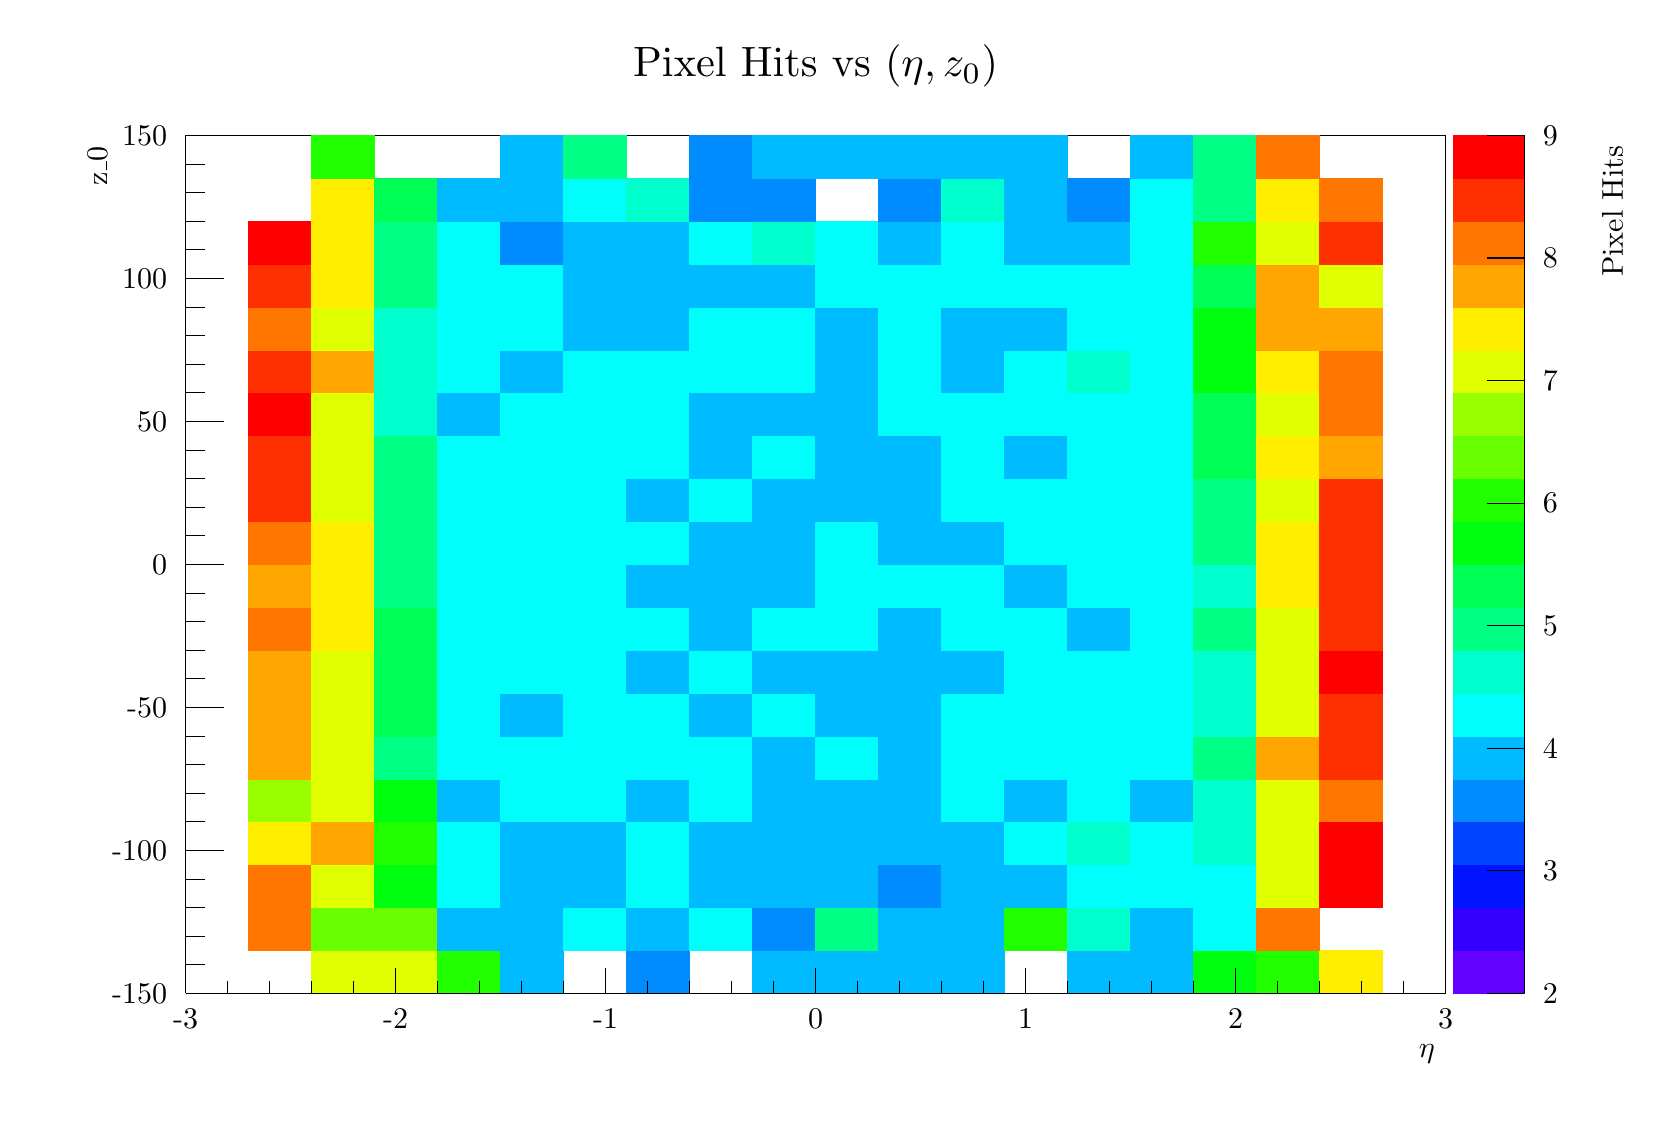
\begin{tikzpicture}
\pgfdeclareplotmark{cross} {
\pgfpathmoveto{\pgfpoint{-0.3\pgfplotmarksize}{\pgfplotmarksize}}
\pgfpathlineto{\pgfpoint{+0.3\pgfplotmarksize}{\pgfplotmarksize}}
\pgfpathlineto{\pgfpoint{+0.3\pgfplotmarksize}{0.3\pgfplotmarksize}}
\pgfpathlineto{\pgfpoint{+1\pgfplotmarksize}{0.3\pgfplotmarksize}}
\pgfpathlineto{\pgfpoint{+1\pgfplotmarksize}{-0.3\pgfplotmarksize}}
\pgfpathlineto{\pgfpoint{+0.3\pgfplotmarksize}{-0.3\pgfplotmarksize}}
\pgfpathlineto{\pgfpoint{+0.3\pgfplotmarksize}{-1.\pgfplotmarksize}}
\pgfpathlineto{\pgfpoint{-0.3\pgfplotmarksize}{-1.\pgfplotmarksize}}
\pgfpathlineto{\pgfpoint{-0.3\pgfplotmarksize}{-0.3\pgfplotmarksize}}
\pgfpathlineto{\pgfpoint{-1.\pgfplotmarksize}{-0.3\pgfplotmarksize}}
\pgfpathlineto{\pgfpoint{-1.\pgfplotmarksize}{0.3\pgfplotmarksize}}
\pgfpathlineto{\pgfpoint{-0.3\pgfplotmarksize}{0.3\pgfplotmarksize}}
\pgfpathclose
\pgfusepathqstroke
}
\pgfdeclareplotmark{cross*} {
\pgfpathmoveto{\pgfpoint{-0.3\pgfplotmarksize}{\pgfplotmarksize}}
\pgfpathlineto{\pgfpoint{+0.3\pgfplotmarksize}{\pgfplotmarksize}}
\pgfpathlineto{\pgfpoint{+0.3\pgfplotmarksize}{0.3\pgfplotmarksize}}
\pgfpathlineto{\pgfpoint{+1\pgfplotmarksize}{0.3\pgfplotmarksize}}
\pgfpathlineto{\pgfpoint{+1\pgfplotmarksize}{-0.3\pgfplotmarksize}}
\pgfpathlineto{\pgfpoint{+0.3\pgfplotmarksize}{-0.3\pgfplotmarksize}}
\pgfpathlineto{\pgfpoint{+0.3\pgfplotmarksize}{-1.\pgfplotmarksize}}
\pgfpathlineto{\pgfpoint{-0.3\pgfplotmarksize}{-1.\pgfplotmarksize}}
\pgfpathlineto{\pgfpoint{-0.3\pgfplotmarksize}{-0.3\pgfplotmarksize}}
\pgfpathlineto{\pgfpoint{-1.\pgfplotmarksize}{-0.3\pgfplotmarksize}}
\pgfpathlineto{\pgfpoint{-1.\pgfplotmarksize}{0.3\pgfplotmarksize}}
\pgfpathlineto{\pgfpoint{-0.3\pgfplotmarksize}{0.3\pgfplotmarksize}}
\pgfpathclose
\pgfusepathqfillstroke
}
\pgfdeclareplotmark{newstar} {
\pgfpathmoveto{\pgfqpoint{0pt}{\pgfplotmarksize}}
\pgfpathlineto{\pgfqpointpolar{44}{0.5\pgfplotmarksize}}
\pgfpathlineto{\pgfqpointpolar{18}{\pgfplotmarksize}}
\pgfpathlineto{\pgfqpointpolar{-20}{0.5\pgfplotmarksize}}
\pgfpathlineto{\pgfqpointpolar{-54}{\pgfplotmarksize}}
\pgfpathlineto{\pgfqpointpolar{-90}{0.5\pgfplotmarksize}}
\pgfpathlineto{\pgfqpointpolar{234}{\pgfplotmarksize}}
\pgfpathlineto{\pgfqpointpolar{198}{0.5\pgfplotmarksize}}
\pgfpathlineto{\pgfqpointpolar{162}{\pgfplotmarksize}}
\pgfpathlineto{\pgfqpointpolar{134}{0.5\pgfplotmarksize}}
\pgfpathclose
\pgfusepathqstroke
}
\pgfdeclareplotmark{newstar*} {
\pgfpathmoveto{\pgfqpoint{0pt}{\pgfplotmarksize}}
\pgfpathlineto{\pgfqpointpolar{44}{0.5\pgfplotmarksize}}
\pgfpathlineto{\pgfqpointpolar{18}{\pgfplotmarksize}}
\pgfpathlineto{\pgfqpointpolar{-20}{0.5\pgfplotmarksize}}
\pgfpathlineto{\pgfqpointpolar{-54}{\pgfplotmarksize}}
\pgfpathlineto{\pgfqpointpolar{-90}{0.5\pgfplotmarksize}}
\pgfpathlineto{\pgfqpointpolar{234}{\pgfplotmarksize}}
\pgfpathlineto{\pgfqpointpolar{198}{0.5\pgfplotmarksize}}
\pgfpathlineto{\pgfqpointpolar{162}{\pgfplotmarksize}}
\pgfpathlineto{\pgfqpointpolar{134}{0.5\pgfplotmarksize}}
\pgfpathclose
\pgfusepathqfillstroke
}
\definecolor{c}{rgb}{1,1,1};
\draw [color=c, fill=c] (0,0) rectangle (20,13.6207);
\draw [color=c, fill=c] (2,1.36207) rectangle (18,12.2586);
\definecolor{c}{rgb}{0,0,0};
\draw [c] (2,1.36207) -- (2,12.2586) -- (18,12.2586) -- (18,1.36207) -- (2,1.36207);
\definecolor{c}{rgb}{1,1,1};
\draw [color=c, fill=c] (2,1.36207) rectangle (18,12.2586);
\definecolor{c}{rgb}{0,0,0};
\draw [c] (2,1.36207) -- (2,12.2586) -- (18,12.2586) -- (18,1.36207) -- (2,1.36207);
\definecolor{c}{rgb}{0.88,1,0};
\draw [color=c, fill=c] (3.6,1.36207) rectangle (4.4,1.9069);
\draw [color=c, fill=c] (4.4,1.36207) rectangle (5.2,1.9069);
\definecolor{c}{rgb}{0.133333,1,0};
\draw [color=c, fill=c] (5.2,1.36207) rectangle (6,1.9069);
\definecolor{c}{rgb}{0,0.733333,1};
\draw [color=c, fill=c] (6,1.36207) rectangle (6.8,1.9069);
\definecolor{c}{rgb}{0,0.546666,1};
\draw [color=c, fill=c] (7.6,1.36207) rectangle (8.4,1.9069);
\definecolor{c}{rgb}{0,0.733333,1};
\draw [color=c, fill=c] (9.2,1.36207) rectangle (10,1.9069);
\draw [color=c, fill=c] (10,1.36207) rectangle (10.8,1.9069);
\draw [color=c, fill=c] (10.8,1.36207) rectangle (11.6,1.9069);
\draw [color=c, fill=c] (11.6,1.36207) rectangle (12.4,1.9069);
\draw [color=c, fill=c] (13.2,1.36207) rectangle (14,1.9069);
\draw [color=c, fill=c] (14,1.36207) rectangle (14.8,1.9069);
\definecolor{c}{rgb}{0,1,0.0533333};
\draw [color=c, fill=c] (14.8,1.36207) rectangle (15.6,1.9069);
\definecolor{c}{rgb}{0.133333,1,0};
\draw [color=c, fill=c] (15.6,1.36207) rectangle (16.4,1.9069);
\definecolor{c}{rgb}{1,0.933333,0};
\draw [color=c, fill=c] (16.4,1.36207) rectangle (17.2,1.9069);
\definecolor{c}{rgb}{1,0.466667,0};
\draw [color=c, fill=c] (2.8,1.9069) rectangle (3.6,2.45172);
\definecolor{c}{rgb}{0.413333,1,0};
\draw [color=c, fill=c] (3.6,1.9069) rectangle (4.4,2.45172);
\draw [color=c, fill=c] (4.4,1.9069) rectangle (5.2,2.45172);
\definecolor{c}{rgb}{0,0.733333,1};
\draw [color=c, fill=c] (5.2,1.9069) rectangle (6,2.45172);
\draw [color=c, fill=c] (6,1.9069) rectangle (6.8,2.45172);
\definecolor{c}{rgb}{0,1,0.986667};
\draw [color=c, fill=c] (6.8,1.9069) rectangle (7.6,2.45172);
\definecolor{c}{rgb}{0,0.733333,1};
\draw [color=c, fill=c] (7.6,1.9069) rectangle (8.4,2.45172);
\definecolor{c}{rgb}{0,1,0.986667};
\draw [color=c, fill=c] (8.4,1.9069) rectangle (9.2,2.45172);
\definecolor{c}{rgb}{0,0.546666,1};
\draw [color=c, fill=c] (9.2,1.9069) rectangle (10,2.45172);
\definecolor{c}{rgb}{0,1,0.52};
\draw [color=c, fill=c] (10,1.9069) rectangle (10.8,2.45172);
\definecolor{c}{rgb}{0,0.733333,1};
\draw [color=c, fill=c] (10.8,1.9069) rectangle (11.6,2.45172);
\draw [color=c, fill=c] (11.6,1.9069) rectangle (12.4,2.45172);
\definecolor{c}{rgb}{0.133333,1,0};
\draw [color=c, fill=c] (12.4,1.9069) rectangle (13.2,2.45172);
\definecolor{c}{rgb}{0,1,0.8};
\draw [color=c, fill=c] (13.2,1.9069) rectangle (14,2.45172);
\definecolor{c}{rgb}{0,0.733333,1};
\draw [color=c, fill=c] (14,1.9069) rectangle (14.8,2.45172);
\definecolor{c}{rgb}{0,1,0.986667};
\draw [color=c, fill=c] (14.8,1.9069) rectangle (15.6,2.45172);
\definecolor{c}{rgb}{1,0.466667,0};
\draw [color=c, fill=c] (15.6,1.9069) rectangle (16.4,2.45172);
\draw [color=c, fill=c] (2.8,2.45172) rectangle (3.6,2.99655);
\definecolor{c}{rgb}{0.88,1,0};
\draw [color=c, fill=c] (3.6,2.45172) rectangle (4.4,2.99655);
\definecolor{c}{rgb}{0,1,0.0533333};
\draw [color=c, fill=c] (4.4,2.45172) rectangle (5.2,2.99655);
\definecolor{c}{rgb}{0,1,0.986667};
\draw [color=c, fill=c] (5.2,2.45172) rectangle (6,2.99655);
\definecolor{c}{rgb}{0,0.733333,1};
\draw [color=c, fill=c] (6,2.45172) rectangle (6.8,2.99655);
\draw [color=c, fill=c] (6.8,2.45172) rectangle (7.6,2.99655);
\definecolor{c}{rgb}{0,1,0.986667};
\draw [color=c, fill=c] (7.6,2.45172) rectangle (8.4,2.99655);
\definecolor{c}{rgb}{0,0.733333,1};
\draw [color=c, fill=c] (8.4,2.45172) rectangle (9.2,2.99655);
\draw [color=c, fill=c] (9.2,2.45172) rectangle (10,2.99655);
\draw [color=c, fill=c] (10,2.45172) rectangle (10.8,2.99655);
\definecolor{c}{rgb}{0,0.546666,1};
\draw [color=c, fill=c] (10.8,2.45172) rectangle (11.6,2.99655);
\definecolor{c}{rgb}{0,0.733333,1};
\draw [color=c, fill=c] (11.6,2.45172) rectangle (12.4,2.99655);
\draw [color=c, fill=c] (12.4,2.45172) rectangle (13.2,2.99655);
\definecolor{c}{rgb}{0,1,0.986667};
\draw [color=c, fill=c] (13.2,2.45172) rectangle (14,2.99655);
\draw [color=c, fill=c] (14,2.45172) rectangle (14.8,2.99655);
\draw [color=c, fill=c] (14.8,2.45172) rectangle (15.6,2.99655);
\definecolor{c}{rgb}{0.88,1,0};
\draw [color=c, fill=c] (15.6,2.45172) rectangle (16.4,2.99655);
\definecolor{c}{rgb}{1,0,0};
\draw [color=c, fill=c] (16.4,2.45172) rectangle (17.2,2.99655);
\definecolor{c}{rgb}{1,0.933333,0};
\draw [color=c, fill=c] (2.8,2.99655) rectangle (3.6,3.54138);
\definecolor{c}{rgb}{1,0.653333,0};
\draw [color=c, fill=c] (3.6,2.99655) rectangle (4.4,3.54138);
\definecolor{c}{rgb}{0.133333,1,0};
\draw [color=c, fill=c] (4.4,2.99655) rectangle (5.2,3.54138);
\definecolor{c}{rgb}{0,1,0.986667};
\draw [color=c, fill=c] (5.2,2.99655) rectangle (6,3.54138);
\definecolor{c}{rgb}{0,0.733333,1};
\draw [color=c, fill=c] (6,2.99655) rectangle (6.8,3.54138);
\draw [color=c, fill=c] (6.8,2.99655) rectangle (7.6,3.54138);
\definecolor{c}{rgb}{0,1,0.986667};
\draw [color=c, fill=c] (7.6,2.99655) rectangle (8.4,3.54138);
\definecolor{c}{rgb}{0,0.733333,1};
\draw [color=c, fill=c] (8.4,2.99655) rectangle (9.2,3.54138);
\draw [color=c, fill=c] (9.2,2.99655) rectangle (10,3.54138);
\draw [color=c, fill=c] (10,2.99655) rectangle (10.8,3.54138);
\draw [color=c, fill=c] (10.8,2.99655) rectangle (11.6,3.54138);
\draw [color=c, fill=c] (11.6,2.99655) rectangle (12.4,3.54138);
\definecolor{c}{rgb}{0,1,0.986667};
\draw [color=c, fill=c] (12.4,2.99655) rectangle (13.2,3.54138);
\definecolor{c}{rgb}{0,1,0.8};
\draw [color=c, fill=c] (13.2,2.99655) rectangle (14,3.54138);
\definecolor{c}{rgb}{0,1,0.986667};
\draw [color=c, fill=c] (14,2.99655) rectangle (14.8,3.54138);
\definecolor{c}{rgb}{0,1,0.8};
\draw [color=c, fill=c] (14.8,2.99655) rectangle (15.6,3.54138);
\definecolor{c}{rgb}{0.88,1,0};
\draw [color=c, fill=c] (15.6,2.99655) rectangle (16.4,3.54138);
\definecolor{c}{rgb}{1,0,0};
\draw [color=c, fill=c] (16.4,2.99655) rectangle (17.2,3.54138);
\definecolor{c}{rgb}{0.6,1,0};
\draw [color=c, fill=c] (2.8,3.54138) rectangle (3.6,4.08621);
\definecolor{c}{rgb}{0.88,1,0};
\draw [color=c, fill=c] (3.6,3.54138) rectangle (4.4,4.08621);
\definecolor{c}{rgb}{0,1,0.0533333};
\draw [color=c, fill=c] (4.4,3.54138) rectangle (5.2,4.08621);
\definecolor{c}{rgb}{0,0.733333,1};
\draw [color=c, fill=c] (5.2,3.54138) rectangle (6,4.08621);
\definecolor{c}{rgb}{0,1,0.986667};
\draw [color=c, fill=c] (6,3.54138) rectangle (6.8,4.08621);
\draw [color=c, fill=c] (6.8,3.54138) rectangle (7.6,4.08621);
\definecolor{c}{rgb}{0,0.733333,1};
\draw [color=c, fill=c] (7.6,3.54138) rectangle (8.4,4.08621);
\definecolor{c}{rgb}{0,1,0.986667};
\draw [color=c, fill=c] (8.4,3.54138) rectangle (9.2,4.08621);
\definecolor{c}{rgb}{0,0.733333,1};
\draw [color=c, fill=c] (9.2,3.54138) rectangle (10,4.08621);
\draw [color=c, fill=c] (10,3.54138) rectangle (10.8,4.08621);
\draw [color=c, fill=c] (10.8,3.54138) rectangle (11.6,4.08621);
\definecolor{c}{rgb}{0,1,0.986667};
\draw [color=c, fill=c] (11.6,3.54138) rectangle (12.4,4.08621);
\definecolor{c}{rgb}{0,0.733333,1};
\draw [color=c, fill=c] (12.4,3.54138) rectangle (13.2,4.08621);
\definecolor{c}{rgb}{0,1,0.986667};
\draw [color=c, fill=c] (13.2,3.54138) rectangle (14,4.08621);
\definecolor{c}{rgb}{0,0.733333,1};
\draw [color=c, fill=c] (14,3.54138) rectangle (14.8,4.08621);
\definecolor{c}{rgb}{0,1,0.8};
\draw [color=c, fill=c] (14.8,3.54138) rectangle (15.6,4.08621);
\definecolor{c}{rgb}{0.88,1,0};
\draw [color=c, fill=c] (15.6,3.54138) rectangle (16.4,4.08621);
\definecolor{c}{rgb}{1,0.466667,0};
\draw [color=c, fill=c] (16.4,3.54138) rectangle (17.2,4.08621);
\definecolor{c}{rgb}{1,0.653333,0};
\draw [color=c, fill=c] (2.8,4.08621) rectangle (3.6,4.63103);
\definecolor{c}{rgb}{0.88,1,0};
\draw [color=c, fill=c] (3.6,4.08621) rectangle (4.4,4.63103);
\definecolor{c}{rgb}{0,1,0.52};
\draw [color=c, fill=c] (4.4,4.08621) rectangle (5.2,4.63103);
\definecolor{c}{rgb}{0,1,0.986667};
\draw [color=c, fill=c] (5.2,4.08621) rectangle (6,4.63103);
\draw [color=c, fill=c] (6,4.08621) rectangle (6.8,4.63103);
\draw [color=c, fill=c] (6.8,4.08621) rectangle (7.6,4.63103);
\draw [color=c, fill=c] (7.6,4.08621) rectangle (8.4,4.63103);
\draw [color=c, fill=c] (8.4,4.08621) rectangle (9.2,4.63103);
\definecolor{c}{rgb}{0,0.733333,1};
\draw [color=c, fill=c] (9.2,4.08621) rectangle (10,4.63103);
\definecolor{c}{rgb}{0,1,0.986667};
\draw [color=c, fill=c] (10,4.08621) rectangle (10.8,4.63103);
\definecolor{c}{rgb}{0,0.733333,1};
\draw [color=c, fill=c] (10.8,4.08621) rectangle (11.6,4.63103);
\definecolor{c}{rgb}{0,1,0.986667};
\draw [color=c, fill=c] (11.6,4.08621) rectangle (12.4,4.63103);
\draw [color=c, fill=c] (12.4,4.08621) rectangle (13.2,4.63103);
\draw [color=c, fill=c] (13.2,4.08621) rectangle (14,4.63103);
\draw [color=c, fill=c] (14,4.08621) rectangle (14.8,4.63103);
\definecolor{c}{rgb}{0,1,0.52};
\draw [color=c, fill=c] (14.8,4.08621) rectangle (15.6,4.63103);
\definecolor{c}{rgb}{1,0.653333,0};
\draw [color=c, fill=c] (15.6,4.08621) rectangle (16.4,4.63103);
\definecolor{c}{rgb}{1,0.186667,0};
\draw [color=c, fill=c] (16.4,4.08621) rectangle (17.2,4.63103);
\definecolor{c}{rgb}{1,0.653333,0};
\draw [color=c, fill=c] (2.8,4.63103) rectangle (3.6,5.17586);
\definecolor{c}{rgb}{0.88,1,0};
\draw [color=c, fill=c] (3.6,4.63103) rectangle (4.4,5.17586);
\definecolor{c}{rgb}{0,1,0.333333};
\draw [color=c, fill=c] (4.4,4.63103) rectangle (5.2,5.17586);
\definecolor{c}{rgb}{0,1,0.986667};
\draw [color=c, fill=c] (5.2,4.63103) rectangle (6,5.17586);
\definecolor{c}{rgb}{0,0.733333,1};
\draw [color=c, fill=c] (6,4.63103) rectangle (6.8,5.17586);
\definecolor{c}{rgb}{0,1,0.986667};
\draw [color=c, fill=c] (6.8,4.63103) rectangle (7.6,5.17586);
\draw [color=c, fill=c] (7.6,4.63103) rectangle (8.4,5.17586);
\definecolor{c}{rgb}{0,0.733333,1};
\draw [color=c, fill=c] (8.4,4.63103) rectangle (9.2,5.17586);
\definecolor{c}{rgb}{0,1,0.986667};
\draw [color=c, fill=c] (9.2,4.63103) rectangle (10,5.17586);
\definecolor{c}{rgb}{0,0.733333,1};
\draw [color=c, fill=c] (10,4.63103) rectangle (10.8,5.17586);
\draw [color=c, fill=c] (10.8,4.63103) rectangle (11.6,5.17586);
\definecolor{c}{rgb}{0,1,0.986667};
\draw [color=c, fill=c] (11.6,4.63103) rectangle (12.4,5.17586);
\draw [color=c, fill=c] (12.4,4.63103) rectangle (13.2,5.17586);
\draw [color=c, fill=c] (13.2,4.63103) rectangle (14,5.17586);
\draw [color=c, fill=c] (14,4.63103) rectangle (14.8,5.17586);
\definecolor{c}{rgb}{0,1,0.8};
\draw [color=c, fill=c] (14.8,4.63103) rectangle (15.6,5.17586);
\definecolor{c}{rgb}{0.88,1,0};
\draw [color=c, fill=c] (15.6,4.63103) rectangle (16.4,5.17586);
\definecolor{c}{rgb}{1,0.186667,0};
\draw [color=c, fill=c] (16.4,4.63103) rectangle (17.2,5.17586);
\definecolor{c}{rgb}{1,0.653333,0};
\draw [color=c, fill=c] (2.8,5.17586) rectangle (3.6,5.72069);
\definecolor{c}{rgb}{0.88,1,0};
\draw [color=c, fill=c] (3.6,5.17586) rectangle (4.4,5.72069);
\definecolor{c}{rgb}{0,1,0.333333};
\draw [color=c, fill=c] (4.4,5.17586) rectangle (5.2,5.72069);
\definecolor{c}{rgb}{0,1,0.986667};
\draw [color=c, fill=c] (5.2,5.17586) rectangle (6,5.72069);
\draw [color=c, fill=c] (6,5.17586) rectangle (6.8,5.72069);
\draw [color=c, fill=c] (6.8,5.17586) rectangle (7.6,5.72069);
\definecolor{c}{rgb}{0,0.733333,1};
\draw [color=c, fill=c] (7.6,5.17586) rectangle (8.4,5.72069);
\definecolor{c}{rgb}{0,1,0.986667};
\draw [color=c, fill=c] (8.4,5.17586) rectangle (9.2,5.72069);
\definecolor{c}{rgb}{0,0.733333,1};
\draw [color=c, fill=c] (9.2,5.17586) rectangle (10,5.72069);
\draw [color=c, fill=c] (10,5.17586) rectangle (10.8,5.72069);
\draw [color=c, fill=c] (10.8,5.17586) rectangle (11.6,5.72069);
\draw [color=c, fill=c] (11.6,5.17586) rectangle (12.4,5.72069);
\definecolor{c}{rgb}{0,1,0.986667};
\draw [color=c, fill=c] (12.4,5.17586) rectangle (13.2,5.72069);
\draw [color=c, fill=c] (13.2,5.17586) rectangle (14,5.72069);
\draw [color=c, fill=c] (14,5.17586) rectangle (14.8,5.72069);
\definecolor{c}{rgb}{0,1,0.8};
\draw [color=c, fill=c] (14.8,5.17586) rectangle (15.6,5.72069);
\definecolor{c}{rgb}{0.88,1,0};
\draw [color=c, fill=c] (15.6,5.17586) rectangle (16.4,5.72069);
\definecolor{c}{rgb}{1,0,0};
\draw [color=c, fill=c] (16.4,5.17586) rectangle (17.2,5.72069);
\definecolor{c}{rgb}{1,0.466667,0};
\draw [color=c, fill=c] (2.8,5.72069) rectangle (3.6,6.26552);
\definecolor{c}{rgb}{1,0.933333,0};
\draw [color=c, fill=c] (3.6,5.72069) rectangle (4.4,6.26552);
\definecolor{c}{rgb}{0,1,0.333333};
\draw [color=c, fill=c] (4.4,5.72069) rectangle (5.2,6.26552);
\definecolor{c}{rgb}{0,1,0.986667};
\draw [color=c, fill=c] (5.2,5.72069) rectangle (6,6.26552);
\draw [color=c, fill=c] (6,5.72069) rectangle (6.8,6.26552);
\draw [color=c, fill=c] (6.8,5.72069) rectangle (7.6,6.26552);
\draw [color=c, fill=c] (7.6,5.72069) rectangle (8.4,6.26552);
\definecolor{c}{rgb}{0,0.733333,1};
\draw [color=c, fill=c] (8.4,5.72069) rectangle (9.2,6.26552);
\definecolor{c}{rgb}{0,1,0.986667};
\draw [color=c, fill=c] (9.2,5.72069) rectangle (10,6.26552);
\draw [color=c, fill=c] (10,5.72069) rectangle (10.8,6.26552);
\definecolor{c}{rgb}{0,0.733333,1};
\draw [color=c, fill=c] (10.8,5.72069) rectangle (11.6,6.26552);
\definecolor{c}{rgb}{0,1,0.986667};
\draw [color=c, fill=c] (11.6,5.72069) rectangle (12.4,6.26552);
\draw [color=c, fill=c] (12.4,5.72069) rectangle (13.2,6.26552);
\definecolor{c}{rgb}{0,0.733333,1};
\draw [color=c, fill=c] (13.2,5.72069) rectangle (14,6.26552);
\definecolor{c}{rgb}{0,1,0.986667};
\draw [color=c, fill=c] (14,5.72069) rectangle (14.8,6.26552);
\definecolor{c}{rgb}{0,1,0.52};
\draw [color=c, fill=c] (14.8,5.72069) rectangle (15.6,6.26552);
\definecolor{c}{rgb}{0.88,1,0};
\draw [color=c, fill=c] (15.6,5.72069) rectangle (16.4,6.26552);
\definecolor{c}{rgb}{1,0.186667,0};
\draw [color=c, fill=c] (16.4,5.72069) rectangle (17.2,6.26552);
\definecolor{c}{rgb}{1,0.653333,0};
\draw [color=c, fill=c] (2.8,6.26552) rectangle (3.6,6.81034);
\definecolor{c}{rgb}{1,0.933333,0};
\draw [color=c, fill=c] (3.6,6.26552) rectangle (4.4,6.81034);
\definecolor{c}{rgb}{0,1,0.52};
\draw [color=c, fill=c] (4.4,6.26552) rectangle (5.2,6.81034);
\definecolor{c}{rgb}{0,1,0.986667};
\draw [color=c, fill=c] (5.2,6.26552) rectangle (6,6.81034);
\draw [color=c, fill=c] (6,6.26552) rectangle (6.8,6.81034);
\draw [color=c, fill=c] (6.8,6.26552) rectangle (7.6,6.81034);
\definecolor{c}{rgb}{0,0.733333,1};
\draw [color=c, fill=c] (7.6,6.26552) rectangle (8.4,6.81034);
\draw [color=c, fill=c] (8.4,6.26552) rectangle (9.2,6.81034);
\draw [color=c, fill=c] (9.2,6.26552) rectangle (10,6.81034);
\definecolor{c}{rgb}{0,1,0.986667};
\draw [color=c, fill=c] (10,6.26552) rectangle (10.8,6.81034);
\draw [color=c, fill=c] (10.8,6.26552) rectangle (11.6,6.81034);
\draw [color=c, fill=c] (11.6,6.26552) rectangle (12.4,6.81034);
\definecolor{c}{rgb}{0,0.733333,1};
\draw [color=c, fill=c] (12.4,6.26552) rectangle (13.2,6.81034);
\definecolor{c}{rgb}{0,1,0.986667};
\draw [color=c, fill=c] (13.2,6.26552) rectangle (14,6.81034);
\draw [color=c, fill=c] (14,6.26552) rectangle (14.8,6.81034);
\definecolor{c}{rgb}{0,1,0.8};
\draw [color=c, fill=c] (14.8,6.26552) rectangle (15.6,6.81034);
\definecolor{c}{rgb}{1,0.933333,0};
\draw [color=c, fill=c] (15.6,6.26552) rectangle (16.4,6.81034);
\definecolor{c}{rgb}{1,0.186667,0};
\draw [color=c, fill=c] (16.4,6.26552) rectangle (17.2,6.81034);
\definecolor{c}{rgb}{1,0.466667,0};
\draw [color=c, fill=c] (2.8,6.81034) rectangle (3.6,7.35517);
\definecolor{c}{rgb}{1,0.933333,0};
\draw [color=c, fill=c] (3.6,6.81034) rectangle (4.4,7.35517);
\definecolor{c}{rgb}{0,1,0.52};
\draw [color=c, fill=c] (4.4,6.81034) rectangle (5.2,7.35517);
\definecolor{c}{rgb}{0,1,0.986667};
\draw [color=c, fill=c] (5.2,6.81034) rectangle (6,7.35517);
\draw [color=c, fill=c] (6,6.81034) rectangle (6.8,7.35517);
\draw [color=c, fill=c] (6.8,6.81034) rectangle (7.6,7.35517);
\draw [color=c, fill=c] (7.6,6.81034) rectangle (8.4,7.35517);
\definecolor{c}{rgb}{0,0.733333,1};
\draw [color=c, fill=c] (8.4,6.81034) rectangle (9.2,7.35517);
\draw [color=c, fill=c] (9.2,6.81034) rectangle (10,7.35517);
\definecolor{c}{rgb}{0,1,0.986667};
\draw [color=c, fill=c] (10,6.81034) rectangle (10.8,7.35517);
\definecolor{c}{rgb}{0,0.733333,1};
\draw [color=c, fill=c] (10.8,6.81034) rectangle (11.6,7.35517);
\draw [color=c, fill=c] (11.6,6.81034) rectangle (12.4,7.35517);
\definecolor{c}{rgb}{0,1,0.986667};
\draw [color=c, fill=c] (12.4,6.81034) rectangle (13.2,7.35517);
\draw [color=c, fill=c] (13.2,6.81034) rectangle (14,7.35517);
\draw [color=c, fill=c] (14,6.81034) rectangle (14.8,7.35517);
\definecolor{c}{rgb}{0,1,0.52};
\draw [color=c, fill=c] (14.8,6.81034) rectangle (15.6,7.35517);
\definecolor{c}{rgb}{1,0.933333,0};
\draw [color=c, fill=c] (15.6,6.81034) rectangle (16.4,7.35517);
\definecolor{c}{rgb}{1,0.186667,0};
\draw [color=c, fill=c] (16.4,6.81034) rectangle (17.2,7.35517);
\draw [color=c, fill=c] (2.8,7.35517) rectangle (3.6,7.9);
\definecolor{c}{rgb}{0.88,1,0};
\draw [color=c, fill=c] (3.6,7.35517) rectangle (4.4,7.9);
\definecolor{c}{rgb}{0,1,0.52};
\draw [color=c, fill=c] (4.4,7.35517) rectangle (5.2,7.9);
\definecolor{c}{rgb}{0,1,0.986667};
\draw [color=c, fill=c] (5.2,7.35517) rectangle (6,7.9);
\draw [color=c, fill=c] (6,7.35517) rectangle (6.8,7.9);
\draw [color=c, fill=c] (6.8,7.35517) rectangle (7.6,7.9);
\definecolor{c}{rgb}{0,0.733333,1};
\draw [color=c, fill=c] (7.6,7.35517) rectangle (8.4,7.9);
\definecolor{c}{rgb}{0,1,0.986667};
\draw [color=c, fill=c] (8.4,7.35517) rectangle (9.2,7.9);
\definecolor{c}{rgb}{0,0.733333,1};
\draw [color=c, fill=c] (9.2,7.35517) rectangle (10,7.9);
\draw [color=c, fill=c] (10,7.35517) rectangle (10.8,7.9);
\draw [color=c, fill=c] (10.8,7.35517) rectangle (11.6,7.9);
\definecolor{c}{rgb}{0,1,0.986667};
\draw [color=c, fill=c] (11.6,7.35517) rectangle (12.4,7.9);
\draw [color=c, fill=c] (12.4,7.35517) rectangle (13.2,7.9);
\draw [color=c, fill=c] (13.2,7.35517) rectangle (14,7.9);
\draw [color=c, fill=c] (14,7.35517) rectangle (14.8,7.9);
\definecolor{c}{rgb}{0,1,0.52};
\draw [color=c, fill=c] (14.8,7.35517) rectangle (15.6,7.9);
\definecolor{c}{rgb}{0.88,1,0};
\draw [color=c, fill=c] (15.6,7.35517) rectangle (16.4,7.9);
\definecolor{c}{rgb}{1,0.186667,0};
\draw [color=c, fill=c] (16.4,7.35517) rectangle (17.2,7.9);
\draw [color=c, fill=c] (2.8,7.9) rectangle (3.6,8.44483);
\definecolor{c}{rgb}{0.88,1,0};
\draw [color=c, fill=c] (3.6,7.9) rectangle (4.4,8.44483);
\definecolor{c}{rgb}{0,1,0.52};
\draw [color=c, fill=c] (4.4,7.9) rectangle (5.2,8.44483);
\definecolor{c}{rgb}{0,1,0.986667};
\draw [color=c, fill=c] (5.2,7.9) rectangle (6,8.44483);
\draw [color=c, fill=c] (6,7.9) rectangle (6.8,8.44483);
\draw [color=c, fill=c] (6.8,7.9) rectangle (7.6,8.44483);
\draw [color=c, fill=c] (7.6,7.9) rectangle (8.4,8.44483);
\definecolor{c}{rgb}{0,0.733333,1};
\draw [color=c, fill=c] (8.4,7.9) rectangle (9.2,8.44483);
\definecolor{c}{rgb}{0,1,0.986667};
\draw [color=c, fill=c] (9.2,7.9) rectangle (10,8.44483);
\definecolor{c}{rgb}{0,0.733333,1};
\draw [color=c, fill=c] (10,7.9) rectangle (10.8,8.44483);
\draw [color=c, fill=c] (10.8,7.9) rectangle (11.6,8.44483);
\definecolor{c}{rgb}{0,1,0.986667};
\draw [color=c, fill=c] (11.6,7.9) rectangle (12.4,8.44483);
\definecolor{c}{rgb}{0,0.733333,1};
\draw [color=c, fill=c] (12.4,7.9) rectangle (13.2,8.44483);
\definecolor{c}{rgb}{0,1,0.986667};
\draw [color=c, fill=c] (13.2,7.9) rectangle (14,8.44483);
\draw [color=c, fill=c] (14,7.9) rectangle (14.8,8.44483);
\definecolor{c}{rgb}{0,1,0.333333};
\draw [color=c, fill=c] (14.8,7.9) rectangle (15.6,8.44483);
\definecolor{c}{rgb}{1,0.933333,0};
\draw [color=c, fill=c] (15.6,7.9) rectangle (16.4,8.44483);
\definecolor{c}{rgb}{1,0.653333,0};
\draw [color=c, fill=c] (16.4,7.9) rectangle (17.2,8.44483);
\definecolor{c}{rgb}{1,0,0};
\draw [color=c, fill=c] (2.8,8.44483) rectangle (3.6,8.98965);
\definecolor{c}{rgb}{0.88,1,0};
\draw [color=c, fill=c] (3.6,8.44483) rectangle (4.4,8.98965);
\definecolor{c}{rgb}{0,1,0.8};
\draw [color=c, fill=c] (4.4,8.44483) rectangle (5.2,8.98965);
\definecolor{c}{rgb}{0,0.733333,1};
\draw [color=c, fill=c] (5.2,8.44483) rectangle (6,8.98965);
\definecolor{c}{rgb}{0,1,0.986667};
\draw [color=c, fill=c] (6,8.44483) rectangle (6.8,8.98965);
\draw [color=c, fill=c] (6.8,8.44483) rectangle (7.6,8.98965);
\draw [color=c, fill=c] (7.6,8.44483) rectangle (8.4,8.98965);
\definecolor{c}{rgb}{0,0.733333,1};
\draw [color=c, fill=c] (8.4,8.44483) rectangle (9.2,8.98965);
\draw [color=c, fill=c] (9.2,8.44483) rectangle (10,8.98965);
\draw [color=c, fill=c] (10,8.44483) rectangle (10.8,8.98965);
\definecolor{c}{rgb}{0,1,0.986667};
\draw [color=c, fill=c] (10.8,8.44483) rectangle (11.6,8.98965);
\draw [color=c, fill=c] (11.6,8.44483) rectangle (12.4,8.98965);
\draw [color=c, fill=c] (12.4,8.44483) rectangle (13.2,8.98965);
\draw [color=c, fill=c] (13.2,8.44483) rectangle (14,8.98965);
\draw [color=c, fill=c] (14,8.44483) rectangle (14.8,8.98965);
\definecolor{c}{rgb}{0,1,0.333333};
\draw [color=c, fill=c] (14.8,8.44483) rectangle (15.6,8.98965);
\definecolor{c}{rgb}{0.88,1,0};
\draw [color=c, fill=c] (15.6,8.44483) rectangle (16.4,8.98965);
\definecolor{c}{rgb}{1,0.466667,0};
\draw [color=c, fill=c] (16.4,8.44483) rectangle (17.2,8.98965);
\definecolor{c}{rgb}{1,0.186667,0};
\draw [color=c, fill=c] (2.8,8.98965) rectangle (3.6,9.53448);
\definecolor{c}{rgb}{1,0.653333,0};
\draw [color=c, fill=c] (3.6,8.98965) rectangle (4.4,9.53448);
\definecolor{c}{rgb}{0,1,0.8};
\draw [color=c, fill=c] (4.4,8.98965) rectangle (5.2,9.53448);
\definecolor{c}{rgb}{0,1,0.986667};
\draw [color=c, fill=c] (5.2,8.98965) rectangle (6,9.53448);
\definecolor{c}{rgb}{0,0.733333,1};
\draw [color=c, fill=c] (6,8.98965) rectangle (6.8,9.53448);
\definecolor{c}{rgb}{0,1,0.986667};
\draw [color=c, fill=c] (6.8,8.98965) rectangle (7.6,9.53448);
\draw [color=c, fill=c] (7.6,8.98965) rectangle (8.4,9.53448);
\draw [color=c, fill=c] (8.4,8.98965) rectangle (9.2,9.53448);
\draw [color=c, fill=c] (9.2,8.98965) rectangle (10,9.53448);
\definecolor{c}{rgb}{0,0.733333,1};
\draw [color=c, fill=c] (10,8.98965) rectangle (10.8,9.53448);
\definecolor{c}{rgb}{0,1,0.986667};
\draw [color=c, fill=c] (10.8,8.98965) rectangle (11.6,9.53448);
\definecolor{c}{rgb}{0,0.733333,1};
\draw [color=c, fill=c] (11.6,8.98965) rectangle (12.4,9.53448);
\definecolor{c}{rgb}{0,1,0.986667};
\draw [color=c, fill=c] (12.4,8.98965) rectangle (13.2,9.53448);
\definecolor{c}{rgb}{0,1,0.8};
\draw [color=c, fill=c] (13.2,8.98965) rectangle (14,9.53448);
\definecolor{c}{rgb}{0,1,0.986667};
\draw [color=c, fill=c] (14,8.98965) rectangle (14.8,9.53448);
\definecolor{c}{rgb}{0,1,0.0533333};
\draw [color=c, fill=c] (14.8,8.98965) rectangle (15.6,9.53448);
\definecolor{c}{rgb}{1,0.933333,0};
\draw [color=c, fill=c] (15.6,8.98965) rectangle (16.4,9.53448);
\definecolor{c}{rgb}{1,0.466667,0};
\draw [color=c, fill=c] (16.4,8.98965) rectangle (17.2,9.53448);
\draw [color=c, fill=c] (2.8,9.53448) rectangle (3.6,10.0793);
\definecolor{c}{rgb}{0.88,1,0};
\draw [color=c, fill=c] (3.6,9.53448) rectangle (4.4,10.0793);
\definecolor{c}{rgb}{0,1,0.8};
\draw [color=c, fill=c] (4.4,9.53448) rectangle (5.2,10.0793);
\definecolor{c}{rgb}{0,1,0.986667};
\draw [color=c, fill=c] (5.2,9.53448) rectangle (6,10.0793);
\draw [color=c, fill=c] (6,9.53448) rectangle (6.8,10.0793);
\definecolor{c}{rgb}{0,0.733333,1};
\draw [color=c, fill=c] (6.8,9.53448) rectangle (7.6,10.0793);
\draw [color=c, fill=c] (7.6,9.53448) rectangle (8.4,10.0793);
\definecolor{c}{rgb}{0,1,0.986667};
\draw [color=c, fill=c] (8.4,9.53448) rectangle (9.2,10.0793);
\draw [color=c, fill=c] (9.2,9.53448) rectangle (10,10.0793);
\definecolor{c}{rgb}{0,0.733333,1};
\draw [color=c, fill=c] (10,9.53448) rectangle (10.8,10.0793);
\definecolor{c}{rgb}{0,1,0.986667};
\draw [color=c, fill=c] (10.8,9.53448) rectangle (11.6,10.0793);
\definecolor{c}{rgb}{0,0.733333,1};
\draw [color=c, fill=c] (11.6,9.53448) rectangle (12.4,10.0793);
\draw [color=c, fill=c] (12.4,9.53448) rectangle (13.2,10.0793);
\definecolor{c}{rgb}{0,1,0.986667};
\draw [color=c, fill=c] (13.2,9.53448) rectangle (14,10.0793);
\draw [color=c, fill=c] (14,9.53448) rectangle (14.8,10.0793);
\definecolor{c}{rgb}{0,1,0.0533333};
\draw [color=c, fill=c] (14.8,9.53448) rectangle (15.6,10.0793);
\definecolor{c}{rgb}{1,0.653333,0};
\draw [color=c, fill=c] (15.6,9.53448) rectangle (16.4,10.0793);
\draw [color=c, fill=c] (16.4,9.53448) rectangle (17.2,10.0793);
\definecolor{c}{rgb}{1,0.186667,0};
\draw [color=c, fill=c] (2.8,10.0793) rectangle (3.6,10.6241);
\definecolor{c}{rgb}{1,0.933333,0};
\draw [color=c, fill=c] (3.6,10.0793) rectangle (4.4,10.6241);
\definecolor{c}{rgb}{0,1,0.52};
\draw [color=c, fill=c] (4.4,10.0793) rectangle (5.2,10.6241);
\definecolor{c}{rgb}{0,1,0.986667};
\draw [color=c, fill=c] (5.2,10.0793) rectangle (6,10.6241);
\draw [color=c, fill=c] (6,10.0793) rectangle (6.8,10.6241);
\definecolor{c}{rgb}{0,0.733333,1};
\draw [color=c, fill=c] (6.8,10.0793) rectangle (7.6,10.6241);
\draw [color=c, fill=c] (7.6,10.0793) rectangle (8.4,10.6241);
\draw [color=c, fill=c] (8.4,10.0793) rectangle (9.2,10.6241);
\draw [color=c, fill=c] (9.2,10.0793) rectangle (10,10.6241);
\definecolor{c}{rgb}{0,1,0.986667};
\draw [color=c, fill=c] (10,10.0793) rectangle (10.8,10.6241);
\draw [color=c, fill=c] (10.8,10.0793) rectangle (11.6,10.6241);
\draw [color=c, fill=c] (11.6,10.0793) rectangle (12.4,10.6241);
\draw [color=c, fill=c] (12.4,10.0793) rectangle (13.2,10.6241);
\draw [color=c, fill=c] (13.2,10.0793) rectangle (14,10.6241);
\draw [color=c, fill=c] (14,10.0793) rectangle (14.8,10.6241);
\definecolor{c}{rgb}{0,1,0.333333};
\draw [color=c, fill=c] (14.8,10.0793) rectangle (15.6,10.6241);
\definecolor{c}{rgb}{1,0.653333,0};
\draw [color=c, fill=c] (15.6,10.0793) rectangle (16.4,10.6241);
\definecolor{c}{rgb}{0.88,1,0};
\draw [color=c, fill=c] (16.4,10.0793) rectangle (17.2,10.6241);
\definecolor{c}{rgb}{1,0,0};
\draw [color=c, fill=c] (2.8,10.6241) rectangle (3.6,11.169);
\definecolor{c}{rgb}{1,0.933333,0};
\draw [color=c, fill=c] (3.6,10.6241) rectangle (4.4,11.169);
\definecolor{c}{rgb}{0,1,0.52};
\draw [color=c, fill=c] (4.4,10.6241) rectangle (5.2,11.169);
\definecolor{c}{rgb}{0,1,0.986667};
\draw [color=c, fill=c] (5.2,10.6241) rectangle (6,11.169);
\definecolor{c}{rgb}{0,0.546666,1};
\draw [color=c, fill=c] (6,10.6241) rectangle (6.8,11.169);
\definecolor{c}{rgb}{0,0.733333,1};
\draw [color=c, fill=c] (6.8,10.6241) rectangle (7.6,11.169);
\draw [color=c, fill=c] (7.6,10.6241) rectangle (8.4,11.169);
\definecolor{c}{rgb}{0,1,0.986667};
\draw [color=c, fill=c] (8.4,10.6241) rectangle (9.2,11.169);
\definecolor{c}{rgb}{0,1,0.8};
\draw [color=c, fill=c] (9.2,10.6241) rectangle (10,11.169);
\definecolor{c}{rgb}{0,1,0.986667};
\draw [color=c, fill=c] (10,10.6241) rectangle (10.8,11.169);
\definecolor{c}{rgb}{0,0.733333,1};
\draw [color=c, fill=c] (10.8,10.6241) rectangle (11.6,11.169);
\definecolor{c}{rgb}{0,1,0.986667};
\draw [color=c, fill=c] (11.6,10.6241) rectangle (12.4,11.169);
\definecolor{c}{rgb}{0,0.733333,1};
\draw [color=c, fill=c] (12.4,10.6241) rectangle (13.2,11.169);
\draw [color=c, fill=c] (13.2,10.6241) rectangle (14,11.169);
\definecolor{c}{rgb}{0,1,0.986667};
\draw [color=c, fill=c] (14,10.6241) rectangle (14.8,11.169);
\definecolor{c}{rgb}{0.133333,1,0};
\draw [color=c, fill=c] (14.8,10.6241) rectangle (15.6,11.169);
\definecolor{c}{rgb}{0.88,1,0};
\draw [color=c, fill=c] (15.6,10.6241) rectangle (16.4,11.169);
\definecolor{c}{rgb}{1,0.186667,0};
\draw [color=c, fill=c] (16.4,10.6241) rectangle (17.2,11.169);
\definecolor{c}{rgb}{1,0.933333,0};
\draw [color=c, fill=c] (3.6,11.169) rectangle (4.4,11.7138);
\definecolor{c}{rgb}{0,1,0.333333};
\draw [color=c, fill=c] (4.4,11.169) rectangle (5.2,11.7138);
\definecolor{c}{rgb}{0,0.733333,1};
\draw [color=c, fill=c] (5.2,11.169) rectangle (6,11.7138);
\draw [color=c, fill=c] (6,11.169) rectangle (6.8,11.7138);
\definecolor{c}{rgb}{0,1,0.986667};
\draw [color=c, fill=c] (6.8,11.169) rectangle (7.6,11.7138);
\definecolor{c}{rgb}{0,1,0.8};
\draw [color=c, fill=c] (7.6,11.169) rectangle (8.4,11.7138);
\definecolor{c}{rgb}{0,0.546666,1};
\draw [color=c, fill=c] (8.4,11.169) rectangle (9.2,11.7138);
\draw [color=c, fill=c] (9.2,11.169) rectangle (10,11.7138);
\draw [color=c, fill=c] (10.8,11.169) rectangle (11.6,11.7138);
\definecolor{c}{rgb}{0,1,0.8};
\draw [color=c, fill=c] (11.6,11.169) rectangle (12.4,11.7138);
\definecolor{c}{rgb}{0,0.733333,1};
\draw [color=c, fill=c] (12.4,11.169) rectangle (13.2,11.7138);
\definecolor{c}{rgb}{0,0.546666,1};
\draw [color=c, fill=c] (13.2,11.169) rectangle (14,11.7138);
\definecolor{c}{rgb}{0,1,0.986667};
\draw [color=c, fill=c] (14,11.169) rectangle (14.8,11.7138);
\definecolor{c}{rgb}{0,1,0.52};
\draw [color=c, fill=c] (14.8,11.169) rectangle (15.6,11.7138);
\definecolor{c}{rgb}{1,0.933333,0};
\draw [color=c, fill=c] (15.6,11.169) rectangle (16.4,11.7138);
\definecolor{c}{rgb}{1,0.466667,0};
\draw [color=c, fill=c] (16.4,11.169) rectangle (17.2,11.7138);
\definecolor{c}{rgb}{0.133333,1,0};
\draw [color=c, fill=c] (3.6,11.7138) rectangle (4.4,12.2586);
\definecolor{c}{rgb}{0,0.733333,1};
\draw [color=c, fill=c] (6,11.7138) rectangle (6.8,12.2586);
\definecolor{c}{rgb}{0,1,0.52};
\draw [color=c, fill=c] (6.8,11.7138) rectangle (7.6,12.2586);
\definecolor{c}{rgb}{0,0.546666,1};
\draw [color=c, fill=c] (8.4,11.7138) rectangle (9.2,12.2586);
\definecolor{c}{rgb}{0,0.733333,1};
\draw [color=c, fill=c] (9.2,11.7138) rectangle (10,12.2586);
\draw [color=c, fill=c] (10,11.7138) rectangle (10.8,12.2586);
\draw [color=c, fill=c] (10.8,11.7138) rectangle (11.6,12.2586);
\draw [color=c, fill=c] (11.6,11.7138) rectangle (12.4,12.2586);
\draw [color=c, fill=c] (12.4,11.7138) rectangle (13.2,12.2586);
\draw [color=c, fill=c] (14,11.7138) rectangle (14.8,12.2586);
\definecolor{c}{rgb}{0,1,0.52};
\draw [color=c, fill=c] (14.8,11.7138) rectangle (15.6,12.2586);
\definecolor{c}{rgb}{1,0.466667,0};
\draw [color=c, fill=c] (15.6,11.7138) rectangle (16.4,12.2586);
\definecolor{c}{rgb}{0,0,0};
\draw [c] (2,1.36207) -- (18,1.36207);
\draw [anchor= east] (18,0.59931) node[scale=1.08496, color=c, rotate=0]{$\eta$};
\draw [c] (2,1.68897) -- (2,1.36207);
\draw [c] (2.53333,1.52552) -- (2.53333,1.36207);
\draw [c] (3.06667,1.52552) -- (3.06667,1.36207);
\draw [c] (3.6,1.52552) -- (3.6,1.36207);
\draw [c] (4.13333,1.52552) -- (4.13333,1.36207);
\draw [c] (4.66667,1.68897) -- (4.66667,1.36207);
\draw [c] (5.2,1.52552) -- (5.2,1.36207);
\draw [c] (5.73333,1.52552) -- (5.73333,1.36207);
\draw [c] (6.26667,1.52552) -- (6.26667,1.36207);
\draw [c] (6.8,1.52552) -- (6.8,1.36207);
\draw [c] (7.33333,1.68897) -- (7.33333,1.36207);
\draw [c] (7.86667,1.52552) -- (7.86667,1.36207);
\draw [c] (8.4,1.52552) -- (8.4,1.36207);
\draw [c] (8.93333,1.52552) -- (8.93333,1.36207);
\draw [c] (9.46667,1.52552) -- (9.46667,1.36207);
\draw [c] (10,1.68897) -- (10,1.36207);
\draw [c] (10.5333,1.52552) -- (10.5333,1.36207);
\draw [c] (11.0667,1.52552) -- (11.0667,1.36207);
\draw [c] (11.6,1.52552) -- (11.6,1.36207);
\draw [c] (12.1333,1.52552) -- (12.1333,1.36207);
\draw [c] (12.6667,1.68897) -- (12.6667,1.36207);
\draw [c] (13.2,1.52552) -- (13.2,1.36207);
\draw [c] (13.7333,1.52552) -- (13.7333,1.36207);
\draw [c] (14.2667,1.52552) -- (14.2667,1.36207);
\draw [c] (14.8,1.52552) -- (14.8,1.36207);
\draw [c] (15.3333,1.68897) -- (15.3333,1.36207);
\draw [c] (15.8667,1.52552) -- (15.8667,1.36207);
\draw [c] (16.4,1.52552) -- (16.4,1.36207);
\draw [c] (16.9333,1.52552) -- (16.9333,1.36207);
\draw [c] (17.4667,1.52552) -- (17.4667,1.36207);
\draw [c] (18,1.68897) -- (18,1.36207);
\draw [anchor=base] (2,0.912586) node[scale=1.08496, color=c, rotate=0]{-3};
\draw [anchor=base] (4.66667,0.912586) node[scale=1.08496, color=c, rotate=0]{-2};
\draw [anchor=base] (7.33333,0.912586) node[scale=1.08496, color=c, rotate=0]{-1};
\draw [anchor=base] (10,0.912586) node[scale=1.08496, color=c, rotate=0]{0};
\draw [anchor=base] (12.6667,0.912586) node[scale=1.08496, color=c, rotate=0]{1};
\draw [anchor=base] (15.3333,0.912586) node[scale=1.08496, color=c, rotate=0]{2};
\draw [anchor=base] (18,0.912586) node[scale=1.08496, color=c, rotate=0]{3};
\draw [c] (2,1.36207) -- (2,12.2586);
\draw [anchor= east] (0.88,12.2586) node[scale=1.08496, color=c, rotate=90]{z\_{0}};
\draw [c] (2.48,1.36207) -- (2,1.36207);
\draw [c] (2.24,1.72529) -- (2,1.72529);
\draw [c] (2.24,2.08851) -- (2,2.08851);
\draw [c] (2.24,2.45172) -- (2,2.45172);
\draw [c] (2.24,2.81494) -- (2,2.81494);
\draw [c] (2.48,3.17816) -- (2,3.17816);
\draw [c] (2.24,3.54138) -- (2,3.54138);
\draw [c] (2.24,3.9046) -- (2,3.9046);
\draw [c] (2.24,4.26782) -- (2,4.26782);
\draw [c] (2.24,4.63103) -- (2,4.63103);
\draw [c] (2.48,4.99425) -- (2,4.99425);
\draw [c] (2.24,5.35747) -- (2,5.35747);
\draw [c] (2.24,5.72069) -- (2,5.72069);
\draw [c] (2.24,6.08391) -- (2,6.08391);
\draw [c] (2.24,6.44713) -- (2,6.44713);
\draw [c] (2.48,6.81034) -- (2,6.81034);
\draw [c] (2.24,7.17356) -- (2,7.17356);
\draw [c] (2.24,7.53678) -- (2,7.53678);
\draw [c] (2.24,7.9) -- (2,7.9);
\draw [c] (2.24,8.26322) -- (2,8.26322);
\draw [c] (2.48,8.62644) -- (2,8.62644);
\draw [c] (2.24,8.98965) -- (2,8.98965);
\draw [c] (2.24,9.35287) -- (2,9.35287);
\draw [c] (2.24,9.71609) -- (2,9.71609);
\draw [c] (2.24,10.0793) -- (2,10.0793);
\draw [c] (2.48,10.4425) -- (2,10.4425);
\draw [c] (2.24,10.8057) -- (2,10.8057);
\draw [c] (2.24,11.169) -- (2,11.169);
\draw [c] (2.24,11.5322) -- (2,11.5322);
\draw [c] (2.24,11.8954) -- (2,11.8954);
\draw [c] (2.48,12.2586) -- (2,12.2586);
\draw [anchor= east] (1.9,1.36207) node[scale=1.08496, color=c, rotate=0]{-150};
\draw [anchor= east] (1.9,3.17816) node[scale=1.08496, color=c, rotate=0]{-100};
\draw [anchor= east] (1.9,4.99425) node[scale=1.08496, color=c, rotate=0]{-50};
\draw [anchor= east] (1.9,6.81034) node[scale=1.08496, color=c, rotate=0]{0};
\draw [anchor= east] (1.9,8.62644) node[scale=1.08496, color=c, rotate=0]{50};
\draw [anchor= east] (1.9,10.4425) node[scale=1.08496, color=c, rotate=0]{100};
\draw [anchor= east] (1.9,12.2586) node[scale=1.08496, color=c, rotate=0]{150};
\definecolor{c}{rgb}{0.386667,0,1};
\draw [color=c, fill=c] (18.1,1.36207) rectangle (19,1.9069);
\definecolor{c}{rgb}{0.2,0,1};
\draw [color=c, fill=c] (18.1,1.9069) rectangle (19,2.45172);
\definecolor{c}{rgb}{0,0.0800001,1};
\draw [color=c, fill=c] (18.1,2.45172) rectangle (19,2.99655);
\definecolor{c}{rgb}{0,0.266667,1};
\draw [color=c, fill=c] (18.1,2.99655) rectangle (19,3.54138);
\definecolor{c}{rgb}{0,0.546666,1};
\draw [color=c, fill=c] (18.1,3.54138) rectangle (19,4.08621);
\definecolor{c}{rgb}{0,0.733333,1};
\draw [color=c, fill=c] (18.1,4.08621) rectangle (19,4.63103);
\definecolor{c}{rgb}{0,1,0.986667};
\draw [color=c, fill=c] (18.1,4.63103) rectangle (19,5.17586);
\definecolor{c}{rgb}{0,1,0.8};
\draw [color=c, fill=c] (18.1,5.17586) rectangle (19,5.72069);
\definecolor{c}{rgb}{0,1,0.52};
\draw [color=c, fill=c] (18.1,5.72069) rectangle (19,6.26552);
\definecolor{c}{rgb}{0,1,0.333333};
\draw [color=c, fill=c] (18.1,6.26552) rectangle (19,6.81034);
\definecolor{c}{rgb}{0,1,0.0533333};
\draw [color=c, fill=c] (18.1,6.81034) rectangle (19,7.35517);
\definecolor{c}{rgb}{0.133333,1,0};
\draw [color=c, fill=c] (18.1,7.35517) rectangle (19,7.9);
\definecolor{c}{rgb}{0.413333,1,0};
\draw [color=c, fill=c] (18.1,7.9) rectangle (19,8.44483);
\definecolor{c}{rgb}{0.6,1,0};
\draw [color=c, fill=c] (18.1,8.44483) rectangle (19,8.98965);
\definecolor{c}{rgb}{0.88,1,0};
\draw [color=c, fill=c] (18.1,8.98965) rectangle (19,9.53448);
\definecolor{c}{rgb}{1,0.933333,0};
\draw [color=c, fill=c] (18.1,9.53448) rectangle (19,10.0793);
\definecolor{c}{rgb}{1,0.653333,0};
\draw [color=c, fill=c] (18.1,10.0793) rectangle (19,10.6241);
\definecolor{c}{rgb}{1,0.466667,0};
\draw [color=c, fill=c] (18.1,10.6241) rectangle (19,11.169);
\definecolor{c}{rgb}{1,0.186667,0};
\draw [color=c, fill=c] (18.1,11.169) rectangle (19,11.7138);
\definecolor{c}{rgb}{1,0,0};
\draw [color=c, fill=c] (18.1,11.7138) rectangle (19,12.2586);
\definecolor{c}{rgb}{0,0,0};
\draw [c] (19,1.36207) -- (19,12.2586);
\draw [anchor= east] (20.12,12.2586) node[scale=1.08496, color=c, rotate=90]{$\mbox{Pixel Hits}$};
\draw [c] (18.52,1.36207) -- (19,1.36207);
\draw [c] (18.52,2.91872) -- (19,2.91872);
\draw [c] (18.52,4.47537) -- (19,4.47537);
\draw [c] (18.52,6.03202) -- (19,6.03202);
\draw [c] (18.52,7.58867) -- (19,7.58867);
\draw [c] (18.52,9.14532) -- (19,9.14532);
\draw [c] (18.52,10.702) -- (19,10.702);
\draw [c] (18.52,12.2586) -- (19,12.2586);
\draw [anchor= west] (19.1,1.36207) node[scale=1.08496, color=c, rotate=0]{2};
\draw [anchor= west] (19.1,2.91872) node[scale=1.08496, color=c, rotate=0]{3};
\draw [anchor= west] (19.1,4.47537) node[scale=1.08496, color=c, rotate=0]{4};
\draw [anchor= west] (19.1,6.03202) node[scale=1.08496, color=c, rotate=0]{5};
\draw [anchor= west] (19.1,7.58867) node[scale=1.08496, color=c, rotate=0]{6};
\draw [anchor= west] (19.1,9.14532) node[scale=1.08496, color=c, rotate=0]{7};
\draw [anchor= west] (19.1,10.702) node[scale=1.08496, color=c, rotate=0]{8};
\draw [anchor= west] (19.1,12.2586) node[scale=1.08496, color=c, rotate=0]{9};
\draw (10,13.1388) node[scale=1.5317, color=c, rotate=0]{$\mbox{Pixel Hits vs }(\eta,z_{0})$};
\end{tikzpicture}
}
\end{subfigure}%
\begin{subfigure}[b]{.5\linewidth}
\raggedright
  \subcaption{Alpine.} 
 \resizebox{1.1\linewidth}{!}{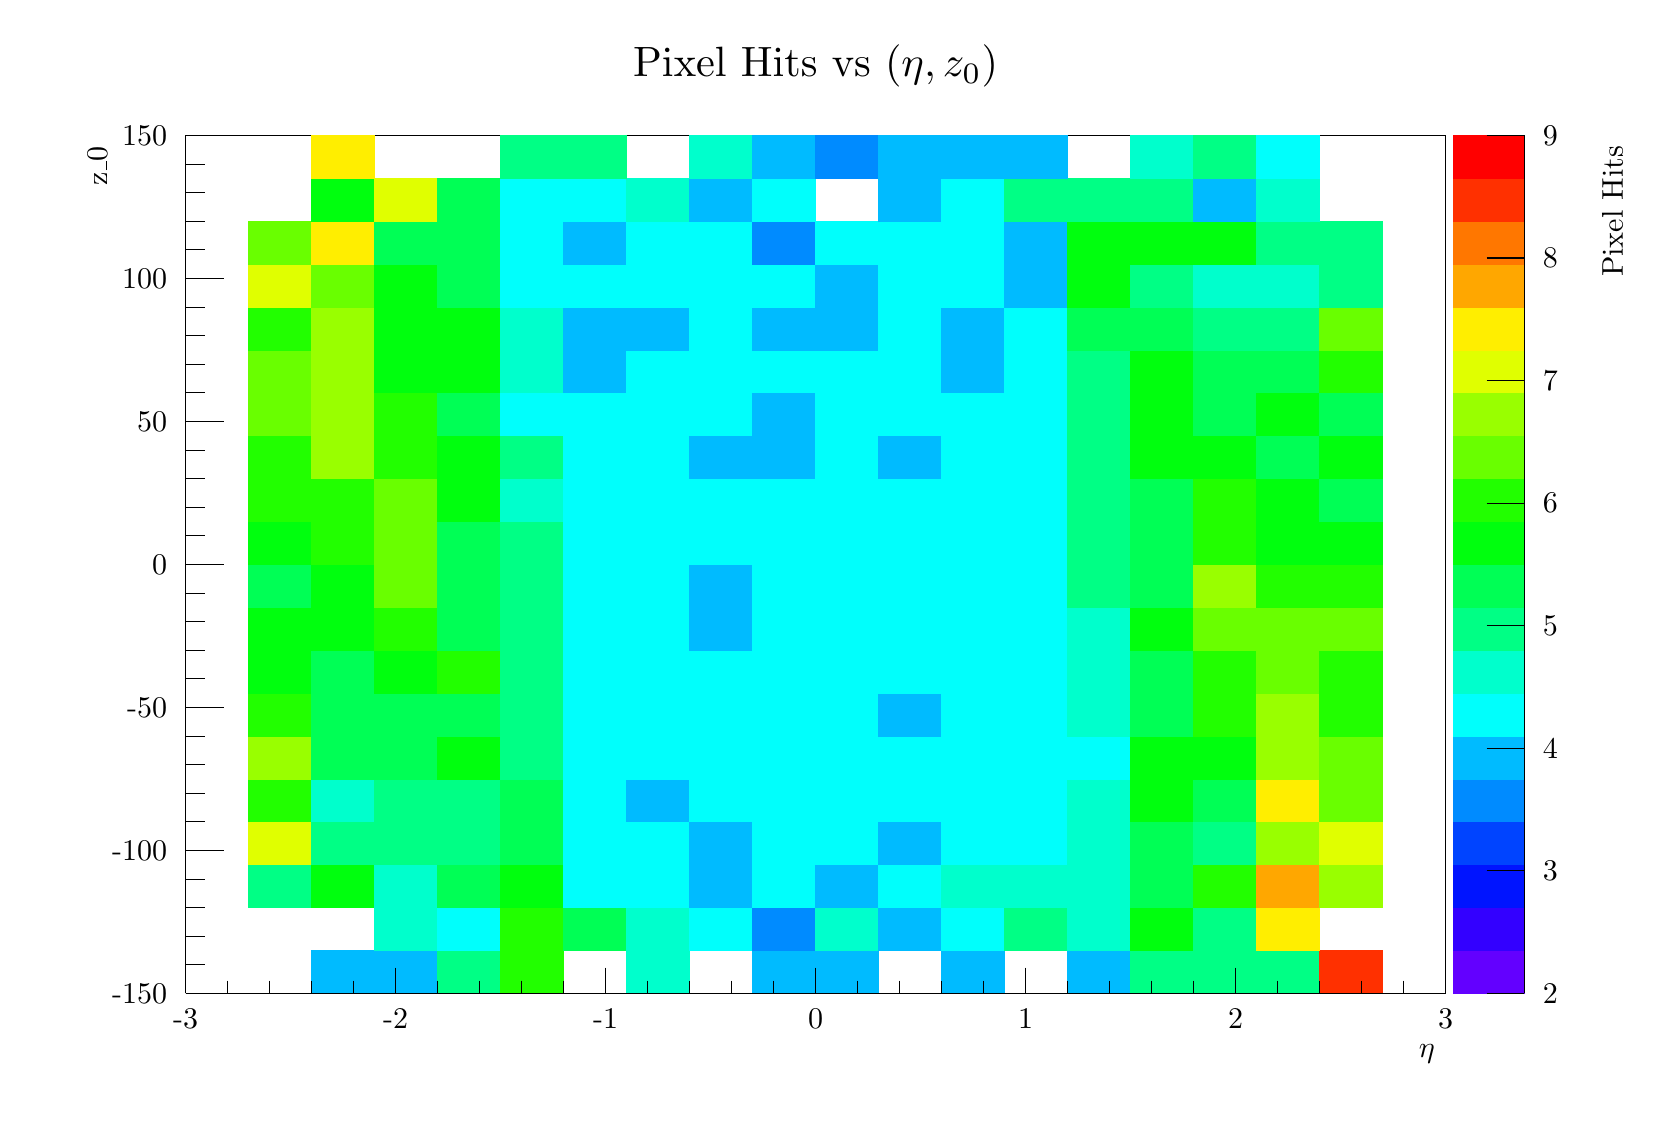
\begin{tikzpicture}
\pgfdeclareplotmark{cross} {
\pgfpathmoveto{\pgfpoint{-0.3\pgfplotmarksize}{\pgfplotmarksize}}
\pgfpathlineto{\pgfpoint{+0.3\pgfplotmarksize}{\pgfplotmarksize}}
\pgfpathlineto{\pgfpoint{+0.3\pgfplotmarksize}{0.3\pgfplotmarksize}}
\pgfpathlineto{\pgfpoint{+1\pgfplotmarksize}{0.3\pgfplotmarksize}}
\pgfpathlineto{\pgfpoint{+1\pgfplotmarksize}{-0.3\pgfplotmarksize}}
\pgfpathlineto{\pgfpoint{+0.3\pgfplotmarksize}{-0.3\pgfplotmarksize}}
\pgfpathlineto{\pgfpoint{+0.3\pgfplotmarksize}{-1.\pgfplotmarksize}}
\pgfpathlineto{\pgfpoint{-0.3\pgfplotmarksize}{-1.\pgfplotmarksize}}
\pgfpathlineto{\pgfpoint{-0.3\pgfplotmarksize}{-0.3\pgfplotmarksize}}
\pgfpathlineto{\pgfpoint{-1.\pgfplotmarksize}{-0.3\pgfplotmarksize}}
\pgfpathlineto{\pgfpoint{-1.\pgfplotmarksize}{0.3\pgfplotmarksize}}
\pgfpathlineto{\pgfpoint{-0.3\pgfplotmarksize}{0.3\pgfplotmarksize}}
\pgfpathclose
\pgfusepathqstroke
}
\pgfdeclareplotmark{cross*} {
\pgfpathmoveto{\pgfpoint{-0.3\pgfplotmarksize}{\pgfplotmarksize}}
\pgfpathlineto{\pgfpoint{+0.3\pgfplotmarksize}{\pgfplotmarksize}}
\pgfpathlineto{\pgfpoint{+0.3\pgfplotmarksize}{0.3\pgfplotmarksize}}
\pgfpathlineto{\pgfpoint{+1\pgfplotmarksize}{0.3\pgfplotmarksize}}
\pgfpathlineto{\pgfpoint{+1\pgfplotmarksize}{-0.3\pgfplotmarksize}}
\pgfpathlineto{\pgfpoint{+0.3\pgfplotmarksize}{-0.3\pgfplotmarksize}}
\pgfpathlineto{\pgfpoint{+0.3\pgfplotmarksize}{-1.\pgfplotmarksize}}
\pgfpathlineto{\pgfpoint{-0.3\pgfplotmarksize}{-1.\pgfplotmarksize}}
\pgfpathlineto{\pgfpoint{-0.3\pgfplotmarksize}{-0.3\pgfplotmarksize}}
\pgfpathlineto{\pgfpoint{-1.\pgfplotmarksize}{-0.3\pgfplotmarksize}}
\pgfpathlineto{\pgfpoint{-1.\pgfplotmarksize}{0.3\pgfplotmarksize}}
\pgfpathlineto{\pgfpoint{-0.3\pgfplotmarksize}{0.3\pgfplotmarksize}}
\pgfpathclose
\pgfusepathqfillstroke
}
\pgfdeclareplotmark{newstar} {
\pgfpathmoveto{\pgfqpoint{0pt}{\pgfplotmarksize}}
\pgfpathlineto{\pgfqpointpolar{44}{0.5\pgfplotmarksize}}
\pgfpathlineto{\pgfqpointpolar{18}{\pgfplotmarksize}}
\pgfpathlineto{\pgfqpointpolar{-20}{0.5\pgfplotmarksize}}
\pgfpathlineto{\pgfqpointpolar{-54}{\pgfplotmarksize}}
\pgfpathlineto{\pgfqpointpolar{-90}{0.5\pgfplotmarksize}}
\pgfpathlineto{\pgfqpointpolar{234}{\pgfplotmarksize}}
\pgfpathlineto{\pgfqpointpolar{198}{0.5\pgfplotmarksize}}
\pgfpathlineto{\pgfqpointpolar{162}{\pgfplotmarksize}}
\pgfpathlineto{\pgfqpointpolar{134}{0.5\pgfplotmarksize}}
\pgfpathclose
\pgfusepathqstroke
}
\pgfdeclareplotmark{newstar*} {
\pgfpathmoveto{\pgfqpoint{0pt}{\pgfplotmarksize}}
\pgfpathlineto{\pgfqpointpolar{44}{0.5\pgfplotmarksize}}
\pgfpathlineto{\pgfqpointpolar{18}{\pgfplotmarksize}}
\pgfpathlineto{\pgfqpointpolar{-20}{0.5\pgfplotmarksize}}
\pgfpathlineto{\pgfqpointpolar{-54}{\pgfplotmarksize}}
\pgfpathlineto{\pgfqpointpolar{-90}{0.5\pgfplotmarksize}}
\pgfpathlineto{\pgfqpointpolar{234}{\pgfplotmarksize}}
\pgfpathlineto{\pgfqpointpolar{198}{0.5\pgfplotmarksize}}
\pgfpathlineto{\pgfqpointpolar{162}{\pgfplotmarksize}}
\pgfpathlineto{\pgfqpointpolar{134}{0.5\pgfplotmarksize}}
\pgfpathclose
\pgfusepathqfillstroke
}
\definecolor{c}{rgb}{1,1,1};
\draw [color=c, fill=c] (0,0) rectangle (20,13.6207);
\draw [color=c, fill=c] (2,1.36207) rectangle (18,12.2586);
\definecolor{c}{rgb}{0,0,0};
\draw [c] (2,1.36207) -- (2,12.2586) -- (18,12.2586) -- (18,1.36207) -- (2,1.36207);
\definecolor{c}{rgb}{1,1,1};
\draw [color=c, fill=c] (2,1.36207) rectangle (18,12.2586);
\definecolor{c}{rgb}{0,0,0};
\draw [c] (2,1.36207) -- (2,12.2586) -- (18,12.2586) -- (18,1.36207) -- (2,1.36207);
\definecolor{c}{rgb}{0,0.733333,1};
\draw [color=c, fill=c] (3.6,1.36207) rectangle (4.4,1.9069);
\draw [color=c, fill=c] (4.4,1.36207) rectangle (5.2,1.9069);
\definecolor{c}{rgb}{0,1,0.52};
\draw [color=c, fill=c] (5.2,1.36207) rectangle (6,1.9069);
\definecolor{c}{rgb}{0.133333,1,0};
\draw [color=c, fill=c] (6,1.36207) rectangle (6.8,1.9069);
\definecolor{c}{rgb}{0,1,0.8};
\draw [color=c, fill=c] (7.6,1.36207) rectangle (8.4,1.9069);
\definecolor{c}{rgb}{0,0.733333,1};
\draw [color=c, fill=c] (9.2,1.36207) rectangle (10,1.9069);
\draw [color=c, fill=c] (10,1.36207) rectangle (10.8,1.9069);
\draw [color=c, fill=c] (11.6,1.36207) rectangle (12.4,1.9069);
\draw [color=c, fill=c] (13.2,1.36207) rectangle (14,1.9069);
\definecolor{c}{rgb}{0,1,0.52};
\draw [color=c, fill=c] (14,1.36207) rectangle (14.8,1.9069);
\draw [color=c, fill=c] (14.8,1.36207) rectangle (15.6,1.9069);
\draw [color=c, fill=c] (15.6,1.36207) rectangle (16.4,1.9069);
\definecolor{c}{rgb}{1,0.186667,0};
\draw [color=c, fill=c] (16.4,1.36207) rectangle (17.2,1.9069);
\definecolor{c}{rgb}{0,1,0.8};
\draw [color=c, fill=c] (4.4,1.9069) rectangle (5.2,2.45172);
\definecolor{c}{rgb}{0,1,0.986667};
\draw [color=c, fill=c] (5.2,1.9069) rectangle (6,2.45172);
\definecolor{c}{rgb}{0.133333,1,0};
\draw [color=c, fill=c] (6,1.9069) rectangle (6.8,2.45172);
\definecolor{c}{rgb}{0,1,0.333333};
\draw [color=c, fill=c] (6.8,1.9069) rectangle (7.6,2.45172);
\definecolor{c}{rgb}{0,1,0.8};
\draw [color=c, fill=c] (7.6,1.9069) rectangle (8.4,2.45172);
\definecolor{c}{rgb}{0,1,0.986667};
\draw [color=c, fill=c] (8.4,1.9069) rectangle (9.2,2.45172);
\definecolor{c}{rgb}{0,0.546666,1};
\draw [color=c, fill=c] (9.2,1.9069) rectangle (10,2.45172);
\definecolor{c}{rgb}{0,1,0.8};
\draw [color=c, fill=c] (10,1.9069) rectangle (10.8,2.45172);
\definecolor{c}{rgb}{0,0.733333,1};
\draw [color=c, fill=c] (10.8,1.9069) rectangle (11.6,2.45172);
\definecolor{c}{rgb}{0,1,0.986667};
\draw [color=c, fill=c] (11.6,1.9069) rectangle (12.4,2.45172);
\definecolor{c}{rgb}{0,1,0.52};
\draw [color=c, fill=c] (12.4,1.9069) rectangle (13.2,2.45172);
\definecolor{c}{rgb}{0,1,0.8};
\draw [color=c, fill=c] (13.2,1.9069) rectangle (14,2.45172);
\definecolor{c}{rgb}{0,1,0.0533333};
\draw [color=c, fill=c] (14,1.9069) rectangle (14.8,2.45172);
\definecolor{c}{rgb}{0,1,0.52};
\draw [color=c, fill=c] (14.8,1.9069) rectangle (15.6,2.45172);
\definecolor{c}{rgb}{1,0.933333,0};
\draw [color=c, fill=c] (15.6,1.9069) rectangle (16.4,2.45172);
\definecolor{c}{rgb}{0,1,0.52};
\draw [color=c, fill=c] (2.8,2.45172) rectangle (3.6,2.99655);
\definecolor{c}{rgb}{0,1,0.0533333};
\draw [color=c, fill=c] (3.6,2.45172) rectangle (4.4,2.99655);
\definecolor{c}{rgb}{0,1,0.8};
\draw [color=c, fill=c] (4.4,2.45172) rectangle (5.2,2.99655);
\definecolor{c}{rgb}{0,1,0.333333};
\draw [color=c, fill=c] (5.2,2.45172) rectangle (6,2.99655);
\definecolor{c}{rgb}{0,1,0.0533333};
\draw [color=c, fill=c] (6,2.45172) rectangle (6.8,2.99655);
\definecolor{c}{rgb}{0,1,0.986667};
\draw [color=c, fill=c] (6.8,2.45172) rectangle (7.6,2.99655);
\draw [color=c, fill=c] (7.6,2.45172) rectangle (8.4,2.99655);
\definecolor{c}{rgb}{0,0.733333,1};
\draw [color=c, fill=c] (8.4,2.45172) rectangle (9.2,2.99655);
\definecolor{c}{rgb}{0,1,0.986667};
\draw [color=c, fill=c] (9.2,2.45172) rectangle (10,2.99655);
\definecolor{c}{rgb}{0,0.733333,1};
\draw [color=c, fill=c] (10,2.45172) rectangle (10.8,2.99655);
\definecolor{c}{rgb}{0,1,0.986667};
\draw [color=c, fill=c] (10.8,2.45172) rectangle (11.6,2.99655);
\definecolor{c}{rgb}{0,1,0.8};
\draw [color=c, fill=c] (11.6,2.45172) rectangle (12.4,2.99655);
\draw [color=c, fill=c] (12.4,2.45172) rectangle (13.2,2.99655);
\draw [color=c, fill=c] (13.2,2.45172) rectangle (14,2.99655);
\definecolor{c}{rgb}{0,1,0.333333};
\draw [color=c, fill=c] (14,2.45172) rectangle (14.8,2.99655);
\definecolor{c}{rgb}{0.133333,1,0};
\draw [color=c, fill=c] (14.8,2.45172) rectangle (15.6,2.99655);
\definecolor{c}{rgb}{1,0.653333,0};
\draw [color=c, fill=c] (15.6,2.45172) rectangle (16.4,2.99655);
\definecolor{c}{rgb}{0.6,1,0};
\draw [color=c, fill=c] (16.4,2.45172) rectangle (17.2,2.99655);
\definecolor{c}{rgb}{0.88,1,0};
\draw [color=c, fill=c] (2.8,2.99655) rectangle (3.6,3.54138);
\definecolor{c}{rgb}{0,1,0.52};
\draw [color=c, fill=c] (3.6,2.99655) rectangle (4.4,3.54138);
\draw [color=c, fill=c] (4.4,2.99655) rectangle (5.2,3.54138);
\draw [color=c, fill=c] (5.2,2.99655) rectangle (6,3.54138);
\definecolor{c}{rgb}{0,1,0.333333};
\draw [color=c, fill=c] (6,2.99655) rectangle (6.8,3.54138);
\definecolor{c}{rgb}{0,1,0.986667};
\draw [color=c, fill=c] (6.8,2.99655) rectangle (7.6,3.54138);
\draw [color=c, fill=c] (7.6,2.99655) rectangle (8.4,3.54138);
\definecolor{c}{rgb}{0,0.733333,1};
\draw [color=c, fill=c] (8.4,2.99655) rectangle (9.2,3.54138);
\definecolor{c}{rgb}{0,1,0.986667};
\draw [color=c, fill=c] (9.2,2.99655) rectangle (10,3.54138);
\draw [color=c, fill=c] (10,2.99655) rectangle (10.8,3.54138);
\definecolor{c}{rgb}{0,0.733333,1};
\draw [color=c, fill=c] (10.8,2.99655) rectangle (11.6,3.54138);
\definecolor{c}{rgb}{0,1,0.986667};
\draw [color=c, fill=c] (11.6,2.99655) rectangle (12.4,3.54138);
\draw [color=c, fill=c] (12.4,2.99655) rectangle (13.2,3.54138);
\definecolor{c}{rgb}{0,1,0.8};
\draw [color=c, fill=c] (13.2,2.99655) rectangle (14,3.54138);
\definecolor{c}{rgb}{0,1,0.333333};
\draw [color=c, fill=c] (14,2.99655) rectangle (14.8,3.54138);
\definecolor{c}{rgb}{0,1,0.52};
\draw [color=c, fill=c] (14.8,2.99655) rectangle (15.6,3.54138);
\definecolor{c}{rgb}{0.6,1,0};
\draw [color=c, fill=c] (15.6,2.99655) rectangle (16.4,3.54138);
\definecolor{c}{rgb}{0.88,1,0};
\draw [color=c, fill=c] (16.4,2.99655) rectangle (17.2,3.54138);
\definecolor{c}{rgb}{0.133333,1,0};
\draw [color=c, fill=c] (2.8,3.54138) rectangle (3.6,4.08621);
\definecolor{c}{rgb}{0,1,0.8};
\draw [color=c, fill=c] (3.6,3.54138) rectangle (4.4,4.08621);
\definecolor{c}{rgb}{0,1,0.52};
\draw [color=c, fill=c] (4.4,3.54138) rectangle (5.2,4.08621);
\draw [color=c, fill=c] (5.2,3.54138) rectangle (6,4.08621);
\definecolor{c}{rgb}{0,1,0.333333};
\draw [color=c, fill=c] (6,3.54138) rectangle (6.8,4.08621);
\definecolor{c}{rgb}{0,1,0.986667};
\draw [color=c, fill=c] (6.8,3.54138) rectangle (7.6,4.08621);
\definecolor{c}{rgb}{0,0.733333,1};
\draw [color=c, fill=c] (7.6,3.54138) rectangle (8.4,4.08621);
\definecolor{c}{rgb}{0,1,0.986667};
\draw [color=c, fill=c] (8.4,3.54138) rectangle (9.2,4.08621);
\draw [color=c, fill=c] (9.2,3.54138) rectangle (10,4.08621);
\draw [color=c, fill=c] (10,3.54138) rectangle (10.8,4.08621);
\draw [color=c, fill=c] (10.8,3.54138) rectangle (11.6,4.08621);
\draw [color=c, fill=c] (11.6,3.54138) rectangle (12.4,4.08621);
\draw [color=c, fill=c] (12.4,3.54138) rectangle (13.2,4.08621);
\definecolor{c}{rgb}{0,1,0.8};
\draw [color=c, fill=c] (13.2,3.54138) rectangle (14,4.08621);
\definecolor{c}{rgb}{0,1,0.0533333};
\draw [color=c, fill=c] (14,3.54138) rectangle (14.8,4.08621);
\definecolor{c}{rgb}{0,1,0.333333};
\draw [color=c, fill=c] (14.8,3.54138) rectangle (15.6,4.08621);
\definecolor{c}{rgb}{1,0.933333,0};
\draw [color=c, fill=c] (15.6,3.54138) rectangle (16.4,4.08621);
\definecolor{c}{rgb}{0.413333,1,0};
\draw [color=c, fill=c] (16.4,3.54138) rectangle (17.2,4.08621);
\definecolor{c}{rgb}{0.6,1,0};
\draw [color=c, fill=c] (2.8,4.08621) rectangle (3.6,4.63103);
\definecolor{c}{rgb}{0,1,0.333333};
\draw [color=c, fill=c] (3.6,4.08621) rectangle (4.4,4.63103);
\draw [color=c, fill=c] (4.4,4.08621) rectangle (5.2,4.63103);
\definecolor{c}{rgb}{0,1,0.0533333};
\draw [color=c, fill=c] (5.2,4.08621) rectangle (6,4.63103);
\definecolor{c}{rgb}{0,1,0.52};
\draw [color=c, fill=c] (6,4.08621) rectangle (6.8,4.63103);
\definecolor{c}{rgb}{0,1,0.986667};
\draw [color=c, fill=c] (6.8,4.08621) rectangle (7.6,4.63103);
\draw [color=c, fill=c] (7.6,4.08621) rectangle (8.4,4.63103);
\draw [color=c, fill=c] (8.4,4.08621) rectangle (9.2,4.63103);
\draw [color=c, fill=c] (9.2,4.08621) rectangle (10,4.63103);
\draw [color=c, fill=c] (10,4.08621) rectangle (10.8,4.63103);
\draw [color=c, fill=c] (10.8,4.08621) rectangle (11.6,4.63103);
\draw [color=c, fill=c] (11.6,4.08621) rectangle (12.4,4.63103);
\draw [color=c, fill=c] (12.4,4.08621) rectangle (13.2,4.63103);
\draw [color=c, fill=c] (13.2,4.08621) rectangle (14,4.63103);
\definecolor{c}{rgb}{0,1,0.0533333};
\draw [color=c, fill=c] (14,4.08621) rectangle (14.8,4.63103);
\draw [color=c, fill=c] (14.8,4.08621) rectangle (15.6,4.63103);
\definecolor{c}{rgb}{0.6,1,0};
\draw [color=c, fill=c] (15.6,4.08621) rectangle (16.4,4.63103);
\definecolor{c}{rgb}{0.413333,1,0};
\draw [color=c, fill=c] (16.4,4.08621) rectangle (17.2,4.63103);
\definecolor{c}{rgb}{0.133333,1,0};
\draw [color=c, fill=c] (2.8,4.63103) rectangle (3.6,5.17586);
\definecolor{c}{rgb}{0,1,0.333333};
\draw [color=c, fill=c] (3.6,4.63103) rectangle (4.4,5.17586);
\draw [color=c, fill=c] (4.4,4.63103) rectangle (5.2,5.17586);
\draw [color=c, fill=c] (5.2,4.63103) rectangle (6,5.17586);
\definecolor{c}{rgb}{0,1,0.52};
\draw [color=c, fill=c] (6,4.63103) rectangle (6.8,5.17586);
\definecolor{c}{rgb}{0,1,0.986667};
\draw [color=c, fill=c] (6.8,4.63103) rectangle (7.6,5.17586);
\draw [color=c, fill=c] (7.6,4.63103) rectangle (8.4,5.17586);
\draw [color=c, fill=c] (8.4,4.63103) rectangle (9.2,5.17586);
\draw [color=c, fill=c] (9.2,4.63103) rectangle (10,5.17586);
\draw [color=c, fill=c] (10,4.63103) rectangle (10.8,5.17586);
\definecolor{c}{rgb}{0,0.733333,1};
\draw [color=c, fill=c] (10.8,4.63103) rectangle (11.6,5.17586);
\definecolor{c}{rgb}{0,1,0.986667};
\draw [color=c, fill=c] (11.6,4.63103) rectangle (12.4,5.17586);
\draw [color=c, fill=c] (12.4,4.63103) rectangle (13.2,5.17586);
\definecolor{c}{rgb}{0,1,0.8};
\draw [color=c, fill=c] (13.2,4.63103) rectangle (14,5.17586);
\definecolor{c}{rgb}{0,1,0.333333};
\draw [color=c, fill=c] (14,4.63103) rectangle (14.8,5.17586);
\definecolor{c}{rgb}{0.133333,1,0};
\draw [color=c, fill=c] (14.8,4.63103) rectangle (15.6,5.17586);
\definecolor{c}{rgb}{0.6,1,0};
\draw [color=c, fill=c] (15.6,4.63103) rectangle (16.4,5.17586);
\definecolor{c}{rgb}{0.133333,1,0};
\draw [color=c, fill=c] (16.4,4.63103) rectangle (17.2,5.17586);
\definecolor{c}{rgb}{0,1,0.0533333};
\draw [color=c, fill=c] (2.8,5.17586) rectangle (3.6,5.72069);
\definecolor{c}{rgb}{0,1,0.333333};
\draw [color=c, fill=c] (3.6,5.17586) rectangle (4.4,5.72069);
\definecolor{c}{rgb}{0,1,0.0533333};
\draw [color=c, fill=c] (4.4,5.17586) rectangle (5.2,5.72069);
\definecolor{c}{rgb}{0.133333,1,0};
\draw [color=c, fill=c] (5.2,5.17586) rectangle (6,5.72069);
\definecolor{c}{rgb}{0,1,0.52};
\draw [color=c, fill=c] (6,5.17586) rectangle (6.8,5.72069);
\definecolor{c}{rgb}{0,1,0.986667};
\draw [color=c, fill=c] (6.8,5.17586) rectangle (7.6,5.72069);
\draw [color=c, fill=c] (7.6,5.17586) rectangle (8.4,5.72069);
\draw [color=c, fill=c] (8.4,5.17586) rectangle (9.2,5.72069);
\draw [color=c, fill=c] (9.2,5.17586) rectangle (10,5.72069);
\draw [color=c, fill=c] (10,5.17586) rectangle (10.8,5.72069);
\draw [color=c, fill=c] (10.8,5.17586) rectangle (11.6,5.72069);
\draw [color=c, fill=c] (11.6,5.17586) rectangle (12.4,5.72069);
\draw [color=c, fill=c] (12.4,5.17586) rectangle (13.2,5.72069);
\definecolor{c}{rgb}{0,1,0.8};
\draw [color=c, fill=c] (13.2,5.17586) rectangle (14,5.72069);
\definecolor{c}{rgb}{0,1,0.333333};
\draw [color=c, fill=c] (14,5.17586) rectangle (14.8,5.72069);
\definecolor{c}{rgb}{0.133333,1,0};
\draw [color=c, fill=c] (14.8,5.17586) rectangle (15.6,5.72069);
\definecolor{c}{rgb}{0.413333,1,0};
\draw [color=c, fill=c] (15.6,5.17586) rectangle (16.4,5.72069);
\definecolor{c}{rgb}{0.133333,1,0};
\draw [color=c, fill=c] (16.4,5.17586) rectangle (17.2,5.72069);
\definecolor{c}{rgb}{0,1,0.0533333};
\draw [color=c, fill=c] (2.8,5.72069) rectangle (3.6,6.26552);
\draw [color=c, fill=c] (3.6,5.72069) rectangle (4.4,6.26552);
\definecolor{c}{rgb}{0.133333,1,0};
\draw [color=c, fill=c] (4.4,5.72069) rectangle (5.2,6.26552);
\definecolor{c}{rgb}{0,1,0.333333};
\draw [color=c, fill=c] (5.2,5.72069) rectangle (6,6.26552);
\definecolor{c}{rgb}{0,1,0.52};
\draw [color=c, fill=c] (6,5.72069) rectangle (6.8,6.26552);
\definecolor{c}{rgb}{0,1,0.986667};
\draw [color=c, fill=c] (6.8,5.72069) rectangle (7.6,6.26552);
\draw [color=c, fill=c] (7.6,5.72069) rectangle (8.4,6.26552);
\definecolor{c}{rgb}{0,0.733333,1};
\draw [color=c, fill=c] (8.4,5.72069) rectangle (9.2,6.26552);
\definecolor{c}{rgb}{0,1,0.986667};
\draw [color=c, fill=c] (9.2,5.72069) rectangle (10,6.26552);
\draw [color=c, fill=c] (10,5.72069) rectangle (10.8,6.26552);
\draw [color=c, fill=c] (10.8,5.72069) rectangle (11.6,6.26552);
\draw [color=c, fill=c] (11.6,5.72069) rectangle (12.4,6.26552);
\draw [color=c, fill=c] (12.4,5.72069) rectangle (13.2,6.26552);
\definecolor{c}{rgb}{0,1,0.8};
\draw [color=c, fill=c] (13.2,5.72069) rectangle (14,6.26552);
\definecolor{c}{rgb}{0,1,0.0533333};
\draw [color=c, fill=c] (14,5.72069) rectangle (14.8,6.26552);
\definecolor{c}{rgb}{0.413333,1,0};
\draw [color=c, fill=c] (14.8,5.72069) rectangle (15.6,6.26552);
\draw [color=c, fill=c] (15.6,5.72069) rectangle (16.4,6.26552);
\draw [color=c, fill=c] (16.4,5.72069) rectangle (17.2,6.26552);
\definecolor{c}{rgb}{0,1,0.333333};
\draw [color=c, fill=c] (2.8,6.26552) rectangle (3.6,6.81034);
\definecolor{c}{rgb}{0,1,0.0533333};
\draw [color=c, fill=c] (3.6,6.26552) rectangle (4.4,6.81034);
\definecolor{c}{rgb}{0.413333,1,0};
\draw [color=c, fill=c] (4.4,6.26552) rectangle (5.2,6.81034);
\definecolor{c}{rgb}{0,1,0.333333};
\draw [color=c, fill=c] (5.2,6.26552) rectangle (6,6.81034);
\definecolor{c}{rgb}{0,1,0.52};
\draw [color=c, fill=c] (6,6.26552) rectangle (6.8,6.81034);
\definecolor{c}{rgb}{0,1,0.986667};
\draw [color=c, fill=c] (6.8,6.26552) rectangle (7.6,6.81034);
\draw [color=c, fill=c] (7.6,6.26552) rectangle (8.4,6.81034);
\definecolor{c}{rgb}{0,0.733333,1};
\draw [color=c, fill=c] (8.4,6.26552) rectangle (9.2,6.81034);
\definecolor{c}{rgb}{0,1,0.986667};
\draw [color=c, fill=c] (9.2,6.26552) rectangle (10,6.81034);
\draw [color=c, fill=c] (10,6.26552) rectangle (10.8,6.81034);
\draw [color=c, fill=c] (10.8,6.26552) rectangle (11.6,6.81034);
\draw [color=c, fill=c] (11.6,6.26552) rectangle (12.4,6.81034);
\draw [color=c, fill=c] (12.4,6.26552) rectangle (13.2,6.81034);
\definecolor{c}{rgb}{0,1,0.52};
\draw [color=c, fill=c] (13.2,6.26552) rectangle (14,6.81034);
\definecolor{c}{rgb}{0,1,0.333333};
\draw [color=c, fill=c] (14,6.26552) rectangle (14.8,6.81034);
\definecolor{c}{rgb}{0.6,1,0};
\draw [color=c, fill=c] (14.8,6.26552) rectangle (15.6,6.81034);
\definecolor{c}{rgb}{0.133333,1,0};
\draw [color=c, fill=c] (15.6,6.26552) rectangle (16.4,6.81034);
\draw [color=c, fill=c] (16.4,6.26552) rectangle (17.2,6.81034);
\definecolor{c}{rgb}{0,1,0.0533333};
\draw [color=c, fill=c] (2.8,6.81034) rectangle (3.6,7.35517);
\definecolor{c}{rgb}{0.133333,1,0};
\draw [color=c, fill=c] (3.6,6.81034) rectangle (4.4,7.35517);
\definecolor{c}{rgb}{0.413333,1,0};
\draw [color=c, fill=c] (4.4,6.81034) rectangle (5.2,7.35517);
\definecolor{c}{rgb}{0,1,0.333333};
\draw [color=c, fill=c] (5.2,6.81034) rectangle (6,7.35517);
\definecolor{c}{rgb}{0,1,0.52};
\draw [color=c, fill=c] (6,6.81034) rectangle (6.8,7.35517);
\definecolor{c}{rgb}{0,1,0.986667};
\draw [color=c, fill=c] (6.8,6.81034) rectangle (7.6,7.35517);
\draw [color=c, fill=c] (7.6,6.81034) rectangle (8.4,7.35517);
\draw [color=c, fill=c] (8.4,6.81034) rectangle (9.2,7.35517);
\draw [color=c, fill=c] (9.2,6.81034) rectangle (10,7.35517);
\draw [color=c, fill=c] (10,6.81034) rectangle (10.8,7.35517);
\draw [color=c, fill=c] (10.8,6.81034) rectangle (11.6,7.35517);
\draw [color=c, fill=c] (11.6,6.81034) rectangle (12.4,7.35517);
\draw [color=c, fill=c] (12.4,6.81034) rectangle (13.2,7.35517);
\definecolor{c}{rgb}{0,1,0.52};
\draw [color=c, fill=c] (13.2,6.81034) rectangle (14,7.35517);
\definecolor{c}{rgb}{0,1,0.333333};
\draw [color=c, fill=c] (14,6.81034) rectangle (14.8,7.35517);
\definecolor{c}{rgb}{0.133333,1,0};
\draw [color=c, fill=c] (14.8,6.81034) rectangle (15.6,7.35517);
\definecolor{c}{rgb}{0,1,0.0533333};
\draw [color=c, fill=c] (15.6,6.81034) rectangle (16.4,7.35517);
\draw [color=c, fill=c] (16.4,6.81034) rectangle (17.2,7.35517);
\definecolor{c}{rgb}{0.133333,1,0};
\draw [color=c, fill=c] (2.8,7.35517) rectangle (3.6,7.9);
\draw [color=c, fill=c] (3.6,7.35517) rectangle (4.4,7.9);
\definecolor{c}{rgb}{0.413333,1,0};
\draw [color=c, fill=c] (4.4,7.35517) rectangle (5.2,7.9);
\definecolor{c}{rgb}{0,1,0.0533333};
\draw [color=c, fill=c] (5.2,7.35517) rectangle (6,7.9);
\definecolor{c}{rgb}{0,1,0.8};
\draw [color=c, fill=c] (6,7.35517) rectangle (6.8,7.9);
\definecolor{c}{rgb}{0,1,0.986667};
\draw [color=c, fill=c] (6.8,7.35517) rectangle (7.6,7.9);
\draw [color=c, fill=c] (7.6,7.35517) rectangle (8.4,7.9);
\draw [color=c, fill=c] (8.4,7.35517) rectangle (9.2,7.9);
\draw [color=c, fill=c] (9.2,7.35517) rectangle (10,7.9);
\draw [color=c, fill=c] (10,7.35517) rectangle (10.8,7.9);
\draw [color=c, fill=c] (10.8,7.35517) rectangle (11.6,7.9);
\draw [color=c, fill=c] (11.6,7.35517) rectangle (12.4,7.9);
\draw [color=c, fill=c] (12.4,7.35517) rectangle (13.2,7.9);
\definecolor{c}{rgb}{0,1,0.52};
\draw [color=c, fill=c] (13.2,7.35517) rectangle (14,7.9);
\definecolor{c}{rgb}{0,1,0.333333};
\draw [color=c, fill=c] (14,7.35517) rectangle (14.8,7.9);
\definecolor{c}{rgb}{0.133333,1,0};
\draw [color=c, fill=c] (14.8,7.35517) rectangle (15.6,7.9);
\definecolor{c}{rgb}{0,1,0.0533333};
\draw [color=c, fill=c] (15.6,7.35517) rectangle (16.4,7.9);
\definecolor{c}{rgb}{0,1,0.333333};
\draw [color=c, fill=c] (16.4,7.35517) rectangle (17.2,7.9);
\definecolor{c}{rgb}{0.133333,1,0};
\draw [color=c, fill=c] (2.8,7.9) rectangle (3.6,8.44483);
\definecolor{c}{rgb}{0.6,1,0};
\draw [color=c, fill=c] (3.6,7.9) rectangle (4.4,8.44483);
\definecolor{c}{rgb}{0.133333,1,0};
\draw [color=c, fill=c] (4.4,7.9) rectangle (5.2,8.44483);
\definecolor{c}{rgb}{0,1,0.0533333};
\draw [color=c, fill=c] (5.2,7.9) rectangle (6,8.44483);
\definecolor{c}{rgb}{0,1,0.52};
\draw [color=c, fill=c] (6,7.9) rectangle (6.8,8.44483);
\definecolor{c}{rgb}{0,1,0.986667};
\draw [color=c, fill=c] (6.8,7.9) rectangle (7.6,8.44483);
\draw [color=c, fill=c] (7.6,7.9) rectangle (8.4,8.44483);
\definecolor{c}{rgb}{0,0.733333,1};
\draw [color=c, fill=c] (8.4,7.9) rectangle (9.2,8.44483);
\draw [color=c, fill=c] (9.2,7.9) rectangle (10,8.44483);
\definecolor{c}{rgb}{0,1,0.986667};
\draw [color=c, fill=c] (10,7.9) rectangle (10.8,8.44483);
\definecolor{c}{rgb}{0,0.733333,1};
\draw [color=c, fill=c] (10.8,7.9) rectangle (11.6,8.44483);
\definecolor{c}{rgb}{0,1,0.986667};
\draw [color=c, fill=c] (11.6,7.9) rectangle (12.4,8.44483);
\draw [color=c, fill=c] (12.4,7.9) rectangle (13.2,8.44483);
\definecolor{c}{rgb}{0,1,0.52};
\draw [color=c, fill=c] (13.2,7.9) rectangle (14,8.44483);
\definecolor{c}{rgb}{0,1,0.0533333};
\draw [color=c, fill=c] (14,7.9) rectangle (14.8,8.44483);
\draw [color=c, fill=c] (14.8,7.9) rectangle (15.6,8.44483);
\definecolor{c}{rgb}{0,1,0.333333};
\draw [color=c, fill=c] (15.6,7.9) rectangle (16.4,8.44483);
\definecolor{c}{rgb}{0,1,0.0533333};
\draw [color=c, fill=c] (16.4,7.9) rectangle (17.2,8.44483);
\definecolor{c}{rgb}{0.413333,1,0};
\draw [color=c, fill=c] (2.8,8.44483) rectangle (3.6,8.98965);
\definecolor{c}{rgb}{0.6,1,0};
\draw [color=c, fill=c] (3.6,8.44483) rectangle (4.4,8.98965);
\definecolor{c}{rgb}{0.133333,1,0};
\draw [color=c, fill=c] (4.4,8.44483) rectangle (5.2,8.98965);
\definecolor{c}{rgb}{0,1,0.333333};
\draw [color=c, fill=c] (5.2,8.44483) rectangle (6,8.98965);
\definecolor{c}{rgb}{0,1,0.986667};
\draw [color=c, fill=c] (6,8.44483) rectangle (6.8,8.98965);
\draw [color=c, fill=c] (6.8,8.44483) rectangle (7.6,8.98965);
\draw [color=c, fill=c] (7.6,8.44483) rectangle (8.4,8.98965);
\draw [color=c, fill=c] (8.4,8.44483) rectangle (9.2,8.98965);
\definecolor{c}{rgb}{0,0.733333,1};
\draw [color=c, fill=c] (9.2,8.44483) rectangle (10,8.98965);
\definecolor{c}{rgb}{0,1,0.986667};
\draw [color=c, fill=c] (10,8.44483) rectangle (10.8,8.98965);
\draw [color=c, fill=c] (10.8,8.44483) rectangle (11.6,8.98965);
\draw [color=c, fill=c] (11.6,8.44483) rectangle (12.4,8.98965);
\draw [color=c, fill=c] (12.4,8.44483) rectangle (13.2,8.98965);
\definecolor{c}{rgb}{0,1,0.52};
\draw [color=c, fill=c] (13.2,8.44483) rectangle (14,8.98965);
\definecolor{c}{rgb}{0,1,0.0533333};
\draw [color=c, fill=c] (14,8.44483) rectangle (14.8,8.98965);
\definecolor{c}{rgb}{0,1,0.333333};
\draw [color=c, fill=c] (14.8,8.44483) rectangle (15.6,8.98965);
\definecolor{c}{rgb}{0,1,0.0533333};
\draw [color=c, fill=c] (15.6,8.44483) rectangle (16.4,8.98965);
\definecolor{c}{rgb}{0,1,0.333333};
\draw [color=c, fill=c] (16.4,8.44483) rectangle (17.2,8.98965);
\definecolor{c}{rgb}{0.413333,1,0};
\draw [color=c, fill=c] (2.8,8.98965) rectangle (3.6,9.53448);
\definecolor{c}{rgb}{0.6,1,0};
\draw [color=c, fill=c] (3.6,8.98965) rectangle (4.4,9.53448);
\definecolor{c}{rgb}{0,1,0.0533333};
\draw [color=c, fill=c] (4.4,8.98965) rectangle (5.2,9.53448);
\draw [color=c, fill=c] (5.2,8.98965) rectangle (6,9.53448);
\definecolor{c}{rgb}{0,1,0.8};
\draw [color=c, fill=c] (6,8.98965) rectangle (6.8,9.53448);
\definecolor{c}{rgb}{0,0.733333,1};
\draw [color=c, fill=c] (6.8,8.98965) rectangle (7.6,9.53448);
\definecolor{c}{rgb}{0,1,0.986667};
\draw [color=c, fill=c] (7.6,8.98965) rectangle (8.4,9.53448);
\draw [color=c, fill=c] (8.4,8.98965) rectangle (9.2,9.53448);
\draw [color=c, fill=c] (9.2,8.98965) rectangle (10,9.53448);
\draw [color=c, fill=c] (10,8.98965) rectangle (10.8,9.53448);
\draw [color=c, fill=c] (10.8,8.98965) rectangle (11.6,9.53448);
\definecolor{c}{rgb}{0,0.733333,1};
\draw [color=c, fill=c] (11.6,8.98965) rectangle (12.4,9.53448);
\definecolor{c}{rgb}{0,1,0.986667};
\draw [color=c, fill=c] (12.4,8.98965) rectangle (13.2,9.53448);
\definecolor{c}{rgb}{0,1,0.52};
\draw [color=c, fill=c] (13.2,8.98965) rectangle (14,9.53448);
\definecolor{c}{rgb}{0,1,0.0533333};
\draw [color=c, fill=c] (14,8.98965) rectangle (14.8,9.53448);
\definecolor{c}{rgb}{0,1,0.333333};
\draw [color=c, fill=c] (14.8,8.98965) rectangle (15.6,9.53448);
\draw [color=c, fill=c] (15.6,8.98965) rectangle (16.4,9.53448);
\definecolor{c}{rgb}{0.133333,1,0};
\draw [color=c, fill=c] (16.4,8.98965) rectangle (17.2,9.53448);
\draw [color=c, fill=c] (2.8,9.53448) rectangle (3.6,10.0793);
\definecolor{c}{rgb}{0.6,1,0};
\draw [color=c, fill=c] (3.6,9.53448) rectangle (4.4,10.0793);
\definecolor{c}{rgb}{0,1,0.0533333};
\draw [color=c, fill=c] (4.4,9.53448) rectangle (5.2,10.0793);
\draw [color=c, fill=c] (5.2,9.53448) rectangle (6,10.0793);
\definecolor{c}{rgb}{0,1,0.8};
\draw [color=c, fill=c] (6,9.53448) rectangle (6.8,10.0793);
\definecolor{c}{rgb}{0,0.733333,1};
\draw [color=c, fill=c] (6.8,9.53448) rectangle (7.6,10.0793);
\draw [color=c, fill=c] (7.6,9.53448) rectangle (8.4,10.0793);
\definecolor{c}{rgb}{0,1,0.986667};
\draw [color=c, fill=c] (8.4,9.53448) rectangle (9.2,10.0793);
\definecolor{c}{rgb}{0,0.733333,1};
\draw [color=c, fill=c] (9.2,9.53448) rectangle (10,10.0793);
\draw [color=c, fill=c] (10,9.53448) rectangle (10.8,10.0793);
\definecolor{c}{rgb}{0,1,0.986667};
\draw [color=c, fill=c] (10.8,9.53448) rectangle (11.6,10.0793);
\definecolor{c}{rgb}{0,0.733333,1};
\draw [color=c, fill=c] (11.6,9.53448) rectangle (12.4,10.0793);
\definecolor{c}{rgb}{0,1,0.986667};
\draw [color=c, fill=c] (12.4,9.53448) rectangle (13.2,10.0793);
\definecolor{c}{rgb}{0,1,0.333333};
\draw [color=c, fill=c] (13.2,9.53448) rectangle (14,10.0793);
\draw [color=c, fill=c] (14,9.53448) rectangle (14.8,10.0793);
\definecolor{c}{rgb}{0,1,0.52};
\draw [color=c, fill=c] (14.8,9.53448) rectangle (15.6,10.0793);
\draw [color=c, fill=c] (15.6,9.53448) rectangle (16.4,10.0793);
\definecolor{c}{rgb}{0.413333,1,0};
\draw [color=c, fill=c] (16.4,9.53448) rectangle (17.2,10.0793);
\definecolor{c}{rgb}{0.88,1,0};
\draw [color=c, fill=c] (2.8,10.0793) rectangle (3.6,10.6241);
\definecolor{c}{rgb}{0.413333,1,0};
\draw [color=c, fill=c] (3.6,10.0793) rectangle (4.4,10.6241);
\definecolor{c}{rgb}{0,1,0.0533333};
\draw [color=c, fill=c] (4.4,10.0793) rectangle (5.2,10.6241);
\definecolor{c}{rgb}{0,1,0.333333};
\draw [color=c, fill=c] (5.2,10.0793) rectangle (6,10.6241);
\definecolor{c}{rgb}{0,1,0.986667};
\draw [color=c, fill=c] (6,10.0793) rectangle (6.8,10.6241);
\draw [color=c, fill=c] (6.8,10.0793) rectangle (7.6,10.6241);
\draw [color=c, fill=c] (7.6,10.0793) rectangle (8.4,10.6241);
\draw [color=c, fill=c] (8.4,10.0793) rectangle (9.2,10.6241);
\draw [color=c, fill=c] (9.2,10.0793) rectangle (10,10.6241);
\definecolor{c}{rgb}{0,0.733333,1};
\draw [color=c, fill=c] (10,10.0793) rectangle (10.8,10.6241);
\definecolor{c}{rgb}{0,1,0.986667};
\draw [color=c, fill=c] (10.8,10.0793) rectangle (11.6,10.6241);
\draw [color=c, fill=c] (11.6,10.0793) rectangle (12.4,10.6241);
\definecolor{c}{rgb}{0,0.733333,1};
\draw [color=c, fill=c] (12.4,10.0793) rectangle (13.2,10.6241);
\definecolor{c}{rgb}{0,1,0.0533333};
\draw [color=c, fill=c] (13.2,10.0793) rectangle (14,10.6241);
\definecolor{c}{rgb}{0,1,0.52};
\draw [color=c, fill=c] (14,10.0793) rectangle (14.8,10.6241);
\definecolor{c}{rgb}{0,1,0.8};
\draw [color=c, fill=c] (14.8,10.0793) rectangle (15.6,10.6241);
\draw [color=c, fill=c] (15.6,10.0793) rectangle (16.4,10.6241);
\definecolor{c}{rgb}{0,1,0.52};
\draw [color=c, fill=c] (16.4,10.0793) rectangle (17.2,10.6241);
\definecolor{c}{rgb}{0.413333,1,0};
\draw [color=c, fill=c] (2.8,10.6241) rectangle (3.6,11.169);
\definecolor{c}{rgb}{1,0.933333,0};
\draw [color=c, fill=c] (3.6,10.6241) rectangle (4.4,11.169);
\definecolor{c}{rgb}{0,1,0.333333};
\draw [color=c, fill=c] (4.4,10.6241) rectangle (5.2,11.169);
\draw [color=c, fill=c] (5.2,10.6241) rectangle (6,11.169);
\definecolor{c}{rgb}{0,1,0.986667};
\draw [color=c, fill=c] (6,10.6241) rectangle (6.8,11.169);
\definecolor{c}{rgb}{0,0.733333,1};
\draw [color=c, fill=c] (6.8,10.6241) rectangle (7.6,11.169);
\definecolor{c}{rgb}{0,1,0.986667};
\draw [color=c, fill=c] (7.6,10.6241) rectangle (8.4,11.169);
\draw [color=c, fill=c] (8.4,10.6241) rectangle (9.2,11.169);
\definecolor{c}{rgb}{0,0.546666,1};
\draw [color=c, fill=c] (9.2,10.6241) rectangle (10,11.169);
\definecolor{c}{rgb}{0,1,0.986667};
\draw [color=c, fill=c] (10,10.6241) rectangle (10.8,11.169);
\draw [color=c, fill=c] (10.8,10.6241) rectangle (11.6,11.169);
\draw [color=c, fill=c] (11.6,10.6241) rectangle (12.4,11.169);
\definecolor{c}{rgb}{0,0.733333,1};
\draw [color=c, fill=c] (12.4,10.6241) rectangle (13.2,11.169);
\definecolor{c}{rgb}{0,1,0.0533333};
\draw [color=c, fill=c] (13.2,10.6241) rectangle (14,11.169);
\draw [color=c, fill=c] (14,10.6241) rectangle (14.8,11.169);
\draw [color=c, fill=c] (14.8,10.6241) rectangle (15.6,11.169);
\definecolor{c}{rgb}{0,1,0.52};
\draw [color=c, fill=c] (15.6,10.6241) rectangle (16.4,11.169);
\draw [color=c, fill=c] (16.4,10.6241) rectangle (17.2,11.169);
\definecolor{c}{rgb}{0,1,0.0533333};
\draw [color=c, fill=c] (3.6,11.169) rectangle (4.4,11.7138);
\definecolor{c}{rgb}{0.88,1,0};
\draw [color=c, fill=c] (4.4,11.169) rectangle (5.2,11.7138);
\definecolor{c}{rgb}{0,1,0.333333};
\draw [color=c, fill=c] (5.2,11.169) rectangle (6,11.7138);
\definecolor{c}{rgb}{0,1,0.986667};
\draw [color=c, fill=c] (6,11.169) rectangle (6.8,11.7138);
\draw [color=c, fill=c] (6.8,11.169) rectangle (7.6,11.7138);
\definecolor{c}{rgb}{0,1,0.8};
\draw [color=c, fill=c] (7.6,11.169) rectangle (8.4,11.7138);
\definecolor{c}{rgb}{0,0.733333,1};
\draw [color=c, fill=c] (8.4,11.169) rectangle (9.2,11.7138);
\definecolor{c}{rgb}{0,1,0.986667};
\draw [color=c, fill=c] (9.2,11.169) rectangle (10,11.7138);
\definecolor{c}{rgb}{0,0.733333,1};
\draw [color=c, fill=c] (10.8,11.169) rectangle (11.6,11.7138);
\definecolor{c}{rgb}{0,1,0.986667};
\draw [color=c, fill=c] (11.6,11.169) rectangle (12.4,11.7138);
\definecolor{c}{rgb}{0,1,0.52};
\draw [color=c, fill=c] (12.4,11.169) rectangle (13.2,11.7138);
\draw [color=c, fill=c] (13.2,11.169) rectangle (14,11.7138);
\draw [color=c, fill=c] (14,11.169) rectangle (14.8,11.7138);
\definecolor{c}{rgb}{0,0.733333,1};
\draw [color=c, fill=c] (14.8,11.169) rectangle (15.6,11.7138);
\definecolor{c}{rgb}{0,1,0.8};
\draw [color=c, fill=c] (15.6,11.169) rectangle (16.4,11.7138);
\definecolor{c}{rgb}{1,0.933333,0};
\draw [color=c, fill=c] (3.6,11.7138) rectangle (4.4,12.2586);
\definecolor{c}{rgb}{0,1,0.52};
\draw [color=c, fill=c] (6,11.7138) rectangle (6.8,12.2586);
\draw [color=c, fill=c] (6.8,11.7138) rectangle (7.6,12.2586);
\definecolor{c}{rgb}{0,1,0.8};
\draw [color=c, fill=c] (8.4,11.7138) rectangle (9.2,12.2586);
\definecolor{c}{rgb}{0,0.733333,1};
\draw [color=c, fill=c] (9.2,11.7138) rectangle (10,12.2586);
\definecolor{c}{rgb}{0,0.546666,1};
\draw [color=c, fill=c] (10,11.7138) rectangle (10.8,12.2586);
\definecolor{c}{rgb}{0,0.733333,1};
\draw [color=c, fill=c] (10.8,11.7138) rectangle (11.6,12.2586);
\draw [color=c, fill=c] (11.6,11.7138) rectangle (12.4,12.2586);
\draw [color=c, fill=c] (12.4,11.7138) rectangle (13.2,12.2586);
\definecolor{c}{rgb}{0,1,0.8};
\draw [color=c, fill=c] (14,11.7138) rectangle (14.8,12.2586);
\definecolor{c}{rgb}{0,1,0.52};
\draw [color=c, fill=c] (14.8,11.7138) rectangle (15.6,12.2586);
\definecolor{c}{rgb}{0,1,0.986667};
\draw [color=c, fill=c] (15.6,11.7138) rectangle (16.4,12.2586);
\definecolor{c}{rgb}{0,0,0};
\draw [c] (2,1.36207) -- (18,1.36207);
\draw [anchor= east] (18,0.59931) node[scale=1.08496, color=c, rotate=0]{$\eta$};
\draw [c] (2,1.68897) -- (2,1.36207);
\draw [c] (2.53333,1.52552) -- (2.53333,1.36207);
\draw [c] (3.06667,1.52552) -- (3.06667,1.36207);
\draw [c] (3.6,1.52552) -- (3.6,1.36207);
\draw [c] (4.13333,1.52552) -- (4.13333,1.36207);
\draw [c] (4.66667,1.68897) -- (4.66667,1.36207);
\draw [c] (5.2,1.52552) -- (5.2,1.36207);
\draw [c] (5.73333,1.52552) -- (5.73333,1.36207);
\draw [c] (6.26667,1.52552) -- (6.26667,1.36207);
\draw [c] (6.8,1.52552) -- (6.8,1.36207);
\draw [c] (7.33333,1.68897) -- (7.33333,1.36207);
\draw [c] (7.86667,1.52552) -- (7.86667,1.36207);
\draw [c] (8.4,1.52552) -- (8.4,1.36207);
\draw [c] (8.93333,1.52552) -- (8.93333,1.36207);
\draw [c] (9.46667,1.52552) -- (9.46667,1.36207);
\draw [c] (10,1.68897) -- (10,1.36207);
\draw [c] (10.5333,1.52552) -- (10.5333,1.36207);
\draw [c] (11.0667,1.52552) -- (11.0667,1.36207);
\draw [c] (11.6,1.52552) -- (11.6,1.36207);
\draw [c] (12.1333,1.52552) -- (12.1333,1.36207);
\draw [c] (12.6667,1.68897) -- (12.6667,1.36207);
\draw [c] (13.2,1.52552) -- (13.2,1.36207);
\draw [c] (13.7333,1.52552) -- (13.7333,1.36207);
\draw [c] (14.2667,1.52552) -- (14.2667,1.36207);
\draw [c] (14.8,1.52552) -- (14.8,1.36207);
\draw [c] (15.3333,1.68897) -- (15.3333,1.36207);
\draw [c] (15.8667,1.52552) -- (15.8667,1.36207);
\draw [c] (16.4,1.52552) -- (16.4,1.36207);
\draw [c] (16.9333,1.52552) -- (16.9333,1.36207);
\draw [c] (17.4667,1.52552) -- (17.4667,1.36207);
\draw [c] (18,1.68897) -- (18,1.36207);
\draw [anchor=base] (2,0.912586) node[scale=1.08496, color=c, rotate=0]{-3};
\draw [anchor=base] (4.66667,0.912586) node[scale=1.08496, color=c, rotate=0]{-2};
\draw [anchor=base] (7.33333,0.912586) node[scale=1.08496, color=c, rotate=0]{-1};
\draw [anchor=base] (10,0.912586) node[scale=1.08496, color=c, rotate=0]{0};
\draw [anchor=base] (12.6667,0.912586) node[scale=1.08496, color=c, rotate=0]{1};
\draw [anchor=base] (15.3333,0.912586) node[scale=1.08496, color=c, rotate=0]{2};
\draw [anchor=base] (18,0.912586) node[scale=1.08496, color=c, rotate=0]{3};
\draw [c] (2,1.36207) -- (2,12.2586);
\draw [anchor= east] (0.88,12.2586) node[scale=1.08496, color=c, rotate=90]{z\_{0}};
\draw [c] (2.48,1.36207) -- (2,1.36207);
\draw [c] (2.24,1.72529) -- (2,1.72529);
\draw [c] (2.24,2.08851) -- (2,2.08851);
\draw [c] (2.24,2.45172) -- (2,2.45172);
\draw [c] (2.24,2.81494) -- (2,2.81494);
\draw [c] (2.48,3.17816) -- (2,3.17816);
\draw [c] (2.24,3.54138) -- (2,3.54138);
\draw [c] (2.24,3.9046) -- (2,3.9046);
\draw [c] (2.24,4.26782) -- (2,4.26782);
\draw [c] (2.24,4.63103) -- (2,4.63103);
\draw [c] (2.48,4.99425) -- (2,4.99425);
\draw [c] (2.24,5.35747) -- (2,5.35747);
\draw [c] (2.24,5.72069) -- (2,5.72069);
\draw [c] (2.24,6.08391) -- (2,6.08391);
\draw [c] (2.24,6.44713) -- (2,6.44713);
\draw [c] (2.48,6.81034) -- (2,6.81034);
\draw [c] (2.24,7.17356) -- (2,7.17356);
\draw [c] (2.24,7.53678) -- (2,7.53678);
\draw [c] (2.24,7.9) -- (2,7.9);
\draw [c] (2.24,8.26322) -- (2,8.26322);
\draw [c] (2.48,8.62644) -- (2,8.62644);
\draw [c] (2.24,8.98965) -- (2,8.98965);
\draw [c] (2.24,9.35287) -- (2,9.35287);
\draw [c] (2.24,9.71609) -- (2,9.71609);
\draw [c] (2.24,10.0793) -- (2,10.0793);
\draw [c] (2.48,10.4425) -- (2,10.4425);
\draw [c] (2.24,10.8057) -- (2,10.8057);
\draw [c] (2.24,11.169) -- (2,11.169);
\draw [c] (2.24,11.5322) -- (2,11.5322);
\draw [c] (2.24,11.8954) -- (2,11.8954);
\draw [c] (2.48,12.2586) -- (2,12.2586);
\draw [anchor= east] (1.9,1.36207) node[scale=1.08496, color=c, rotate=0]{-150};
\draw [anchor= east] (1.9,3.17816) node[scale=1.08496, color=c, rotate=0]{-100};
\draw [anchor= east] (1.9,4.99425) node[scale=1.08496, color=c, rotate=0]{-50};
\draw [anchor= east] (1.9,6.81034) node[scale=1.08496, color=c, rotate=0]{0};
\draw [anchor= east] (1.9,8.62644) node[scale=1.08496, color=c, rotate=0]{50};
\draw [anchor= east] (1.9,10.4425) node[scale=1.08496, color=c, rotate=0]{100};
\draw [anchor= east] (1.9,12.2586) node[scale=1.08496, color=c, rotate=0]{150};
\definecolor{c}{rgb}{0.386667,0,1};
\draw [color=c, fill=c] (18.1,1.36207) rectangle (19,1.9069);
\definecolor{c}{rgb}{0.2,0,1};
\draw [color=c, fill=c] (18.1,1.9069) rectangle (19,2.45172);
\definecolor{c}{rgb}{0,0.0800001,1};
\draw [color=c, fill=c] (18.1,2.45172) rectangle (19,2.99655);
\definecolor{c}{rgb}{0,0.266667,1};
\draw [color=c, fill=c] (18.1,2.99655) rectangle (19,3.54138);
\definecolor{c}{rgb}{0,0.546666,1};
\draw [color=c, fill=c] (18.1,3.54138) rectangle (19,4.08621);
\definecolor{c}{rgb}{0,0.733333,1};
\draw [color=c, fill=c] (18.1,4.08621) rectangle (19,4.63103);
\definecolor{c}{rgb}{0,1,0.986667};
\draw [color=c, fill=c] (18.1,4.63103) rectangle (19,5.17586);
\definecolor{c}{rgb}{0,1,0.8};
\draw [color=c, fill=c] (18.1,5.17586) rectangle (19,5.72069);
\definecolor{c}{rgb}{0,1,0.52};
\draw [color=c, fill=c] (18.1,5.72069) rectangle (19,6.26552);
\definecolor{c}{rgb}{0,1,0.333333};
\draw [color=c, fill=c] (18.1,6.26552) rectangle (19,6.81034);
\definecolor{c}{rgb}{0,1,0.0533333};
\draw [color=c, fill=c] (18.1,6.81034) rectangle (19,7.35517);
\definecolor{c}{rgb}{0.133333,1,0};
\draw [color=c, fill=c] (18.1,7.35517) rectangle (19,7.9);
\definecolor{c}{rgb}{0.413333,1,0};
\draw [color=c, fill=c] (18.1,7.9) rectangle (19,8.44483);
\definecolor{c}{rgb}{0.6,1,0};
\draw [color=c, fill=c] (18.1,8.44483) rectangle (19,8.98965);
\definecolor{c}{rgb}{0.88,1,0};
\draw [color=c, fill=c] (18.1,8.98965) rectangle (19,9.53448);
\definecolor{c}{rgb}{1,0.933333,0};
\draw [color=c, fill=c] (18.1,9.53448) rectangle (19,10.0793);
\definecolor{c}{rgb}{1,0.653333,0};
\draw [color=c, fill=c] (18.1,10.0793) rectangle (19,10.6241);
\definecolor{c}{rgb}{1,0.466667,0};
\draw [color=c, fill=c] (18.1,10.6241) rectangle (19,11.169);
\definecolor{c}{rgb}{1,0.186667,0};
\draw [color=c, fill=c] (18.1,11.169) rectangle (19,11.7138);
\definecolor{c}{rgb}{1,0,0};
\draw [color=c, fill=c] (18.1,11.7138) rectangle (19,12.2586);
\definecolor{c}{rgb}{0,0,0};
\draw [c] (19,1.36207) -- (19,12.2586);
\draw [anchor= east] (20.12,12.2586) node[scale=1.08496, color=c, rotate=90]{$\mbox{Pixel Hits}$};
\draw [c] (18.52,1.36207) -- (19,1.36207);
\draw [c] (18.52,2.91872) -- (19,2.91872);
\draw [c] (18.52,4.47537) -- (19,4.47537);
\draw [c] (18.52,6.03202) -- (19,6.03202);
\draw [c] (18.52,7.58867) -- (19,7.58867);
\draw [c] (18.52,9.14532) -- (19,9.14532);
\draw [c] (18.52,10.702) -- (19,10.702);
\draw [c] (18.52,12.2586) -- (19,12.2586);
\draw [anchor= west] (19.1,1.36207) node[scale=1.08496, color=c, rotate=0]{2};
\draw [anchor= west] (19.1,2.91872) node[scale=1.08496, color=c, rotate=0]{3};
\draw [anchor= west] (19.1,4.47537) node[scale=1.08496, color=c, rotate=0]{4};
\draw [anchor= west] (19.1,6.03202) node[scale=1.08496, color=c, rotate=0]{5};
\draw [anchor= west] (19.1,7.58867) node[scale=1.08496, color=c, rotate=0]{6};
\draw [anchor= west] (19.1,9.14532) node[scale=1.08496, color=c, rotate=0]{7};
\draw [anchor= west] (19.1,10.702) node[scale=1.08496, color=c, rotate=0]{8};
\draw [anchor= west] (19.1,12.2586) node[scale=1.08496, color=c, rotate=0]{9};
\draw (10,13.1388) node[scale=1.5317, color=c, rotate=0]{$\mbox{Pixel Hits vs }(\eta,z_{0})$};
\end{tikzpicture}
}
\end{subfigure}
\caption{Pixel hits vs $(\eta, z)$.}
\end{figure}

\begin{figure}[H]
\centering
\begin{subfigure}[b]{.5\linewidth}
  \subcaption{LoI.}
 \resizebox{1.1\linewidth}{!}{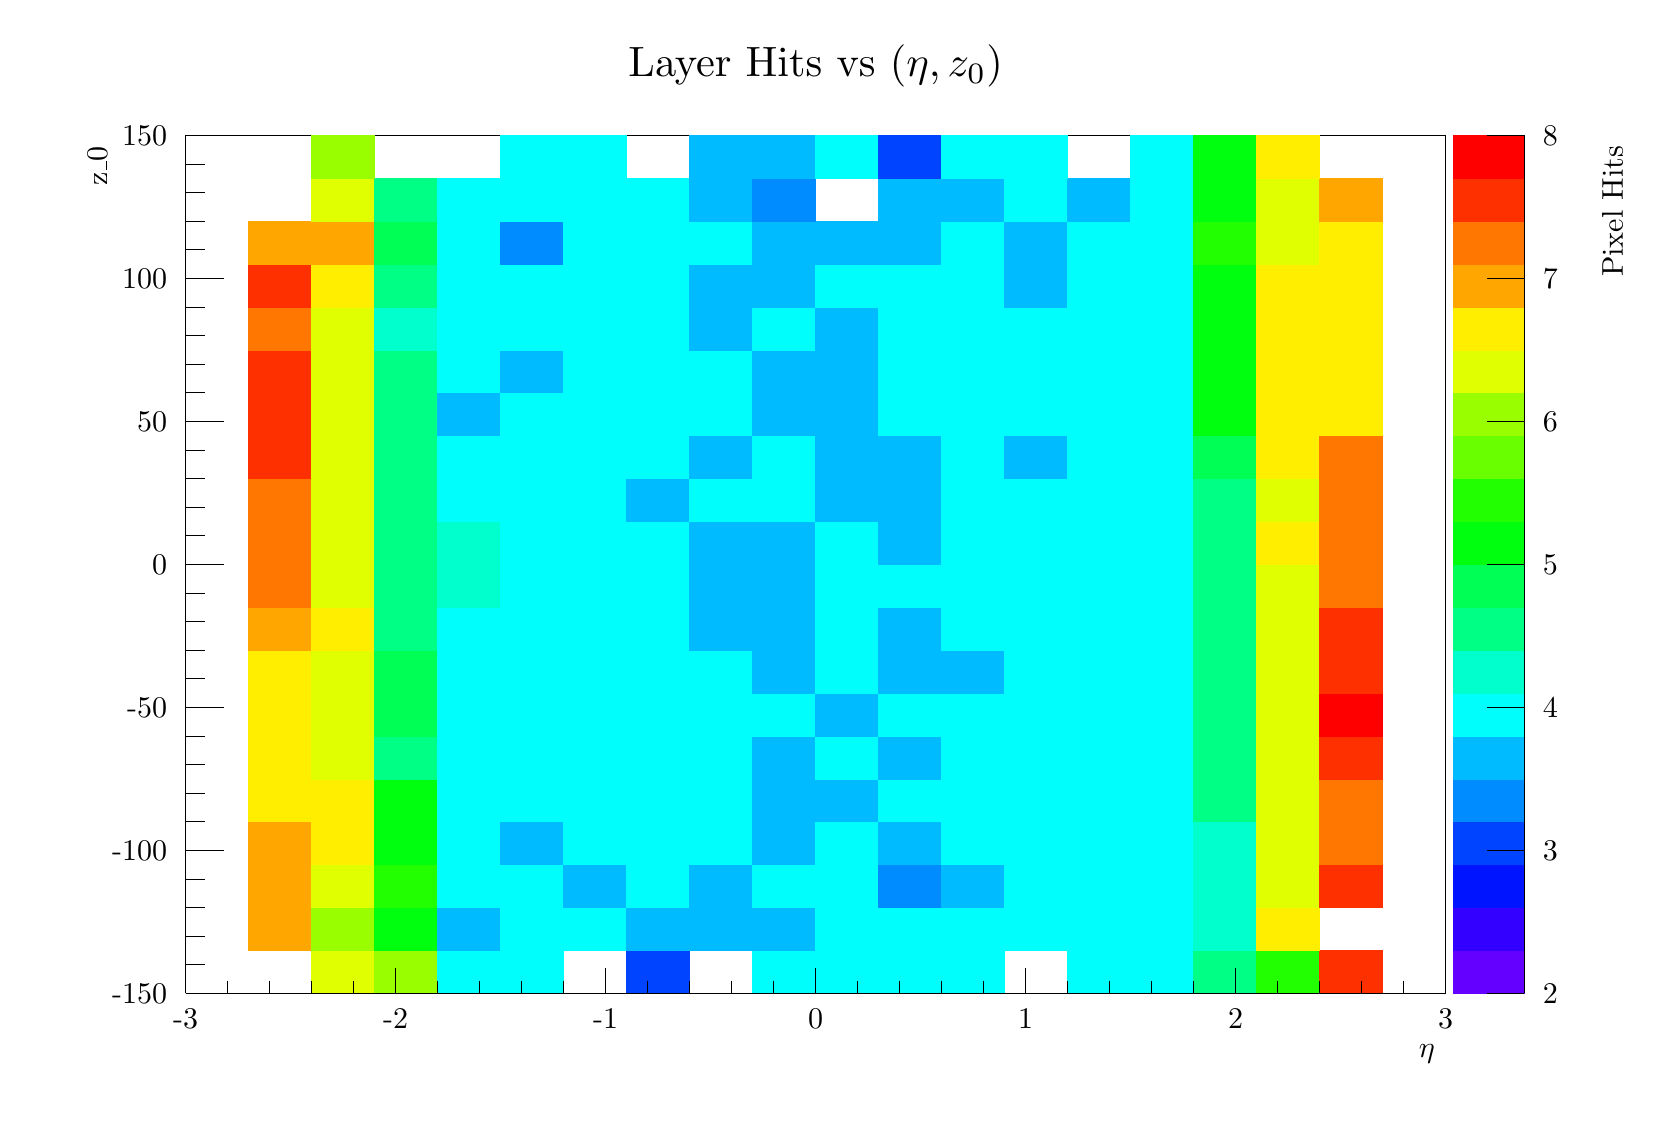
\begin{tikzpicture}
\pgfdeclareplotmark{cross} {
\pgfpathmoveto{\pgfpoint{-0.3\pgfplotmarksize}{\pgfplotmarksize}}
\pgfpathlineto{\pgfpoint{+0.3\pgfplotmarksize}{\pgfplotmarksize}}
\pgfpathlineto{\pgfpoint{+0.3\pgfplotmarksize}{0.3\pgfplotmarksize}}
\pgfpathlineto{\pgfpoint{+1\pgfplotmarksize}{0.3\pgfplotmarksize}}
\pgfpathlineto{\pgfpoint{+1\pgfplotmarksize}{-0.3\pgfplotmarksize}}
\pgfpathlineto{\pgfpoint{+0.3\pgfplotmarksize}{-0.3\pgfplotmarksize}}
\pgfpathlineto{\pgfpoint{+0.3\pgfplotmarksize}{-1.\pgfplotmarksize}}
\pgfpathlineto{\pgfpoint{-0.3\pgfplotmarksize}{-1.\pgfplotmarksize}}
\pgfpathlineto{\pgfpoint{-0.3\pgfplotmarksize}{-0.3\pgfplotmarksize}}
\pgfpathlineto{\pgfpoint{-1.\pgfplotmarksize}{-0.3\pgfplotmarksize}}
\pgfpathlineto{\pgfpoint{-1.\pgfplotmarksize}{0.3\pgfplotmarksize}}
\pgfpathlineto{\pgfpoint{-0.3\pgfplotmarksize}{0.3\pgfplotmarksize}}
\pgfpathclose
\pgfusepathqstroke
}
\pgfdeclareplotmark{cross*} {
\pgfpathmoveto{\pgfpoint{-0.3\pgfplotmarksize}{\pgfplotmarksize}}
\pgfpathlineto{\pgfpoint{+0.3\pgfplotmarksize}{\pgfplotmarksize}}
\pgfpathlineto{\pgfpoint{+0.3\pgfplotmarksize}{0.3\pgfplotmarksize}}
\pgfpathlineto{\pgfpoint{+1\pgfplotmarksize}{0.3\pgfplotmarksize}}
\pgfpathlineto{\pgfpoint{+1\pgfplotmarksize}{-0.3\pgfplotmarksize}}
\pgfpathlineto{\pgfpoint{+0.3\pgfplotmarksize}{-0.3\pgfplotmarksize}}
\pgfpathlineto{\pgfpoint{+0.3\pgfplotmarksize}{-1.\pgfplotmarksize}}
\pgfpathlineto{\pgfpoint{-0.3\pgfplotmarksize}{-1.\pgfplotmarksize}}
\pgfpathlineto{\pgfpoint{-0.3\pgfplotmarksize}{-0.3\pgfplotmarksize}}
\pgfpathlineto{\pgfpoint{-1.\pgfplotmarksize}{-0.3\pgfplotmarksize}}
\pgfpathlineto{\pgfpoint{-1.\pgfplotmarksize}{0.3\pgfplotmarksize}}
\pgfpathlineto{\pgfpoint{-0.3\pgfplotmarksize}{0.3\pgfplotmarksize}}
\pgfpathclose
\pgfusepathqfillstroke
}
\pgfdeclareplotmark{newstar} {
\pgfpathmoveto{\pgfqpoint{0pt}{\pgfplotmarksize}}
\pgfpathlineto{\pgfqpointpolar{44}{0.5\pgfplotmarksize}}
\pgfpathlineto{\pgfqpointpolar{18}{\pgfplotmarksize}}
\pgfpathlineto{\pgfqpointpolar{-20}{0.5\pgfplotmarksize}}
\pgfpathlineto{\pgfqpointpolar{-54}{\pgfplotmarksize}}
\pgfpathlineto{\pgfqpointpolar{-90}{0.5\pgfplotmarksize}}
\pgfpathlineto{\pgfqpointpolar{234}{\pgfplotmarksize}}
\pgfpathlineto{\pgfqpointpolar{198}{0.5\pgfplotmarksize}}
\pgfpathlineto{\pgfqpointpolar{162}{\pgfplotmarksize}}
\pgfpathlineto{\pgfqpointpolar{134}{0.5\pgfplotmarksize}}
\pgfpathclose
\pgfusepathqstroke
}
\pgfdeclareplotmark{newstar*} {
\pgfpathmoveto{\pgfqpoint{0pt}{\pgfplotmarksize}}
\pgfpathlineto{\pgfqpointpolar{44}{0.5\pgfplotmarksize}}
\pgfpathlineto{\pgfqpointpolar{18}{\pgfplotmarksize}}
\pgfpathlineto{\pgfqpointpolar{-20}{0.5\pgfplotmarksize}}
\pgfpathlineto{\pgfqpointpolar{-54}{\pgfplotmarksize}}
\pgfpathlineto{\pgfqpointpolar{-90}{0.5\pgfplotmarksize}}
\pgfpathlineto{\pgfqpointpolar{234}{\pgfplotmarksize}}
\pgfpathlineto{\pgfqpointpolar{198}{0.5\pgfplotmarksize}}
\pgfpathlineto{\pgfqpointpolar{162}{\pgfplotmarksize}}
\pgfpathlineto{\pgfqpointpolar{134}{0.5\pgfplotmarksize}}
\pgfpathclose
\pgfusepathqfillstroke
}
\definecolor{c}{rgb}{1,1,1};
\draw [color=c, fill=c] (0,0) rectangle (20,13.6207);
\draw [color=c, fill=c] (2,1.36207) rectangle (18,12.2586);
\definecolor{c}{rgb}{0,0,0};
\draw [c] (2,1.36207) -- (2,12.2586) -- (18,12.2586) -- (18,1.36207) -- (2,1.36207);
\definecolor{c}{rgb}{1,1,1};
\draw [color=c, fill=c] (2,1.36207) rectangle (18,12.2586);
\definecolor{c}{rgb}{0,0,0};
\draw [c] (2,1.36207) -- (2,12.2586) -- (18,12.2586) -- (18,1.36207) -- (2,1.36207);
\definecolor{c}{rgb}{0.88,1,0};
\draw [color=c, fill=c] (3.6,1.36207) rectangle (4.4,1.9069);
\definecolor{c}{rgb}{0.6,1,0};
\draw [color=c, fill=c] (4.4,1.36207) rectangle (5.2,1.9069);
\definecolor{c}{rgb}{0,1,0.986667};
\draw [color=c, fill=c] (5.2,1.36207) rectangle (6,1.9069);
\draw [color=c, fill=c] (6,1.36207) rectangle (6.8,1.9069);
\definecolor{c}{rgb}{0,0.266667,1};
\draw [color=c, fill=c] (7.6,1.36207) rectangle (8.4,1.9069);
\definecolor{c}{rgb}{0,1,0.986667};
\draw [color=c, fill=c] (9.2,1.36207) rectangle (10,1.9069);
\draw [color=c, fill=c] (10,1.36207) rectangle (10.8,1.9069);
\draw [color=c, fill=c] (10.8,1.36207) rectangle (11.6,1.9069);
\draw [color=c, fill=c] (11.6,1.36207) rectangle (12.4,1.9069);
\draw [color=c, fill=c] (13.2,1.36207) rectangle (14,1.9069);
\draw [color=c, fill=c] (14,1.36207) rectangle (14.8,1.9069);
\definecolor{c}{rgb}{0,1,0.52};
\draw [color=c, fill=c] (14.8,1.36207) rectangle (15.6,1.9069);
\definecolor{c}{rgb}{0.133333,1,0};
\draw [color=c, fill=c] (15.6,1.36207) rectangle (16.4,1.9069);
\definecolor{c}{rgb}{1,0.186667,0};
\draw [color=c, fill=c] (16.4,1.36207) rectangle (17.2,1.9069);
\definecolor{c}{rgb}{1,0.653333,0};
\draw [color=c, fill=c] (2.8,1.9069) rectangle (3.6,2.45172);
\definecolor{c}{rgb}{0.6,1,0};
\draw [color=c, fill=c] (3.6,1.9069) rectangle (4.4,2.45172);
\definecolor{c}{rgb}{0,1,0.0533333};
\draw [color=c, fill=c] (4.4,1.9069) rectangle (5.2,2.45172);
\definecolor{c}{rgb}{0,0.733333,1};
\draw [color=c, fill=c] (5.2,1.9069) rectangle (6,2.45172);
\definecolor{c}{rgb}{0,1,0.986667};
\draw [color=c, fill=c] (6,1.9069) rectangle (6.8,2.45172);
\draw [color=c, fill=c] (6.8,1.9069) rectangle (7.6,2.45172);
\definecolor{c}{rgb}{0,0.733333,1};
\draw [color=c, fill=c] (7.6,1.9069) rectangle (8.4,2.45172);
\draw [color=c, fill=c] (8.4,1.9069) rectangle (9.2,2.45172);
\draw [color=c, fill=c] (9.2,1.9069) rectangle (10,2.45172);
\definecolor{c}{rgb}{0,1,0.986667};
\draw [color=c, fill=c] (10,1.9069) rectangle (10.8,2.45172);
\draw [color=c, fill=c] (10.8,1.9069) rectangle (11.6,2.45172);
\draw [color=c, fill=c] (11.6,1.9069) rectangle (12.4,2.45172);
\draw [color=c, fill=c] (12.4,1.9069) rectangle (13.2,2.45172);
\draw [color=c, fill=c] (13.2,1.9069) rectangle (14,2.45172);
\draw [color=c, fill=c] (14,1.9069) rectangle (14.8,2.45172);
\definecolor{c}{rgb}{0,1,0.8};
\draw [color=c, fill=c] (14.8,1.9069) rectangle (15.6,2.45172);
\definecolor{c}{rgb}{1,0.933333,0};
\draw [color=c, fill=c] (15.6,1.9069) rectangle (16.4,2.45172);
\definecolor{c}{rgb}{1,0.653333,0};
\draw [color=c, fill=c] (2.8,2.45172) rectangle (3.6,2.99655);
\definecolor{c}{rgb}{0.88,1,0};
\draw [color=c, fill=c] (3.6,2.45172) rectangle (4.4,2.99655);
\definecolor{c}{rgb}{0.133333,1,0};
\draw [color=c, fill=c] (4.4,2.45172) rectangle (5.2,2.99655);
\definecolor{c}{rgb}{0,1,0.986667};
\draw [color=c, fill=c] (5.2,2.45172) rectangle (6,2.99655);
\draw [color=c, fill=c] (6,2.45172) rectangle (6.8,2.99655);
\definecolor{c}{rgb}{0,0.733333,1};
\draw [color=c, fill=c] (6.8,2.45172) rectangle (7.6,2.99655);
\definecolor{c}{rgb}{0,1,0.986667};
\draw [color=c, fill=c] (7.6,2.45172) rectangle (8.4,2.99655);
\definecolor{c}{rgb}{0,0.733333,1};
\draw [color=c, fill=c] (8.4,2.45172) rectangle (9.2,2.99655);
\definecolor{c}{rgb}{0,1,0.986667};
\draw [color=c, fill=c] (9.2,2.45172) rectangle (10,2.99655);
\draw [color=c, fill=c] (10,2.45172) rectangle (10.8,2.99655);
\definecolor{c}{rgb}{0,0.546666,1};
\draw [color=c, fill=c] (10.8,2.45172) rectangle (11.6,2.99655);
\definecolor{c}{rgb}{0,0.733333,1};
\draw [color=c, fill=c] (11.6,2.45172) rectangle (12.4,2.99655);
\definecolor{c}{rgb}{0,1,0.986667};
\draw [color=c, fill=c] (12.4,2.45172) rectangle (13.2,2.99655);
\draw [color=c, fill=c] (13.2,2.45172) rectangle (14,2.99655);
\draw [color=c, fill=c] (14,2.45172) rectangle (14.8,2.99655);
\definecolor{c}{rgb}{0,1,0.8};
\draw [color=c, fill=c] (14.8,2.45172) rectangle (15.6,2.99655);
\definecolor{c}{rgb}{0.88,1,0};
\draw [color=c, fill=c] (15.6,2.45172) rectangle (16.4,2.99655);
\definecolor{c}{rgb}{1,0.186667,0};
\draw [color=c, fill=c] (16.4,2.45172) rectangle (17.2,2.99655);
\definecolor{c}{rgb}{1,0.653333,0};
\draw [color=c, fill=c] (2.8,2.99655) rectangle (3.6,3.54138);
\definecolor{c}{rgb}{1,0.933333,0};
\draw [color=c, fill=c] (3.6,2.99655) rectangle (4.4,3.54138);
\definecolor{c}{rgb}{0,1,0.0533333};
\draw [color=c, fill=c] (4.4,2.99655) rectangle (5.2,3.54138);
\definecolor{c}{rgb}{0,1,0.986667};
\draw [color=c, fill=c] (5.2,2.99655) rectangle (6,3.54138);
\definecolor{c}{rgb}{0,0.733333,1};
\draw [color=c, fill=c] (6,2.99655) rectangle (6.8,3.54138);
\definecolor{c}{rgb}{0,1,0.986667};
\draw [color=c, fill=c] (6.8,2.99655) rectangle (7.6,3.54138);
\draw [color=c, fill=c] (7.6,2.99655) rectangle (8.4,3.54138);
\draw [color=c, fill=c] (8.4,2.99655) rectangle (9.2,3.54138);
\definecolor{c}{rgb}{0,0.733333,1};
\draw [color=c, fill=c] (9.2,2.99655) rectangle (10,3.54138);
\definecolor{c}{rgb}{0,1,0.986667};
\draw [color=c, fill=c] (10,2.99655) rectangle (10.8,3.54138);
\definecolor{c}{rgb}{0,0.733333,1};
\draw [color=c, fill=c] (10.8,2.99655) rectangle (11.6,3.54138);
\definecolor{c}{rgb}{0,1,0.986667};
\draw [color=c, fill=c] (11.6,2.99655) rectangle (12.4,3.54138);
\draw [color=c, fill=c] (12.4,2.99655) rectangle (13.2,3.54138);
\draw [color=c, fill=c] (13.2,2.99655) rectangle (14,3.54138);
\draw [color=c, fill=c] (14,2.99655) rectangle (14.8,3.54138);
\definecolor{c}{rgb}{0,1,0.8};
\draw [color=c, fill=c] (14.8,2.99655) rectangle (15.6,3.54138);
\definecolor{c}{rgb}{0.88,1,0};
\draw [color=c, fill=c] (15.6,2.99655) rectangle (16.4,3.54138);
\definecolor{c}{rgb}{1,0.466667,0};
\draw [color=c, fill=c] (16.4,2.99655) rectangle (17.2,3.54138);
\definecolor{c}{rgb}{1,0.933333,0};
\draw [color=c, fill=c] (2.8,3.54138) rectangle (3.6,4.08621);
\draw [color=c, fill=c] (3.6,3.54138) rectangle (4.4,4.08621);
\definecolor{c}{rgb}{0,1,0.0533333};
\draw [color=c, fill=c] (4.4,3.54138) rectangle (5.2,4.08621);
\definecolor{c}{rgb}{0,1,0.986667};
\draw [color=c, fill=c] (5.2,3.54138) rectangle (6,4.08621);
\draw [color=c, fill=c] (6,3.54138) rectangle (6.8,4.08621);
\draw [color=c, fill=c] (6.8,3.54138) rectangle (7.6,4.08621);
\draw [color=c, fill=c] (7.6,3.54138) rectangle (8.4,4.08621);
\draw [color=c, fill=c] (8.4,3.54138) rectangle (9.2,4.08621);
\definecolor{c}{rgb}{0,0.733333,1};
\draw [color=c, fill=c] (9.2,3.54138) rectangle (10,4.08621);
\draw [color=c, fill=c] (10,3.54138) rectangle (10.8,4.08621);
\definecolor{c}{rgb}{0,1,0.986667};
\draw [color=c, fill=c] (10.8,3.54138) rectangle (11.6,4.08621);
\draw [color=c, fill=c] (11.6,3.54138) rectangle (12.4,4.08621);
\draw [color=c, fill=c] (12.4,3.54138) rectangle (13.2,4.08621);
\draw [color=c, fill=c] (13.2,3.54138) rectangle (14,4.08621);
\draw [color=c, fill=c] (14,3.54138) rectangle (14.8,4.08621);
\definecolor{c}{rgb}{0,1,0.52};
\draw [color=c, fill=c] (14.8,3.54138) rectangle (15.6,4.08621);
\definecolor{c}{rgb}{0.88,1,0};
\draw [color=c, fill=c] (15.6,3.54138) rectangle (16.4,4.08621);
\definecolor{c}{rgb}{1,0.466667,0};
\draw [color=c, fill=c] (16.4,3.54138) rectangle (17.2,4.08621);
\definecolor{c}{rgb}{1,0.933333,0};
\draw [color=c, fill=c] (2.8,4.08621) rectangle (3.6,4.63103);
\definecolor{c}{rgb}{0.88,1,0};
\draw [color=c, fill=c] (3.6,4.08621) rectangle (4.4,4.63103);
\definecolor{c}{rgb}{0,1,0.52};
\draw [color=c, fill=c] (4.4,4.08621) rectangle (5.2,4.63103);
\definecolor{c}{rgb}{0,1,0.986667};
\draw [color=c, fill=c] (5.2,4.08621) rectangle (6,4.63103);
\draw [color=c, fill=c] (6,4.08621) rectangle (6.8,4.63103);
\draw [color=c, fill=c] (6.8,4.08621) rectangle (7.6,4.63103);
\draw [color=c, fill=c] (7.6,4.08621) rectangle (8.4,4.63103);
\draw [color=c, fill=c] (8.4,4.08621) rectangle (9.2,4.63103);
\definecolor{c}{rgb}{0,0.733333,1};
\draw [color=c, fill=c] (9.2,4.08621) rectangle (10,4.63103);
\definecolor{c}{rgb}{0,1,0.986667};
\draw [color=c, fill=c] (10,4.08621) rectangle (10.8,4.63103);
\definecolor{c}{rgb}{0,0.733333,1};
\draw [color=c, fill=c] (10.8,4.08621) rectangle (11.6,4.63103);
\definecolor{c}{rgb}{0,1,0.986667};
\draw [color=c, fill=c] (11.6,4.08621) rectangle (12.4,4.63103);
\draw [color=c, fill=c] (12.4,4.08621) rectangle (13.2,4.63103);
\draw [color=c, fill=c] (13.2,4.08621) rectangle (14,4.63103);
\draw [color=c, fill=c] (14,4.08621) rectangle (14.8,4.63103);
\definecolor{c}{rgb}{0,1,0.52};
\draw [color=c, fill=c] (14.8,4.08621) rectangle (15.6,4.63103);
\definecolor{c}{rgb}{0.88,1,0};
\draw [color=c, fill=c] (15.6,4.08621) rectangle (16.4,4.63103);
\definecolor{c}{rgb}{1,0.186667,0};
\draw [color=c, fill=c] (16.4,4.08621) rectangle (17.2,4.63103);
\definecolor{c}{rgb}{1,0.933333,0};
\draw [color=c, fill=c] (2.8,4.63103) rectangle (3.6,5.17586);
\definecolor{c}{rgb}{0.88,1,0};
\draw [color=c, fill=c] (3.6,4.63103) rectangle (4.4,5.17586);
\definecolor{c}{rgb}{0,1,0.333333};
\draw [color=c, fill=c] (4.4,4.63103) rectangle (5.2,5.17586);
\definecolor{c}{rgb}{0,1,0.986667};
\draw [color=c, fill=c] (5.2,4.63103) rectangle (6,5.17586);
\draw [color=c, fill=c] (6,4.63103) rectangle (6.8,5.17586);
\draw [color=c, fill=c] (6.8,4.63103) rectangle (7.6,5.17586);
\draw [color=c, fill=c] (7.6,4.63103) rectangle (8.4,5.17586);
\draw [color=c, fill=c] (8.4,4.63103) rectangle (9.2,5.17586);
\draw [color=c, fill=c] (9.2,4.63103) rectangle (10,5.17586);
\definecolor{c}{rgb}{0,0.733333,1};
\draw [color=c, fill=c] (10,4.63103) rectangle (10.8,5.17586);
\definecolor{c}{rgb}{0,1,0.986667};
\draw [color=c, fill=c] (10.8,4.63103) rectangle (11.6,5.17586);
\draw [color=c, fill=c] (11.6,4.63103) rectangle (12.4,5.17586);
\draw [color=c, fill=c] (12.4,4.63103) rectangle (13.2,5.17586);
\draw [color=c, fill=c] (13.2,4.63103) rectangle (14,5.17586);
\draw [color=c, fill=c] (14,4.63103) rectangle (14.8,5.17586);
\definecolor{c}{rgb}{0,1,0.52};
\draw [color=c, fill=c] (14.8,4.63103) rectangle (15.6,5.17586);
\definecolor{c}{rgb}{0.88,1,0};
\draw [color=c, fill=c] (15.6,4.63103) rectangle (16.4,5.17586);
\definecolor{c}{rgb}{1,0,0};
\draw [color=c, fill=c] (16.4,4.63103) rectangle (17.2,5.17586);
\definecolor{c}{rgb}{1,0.933333,0};
\draw [color=c, fill=c] (2.8,5.17586) rectangle (3.6,5.72069);
\definecolor{c}{rgb}{0.88,1,0};
\draw [color=c, fill=c] (3.6,5.17586) rectangle (4.4,5.72069);
\definecolor{c}{rgb}{0,1,0.333333};
\draw [color=c, fill=c] (4.4,5.17586) rectangle (5.2,5.72069);
\definecolor{c}{rgb}{0,1,0.986667};
\draw [color=c, fill=c] (5.2,5.17586) rectangle (6,5.72069);
\draw [color=c, fill=c] (6,5.17586) rectangle (6.8,5.72069);
\draw [color=c, fill=c] (6.8,5.17586) rectangle (7.6,5.72069);
\draw [color=c, fill=c] (7.6,5.17586) rectangle (8.4,5.72069);
\draw [color=c, fill=c] (8.4,5.17586) rectangle (9.2,5.72069);
\definecolor{c}{rgb}{0,0.733333,1};
\draw [color=c, fill=c] (9.2,5.17586) rectangle (10,5.72069);
\definecolor{c}{rgb}{0,1,0.986667};
\draw [color=c, fill=c] (10,5.17586) rectangle (10.8,5.72069);
\definecolor{c}{rgb}{0,0.733333,1};
\draw [color=c, fill=c] (10.8,5.17586) rectangle (11.6,5.72069);
\draw [color=c, fill=c] (11.6,5.17586) rectangle (12.4,5.72069);
\definecolor{c}{rgb}{0,1,0.986667};
\draw [color=c, fill=c] (12.4,5.17586) rectangle (13.2,5.72069);
\draw [color=c, fill=c] (13.2,5.17586) rectangle (14,5.72069);
\draw [color=c, fill=c] (14,5.17586) rectangle (14.8,5.72069);
\definecolor{c}{rgb}{0,1,0.52};
\draw [color=c, fill=c] (14.8,5.17586) rectangle (15.6,5.72069);
\definecolor{c}{rgb}{0.88,1,0};
\draw [color=c, fill=c] (15.6,5.17586) rectangle (16.4,5.72069);
\definecolor{c}{rgb}{1,0.186667,0};
\draw [color=c, fill=c] (16.4,5.17586) rectangle (17.2,5.72069);
\definecolor{c}{rgb}{1,0.653333,0};
\draw [color=c, fill=c] (2.8,5.72069) rectangle (3.6,6.26552);
\definecolor{c}{rgb}{1,0.933333,0};
\draw [color=c, fill=c] (3.6,5.72069) rectangle (4.4,6.26552);
\definecolor{c}{rgb}{0,1,0.52};
\draw [color=c, fill=c] (4.4,5.72069) rectangle (5.2,6.26552);
\definecolor{c}{rgb}{0,1,0.986667};
\draw [color=c, fill=c] (5.2,5.72069) rectangle (6,6.26552);
\draw [color=c, fill=c] (6,5.72069) rectangle (6.8,6.26552);
\draw [color=c, fill=c] (6.8,5.72069) rectangle (7.6,6.26552);
\draw [color=c, fill=c] (7.6,5.72069) rectangle (8.4,6.26552);
\definecolor{c}{rgb}{0,0.733333,1};
\draw [color=c, fill=c] (8.4,5.72069) rectangle (9.2,6.26552);
\draw [color=c, fill=c] (9.2,5.72069) rectangle (10,6.26552);
\definecolor{c}{rgb}{0,1,0.986667};
\draw [color=c, fill=c] (10,5.72069) rectangle (10.8,6.26552);
\definecolor{c}{rgb}{0,0.733333,1};
\draw [color=c, fill=c] (10.8,5.72069) rectangle (11.6,6.26552);
\definecolor{c}{rgb}{0,1,0.986667};
\draw [color=c, fill=c] (11.6,5.72069) rectangle (12.4,6.26552);
\draw [color=c, fill=c] (12.4,5.72069) rectangle (13.2,6.26552);
\draw [color=c, fill=c] (13.2,5.72069) rectangle (14,6.26552);
\draw [color=c, fill=c] (14,5.72069) rectangle (14.8,6.26552);
\definecolor{c}{rgb}{0,1,0.52};
\draw [color=c, fill=c] (14.8,5.72069) rectangle (15.6,6.26552);
\definecolor{c}{rgb}{0.88,1,0};
\draw [color=c, fill=c] (15.6,5.72069) rectangle (16.4,6.26552);
\definecolor{c}{rgb}{1,0.186667,0};
\draw [color=c, fill=c] (16.4,5.72069) rectangle (17.2,6.26552);
\definecolor{c}{rgb}{1,0.466667,0};
\draw [color=c, fill=c] (2.8,6.26552) rectangle (3.6,6.81034);
\definecolor{c}{rgb}{0.88,1,0};
\draw [color=c, fill=c] (3.6,6.26552) rectangle (4.4,6.81034);
\definecolor{c}{rgb}{0,1,0.52};
\draw [color=c, fill=c] (4.4,6.26552) rectangle (5.2,6.81034);
\definecolor{c}{rgb}{0,1,0.8};
\draw [color=c, fill=c] (5.2,6.26552) rectangle (6,6.81034);
\definecolor{c}{rgb}{0,1,0.986667};
\draw [color=c, fill=c] (6,6.26552) rectangle (6.8,6.81034);
\draw [color=c, fill=c] (6.8,6.26552) rectangle (7.6,6.81034);
\draw [color=c, fill=c] (7.6,6.26552) rectangle (8.4,6.81034);
\definecolor{c}{rgb}{0,0.733333,1};
\draw [color=c, fill=c] (8.4,6.26552) rectangle (9.2,6.81034);
\draw [color=c, fill=c] (9.2,6.26552) rectangle (10,6.81034);
\definecolor{c}{rgb}{0,1,0.986667};
\draw [color=c, fill=c] (10,6.26552) rectangle (10.8,6.81034);
\draw [color=c, fill=c] (10.8,6.26552) rectangle (11.6,6.81034);
\draw [color=c, fill=c] (11.6,6.26552) rectangle (12.4,6.81034);
\draw [color=c, fill=c] (12.4,6.26552) rectangle (13.2,6.81034);
\draw [color=c, fill=c] (13.2,6.26552) rectangle (14,6.81034);
\draw [color=c, fill=c] (14,6.26552) rectangle (14.8,6.81034);
\definecolor{c}{rgb}{0,1,0.52};
\draw [color=c, fill=c] (14.8,6.26552) rectangle (15.6,6.81034);
\definecolor{c}{rgb}{0.88,1,0};
\draw [color=c, fill=c] (15.6,6.26552) rectangle (16.4,6.81034);
\definecolor{c}{rgb}{1,0.466667,0};
\draw [color=c, fill=c] (16.4,6.26552) rectangle (17.2,6.81034);
\draw [color=c, fill=c] (2.8,6.81034) rectangle (3.6,7.35517);
\definecolor{c}{rgb}{0.88,1,0};
\draw [color=c, fill=c] (3.6,6.81034) rectangle (4.4,7.35517);
\definecolor{c}{rgb}{0,1,0.52};
\draw [color=c, fill=c] (4.4,6.81034) rectangle (5.2,7.35517);
\definecolor{c}{rgb}{0,1,0.8};
\draw [color=c, fill=c] (5.2,6.81034) rectangle (6,7.35517);
\definecolor{c}{rgb}{0,1,0.986667};
\draw [color=c, fill=c] (6,6.81034) rectangle (6.8,7.35517);
\draw [color=c, fill=c] (6.8,6.81034) rectangle (7.6,7.35517);
\draw [color=c, fill=c] (7.6,6.81034) rectangle (8.4,7.35517);
\definecolor{c}{rgb}{0,0.733333,1};
\draw [color=c, fill=c] (8.4,6.81034) rectangle (9.2,7.35517);
\draw [color=c, fill=c] (9.2,6.81034) rectangle (10,7.35517);
\definecolor{c}{rgb}{0,1,0.986667};
\draw [color=c, fill=c] (10,6.81034) rectangle (10.8,7.35517);
\definecolor{c}{rgb}{0,0.733333,1};
\draw [color=c, fill=c] (10.8,6.81034) rectangle (11.6,7.35517);
\definecolor{c}{rgb}{0,1,0.986667};
\draw [color=c, fill=c] (11.6,6.81034) rectangle (12.4,7.35517);
\draw [color=c, fill=c] (12.4,6.81034) rectangle (13.2,7.35517);
\draw [color=c, fill=c] (13.2,6.81034) rectangle (14,7.35517);
\draw [color=c, fill=c] (14,6.81034) rectangle (14.8,7.35517);
\definecolor{c}{rgb}{0,1,0.52};
\draw [color=c, fill=c] (14.8,6.81034) rectangle (15.6,7.35517);
\definecolor{c}{rgb}{1,0.933333,0};
\draw [color=c, fill=c] (15.6,6.81034) rectangle (16.4,7.35517);
\definecolor{c}{rgb}{1,0.466667,0};
\draw [color=c, fill=c] (16.4,6.81034) rectangle (17.2,7.35517);
\draw [color=c, fill=c] (2.8,7.35517) rectangle (3.6,7.9);
\definecolor{c}{rgb}{0.88,1,0};
\draw [color=c, fill=c] (3.6,7.35517) rectangle (4.4,7.9);
\definecolor{c}{rgb}{0,1,0.52};
\draw [color=c, fill=c] (4.4,7.35517) rectangle (5.2,7.9);
\definecolor{c}{rgb}{0,1,0.986667};
\draw [color=c, fill=c] (5.2,7.35517) rectangle (6,7.9);
\draw [color=c, fill=c] (6,7.35517) rectangle (6.8,7.9);
\draw [color=c, fill=c] (6.8,7.35517) rectangle (7.6,7.9);
\definecolor{c}{rgb}{0,0.733333,1};
\draw [color=c, fill=c] (7.6,7.35517) rectangle (8.4,7.9);
\definecolor{c}{rgb}{0,1,0.986667};
\draw [color=c, fill=c] (8.4,7.35517) rectangle (9.2,7.9);
\draw [color=c, fill=c] (9.2,7.35517) rectangle (10,7.9);
\definecolor{c}{rgb}{0,0.733333,1};
\draw [color=c, fill=c] (10,7.35517) rectangle (10.8,7.9);
\draw [color=c, fill=c] (10.8,7.35517) rectangle (11.6,7.9);
\definecolor{c}{rgb}{0,1,0.986667};
\draw [color=c, fill=c] (11.6,7.35517) rectangle (12.4,7.9);
\draw [color=c, fill=c] (12.4,7.35517) rectangle (13.2,7.9);
\draw [color=c, fill=c] (13.2,7.35517) rectangle (14,7.9);
\draw [color=c, fill=c] (14,7.35517) rectangle (14.8,7.9);
\definecolor{c}{rgb}{0,1,0.52};
\draw [color=c, fill=c] (14.8,7.35517) rectangle (15.6,7.9);
\definecolor{c}{rgb}{0.88,1,0};
\draw [color=c, fill=c] (15.6,7.35517) rectangle (16.4,7.9);
\definecolor{c}{rgb}{1,0.466667,0};
\draw [color=c, fill=c] (16.4,7.35517) rectangle (17.2,7.9);
\definecolor{c}{rgb}{1,0.186667,0};
\draw [color=c, fill=c] (2.8,7.9) rectangle (3.6,8.44483);
\definecolor{c}{rgb}{0.88,1,0};
\draw [color=c, fill=c] (3.6,7.9) rectangle (4.4,8.44483);
\definecolor{c}{rgb}{0,1,0.52};
\draw [color=c, fill=c] (4.4,7.9) rectangle (5.2,8.44483);
\definecolor{c}{rgb}{0,1,0.986667};
\draw [color=c, fill=c] (5.2,7.9) rectangle (6,8.44483);
\draw [color=c, fill=c] (6,7.9) rectangle (6.8,8.44483);
\draw [color=c, fill=c] (6.8,7.9) rectangle (7.6,8.44483);
\draw [color=c, fill=c] (7.6,7.9) rectangle (8.4,8.44483);
\definecolor{c}{rgb}{0,0.733333,1};
\draw [color=c, fill=c] (8.4,7.9) rectangle (9.2,8.44483);
\definecolor{c}{rgb}{0,1,0.986667};
\draw [color=c, fill=c] (9.2,7.9) rectangle (10,8.44483);
\definecolor{c}{rgb}{0,0.733333,1};
\draw [color=c, fill=c] (10,7.9) rectangle (10.8,8.44483);
\draw [color=c, fill=c] (10.8,7.9) rectangle (11.6,8.44483);
\definecolor{c}{rgb}{0,1,0.986667};
\draw [color=c, fill=c] (11.6,7.9) rectangle (12.4,8.44483);
\definecolor{c}{rgb}{0,0.733333,1};
\draw [color=c, fill=c] (12.4,7.9) rectangle (13.2,8.44483);
\definecolor{c}{rgb}{0,1,0.986667};
\draw [color=c, fill=c] (13.2,7.9) rectangle (14,8.44483);
\draw [color=c, fill=c] (14,7.9) rectangle (14.8,8.44483);
\definecolor{c}{rgb}{0,1,0.333333};
\draw [color=c, fill=c] (14.8,7.9) rectangle (15.6,8.44483);
\definecolor{c}{rgb}{1,0.933333,0};
\draw [color=c, fill=c] (15.6,7.9) rectangle (16.4,8.44483);
\definecolor{c}{rgb}{1,0.466667,0};
\draw [color=c, fill=c] (16.4,7.9) rectangle (17.2,8.44483);
\definecolor{c}{rgb}{1,0.186667,0};
\draw [color=c, fill=c] (2.8,8.44483) rectangle (3.6,8.98965);
\definecolor{c}{rgb}{0.88,1,0};
\draw [color=c, fill=c] (3.6,8.44483) rectangle (4.4,8.98965);
\definecolor{c}{rgb}{0,1,0.52};
\draw [color=c, fill=c] (4.4,8.44483) rectangle (5.2,8.98965);
\definecolor{c}{rgb}{0,0.733333,1};
\draw [color=c, fill=c] (5.2,8.44483) rectangle (6,8.98965);
\definecolor{c}{rgb}{0,1,0.986667};
\draw [color=c, fill=c] (6,8.44483) rectangle (6.8,8.98965);
\draw [color=c, fill=c] (6.8,8.44483) rectangle (7.6,8.98965);
\draw [color=c, fill=c] (7.6,8.44483) rectangle (8.4,8.98965);
\draw [color=c, fill=c] (8.4,8.44483) rectangle (9.2,8.98965);
\definecolor{c}{rgb}{0,0.733333,1};
\draw [color=c, fill=c] (9.2,8.44483) rectangle (10,8.98965);
\draw [color=c, fill=c] (10,8.44483) rectangle (10.8,8.98965);
\definecolor{c}{rgb}{0,1,0.986667};
\draw [color=c, fill=c] (10.8,8.44483) rectangle (11.6,8.98965);
\draw [color=c, fill=c] (11.6,8.44483) rectangle (12.4,8.98965);
\draw [color=c, fill=c] (12.4,8.44483) rectangle (13.2,8.98965);
\draw [color=c, fill=c] (13.2,8.44483) rectangle (14,8.98965);
\draw [color=c, fill=c] (14,8.44483) rectangle (14.8,8.98965);
\definecolor{c}{rgb}{0,1,0.0533333};
\draw [color=c, fill=c] (14.8,8.44483) rectangle (15.6,8.98965);
\definecolor{c}{rgb}{1,0.933333,0};
\draw [color=c, fill=c] (15.6,8.44483) rectangle (16.4,8.98965);
\draw [color=c, fill=c] (16.4,8.44483) rectangle (17.2,8.98965);
\definecolor{c}{rgb}{1,0.186667,0};
\draw [color=c, fill=c] (2.8,8.98965) rectangle (3.6,9.53448);
\definecolor{c}{rgb}{0.88,1,0};
\draw [color=c, fill=c] (3.6,8.98965) rectangle (4.4,9.53448);
\definecolor{c}{rgb}{0,1,0.52};
\draw [color=c, fill=c] (4.4,8.98965) rectangle (5.2,9.53448);
\definecolor{c}{rgb}{0,1,0.986667};
\draw [color=c, fill=c] (5.2,8.98965) rectangle (6,9.53448);
\definecolor{c}{rgb}{0,0.733333,1};
\draw [color=c, fill=c] (6,8.98965) rectangle (6.8,9.53448);
\definecolor{c}{rgb}{0,1,0.986667};
\draw [color=c, fill=c] (6.8,8.98965) rectangle (7.6,9.53448);
\draw [color=c, fill=c] (7.6,8.98965) rectangle (8.4,9.53448);
\draw [color=c, fill=c] (8.4,8.98965) rectangle (9.2,9.53448);
\definecolor{c}{rgb}{0,0.733333,1};
\draw [color=c, fill=c] (9.2,8.98965) rectangle (10,9.53448);
\draw [color=c, fill=c] (10,8.98965) rectangle (10.8,9.53448);
\definecolor{c}{rgb}{0,1,0.986667};
\draw [color=c, fill=c] (10.8,8.98965) rectangle (11.6,9.53448);
\draw [color=c, fill=c] (11.6,8.98965) rectangle (12.4,9.53448);
\draw [color=c, fill=c] (12.4,8.98965) rectangle (13.2,9.53448);
\draw [color=c, fill=c] (13.2,8.98965) rectangle (14,9.53448);
\draw [color=c, fill=c] (14,8.98965) rectangle (14.8,9.53448);
\definecolor{c}{rgb}{0,1,0.0533333};
\draw [color=c, fill=c] (14.8,8.98965) rectangle (15.6,9.53448);
\definecolor{c}{rgb}{1,0.933333,0};
\draw [color=c, fill=c] (15.6,8.98965) rectangle (16.4,9.53448);
\draw [color=c, fill=c] (16.4,8.98965) rectangle (17.2,9.53448);
\definecolor{c}{rgb}{1,0.466667,0};
\draw [color=c, fill=c] (2.8,9.53448) rectangle (3.6,10.0793);
\definecolor{c}{rgb}{0.88,1,0};
\draw [color=c, fill=c] (3.6,9.53448) rectangle (4.4,10.0793);
\definecolor{c}{rgb}{0,1,0.8};
\draw [color=c, fill=c] (4.4,9.53448) rectangle (5.2,10.0793);
\definecolor{c}{rgb}{0,1,0.986667};
\draw [color=c, fill=c] (5.2,9.53448) rectangle (6,10.0793);
\draw [color=c, fill=c] (6,9.53448) rectangle (6.8,10.0793);
\draw [color=c, fill=c] (6.8,9.53448) rectangle (7.6,10.0793);
\draw [color=c, fill=c] (7.6,9.53448) rectangle (8.4,10.0793);
\definecolor{c}{rgb}{0,0.733333,1};
\draw [color=c, fill=c] (8.4,9.53448) rectangle (9.2,10.0793);
\definecolor{c}{rgb}{0,1,0.986667};
\draw [color=c, fill=c] (9.2,9.53448) rectangle (10,10.0793);
\definecolor{c}{rgb}{0,0.733333,1};
\draw [color=c, fill=c] (10,9.53448) rectangle (10.8,10.0793);
\definecolor{c}{rgb}{0,1,0.986667};
\draw [color=c, fill=c] (10.8,9.53448) rectangle (11.6,10.0793);
\draw [color=c, fill=c] (11.6,9.53448) rectangle (12.4,10.0793);
\draw [color=c, fill=c] (12.4,9.53448) rectangle (13.2,10.0793);
\draw [color=c, fill=c] (13.2,9.53448) rectangle (14,10.0793);
\draw [color=c, fill=c] (14,9.53448) rectangle (14.8,10.0793);
\definecolor{c}{rgb}{0,1,0.0533333};
\draw [color=c, fill=c] (14.8,9.53448) rectangle (15.6,10.0793);
\definecolor{c}{rgb}{1,0.933333,0};
\draw [color=c, fill=c] (15.6,9.53448) rectangle (16.4,10.0793);
\draw [color=c, fill=c] (16.4,9.53448) rectangle (17.2,10.0793);
\definecolor{c}{rgb}{1,0.186667,0};
\draw [color=c, fill=c] (2.8,10.0793) rectangle (3.6,10.6241);
\definecolor{c}{rgb}{1,0.933333,0};
\draw [color=c, fill=c] (3.6,10.0793) rectangle (4.4,10.6241);
\definecolor{c}{rgb}{0,1,0.52};
\draw [color=c, fill=c] (4.4,10.0793) rectangle (5.2,10.6241);
\definecolor{c}{rgb}{0,1,0.986667};
\draw [color=c, fill=c] (5.2,10.0793) rectangle (6,10.6241);
\draw [color=c, fill=c] (6,10.0793) rectangle (6.8,10.6241);
\draw [color=c, fill=c] (6.8,10.0793) rectangle (7.6,10.6241);
\draw [color=c, fill=c] (7.6,10.0793) rectangle (8.4,10.6241);
\definecolor{c}{rgb}{0,0.733333,1};
\draw [color=c, fill=c] (8.4,10.0793) rectangle (9.2,10.6241);
\draw [color=c, fill=c] (9.2,10.0793) rectangle (10,10.6241);
\definecolor{c}{rgb}{0,1,0.986667};
\draw [color=c, fill=c] (10,10.0793) rectangle (10.8,10.6241);
\draw [color=c, fill=c] (10.8,10.0793) rectangle (11.6,10.6241);
\draw [color=c, fill=c] (11.6,10.0793) rectangle (12.4,10.6241);
\definecolor{c}{rgb}{0,0.733333,1};
\draw [color=c, fill=c] (12.4,10.0793) rectangle (13.2,10.6241);
\definecolor{c}{rgb}{0,1,0.986667};
\draw [color=c, fill=c] (13.2,10.0793) rectangle (14,10.6241);
\draw [color=c, fill=c] (14,10.0793) rectangle (14.8,10.6241);
\definecolor{c}{rgb}{0,1,0.0533333};
\draw [color=c, fill=c] (14.8,10.0793) rectangle (15.6,10.6241);
\definecolor{c}{rgb}{1,0.933333,0};
\draw [color=c, fill=c] (15.6,10.0793) rectangle (16.4,10.6241);
\draw [color=c, fill=c] (16.4,10.0793) rectangle (17.2,10.6241);
\definecolor{c}{rgb}{1,0.653333,0};
\draw [color=c, fill=c] (2.8,10.6241) rectangle (3.6,11.169);
\draw [color=c, fill=c] (3.6,10.6241) rectangle (4.4,11.169);
\definecolor{c}{rgb}{0,1,0.333333};
\draw [color=c, fill=c] (4.4,10.6241) rectangle (5.2,11.169);
\definecolor{c}{rgb}{0,1,0.986667};
\draw [color=c, fill=c] (5.2,10.6241) rectangle (6,11.169);
\definecolor{c}{rgb}{0,0.546666,1};
\draw [color=c, fill=c] (6,10.6241) rectangle (6.8,11.169);
\definecolor{c}{rgb}{0,1,0.986667};
\draw [color=c, fill=c] (6.8,10.6241) rectangle (7.6,11.169);
\draw [color=c, fill=c] (7.6,10.6241) rectangle (8.4,11.169);
\draw [color=c, fill=c] (8.4,10.6241) rectangle (9.2,11.169);
\definecolor{c}{rgb}{0,0.733333,1};
\draw [color=c, fill=c] (9.2,10.6241) rectangle (10,11.169);
\draw [color=c, fill=c] (10,10.6241) rectangle (10.8,11.169);
\draw [color=c, fill=c] (10.8,10.6241) rectangle (11.6,11.169);
\definecolor{c}{rgb}{0,1,0.986667};
\draw [color=c, fill=c] (11.6,10.6241) rectangle (12.4,11.169);
\definecolor{c}{rgb}{0,0.733333,1};
\draw [color=c, fill=c] (12.4,10.6241) rectangle (13.2,11.169);
\definecolor{c}{rgb}{0,1,0.986667};
\draw [color=c, fill=c] (13.2,10.6241) rectangle (14,11.169);
\draw [color=c, fill=c] (14,10.6241) rectangle (14.8,11.169);
\definecolor{c}{rgb}{0.133333,1,0};
\draw [color=c, fill=c] (14.8,10.6241) rectangle (15.6,11.169);
\definecolor{c}{rgb}{0.88,1,0};
\draw [color=c, fill=c] (15.6,10.6241) rectangle (16.4,11.169);
\definecolor{c}{rgb}{1,0.933333,0};
\draw [color=c, fill=c] (16.4,10.6241) rectangle (17.2,11.169);
\definecolor{c}{rgb}{0.88,1,0};
\draw [color=c, fill=c] (3.6,11.169) rectangle (4.4,11.7138);
\definecolor{c}{rgb}{0,1,0.52};
\draw [color=c, fill=c] (4.4,11.169) rectangle (5.2,11.7138);
\definecolor{c}{rgb}{0,1,0.986667};
\draw [color=c, fill=c] (5.2,11.169) rectangle (6,11.7138);
\draw [color=c, fill=c] (6,11.169) rectangle (6.8,11.7138);
\draw [color=c, fill=c] (6.8,11.169) rectangle (7.6,11.7138);
\draw [color=c, fill=c] (7.6,11.169) rectangle (8.4,11.7138);
\definecolor{c}{rgb}{0,0.733333,1};
\draw [color=c, fill=c] (8.4,11.169) rectangle (9.2,11.7138);
\definecolor{c}{rgb}{0,0.546666,1};
\draw [color=c, fill=c] (9.2,11.169) rectangle (10,11.7138);
\definecolor{c}{rgb}{0,0.733333,1};
\draw [color=c, fill=c] (10.8,11.169) rectangle (11.6,11.7138);
\draw [color=c, fill=c] (11.6,11.169) rectangle (12.4,11.7138);
\definecolor{c}{rgb}{0,1,0.986667};
\draw [color=c, fill=c] (12.4,11.169) rectangle (13.2,11.7138);
\definecolor{c}{rgb}{0,0.733333,1};
\draw [color=c, fill=c] (13.2,11.169) rectangle (14,11.7138);
\definecolor{c}{rgb}{0,1,0.986667};
\draw [color=c, fill=c] (14,11.169) rectangle (14.8,11.7138);
\definecolor{c}{rgb}{0,1,0.0533333};
\draw [color=c, fill=c] (14.8,11.169) rectangle (15.6,11.7138);
\definecolor{c}{rgb}{0.88,1,0};
\draw [color=c, fill=c] (15.6,11.169) rectangle (16.4,11.7138);
\definecolor{c}{rgb}{1,0.653333,0};
\draw [color=c, fill=c] (16.4,11.169) rectangle (17.2,11.7138);
\definecolor{c}{rgb}{0.6,1,0};
\draw [color=c, fill=c] (3.6,11.7138) rectangle (4.4,12.2586);
\definecolor{c}{rgb}{0,1,0.986667};
\draw [color=c, fill=c] (6,11.7138) rectangle (6.8,12.2586);
\draw [color=c, fill=c] (6.8,11.7138) rectangle (7.6,12.2586);
\definecolor{c}{rgb}{0,0.733333,1};
\draw [color=c, fill=c] (8.4,11.7138) rectangle (9.2,12.2586);
\draw [color=c, fill=c] (9.2,11.7138) rectangle (10,12.2586);
\definecolor{c}{rgb}{0,1,0.986667};
\draw [color=c, fill=c] (10,11.7138) rectangle (10.8,12.2586);
\definecolor{c}{rgb}{0,0.266667,1};
\draw [color=c, fill=c] (10.8,11.7138) rectangle (11.6,12.2586);
\definecolor{c}{rgb}{0,1,0.986667};
\draw [color=c, fill=c] (11.6,11.7138) rectangle (12.4,12.2586);
\draw [color=c, fill=c] (12.4,11.7138) rectangle (13.2,12.2586);
\draw [color=c, fill=c] (14,11.7138) rectangle (14.8,12.2586);
\definecolor{c}{rgb}{0,1,0.0533333};
\draw [color=c, fill=c] (14.8,11.7138) rectangle (15.6,12.2586);
\definecolor{c}{rgb}{1,0.933333,0};
\draw [color=c, fill=c] (15.6,11.7138) rectangle (16.4,12.2586);
\definecolor{c}{rgb}{0,0,0};
\draw [c] (2,1.36207) -- (18,1.36207);
\draw [anchor= east] (18,0.59931) node[scale=1.08496, color=c, rotate=0]{$\eta$};
\draw [c] (2,1.68897) -- (2,1.36207);
\draw [c] (2.53333,1.52552) -- (2.53333,1.36207);
\draw [c] (3.06667,1.52552) -- (3.06667,1.36207);
\draw [c] (3.6,1.52552) -- (3.6,1.36207);
\draw [c] (4.13333,1.52552) -- (4.13333,1.36207);
\draw [c] (4.66667,1.68897) -- (4.66667,1.36207);
\draw [c] (5.2,1.52552) -- (5.2,1.36207);
\draw [c] (5.73333,1.52552) -- (5.73333,1.36207);
\draw [c] (6.26667,1.52552) -- (6.26667,1.36207);
\draw [c] (6.8,1.52552) -- (6.8,1.36207);
\draw [c] (7.33333,1.68897) -- (7.33333,1.36207);
\draw [c] (7.86667,1.52552) -- (7.86667,1.36207);
\draw [c] (8.4,1.52552) -- (8.4,1.36207);
\draw [c] (8.93333,1.52552) -- (8.93333,1.36207);
\draw [c] (9.46667,1.52552) -- (9.46667,1.36207);
\draw [c] (10,1.68897) -- (10,1.36207);
\draw [c] (10.5333,1.52552) -- (10.5333,1.36207);
\draw [c] (11.0667,1.52552) -- (11.0667,1.36207);
\draw [c] (11.6,1.52552) -- (11.6,1.36207);
\draw [c] (12.1333,1.52552) -- (12.1333,1.36207);
\draw [c] (12.6667,1.68897) -- (12.6667,1.36207);
\draw [c] (13.2,1.52552) -- (13.2,1.36207);
\draw [c] (13.7333,1.52552) -- (13.7333,1.36207);
\draw [c] (14.2667,1.52552) -- (14.2667,1.36207);
\draw [c] (14.8,1.52552) -- (14.8,1.36207);
\draw [c] (15.3333,1.68897) -- (15.3333,1.36207);
\draw [c] (15.8667,1.52552) -- (15.8667,1.36207);
\draw [c] (16.4,1.52552) -- (16.4,1.36207);
\draw [c] (16.9333,1.52552) -- (16.9333,1.36207);
\draw [c] (17.4667,1.52552) -- (17.4667,1.36207);
\draw [c] (18,1.68897) -- (18,1.36207);
\draw [anchor=base] (2,0.912586) node[scale=1.08496, color=c, rotate=0]{-3};
\draw [anchor=base] (4.66667,0.912586) node[scale=1.08496, color=c, rotate=0]{-2};
\draw [anchor=base] (7.33333,0.912586) node[scale=1.08496, color=c, rotate=0]{-1};
\draw [anchor=base] (10,0.912586) node[scale=1.08496, color=c, rotate=0]{0};
\draw [anchor=base] (12.6667,0.912586) node[scale=1.08496, color=c, rotate=0]{1};
\draw [anchor=base] (15.3333,0.912586) node[scale=1.08496, color=c, rotate=0]{2};
\draw [anchor=base] (18,0.912586) node[scale=1.08496, color=c, rotate=0]{3};
\draw [c] (2,1.36207) -- (2,12.2586);
\draw [anchor= east] (0.88,12.2586) node[scale=1.08496, color=c, rotate=90]{z\_{0}};
\draw [c] (2.48,1.36207) -- (2,1.36207);
\draw [c] (2.24,1.72529) -- (2,1.72529);
\draw [c] (2.24,2.08851) -- (2,2.08851);
\draw [c] (2.24,2.45172) -- (2,2.45172);
\draw [c] (2.24,2.81494) -- (2,2.81494);
\draw [c] (2.48,3.17816) -- (2,3.17816);
\draw [c] (2.24,3.54138) -- (2,3.54138);
\draw [c] (2.24,3.9046) -- (2,3.9046);
\draw [c] (2.24,4.26782) -- (2,4.26782);
\draw [c] (2.24,4.63103) -- (2,4.63103);
\draw [c] (2.48,4.99425) -- (2,4.99425);
\draw [c] (2.24,5.35747) -- (2,5.35747);
\draw [c] (2.24,5.72069) -- (2,5.72069);
\draw [c] (2.24,6.08391) -- (2,6.08391);
\draw [c] (2.24,6.44713) -- (2,6.44713);
\draw [c] (2.48,6.81034) -- (2,6.81034);
\draw [c] (2.24,7.17356) -- (2,7.17356);
\draw [c] (2.24,7.53678) -- (2,7.53678);
\draw [c] (2.24,7.9) -- (2,7.9);
\draw [c] (2.24,8.26322) -- (2,8.26322);
\draw [c] (2.48,8.62644) -- (2,8.62644);
\draw [c] (2.24,8.98965) -- (2,8.98965);
\draw [c] (2.24,9.35287) -- (2,9.35287);
\draw [c] (2.24,9.71609) -- (2,9.71609);
\draw [c] (2.24,10.0793) -- (2,10.0793);
\draw [c] (2.48,10.4425) -- (2,10.4425);
\draw [c] (2.24,10.8057) -- (2,10.8057);
\draw [c] (2.24,11.169) -- (2,11.169);
\draw [c] (2.24,11.5322) -- (2,11.5322);
\draw [c] (2.24,11.8954) -- (2,11.8954);
\draw [c] (2.48,12.2586) -- (2,12.2586);
\draw [anchor= east] (1.9,1.36207) node[scale=1.08496, color=c, rotate=0]{-150};
\draw [anchor= east] (1.9,3.17816) node[scale=1.08496, color=c, rotate=0]{-100};
\draw [anchor= east] (1.9,4.99425) node[scale=1.08496, color=c, rotate=0]{-50};
\draw [anchor= east] (1.9,6.81034) node[scale=1.08496, color=c, rotate=0]{0};
\draw [anchor= east] (1.9,8.62644) node[scale=1.08496, color=c, rotate=0]{50};
\draw [anchor= east] (1.9,10.4425) node[scale=1.08496, color=c, rotate=0]{100};
\draw [anchor= east] (1.9,12.2586) node[scale=1.08496, color=c, rotate=0]{150};
\definecolor{c}{rgb}{0.386667,0,1};
\draw [color=c, fill=c] (18.1,1.36207) rectangle (19,1.9069);
\definecolor{c}{rgb}{0.2,0,1};
\draw [color=c, fill=c] (18.1,1.9069) rectangle (19,2.45172);
\definecolor{c}{rgb}{0,0.0800001,1};
\draw [color=c, fill=c] (18.1,2.45172) rectangle (19,2.99655);
\definecolor{c}{rgb}{0,0.266667,1};
\draw [color=c, fill=c] (18.1,2.99655) rectangle (19,3.54138);
\definecolor{c}{rgb}{0,0.546666,1};
\draw [color=c, fill=c] (18.1,3.54138) rectangle (19,4.08621);
\definecolor{c}{rgb}{0,0.733333,1};
\draw [color=c, fill=c] (18.1,4.08621) rectangle (19,4.63103);
\definecolor{c}{rgb}{0,1,0.986667};
\draw [color=c, fill=c] (18.1,4.63103) rectangle (19,5.17586);
\definecolor{c}{rgb}{0,1,0.8};
\draw [color=c, fill=c] (18.1,5.17586) rectangle (19,5.72069);
\definecolor{c}{rgb}{0,1,0.52};
\draw [color=c, fill=c] (18.1,5.72069) rectangle (19,6.26552);
\definecolor{c}{rgb}{0,1,0.333333};
\draw [color=c, fill=c] (18.1,6.26552) rectangle (19,6.81034);
\definecolor{c}{rgb}{0,1,0.0533333};
\draw [color=c, fill=c] (18.1,6.81034) rectangle (19,7.35517);
\definecolor{c}{rgb}{0.133333,1,0};
\draw [color=c, fill=c] (18.1,7.35517) rectangle (19,7.9);
\definecolor{c}{rgb}{0.413333,1,0};
\draw [color=c, fill=c] (18.1,7.9) rectangle (19,8.44483);
\definecolor{c}{rgb}{0.6,1,0};
\draw [color=c, fill=c] (18.1,8.44483) rectangle (19,8.98965);
\definecolor{c}{rgb}{0.88,1,0};
\draw [color=c, fill=c] (18.1,8.98965) rectangle (19,9.53448);
\definecolor{c}{rgb}{1,0.933333,0};
\draw [color=c, fill=c] (18.1,9.53448) rectangle (19,10.0793);
\definecolor{c}{rgb}{1,0.653333,0};
\draw [color=c, fill=c] (18.1,10.0793) rectangle (19,10.6241);
\definecolor{c}{rgb}{1,0.466667,0};
\draw [color=c, fill=c] (18.1,10.6241) rectangle (19,11.169);
\definecolor{c}{rgb}{1,0.186667,0};
\draw [color=c, fill=c] (18.1,11.169) rectangle (19,11.7138);
\definecolor{c}{rgb}{1,0,0};
\draw [color=c, fill=c] (18.1,11.7138) rectangle (19,12.2586);
\definecolor{c}{rgb}{0,0,0};
\draw [c] (19,1.36207) -- (19,12.2586);
\draw [anchor= east] (20.12,12.2586) node[scale=1.08496, color=c, rotate=90]{$\mbox{Pixel Hits}$};
\draw [c] (18.52,1.36207) -- (19,1.36207);
\draw [c] (18.52,3.17816) -- (19,3.17816);
\draw [c] (18.52,4.99425) -- (19,4.99425);
\draw [c] (18.52,6.81034) -- (19,6.81034);
\draw [c] (18.52,8.62644) -- (19,8.62644);
\draw [c] (18.52,10.4425) -- (19,10.4425);
\draw [c] (18.52,12.2586) -- (19,12.2586);
\draw [anchor= west] (19.1,1.36207) node[scale=1.08496, color=c, rotate=0]{2};
\draw [anchor= west] (19.1,3.17816) node[scale=1.08496, color=c, rotate=0]{3};
\draw [anchor= west] (19.1,4.99425) node[scale=1.08496, color=c, rotate=0]{4};
\draw [anchor= west] (19.1,6.81034) node[scale=1.08496, color=c, rotate=0]{5};
\draw [anchor= west] (19.1,8.62644) node[scale=1.08496, color=c, rotate=0]{6};
\draw [anchor= west] (19.1,10.4425) node[scale=1.08496, color=c, rotate=0]{7};
\draw [anchor= west] (19.1,12.2586) node[scale=1.08496, color=c, rotate=0]{8};
\draw (10,13.1388) node[scale=1.5317, color=c, rotate=0]{$\mbox{Layer Hits vs }(\eta,z_{0})$};
\end{tikzpicture}
}
\end{subfigure}%
\begin{subfigure}[b]{.5\linewidth}
\raggedright
  \subcaption{Alpine.} 
 \resizebox{1.1\linewidth}{!}{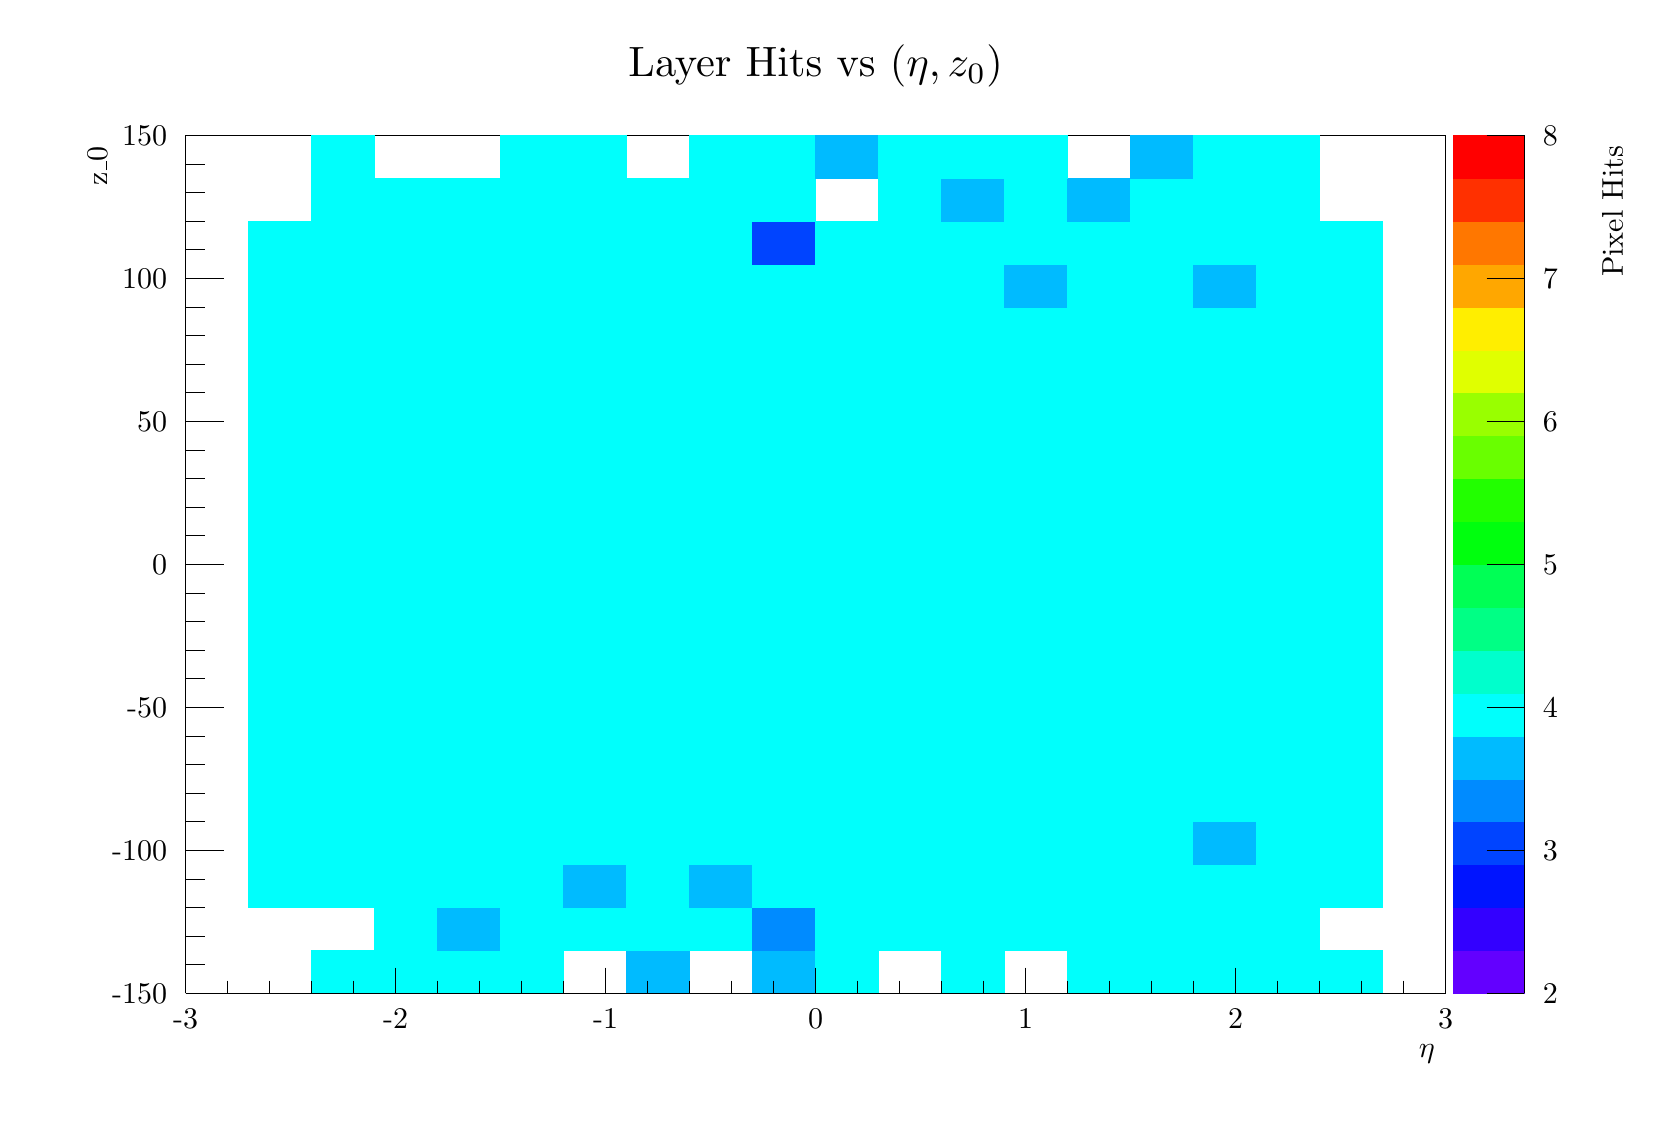
\begin{tikzpicture}
\pgfdeclareplotmark{cross} {
\pgfpathmoveto{\pgfpoint{-0.3\pgfplotmarksize}{\pgfplotmarksize}}
\pgfpathlineto{\pgfpoint{+0.3\pgfplotmarksize}{\pgfplotmarksize}}
\pgfpathlineto{\pgfpoint{+0.3\pgfplotmarksize}{0.3\pgfplotmarksize}}
\pgfpathlineto{\pgfpoint{+1\pgfplotmarksize}{0.3\pgfplotmarksize}}
\pgfpathlineto{\pgfpoint{+1\pgfplotmarksize}{-0.3\pgfplotmarksize}}
\pgfpathlineto{\pgfpoint{+0.3\pgfplotmarksize}{-0.3\pgfplotmarksize}}
\pgfpathlineto{\pgfpoint{+0.3\pgfplotmarksize}{-1.\pgfplotmarksize}}
\pgfpathlineto{\pgfpoint{-0.3\pgfplotmarksize}{-1.\pgfplotmarksize}}
\pgfpathlineto{\pgfpoint{-0.3\pgfplotmarksize}{-0.3\pgfplotmarksize}}
\pgfpathlineto{\pgfpoint{-1.\pgfplotmarksize}{-0.3\pgfplotmarksize}}
\pgfpathlineto{\pgfpoint{-1.\pgfplotmarksize}{0.3\pgfplotmarksize}}
\pgfpathlineto{\pgfpoint{-0.3\pgfplotmarksize}{0.3\pgfplotmarksize}}
\pgfpathclose
\pgfusepathqstroke
}
\pgfdeclareplotmark{cross*} {
\pgfpathmoveto{\pgfpoint{-0.3\pgfplotmarksize}{\pgfplotmarksize}}
\pgfpathlineto{\pgfpoint{+0.3\pgfplotmarksize}{\pgfplotmarksize}}
\pgfpathlineto{\pgfpoint{+0.3\pgfplotmarksize}{0.3\pgfplotmarksize}}
\pgfpathlineto{\pgfpoint{+1\pgfplotmarksize}{0.3\pgfplotmarksize}}
\pgfpathlineto{\pgfpoint{+1\pgfplotmarksize}{-0.3\pgfplotmarksize}}
\pgfpathlineto{\pgfpoint{+0.3\pgfplotmarksize}{-0.3\pgfplotmarksize}}
\pgfpathlineto{\pgfpoint{+0.3\pgfplotmarksize}{-1.\pgfplotmarksize}}
\pgfpathlineto{\pgfpoint{-0.3\pgfplotmarksize}{-1.\pgfplotmarksize}}
\pgfpathlineto{\pgfpoint{-0.3\pgfplotmarksize}{-0.3\pgfplotmarksize}}
\pgfpathlineto{\pgfpoint{-1.\pgfplotmarksize}{-0.3\pgfplotmarksize}}
\pgfpathlineto{\pgfpoint{-1.\pgfplotmarksize}{0.3\pgfplotmarksize}}
\pgfpathlineto{\pgfpoint{-0.3\pgfplotmarksize}{0.3\pgfplotmarksize}}
\pgfpathclose
\pgfusepathqfillstroke
}
\pgfdeclareplotmark{newstar} {
\pgfpathmoveto{\pgfqpoint{0pt}{\pgfplotmarksize}}
\pgfpathlineto{\pgfqpointpolar{44}{0.5\pgfplotmarksize}}
\pgfpathlineto{\pgfqpointpolar{18}{\pgfplotmarksize}}
\pgfpathlineto{\pgfqpointpolar{-20}{0.5\pgfplotmarksize}}
\pgfpathlineto{\pgfqpointpolar{-54}{\pgfplotmarksize}}
\pgfpathlineto{\pgfqpointpolar{-90}{0.5\pgfplotmarksize}}
\pgfpathlineto{\pgfqpointpolar{234}{\pgfplotmarksize}}
\pgfpathlineto{\pgfqpointpolar{198}{0.5\pgfplotmarksize}}
\pgfpathlineto{\pgfqpointpolar{162}{\pgfplotmarksize}}
\pgfpathlineto{\pgfqpointpolar{134}{0.5\pgfplotmarksize}}
\pgfpathclose
\pgfusepathqstroke
}
\pgfdeclareplotmark{newstar*} {
\pgfpathmoveto{\pgfqpoint{0pt}{\pgfplotmarksize}}
\pgfpathlineto{\pgfqpointpolar{44}{0.5\pgfplotmarksize}}
\pgfpathlineto{\pgfqpointpolar{18}{\pgfplotmarksize}}
\pgfpathlineto{\pgfqpointpolar{-20}{0.5\pgfplotmarksize}}
\pgfpathlineto{\pgfqpointpolar{-54}{\pgfplotmarksize}}
\pgfpathlineto{\pgfqpointpolar{-90}{0.5\pgfplotmarksize}}
\pgfpathlineto{\pgfqpointpolar{234}{\pgfplotmarksize}}
\pgfpathlineto{\pgfqpointpolar{198}{0.5\pgfplotmarksize}}
\pgfpathlineto{\pgfqpointpolar{162}{\pgfplotmarksize}}
\pgfpathlineto{\pgfqpointpolar{134}{0.5\pgfplotmarksize}}
\pgfpathclose
\pgfusepathqfillstroke
}
\definecolor{c}{rgb}{1,1,1};
\draw [color=c, fill=c] (0,0) rectangle (20,13.6207);
\draw [color=c, fill=c] (2,1.36207) rectangle (18,12.2586);
\definecolor{c}{rgb}{0,0,0};
\draw [c] (2,1.36207) -- (2,12.2586) -- (18,12.2586) -- (18,1.36207) -- (2,1.36207);
\definecolor{c}{rgb}{1,1,1};
\draw [color=c, fill=c] (2,1.36207) rectangle (18,12.2586);
\definecolor{c}{rgb}{0,0,0};
\draw [c] (2,1.36207) -- (2,12.2586) -- (18,12.2586) -- (18,1.36207) -- (2,1.36207);
\definecolor{c}{rgb}{0,1,0.986667};
\draw [color=c, fill=c] (3.6,1.36207) rectangle (4.4,1.9069);
\draw [color=c, fill=c] (4.4,1.36207) rectangle (5.2,1.9069);
\draw [color=c, fill=c] (5.2,1.36207) rectangle (6,1.9069);
\draw [color=c, fill=c] (6,1.36207) rectangle (6.8,1.9069);
\definecolor{c}{rgb}{0,0.733333,1};
\draw [color=c, fill=c] (7.6,1.36207) rectangle (8.4,1.9069);
\draw [color=c, fill=c] (9.2,1.36207) rectangle (10,1.9069);
\definecolor{c}{rgb}{0,1,0.986667};
\draw [color=c, fill=c] (10,1.36207) rectangle (10.8,1.9069);
\draw [color=c, fill=c] (11.6,1.36207) rectangle (12.4,1.9069);
\draw [color=c, fill=c] (13.2,1.36207) rectangle (14,1.9069);
\draw [color=c, fill=c] (14,1.36207) rectangle (14.8,1.9069);
\draw [color=c, fill=c] (14.8,1.36207) rectangle (15.6,1.9069);
\draw [color=c, fill=c] (15.6,1.36207) rectangle (16.4,1.9069);
\draw [color=c, fill=c] (16.4,1.36207) rectangle (17.2,1.9069);
\draw [color=c, fill=c] (4.4,1.9069) rectangle (5.2,2.45172);
\definecolor{c}{rgb}{0,0.733333,1};
\draw [color=c, fill=c] (5.2,1.9069) rectangle (6,2.45172);
\definecolor{c}{rgb}{0,1,0.986667};
\draw [color=c, fill=c] (6,1.9069) rectangle (6.8,2.45172);
\draw [color=c, fill=c] (6.8,1.9069) rectangle (7.6,2.45172);
\draw [color=c, fill=c] (7.6,1.9069) rectangle (8.4,2.45172);
\draw [color=c, fill=c] (8.4,1.9069) rectangle (9.2,2.45172);
\definecolor{c}{rgb}{0,0.546666,1};
\draw [color=c, fill=c] (9.2,1.9069) rectangle (10,2.45172);
\definecolor{c}{rgb}{0,1,0.986667};
\draw [color=c, fill=c] (10,1.9069) rectangle (10.8,2.45172);
\draw [color=c, fill=c] (10.8,1.9069) rectangle (11.6,2.45172);
\draw [color=c, fill=c] (11.6,1.9069) rectangle (12.4,2.45172);
\draw [color=c, fill=c] (12.4,1.9069) rectangle (13.2,2.45172);
\draw [color=c, fill=c] (13.2,1.9069) rectangle (14,2.45172);
\draw [color=c, fill=c] (14,1.9069) rectangle (14.8,2.45172);
\draw [color=c, fill=c] (14.8,1.9069) rectangle (15.6,2.45172);
\draw [color=c, fill=c] (15.6,1.9069) rectangle (16.4,2.45172);
\draw [color=c, fill=c] (2.8,2.45172) rectangle (3.6,2.99655);
\draw [color=c, fill=c] (3.6,2.45172) rectangle (4.4,2.99655);
\draw [color=c, fill=c] (4.4,2.45172) rectangle (5.2,2.99655);
\draw [color=c, fill=c] (5.2,2.45172) rectangle (6,2.99655);
\draw [color=c, fill=c] (6,2.45172) rectangle (6.8,2.99655);
\definecolor{c}{rgb}{0,0.733333,1};
\draw [color=c, fill=c] (6.8,2.45172) rectangle (7.6,2.99655);
\definecolor{c}{rgb}{0,1,0.986667};
\draw [color=c, fill=c] (7.6,2.45172) rectangle (8.4,2.99655);
\definecolor{c}{rgb}{0,0.733333,1};
\draw [color=c, fill=c] (8.4,2.45172) rectangle (9.2,2.99655);
\definecolor{c}{rgb}{0,1,0.986667};
\draw [color=c, fill=c] (9.2,2.45172) rectangle (10,2.99655);
\draw [color=c, fill=c] (10,2.45172) rectangle (10.8,2.99655);
\draw [color=c, fill=c] (10.8,2.45172) rectangle (11.6,2.99655);
\draw [color=c, fill=c] (11.6,2.45172) rectangle (12.4,2.99655);
\draw [color=c, fill=c] (12.4,2.45172) rectangle (13.2,2.99655);
\draw [color=c, fill=c] (13.2,2.45172) rectangle (14,2.99655);
\draw [color=c, fill=c] (14,2.45172) rectangle (14.8,2.99655);
\draw [color=c, fill=c] (14.8,2.45172) rectangle (15.6,2.99655);
\draw [color=c, fill=c] (15.6,2.45172) rectangle (16.4,2.99655);
\draw [color=c, fill=c] (16.4,2.45172) rectangle (17.2,2.99655);
\draw [color=c, fill=c] (2.8,2.99655) rectangle (3.6,3.54138);
\draw [color=c, fill=c] (3.6,2.99655) rectangle (4.4,3.54138);
\draw [color=c, fill=c] (4.4,2.99655) rectangle (5.2,3.54138);
\draw [color=c, fill=c] (5.2,2.99655) rectangle (6,3.54138);
\draw [color=c, fill=c] (6,2.99655) rectangle (6.8,3.54138);
\draw [color=c, fill=c] (6.8,2.99655) rectangle (7.6,3.54138);
\draw [color=c, fill=c] (7.6,2.99655) rectangle (8.4,3.54138);
\draw [color=c, fill=c] (8.4,2.99655) rectangle (9.2,3.54138);
\draw [color=c, fill=c] (9.2,2.99655) rectangle (10,3.54138);
\draw [color=c, fill=c] (10,2.99655) rectangle (10.8,3.54138);
\draw [color=c, fill=c] (10.8,2.99655) rectangle (11.6,3.54138);
\draw [color=c, fill=c] (11.6,2.99655) rectangle (12.4,3.54138);
\draw [color=c, fill=c] (12.4,2.99655) rectangle (13.2,3.54138);
\draw [color=c, fill=c] (13.2,2.99655) rectangle (14,3.54138);
\draw [color=c, fill=c] (14,2.99655) rectangle (14.8,3.54138);
\definecolor{c}{rgb}{0,0.733333,1};
\draw [color=c, fill=c] (14.8,2.99655) rectangle (15.6,3.54138);
\definecolor{c}{rgb}{0,1,0.986667};
\draw [color=c, fill=c] (15.6,2.99655) rectangle (16.4,3.54138);
\draw [color=c, fill=c] (16.4,2.99655) rectangle (17.2,3.54138);
\draw [color=c, fill=c] (2.8,3.54138) rectangle (3.6,4.08621);
\draw [color=c, fill=c] (3.6,3.54138) rectangle (4.4,4.08621);
\draw [color=c, fill=c] (4.4,3.54138) rectangle (5.2,4.08621);
\draw [color=c, fill=c] (5.2,3.54138) rectangle (6,4.08621);
\draw [color=c, fill=c] (6,3.54138) rectangle (6.8,4.08621);
\draw [color=c, fill=c] (6.8,3.54138) rectangle (7.6,4.08621);
\draw [color=c, fill=c] (7.6,3.54138) rectangle (8.4,4.08621);
\draw [color=c, fill=c] (8.4,3.54138) rectangle (9.2,4.08621);
\draw [color=c, fill=c] (9.2,3.54138) rectangle (10,4.08621);
\draw [color=c, fill=c] (10,3.54138) rectangle (10.8,4.08621);
\draw [color=c, fill=c] (10.8,3.54138) rectangle (11.6,4.08621);
\draw [color=c, fill=c] (11.6,3.54138) rectangle (12.4,4.08621);
\draw [color=c, fill=c] (12.4,3.54138) rectangle (13.2,4.08621);
\draw [color=c, fill=c] (13.2,3.54138) rectangle (14,4.08621);
\draw [color=c, fill=c] (14,3.54138) rectangle (14.8,4.08621);
\draw [color=c, fill=c] (14.8,3.54138) rectangle (15.6,4.08621);
\draw [color=c, fill=c] (15.6,3.54138) rectangle (16.4,4.08621);
\draw [color=c, fill=c] (16.4,3.54138) rectangle (17.2,4.08621);
\draw [color=c, fill=c] (2.8,4.08621) rectangle (3.6,4.63103);
\draw [color=c, fill=c] (3.6,4.08621) rectangle (4.4,4.63103);
\draw [color=c, fill=c] (4.4,4.08621) rectangle (5.2,4.63103);
\draw [color=c, fill=c] (5.2,4.08621) rectangle (6,4.63103);
\draw [color=c, fill=c] (6,4.08621) rectangle (6.8,4.63103);
\draw [color=c, fill=c] (6.8,4.08621) rectangle (7.6,4.63103);
\draw [color=c, fill=c] (7.6,4.08621) rectangle (8.4,4.63103);
\draw [color=c, fill=c] (8.4,4.08621) rectangle (9.2,4.63103);
\draw [color=c, fill=c] (9.2,4.08621) rectangle (10,4.63103);
\draw [color=c, fill=c] (10,4.08621) rectangle (10.8,4.63103);
\draw [color=c, fill=c] (10.8,4.08621) rectangle (11.6,4.63103);
\draw [color=c, fill=c] (11.6,4.08621) rectangle (12.4,4.63103);
\draw [color=c, fill=c] (12.4,4.08621) rectangle (13.2,4.63103);
\draw [color=c, fill=c] (13.2,4.08621) rectangle (14,4.63103);
\draw [color=c, fill=c] (14,4.08621) rectangle (14.8,4.63103);
\draw [color=c, fill=c] (14.8,4.08621) rectangle (15.6,4.63103);
\draw [color=c, fill=c] (15.6,4.08621) rectangle (16.4,4.63103);
\draw [color=c, fill=c] (16.4,4.08621) rectangle (17.2,4.63103);
\draw [color=c, fill=c] (2.8,4.63103) rectangle (3.6,5.17586);
\draw [color=c, fill=c] (3.6,4.63103) rectangle (4.4,5.17586);
\draw [color=c, fill=c] (4.4,4.63103) rectangle (5.2,5.17586);
\draw [color=c, fill=c] (5.2,4.63103) rectangle (6,5.17586);
\draw [color=c, fill=c] (6,4.63103) rectangle (6.8,5.17586);
\draw [color=c, fill=c] (6.8,4.63103) rectangle (7.6,5.17586);
\draw [color=c, fill=c] (7.6,4.63103) rectangle (8.4,5.17586);
\draw [color=c, fill=c] (8.4,4.63103) rectangle (9.2,5.17586);
\draw [color=c, fill=c] (9.2,4.63103) rectangle (10,5.17586);
\draw [color=c, fill=c] (10,4.63103) rectangle (10.8,5.17586);
\draw [color=c, fill=c] (10.8,4.63103) rectangle (11.6,5.17586);
\draw [color=c, fill=c] (11.6,4.63103) rectangle (12.4,5.17586);
\draw [color=c, fill=c] (12.4,4.63103) rectangle (13.2,5.17586);
\draw [color=c, fill=c] (13.2,4.63103) rectangle (14,5.17586);
\draw [color=c, fill=c] (14,4.63103) rectangle (14.8,5.17586);
\draw [color=c, fill=c] (14.8,4.63103) rectangle (15.6,5.17586);
\draw [color=c, fill=c] (15.6,4.63103) rectangle (16.4,5.17586);
\draw [color=c, fill=c] (16.4,4.63103) rectangle (17.2,5.17586);
\draw [color=c, fill=c] (2.8,5.17586) rectangle (3.6,5.72069);
\draw [color=c, fill=c] (3.6,5.17586) rectangle (4.4,5.72069);
\draw [color=c, fill=c] (4.4,5.17586) rectangle (5.2,5.72069);
\draw [color=c, fill=c] (5.2,5.17586) rectangle (6,5.72069);
\draw [color=c, fill=c] (6,5.17586) rectangle (6.8,5.72069);
\draw [color=c, fill=c] (6.8,5.17586) rectangle (7.6,5.72069);
\draw [color=c, fill=c] (7.6,5.17586) rectangle (8.4,5.72069);
\draw [color=c, fill=c] (8.4,5.17586) rectangle (9.2,5.72069);
\draw [color=c, fill=c] (9.2,5.17586) rectangle (10,5.72069);
\draw [color=c, fill=c] (10,5.17586) rectangle (10.8,5.72069);
\draw [color=c, fill=c] (10.8,5.17586) rectangle (11.6,5.72069);
\draw [color=c, fill=c] (11.6,5.17586) rectangle (12.4,5.72069);
\draw [color=c, fill=c] (12.4,5.17586) rectangle (13.2,5.72069);
\draw [color=c, fill=c] (13.2,5.17586) rectangle (14,5.72069);
\draw [color=c, fill=c] (14,5.17586) rectangle (14.8,5.72069);
\draw [color=c, fill=c] (14.8,5.17586) rectangle (15.6,5.72069);
\draw [color=c, fill=c] (15.6,5.17586) rectangle (16.4,5.72069);
\draw [color=c, fill=c] (16.4,5.17586) rectangle (17.2,5.72069);
\draw [color=c, fill=c] (2.8,5.72069) rectangle (3.6,6.26552);
\draw [color=c, fill=c] (3.6,5.72069) rectangle (4.4,6.26552);
\draw [color=c, fill=c] (4.4,5.72069) rectangle (5.2,6.26552);
\draw [color=c, fill=c] (5.2,5.72069) rectangle (6,6.26552);
\draw [color=c, fill=c] (6,5.72069) rectangle (6.8,6.26552);
\draw [color=c, fill=c] (6.8,5.72069) rectangle (7.6,6.26552);
\draw [color=c, fill=c] (7.6,5.72069) rectangle (8.4,6.26552);
\draw [color=c, fill=c] (8.4,5.72069) rectangle (9.2,6.26552);
\draw [color=c, fill=c] (9.2,5.72069) rectangle (10,6.26552);
\draw [color=c, fill=c] (10,5.72069) rectangle (10.8,6.26552);
\draw [color=c, fill=c] (10.8,5.72069) rectangle (11.6,6.26552);
\draw [color=c, fill=c] (11.6,5.72069) rectangle (12.4,6.26552);
\draw [color=c, fill=c] (12.4,5.72069) rectangle (13.2,6.26552);
\draw [color=c, fill=c] (13.2,5.72069) rectangle (14,6.26552);
\draw [color=c, fill=c] (14,5.72069) rectangle (14.8,6.26552);
\draw [color=c, fill=c] (14.8,5.72069) rectangle (15.6,6.26552);
\draw [color=c, fill=c] (15.6,5.72069) rectangle (16.4,6.26552);
\draw [color=c, fill=c] (16.4,5.72069) rectangle (17.2,6.26552);
\draw [color=c, fill=c] (2.8,6.26552) rectangle (3.6,6.81034);
\draw [color=c, fill=c] (3.6,6.26552) rectangle (4.4,6.81034);
\draw [color=c, fill=c] (4.4,6.26552) rectangle (5.2,6.81034);
\draw [color=c, fill=c] (5.2,6.26552) rectangle (6,6.81034);
\draw [color=c, fill=c] (6,6.26552) rectangle (6.8,6.81034);
\draw [color=c, fill=c] (6.8,6.26552) rectangle (7.6,6.81034);
\draw [color=c, fill=c] (7.6,6.26552) rectangle (8.4,6.81034);
\draw [color=c, fill=c] (8.4,6.26552) rectangle (9.2,6.81034);
\draw [color=c, fill=c] (9.2,6.26552) rectangle (10,6.81034);
\draw [color=c, fill=c] (10,6.26552) rectangle (10.8,6.81034);
\draw [color=c, fill=c] (10.8,6.26552) rectangle (11.6,6.81034);
\draw [color=c, fill=c] (11.6,6.26552) rectangle (12.4,6.81034);
\draw [color=c, fill=c] (12.4,6.26552) rectangle (13.2,6.81034);
\draw [color=c, fill=c] (13.2,6.26552) rectangle (14,6.81034);
\draw [color=c, fill=c] (14,6.26552) rectangle (14.8,6.81034);
\draw [color=c, fill=c] (14.8,6.26552) rectangle (15.6,6.81034);
\draw [color=c, fill=c] (15.6,6.26552) rectangle (16.4,6.81034);
\draw [color=c, fill=c] (16.4,6.26552) rectangle (17.2,6.81034);
\draw [color=c, fill=c] (2.8,6.81034) rectangle (3.6,7.35517);
\draw [color=c, fill=c] (3.6,6.81034) rectangle (4.4,7.35517);
\draw [color=c, fill=c] (4.4,6.81034) rectangle (5.2,7.35517);
\draw [color=c, fill=c] (5.2,6.81034) rectangle (6,7.35517);
\draw [color=c, fill=c] (6,6.81034) rectangle (6.8,7.35517);
\draw [color=c, fill=c] (6.8,6.81034) rectangle (7.6,7.35517);
\draw [color=c, fill=c] (7.6,6.81034) rectangle (8.4,7.35517);
\draw [color=c, fill=c] (8.4,6.81034) rectangle (9.2,7.35517);
\draw [color=c, fill=c] (9.2,6.81034) rectangle (10,7.35517);
\draw [color=c, fill=c] (10,6.81034) rectangle (10.8,7.35517);
\draw [color=c, fill=c] (10.8,6.81034) rectangle (11.6,7.35517);
\draw [color=c, fill=c] (11.6,6.81034) rectangle (12.4,7.35517);
\draw [color=c, fill=c] (12.4,6.81034) rectangle (13.2,7.35517);
\draw [color=c, fill=c] (13.2,6.81034) rectangle (14,7.35517);
\draw [color=c, fill=c] (14,6.81034) rectangle (14.8,7.35517);
\draw [color=c, fill=c] (14.8,6.81034) rectangle (15.6,7.35517);
\draw [color=c, fill=c] (15.6,6.81034) rectangle (16.4,7.35517);
\draw [color=c, fill=c] (16.4,6.81034) rectangle (17.2,7.35517);
\draw [color=c, fill=c] (2.8,7.35517) rectangle (3.6,7.9);
\draw [color=c, fill=c] (3.6,7.35517) rectangle (4.4,7.9);
\draw [color=c, fill=c] (4.4,7.35517) rectangle (5.2,7.9);
\draw [color=c, fill=c] (5.2,7.35517) rectangle (6,7.9);
\draw [color=c, fill=c] (6,7.35517) rectangle (6.8,7.9);
\draw [color=c, fill=c] (6.8,7.35517) rectangle (7.6,7.9);
\draw [color=c, fill=c] (7.6,7.35517) rectangle (8.4,7.9);
\draw [color=c, fill=c] (8.4,7.35517) rectangle (9.2,7.9);
\draw [color=c, fill=c] (9.2,7.35517) rectangle (10,7.9);
\draw [color=c, fill=c] (10,7.35517) rectangle (10.8,7.9);
\draw [color=c, fill=c] (10.8,7.35517) rectangle (11.6,7.9);
\draw [color=c, fill=c] (11.6,7.35517) rectangle (12.4,7.9);
\draw [color=c, fill=c] (12.4,7.35517) rectangle (13.2,7.9);
\draw [color=c, fill=c] (13.2,7.35517) rectangle (14,7.9);
\draw [color=c, fill=c] (14,7.35517) rectangle (14.8,7.9);
\draw [color=c, fill=c] (14.8,7.35517) rectangle (15.6,7.9);
\draw [color=c, fill=c] (15.6,7.35517) rectangle (16.4,7.9);
\draw [color=c, fill=c] (16.4,7.35517) rectangle (17.2,7.9);
\draw [color=c, fill=c] (2.8,7.9) rectangle (3.6,8.44483);
\draw [color=c, fill=c] (3.6,7.9) rectangle (4.4,8.44483);
\draw [color=c, fill=c] (4.4,7.9) rectangle (5.2,8.44483);
\draw [color=c, fill=c] (5.2,7.9) rectangle (6,8.44483);
\draw [color=c, fill=c] (6,7.9) rectangle (6.8,8.44483);
\draw [color=c, fill=c] (6.8,7.9) rectangle (7.6,8.44483);
\draw [color=c, fill=c] (7.6,7.9) rectangle (8.4,8.44483);
\draw [color=c, fill=c] (8.4,7.9) rectangle (9.2,8.44483);
\draw [color=c, fill=c] (9.2,7.9) rectangle (10,8.44483);
\draw [color=c, fill=c] (10,7.9) rectangle (10.8,8.44483);
\draw [color=c, fill=c] (10.8,7.9) rectangle (11.6,8.44483);
\draw [color=c, fill=c] (11.6,7.9) rectangle (12.4,8.44483);
\draw [color=c, fill=c] (12.4,7.9) rectangle (13.2,8.44483);
\draw [color=c, fill=c] (13.2,7.9) rectangle (14,8.44483);
\draw [color=c, fill=c] (14,7.9) rectangle (14.8,8.44483);
\draw [color=c, fill=c] (14.8,7.9) rectangle (15.6,8.44483);
\draw [color=c, fill=c] (15.6,7.9) rectangle (16.4,8.44483);
\draw [color=c, fill=c] (16.4,7.9) rectangle (17.2,8.44483);
\draw [color=c, fill=c] (2.8,8.44483) rectangle (3.6,8.98965);
\draw [color=c, fill=c] (3.6,8.44483) rectangle (4.4,8.98965);
\draw [color=c, fill=c] (4.4,8.44483) rectangle (5.2,8.98965);
\draw [color=c, fill=c] (5.2,8.44483) rectangle (6,8.98965);
\draw [color=c, fill=c] (6,8.44483) rectangle (6.8,8.98965);
\draw [color=c, fill=c] (6.8,8.44483) rectangle (7.6,8.98965);
\draw [color=c, fill=c] (7.6,8.44483) rectangle (8.4,8.98965);
\draw [color=c, fill=c] (8.4,8.44483) rectangle (9.2,8.98965);
\draw [color=c, fill=c] (9.2,8.44483) rectangle (10,8.98965);
\draw [color=c, fill=c] (10,8.44483) rectangle (10.8,8.98965);
\draw [color=c, fill=c] (10.8,8.44483) rectangle (11.6,8.98965);
\draw [color=c, fill=c] (11.6,8.44483) rectangle (12.4,8.98965);
\draw [color=c, fill=c] (12.4,8.44483) rectangle (13.2,8.98965);
\draw [color=c, fill=c] (13.2,8.44483) rectangle (14,8.98965);
\draw [color=c, fill=c] (14,8.44483) rectangle (14.8,8.98965);
\draw [color=c, fill=c] (14.8,8.44483) rectangle (15.6,8.98965);
\draw [color=c, fill=c] (15.6,8.44483) rectangle (16.4,8.98965);
\draw [color=c, fill=c] (16.4,8.44483) rectangle (17.2,8.98965);
\draw [color=c, fill=c] (2.8,8.98965) rectangle (3.6,9.53448);
\draw [color=c, fill=c] (3.6,8.98965) rectangle (4.4,9.53448);
\draw [color=c, fill=c] (4.4,8.98965) rectangle (5.2,9.53448);
\draw [color=c, fill=c] (5.2,8.98965) rectangle (6,9.53448);
\draw [color=c, fill=c] (6,8.98965) rectangle (6.8,9.53448);
\draw [color=c, fill=c] (6.8,8.98965) rectangle (7.6,9.53448);
\draw [color=c, fill=c] (7.6,8.98965) rectangle (8.4,9.53448);
\draw [color=c, fill=c] (8.4,8.98965) rectangle (9.2,9.53448);
\draw [color=c, fill=c] (9.2,8.98965) rectangle (10,9.53448);
\draw [color=c, fill=c] (10,8.98965) rectangle (10.8,9.53448);
\draw [color=c, fill=c] (10.8,8.98965) rectangle (11.6,9.53448);
\draw [color=c, fill=c] (11.6,8.98965) rectangle (12.4,9.53448);
\draw [color=c, fill=c] (12.4,8.98965) rectangle (13.2,9.53448);
\draw [color=c, fill=c] (13.2,8.98965) rectangle (14,9.53448);
\draw [color=c, fill=c] (14,8.98965) rectangle (14.8,9.53448);
\draw [color=c, fill=c] (14.8,8.98965) rectangle (15.6,9.53448);
\draw [color=c, fill=c] (15.6,8.98965) rectangle (16.4,9.53448);
\draw [color=c, fill=c] (16.4,8.98965) rectangle (17.2,9.53448);
\draw [color=c, fill=c] (2.8,9.53448) rectangle (3.6,10.0793);
\draw [color=c, fill=c] (3.6,9.53448) rectangle (4.4,10.0793);
\draw [color=c, fill=c] (4.4,9.53448) rectangle (5.2,10.0793);
\draw [color=c, fill=c] (5.2,9.53448) rectangle (6,10.0793);
\draw [color=c, fill=c] (6,9.53448) rectangle (6.8,10.0793);
\draw [color=c, fill=c] (6.8,9.53448) rectangle (7.6,10.0793);
\draw [color=c, fill=c] (7.6,9.53448) rectangle (8.4,10.0793);
\draw [color=c, fill=c] (8.4,9.53448) rectangle (9.2,10.0793);
\draw [color=c, fill=c] (9.2,9.53448) rectangle (10,10.0793);
\draw [color=c, fill=c] (10,9.53448) rectangle (10.8,10.0793);
\draw [color=c, fill=c] (10.8,9.53448) rectangle (11.6,10.0793);
\draw [color=c, fill=c] (11.6,9.53448) rectangle (12.4,10.0793);
\draw [color=c, fill=c] (12.4,9.53448) rectangle (13.2,10.0793);
\draw [color=c, fill=c] (13.2,9.53448) rectangle (14,10.0793);
\draw [color=c, fill=c] (14,9.53448) rectangle (14.8,10.0793);
\draw [color=c, fill=c] (14.8,9.53448) rectangle (15.6,10.0793);
\draw [color=c, fill=c] (15.6,9.53448) rectangle (16.4,10.0793);
\draw [color=c, fill=c] (16.4,9.53448) rectangle (17.2,10.0793);
\draw [color=c, fill=c] (2.8,10.0793) rectangle (3.6,10.6241);
\draw [color=c, fill=c] (3.6,10.0793) rectangle (4.4,10.6241);
\draw [color=c, fill=c] (4.4,10.0793) rectangle (5.2,10.6241);
\draw [color=c, fill=c] (5.2,10.0793) rectangle (6,10.6241);
\draw [color=c, fill=c] (6,10.0793) rectangle (6.8,10.6241);
\draw [color=c, fill=c] (6.8,10.0793) rectangle (7.6,10.6241);
\draw [color=c, fill=c] (7.6,10.0793) rectangle (8.4,10.6241);
\draw [color=c, fill=c] (8.4,10.0793) rectangle (9.2,10.6241);
\draw [color=c, fill=c] (9.2,10.0793) rectangle (10,10.6241);
\draw [color=c, fill=c] (10,10.0793) rectangle (10.8,10.6241);
\draw [color=c, fill=c] (10.8,10.0793) rectangle (11.6,10.6241);
\draw [color=c, fill=c] (11.6,10.0793) rectangle (12.4,10.6241);
\definecolor{c}{rgb}{0,0.733333,1};
\draw [color=c, fill=c] (12.4,10.0793) rectangle (13.2,10.6241);
\definecolor{c}{rgb}{0,1,0.986667};
\draw [color=c, fill=c] (13.2,10.0793) rectangle (14,10.6241);
\draw [color=c, fill=c] (14,10.0793) rectangle (14.8,10.6241);
\definecolor{c}{rgb}{0,0.733333,1};
\draw [color=c, fill=c] (14.8,10.0793) rectangle (15.6,10.6241);
\definecolor{c}{rgb}{0,1,0.986667};
\draw [color=c, fill=c] (15.6,10.0793) rectangle (16.4,10.6241);
\draw [color=c, fill=c] (16.4,10.0793) rectangle (17.2,10.6241);
\draw [color=c, fill=c] (2.8,10.6241) rectangle (3.6,11.169);
\draw [color=c, fill=c] (3.6,10.6241) rectangle (4.4,11.169);
\draw [color=c, fill=c] (4.4,10.6241) rectangle (5.2,11.169);
\draw [color=c, fill=c] (5.2,10.6241) rectangle (6,11.169);
\draw [color=c, fill=c] (6,10.6241) rectangle (6.8,11.169);
\draw [color=c, fill=c] (6.8,10.6241) rectangle (7.6,11.169);
\draw [color=c, fill=c] (7.6,10.6241) rectangle (8.4,11.169);
\draw [color=c, fill=c] (8.4,10.6241) rectangle (9.2,11.169);
\definecolor{c}{rgb}{0,0.266667,1};
\draw [color=c, fill=c] (9.2,10.6241) rectangle (10,11.169);
\definecolor{c}{rgb}{0,1,0.986667};
\draw [color=c, fill=c] (10,10.6241) rectangle (10.8,11.169);
\draw [color=c, fill=c] (10.8,10.6241) rectangle (11.6,11.169);
\draw [color=c, fill=c] (11.6,10.6241) rectangle (12.4,11.169);
\draw [color=c, fill=c] (12.4,10.6241) rectangle (13.2,11.169);
\draw [color=c, fill=c] (13.2,10.6241) rectangle (14,11.169);
\draw [color=c, fill=c] (14,10.6241) rectangle (14.8,11.169);
\draw [color=c, fill=c] (14.8,10.6241) rectangle (15.6,11.169);
\draw [color=c, fill=c] (15.6,10.6241) rectangle (16.4,11.169);
\draw [color=c, fill=c] (16.4,10.6241) rectangle (17.2,11.169);
\draw [color=c, fill=c] (3.6,11.169) rectangle (4.4,11.7138);
\draw [color=c, fill=c] (4.4,11.169) rectangle (5.2,11.7138);
\draw [color=c, fill=c] (5.2,11.169) rectangle (6,11.7138);
\draw [color=c, fill=c] (6,11.169) rectangle (6.8,11.7138);
\draw [color=c, fill=c] (6.8,11.169) rectangle (7.6,11.7138);
\draw [color=c, fill=c] (7.6,11.169) rectangle (8.4,11.7138);
\draw [color=c, fill=c] (8.4,11.169) rectangle (9.2,11.7138);
\draw [color=c, fill=c] (9.2,11.169) rectangle (10,11.7138);
\draw [color=c, fill=c] (10.8,11.169) rectangle (11.6,11.7138);
\definecolor{c}{rgb}{0,0.733333,1};
\draw [color=c, fill=c] (11.6,11.169) rectangle (12.4,11.7138);
\definecolor{c}{rgb}{0,1,0.986667};
\draw [color=c, fill=c] (12.4,11.169) rectangle (13.2,11.7138);
\definecolor{c}{rgb}{0,0.733333,1};
\draw [color=c, fill=c] (13.2,11.169) rectangle (14,11.7138);
\definecolor{c}{rgb}{0,1,0.986667};
\draw [color=c, fill=c] (14,11.169) rectangle (14.8,11.7138);
\draw [color=c, fill=c] (14.8,11.169) rectangle (15.6,11.7138);
\draw [color=c, fill=c] (15.6,11.169) rectangle (16.4,11.7138);
\draw [color=c, fill=c] (3.6,11.7138) rectangle (4.4,12.2586);
\draw [color=c, fill=c] (6,11.7138) rectangle (6.8,12.2586);
\draw [color=c, fill=c] (6.8,11.7138) rectangle (7.6,12.2586);
\draw [color=c, fill=c] (8.4,11.7138) rectangle (9.2,12.2586);
\draw [color=c, fill=c] (9.2,11.7138) rectangle (10,12.2586);
\definecolor{c}{rgb}{0,0.733333,1};
\draw [color=c, fill=c] (10,11.7138) rectangle (10.8,12.2586);
\definecolor{c}{rgb}{0,1,0.986667};
\draw [color=c, fill=c] (10.8,11.7138) rectangle (11.6,12.2586);
\draw [color=c, fill=c] (11.6,11.7138) rectangle (12.4,12.2586);
\draw [color=c, fill=c] (12.4,11.7138) rectangle (13.2,12.2586);
\definecolor{c}{rgb}{0,0.733333,1};
\draw [color=c, fill=c] (14,11.7138) rectangle (14.8,12.2586);
\definecolor{c}{rgb}{0,1,0.986667};
\draw [color=c, fill=c] (14.8,11.7138) rectangle (15.6,12.2586);
\draw [color=c, fill=c] (15.6,11.7138) rectangle (16.4,12.2586);
\definecolor{c}{rgb}{0,0,0};
\draw [c] (2,1.36207) -- (18,1.36207);
\draw [anchor= east] (18,0.59931) node[scale=1.08496, color=c, rotate=0]{$\eta$};
\draw [c] (2,1.68897) -- (2,1.36207);
\draw [c] (2.53333,1.52552) -- (2.53333,1.36207);
\draw [c] (3.06667,1.52552) -- (3.06667,1.36207);
\draw [c] (3.6,1.52552) -- (3.6,1.36207);
\draw [c] (4.13333,1.52552) -- (4.13333,1.36207);
\draw [c] (4.66667,1.68897) -- (4.66667,1.36207);
\draw [c] (5.2,1.52552) -- (5.2,1.36207);
\draw [c] (5.73333,1.52552) -- (5.73333,1.36207);
\draw [c] (6.26667,1.52552) -- (6.26667,1.36207);
\draw [c] (6.8,1.52552) -- (6.8,1.36207);
\draw [c] (7.33333,1.68897) -- (7.33333,1.36207);
\draw [c] (7.86667,1.52552) -- (7.86667,1.36207);
\draw [c] (8.4,1.52552) -- (8.4,1.36207);
\draw [c] (8.93333,1.52552) -- (8.93333,1.36207);
\draw [c] (9.46667,1.52552) -- (9.46667,1.36207);
\draw [c] (10,1.68897) -- (10,1.36207);
\draw [c] (10.5333,1.52552) -- (10.5333,1.36207);
\draw [c] (11.0667,1.52552) -- (11.0667,1.36207);
\draw [c] (11.6,1.52552) -- (11.6,1.36207);
\draw [c] (12.1333,1.52552) -- (12.1333,1.36207);
\draw [c] (12.6667,1.68897) -- (12.6667,1.36207);
\draw [c] (13.2,1.52552) -- (13.2,1.36207);
\draw [c] (13.7333,1.52552) -- (13.7333,1.36207);
\draw [c] (14.2667,1.52552) -- (14.2667,1.36207);
\draw [c] (14.8,1.52552) -- (14.8,1.36207);
\draw [c] (15.3333,1.68897) -- (15.3333,1.36207);
\draw [c] (15.8667,1.52552) -- (15.8667,1.36207);
\draw [c] (16.4,1.52552) -- (16.4,1.36207);
\draw [c] (16.9333,1.52552) -- (16.9333,1.36207);
\draw [c] (17.4667,1.52552) -- (17.4667,1.36207);
\draw [c] (18,1.68897) -- (18,1.36207);
\draw [anchor=base] (2,0.912586) node[scale=1.08496, color=c, rotate=0]{-3};
\draw [anchor=base] (4.66667,0.912586) node[scale=1.08496, color=c, rotate=0]{-2};
\draw [anchor=base] (7.33333,0.912586) node[scale=1.08496, color=c, rotate=0]{-1};
\draw [anchor=base] (10,0.912586) node[scale=1.08496, color=c, rotate=0]{0};
\draw [anchor=base] (12.6667,0.912586) node[scale=1.08496, color=c, rotate=0]{1};
\draw [anchor=base] (15.3333,0.912586) node[scale=1.08496, color=c, rotate=0]{2};
\draw [anchor=base] (18,0.912586) node[scale=1.08496, color=c, rotate=0]{3};
\draw [c] (2,1.36207) -- (2,12.2586);
\draw [anchor= east] (0.88,12.2586) node[scale=1.08496, color=c, rotate=90]{z\_{0}};
\draw [c] (2.48,1.36207) -- (2,1.36207);
\draw [c] (2.24,1.72529) -- (2,1.72529);
\draw [c] (2.24,2.08851) -- (2,2.08851);
\draw [c] (2.24,2.45172) -- (2,2.45172);
\draw [c] (2.24,2.81494) -- (2,2.81494);
\draw [c] (2.48,3.17816) -- (2,3.17816);
\draw [c] (2.24,3.54138) -- (2,3.54138);
\draw [c] (2.24,3.9046) -- (2,3.9046);
\draw [c] (2.24,4.26782) -- (2,4.26782);
\draw [c] (2.24,4.63103) -- (2,4.63103);
\draw [c] (2.48,4.99425) -- (2,4.99425);
\draw [c] (2.24,5.35747) -- (2,5.35747);
\draw [c] (2.24,5.72069) -- (2,5.72069);
\draw [c] (2.24,6.08391) -- (2,6.08391);
\draw [c] (2.24,6.44713) -- (2,6.44713);
\draw [c] (2.48,6.81034) -- (2,6.81034);
\draw [c] (2.24,7.17356) -- (2,7.17356);
\draw [c] (2.24,7.53678) -- (2,7.53678);
\draw [c] (2.24,7.9) -- (2,7.9);
\draw [c] (2.24,8.26322) -- (2,8.26322);
\draw [c] (2.48,8.62644) -- (2,8.62644);
\draw [c] (2.24,8.98965) -- (2,8.98965);
\draw [c] (2.24,9.35287) -- (2,9.35287);
\draw [c] (2.24,9.71609) -- (2,9.71609);
\draw [c] (2.24,10.0793) -- (2,10.0793);
\draw [c] (2.48,10.4425) -- (2,10.4425);
\draw [c] (2.24,10.8057) -- (2,10.8057);
\draw [c] (2.24,11.169) -- (2,11.169);
\draw [c] (2.24,11.5322) -- (2,11.5322);
\draw [c] (2.24,11.8954) -- (2,11.8954);
\draw [c] (2.48,12.2586) -- (2,12.2586);
\draw [anchor= east] (1.9,1.36207) node[scale=1.08496, color=c, rotate=0]{-150};
\draw [anchor= east] (1.9,3.17816) node[scale=1.08496, color=c, rotate=0]{-100};
\draw [anchor= east] (1.9,4.99425) node[scale=1.08496, color=c, rotate=0]{-50};
\draw [anchor= east] (1.9,6.81034) node[scale=1.08496, color=c, rotate=0]{0};
\draw [anchor= east] (1.9,8.62644) node[scale=1.08496, color=c, rotate=0]{50};
\draw [anchor= east] (1.9,10.4425) node[scale=1.08496, color=c, rotate=0]{100};
\draw [anchor= east] (1.9,12.2586) node[scale=1.08496, color=c, rotate=0]{150};
\definecolor{c}{rgb}{0.386667,0,1};
\draw [color=c, fill=c] (18.1,1.36207) rectangle (19,1.9069);
\definecolor{c}{rgb}{0.2,0,1};
\draw [color=c, fill=c] (18.1,1.9069) rectangle (19,2.45172);
\definecolor{c}{rgb}{0,0.0800001,1};
\draw [color=c, fill=c] (18.1,2.45172) rectangle (19,2.99655);
\definecolor{c}{rgb}{0,0.266667,1};
\draw [color=c, fill=c] (18.1,2.99655) rectangle (19,3.54138);
\definecolor{c}{rgb}{0,0.546666,1};
\draw [color=c, fill=c] (18.1,3.54138) rectangle (19,4.08621);
\definecolor{c}{rgb}{0,0.733333,1};
\draw [color=c, fill=c] (18.1,4.08621) rectangle (19,4.63103);
\definecolor{c}{rgb}{0,1,0.986667};
\draw [color=c, fill=c] (18.1,4.63103) rectangle (19,5.17586);
\definecolor{c}{rgb}{0,1,0.8};
\draw [color=c, fill=c] (18.1,5.17586) rectangle (19,5.72069);
\definecolor{c}{rgb}{0,1,0.52};
\draw [color=c, fill=c] (18.1,5.72069) rectangle (19,6.26552);
\definecolor{c}{rgb}{0,1,0.333333};
\draw [color=c, fill=c] (18.1,6.26552) rectangle (19,6.81034);
\definecolor{c}{rgb}{0,1,0.0533333};
\draw [color=c, fill=c] (18.1,6.81034) rectangle (19,7.35517);
\definecolor{c}{rgb}{0.133333,1,0};
\draw [color=c, fill=c] (18.1,7.35517) rectangle (19,7.9);
\definecolor{c}{rgb}{0.413333,1,0};
\draw [color=c, fill=c] (18.1,7.9) rectangle (19,8.44483);
\definecolor{c}{rgb}{0.6,1,0};
\draw [color=c, fill=c] (18.1,8.44483) rectangle (19,8.98965);
\definecolor{c}{rgb}{0.88,1,0};
\draw [color=c, fill=c] (18.1,8.98965) rectangle (19,9.53448);
\definecolor{c}{rgb}{1,0.933333,0};
\draw [color=c, fill=c] (18.1,9.53448) rectangle (19,10.0793);
\definecolor{c}{rgb}{1,0.653333,0};
\draw [color=c, fill=c] (18.1,10.0793) rectangle (19,10.6241);
\definecolor{c}{rgb}{1,0.466667,0};
\draw [color=c, fill=c] (18.1,10.6241) rectangle (19,11.169);
\definecolor{c}{rgb}{1,0.186667,0};
\draw [color=c, fill=c] (18.1,11.169) rectangle (19,11.7138);
\definecolor{c}{rgb}{1,0,0};
\draw [color=c, fill=c] (18.1,11.7138) rectangle (19,12.2586);
\definecolor{c}{rgb}{0,0,0};
\draw [c] (19,1.36207) -- (19,12.2586);
\draw [anchor= east] (20.12,12.2586) node[scale=1.08496, color=c, rotate=90]{$\mbox{Pixel Hits}$};
\draw [c] (18.52,1.36207) -- (19,1.36207);
\draw [c] (18.52,3.17816) -- (19,3.17816);
\draw [c] (18.52,4.99425) -- (19,4.99425);
\draw [c] (18.52,6.81034) -- (19,6.81034);
\draw [c] (18.52,8.62644) -- (19,8.62644);
\draw [c] (18.52,10.4425) -- (19,10.4425);
\draw [c] (18.52,12.2586) -- (19,12.2586);
\draw [anchor= west] (19.1,1.36207) node[scale=1.08496, color=c, rotate=0]{2};
\draw [anchor= west] (19.1,3.17816) node[scale=1.08496, color=c, rotate=0]{3};
\draw [anchor= west] (19.1,4.99425) node[scale=1.08496, color=c, rotate=0]{4};
\draw [anchor= west] (19.1,6.81034) node[scale=1.08496, color=c, rotate=0]{5};
\draw [anchor= west] (19.1,8.62644) node[scale=1.08496, color=c, rotate=0]{6};
\draw [anchor= west] (19.1,10.4425) node[scale=1.08496, color=c, rotate=0]{7};
\draw [anchor= west] (19.1,12.2586) node[scale=1.08496, color=c, rotate=0]{8};
\draw (10,13.1388) node[scale=1.5317, color=c, rotate=0]{$\mbox{Layer Hits vs }(\eta,z_{0})$};
\end{tikzpicture}
}
\end{subfigure}
\caption{Layer hits vs $(\eta, z)$.}
\end{figure}

\begin{figure}[H]
\centering
 \resizebox{.8\linewidth}{!}{\begin{tikzpicture}
\pgfdeclareplotmark{cross} {
\pgfpathmoveto{\pgfpoint{-0.3\pgfplotmarksize}{\pgfplotmarksize}}
\pgfpathlineto{\pgfpoint{+0.3\pgfplotmarksize}{\pgfplotmarksize}}
\pgfpathlineto{\pgfpoint{+0.3\pgfplotmarksize}{0.3\pgfplotmarksize}}
\pgfpathlineto{\pgfpoint{+1\pgfplotmarksize}{0.3\pgfplotmarksize}}
\pgfpathlineto{\pgfpoint{+1\pgfplotmarksize}{-0.3\pgfplotmarksize}}
\pgfpathlineto{\pgfpoint{+0.3\pgfplotmarksize}{-0.3\pgfplotmarksize}}
\pgfpathlineto{\pgfpoint{+0.3\pgfplotmarksize}{-1.\pgfplotmarksize}}
\pgfpathlineto{\pgfpoint{-0.3\pgfplotmarksize}{-1.\pgfplotmarksize}}
\pgfpathlineto{\pgfpoint{-0.3\pgfplotmarksize}{-0.3\pgfplotmarksize}}
\pgfpathlineto{\pgfpoint{-1.\pgfplotmarksize}{-0.3\pgfplotmarksize}}
\pgfpathlineto{\pgfpoint{-1.\pgfplotmarksize}{0.3\pgfplotmarksize}}
\pgfpathlineto{\pgfpoint{-0.3\pgfplotmarksize}{0.3\pgfplotmarksize}}
\pgfpathclose
\pgfusepathqstroke
}
\pgfdeclareplotmark{cross*} {
\pgfpathmoveto{\pgfpoint{-0.3\pgfplotmarksize}{\pgfplotmarksize}}
\pgfpathlineto{\pgfpoint{+0.3\pgfplotmarksize}{\pgfplotmarksize}}
\pgfpathlineto{\pgfpoint{+0.3\pgfplotmarksize}{0.3\pgfplotmarksize}}
\pgfpathlineto{\pgfpoint{+1\pgfplotmarksize}{0.3\pgfplotmarksize}}
\pgfpathlineto{\pgfpoint{+1\pgfplotmarksize}{-0.3\pgfplotmarksize}}
\pgfpathlineto{\pgfpoint{+0.3\pgfplotmarksize}{-0.3\pgfplotmarksize}}
\pgfpathlineto{\pgfpoint{+0.3\pgfplotmarksize}{-1.\pgfplotmarksize}}
\pgfpathlineto{\pgfpoint{-0.3\pgfplotmarksize}{-1.\pgfplotmarksize}}
\pgfpathlineto{\pgfpoint{-0.3\pgfplotmarksize}{-0.3\pgfplotmarksize}}
\pgfpathlineto{\pgfpoint{-1.\pgfplotmarksize}{-0.3\pgfplotmarksize}}
\pgfpathlineto{\pgfpoint{-1.\pgfplotmarksize}{0.3\pgfplotmarksize}}
\pgfpathlineto{\pgfpoint{-0.3\pgfplotmarksize}{0.3\pgfplotmarksize}}
\pgfpathclose
\pgfusepathqfillstroke
}
\pgfdeclareplotmark{newstar} {
\pgfpathmoveto{\pgfqpoint{0pt}{\pgfplotmarksize}}
\pgfpathlineto{\pgfqpointpolar{44}{0.5\pgfplotmarksize}}
\pgfpathlineto{\pgfqpointpolar{18}{\pgfplotmarksize}}
\pgfpathlineto{\pgfqpointpolar{-20}{0.5\pgfplotmarksize}}
\pgfpathlineto{\pgfqpointpolar{-54}{\pgfplotmarksize}}
\pgfpathlineto{\pgfqpointpolar{-90}{0.5\pgfplotmarksize}}
\pgfpathlineto{\pgfqpointpolar{234}{\pgfplotmarksize}}
\pgfpathlineto{\pgfqpointpolar{198}{0.5\pgfplotmarksize}}
\pgfpathlineto{\pgfqpointpolar{162}{\pgfplotmarksize}}
\pgfpathlineto{\pgfqpointpolar{134}{0.5\pgfplotmarksize}}
\pgfpathclose
\pgfusepathqstroke
}
\pgfdeclareplotmark{newstar*} {
\pgfpathmoveto{\pgfqpoint{0pt}{\pgfplotmarksize}}
\pgfpathlineto{\pgfqpointpolar{44}{0.5\pgfplotmarksize}}
\pgfpathlineto{\pgfqpointpolar{18}{\pgfplotmarksize}}
\pgfpathlineto{\pgfqpointpolar{-20}{0.5\pgfplotmarksize}}
\pgfpathlineto{\pgfqpointpolar{-54}{\pgfplotmarksize}}
\pgfpathlineto{\pgfqpointpolar{-90}{0.5\pgfplotmarksize}}
\pgfpathlineto{\pgfqpointpolar{234}{\pgfplotmarksize}}
\pgfpathlineto{\pgfqpointpolar{198}{0.5\pgfplotmarksize}}
\pgfpathlineto{\pgfqpointpolar{162}{\pgfplotmarksize}}
\pgfpathlineto{\pgfqpointpolar{134}{0.5\pgfplotmarksize}}
\pgfpathclose
\pgfusepathqfillstroke
}
\definecolor{c}{rgb}{1,1,1};
\draw [color=c, fill=c] (0,0) rectangle (20,13.6207);
\draw [color=c, fill=c] (2,1.36207) rectangle (18,12.2586);
\definecolor{c}{rgb}{0,0,0};
\draw [c] (2,1.36207) -- (2,12.2586) -- (18,12.2586) -- (18,1.36207) -- (2,1.36207);
\definecolor{c}{rgb}{1,1,1};
\draw [color=c, fill=c] (2,1.36207) rectangle (18,12.2586);
\definecolor{c}{rgb}{0,0,0};
\draw [c] (2,1.36207) -- (2,12.2586) -- (18,12.2586) -- (18,1.36207) -- (2,1.36207);
\definecolor{c}{rgb}{1,0,0};
\draw [c] (2.5,6.66917) -- (2.63506,6.66917);
\draw [c] (2.86494,6.66917) -- (3,6.66917);
\foreach \P in {(2.75,6.66917)}{\draw[mark options={color=c,fill=c},mark size=2.402402pt,mark=*] plot coordinates {\P};}
\draw [c] (3,6.62881) -- (3.13506,6.62881);
\draw [c] (3.36494,6.62881) -- (3.5,6.62881);
\foreach \P in {(3.25,6.62881)}{\draw[mark options={color=c,fill=c},mark size=2.402402pt,mark=*] plot coordinates {\P};}
\draw [c] (3.5,6.6415) -- (3.63506,6.6415);
\draw [c] (3.86494,6.6415) -- (4,6.6415);
\foreach \P in {(3.75,6.6415)}{\draw[mark options={color=c,fill=c},mark size=2.402402pt,mark=*] plot coordinates {\P};}
\draw [c] (4,6.69697) -- (4.13506,6.69697);
\draw [c] (4.36494,6.69697) -- (4.5,6.69697);
\foreach \P in {(4.25,6.69697)}{\draw[mark options={color=c,fill=c},mark size=2.402402pt,mark=*] plot coordinates {\P};}
\draw [c] (4.5,6.68136) -- (4.63506,6.68136);
\draw [c] (4.86494,6.68136) -- (5,6.68136);
\foreach \P in {(4.75,6.68136)}{\draw[mark options={color=c,fill=c},mark size=2.402402pt,mark=*] plot coordinates {\P};}
\draw [c] (5,6.65463) -- (5.13506,6.65463);
\draw [c] (5.36494,6.65463) -- (5.5,6.65463);
\foreach \P in {(5.25,6.65463)}{\draw[mark options={color=c,fill=c},mark size=2.402402pt,mark=*] plot coordinates {\P};}
\draw [c] (5.5,6.6842) -- (5.63506,6.6842);
\draw [c] (5.86494,6.6842) -- (6,6.6842);
\foreach \P in {(5.75,6.6842)}{\draw[mark options={color=c,fill=c},mark size=2.402402pt,mark=*] plot coordinates {\P};}
\draw [c] (6,6.66741) -- (6.13506,6.66741);
\draw [c] (6.36494,6.66741) -- (6.5,6.66741);
\foreach \P in {(6.25,6.66741)}{\draw[mark options={color=c,fill=c},mark size=2.402402pt,mark=*] plot coordinates {\P};}
\draw [c] (6.5,6.66841) -- (6.63506,6.66841);
\draw [c] (6.86494,6.66841) -- (7,6.66841);
\foreach \P in {(6.75,6.66841)}{\draw[mark options={color=c,fill=c},mark size=2.402402pt,mark=*] plot coordinates {\P};}
\draw [c] (7,6.66863) -- (7.13506,6.66863);
\draw [c] (7.36494,6.66863) -- (7.5,6.66863);
\foreach \P in {(7.25,6.66863)}{\draw[mark options={color=c,fill=c},mark size=2.402402pt,mark=*] plot coordinates {\P};}
\draw [c] (7.5,6.66937) -- (7.63506,6.66937);
\draw [c] (7.86494,6.66937) -- (8,6.66937);
\foreach \P in {(7.75,6.66937)}{\draw[mark options={color=c,fill=c},mark size=2.402402pt,mark=*] plot coordinates {\P};}
\draw [c] (8,6.79502) -- (8.13506,6.79502);
\draw [c] (8.36494,6.79502) -- (8.5,6.79502);
\foreach \P in {(8.25,6.79502)}{\draw[mark options={color=c,fill=c},mark size=2.402402pt,mark=*] plot coordinates {\P};}
\draw [c] (8.5,11.6789) -- (8.63506,11.6789);
\draw [c] (8.86494,11.6789) -- (9,11.6789);
\foreach \P in {(8.75,11.6789)}{\draw[mark options={color=c,fill=c},mark size=2.402402pt,mark=*] plot coordinates {\P};}
\draw [c] (9.25,8.26073) -- (9.25,8.27565);
\draw [c] (9.25,8.50553) -- (9.25,8.52045);
\draw [c] (9,8.39059) -- (9.13506,8.39059);
\draw [c] (9.36494,8.39059) -- (9.5,8.39059);
\foreach \P in {(9.25,8.39059)}{\draw[mark options={color=c,fill=c},mark size=2.402402pt,mark=*] plot coordinates {\P};}
\draw [c] (9.5,6.64036) -- (9.63506,6.64036);
\draw [c] (9.86494,6.64036) -- (10,6.64036);
\foreach \P in {(9.75,6.64036)}{\draw[mark options={color=c,fill=c},mark size=2.402402pt,mark=*] plot coordinates {\P};}
\draw [c] (10,6.66867) -- (10.1351,6.66867);
\draw [c] (10.3649,6.66867) -- (10.5,6.66867);
\foreach \P in {(10.25,6.66867)}{\draw[mark options={color=c,fill=c},mark size=2.402402pt,mark=*] plot coordinates {\P};}
\draw [c] (10.5,6.65463) -- (10.6351,6.65463);
\draw [c] (10.8649,6.65463) -- (11,6.65463);
\foreach \P in {(10.75,6.65463)}{\draw[mark options={color=c,fill=c},mark size=2.402402pt,mark=*] plot coordinates {\P};}
\draw [c] (11,6.66852) -- (11.1351,6.66852);
\draw [c] (11.3649,6.66852) -- (11.5,6.66852);
\foreach \P in {(11.25,6.66852)}{\draw[mark options={color=c,fill=c},mark size=2.402402pt,mark=*] plot coordinates {\P};}
\draw [c] (11.5,6.66711) -- (11.6351,6.66711);
\draw [c] (11.8649,6.66711) -- (12,6.66711);
\foreach \P in {(11.75,6.66711)}{\draw[mark options={color=c,fill=c},mark size=2.402402pt,mark=*] plot coordinates {\P};}
\draw [c] (12,6.66776) -- (12.1351,6.66776);
\draw [c] (12.3649,6.66776) -- (12.5,6.66776);
\foreach \P in {(12.25,6.66776)}{\draw[mark options={color=c,fill=c},mark size=2.402402pt,mark=*] plot coordinates {\P};}
\draw [c] (12.5,6.66717) -- (12.6351,6.66717);
\draw [c] (12.8649,6.66717) -- (13,6.66717);
\foreach \P in {(12.75,6.66717)}{\draw[mark options={color=c,fill=c},mark size=2.402402pt,mark=*] plot coordinates {\P};}
\draw [c] (13,6.65463) -- (13.1351,6.65463);
\draw [c] (13.3649,6.65463) -- (13.5,6.65463);
\foreach \P in {(13.25,6.65463)}{\draw[mark options={color=c,fill=c},mark size=2.402402pt,mark=*] plot coordinates {\P};}
\draw [c] (13.5,6.65463) -- (13.6351,6.65463);
\draw [c] (13.8649,6.65463) -- (14,6.65463);
\foreach \P in {(13.75,6.65463)}{\draw[mark options={color=c,fill=c},mark size=2.402402pt,mark=*] plot coordinates {\P};}
\draw [c] (14,6.68191) -- (14.1351,6.68191);
\draw [c] (14.3649,6.68191) -- (14.5,6.68191);
\foreach \P in {(14.25,6.68191)}{\draw[mark options={color=c,fill=c},mark size=2.402402pt,mark=*] plot coordinates {\P};}
\draw [c] (14.5,6.65463) -- (14.6351,6.65463);
\draw [c] (14.8649,6.65463) -- (15,6.65463);
\foreach \P in {(14.75,6.65463)}{\draw[mark options={color=c,fill=c},mark size=2.402402pt,mark=*] plot coordinates {\P};}
\draw [c] (15,6.61433) -- (15.1351,6.61433);
\draw [c] (15.3649,6.61433) -- (15.5,6.61433);
\foreach \P in {(15.25,6.61433)}{\draw[mark options={color=c,fill=c},mark size=2.402402pt,mark=*] plot coordinates {\P};}
\draw [c] (15.5,6.64113) -- (15.6351,6.64113);
\draw [c] (15.8649,6.64113) -- (16,6.64113);
\foreach \P in {(15.75,6.64113)}{\draw[mark options={color=c,fill=c},mark size=2.402402pt,mark=*] plot coordinates {\P};}
\draw [c] (16,6.65463) -- (16.1351,6.65463);
\draw [c] (16.3649,6.65463) -- (16.5,6.65463);
\foreach \P in {(16.25,6.65463)}{\draw[mark options={color=c,fill=c},mark size=2.402402pt,mark=*] plot coordinates {\P};}
\draw [c] (16.5,6.65463) -- (16.6351,6.65463);
\draw [c] (16.8649,6.65463) -- (17,6.65463);
\foreach \P in {(16.75,6.65463)}{\draw[mark options={color=c,fill=c},mark size=2.402402pt,mark=*] plot coordinates {\P};}
\draw [c] (17,6.70919) -- (17.1351,6.70919);
\draw [c] (17.3649,6.70919) -- (17.5,6.70919);
\foreach \P in {(17.25,6.70919)}{\draw[mark options={color=c,fill=c},mark size=2.402402pt,mark=*] plot coordinates {\P};}
\definecolor{c}{rgb}{0,0,0};
\draw [c] (2,1.36207) -- (18,1.36207);
\draw [anchor= east] (18,0.59931) node[scale=1.08496, color=c, rotate=0]{$\phi$};
\draw [c] (2.5,1.68897) -- (2.5,1.36207);
\draw [c] (2.875,1.52552) -- (2.875,1.36207);
\draw [c] (3.25,1.52552) -- (3.25,1.36207);
\draw [c] (3.625,1.52552) -- (3.625,1.36207);
\draw [c] (4,1.52552) -- (4,1.36207);
\draw [c] (4.375,1.68897) -- (4.375,1.36207);
\draw [c] (4.75,1.52552) -- (4.75,1.36207);
\draw [c] (5.125,1.52552) -- (5.125,1.36207);
\draw [c] (5.5,1.52552) -- (5.5,1.36207);
\draw [c] (5.875,1.52552) -- (5.875,1.36207);
\draw [c] (6.25,1.68897) -- (6.25,1.36207);
\draw [c] (6.625,1.52552) -- (6.625,1.36207);
\draw [c] (7,1.52552) -- (7,1.36207);
\draw [c] (7.375,1.52552) -- (7.375,1.36207);
\draw [c] (7.75,1.52552) -- (7.75,1.36207);
\draw [c] (8.125,1.68897) -- (8.125,1.36207);
\draw [c] (8.5,1.52552) -- (8.5,1.36207);
\draw [c] (8.875,1.52552) -- (8.875,1.36207);
\draw [c] (9.25,1.52552) -- (9.25,1.36207);
\draw [c] (9.625,1.52552) -- (9.625,1.36207);
\draw [c] (10,1.68897) -- (10,1.36207);
\draw [c] (10.375,1.52552) -- (10.375,1.36207);
\draw [c] (10.75,1.52552) -- (10.75,1.36207);
\draw [c] (11.125,1.52552) -- (11.125,1.36207);
\draw [c] (11.5,1.52552) -- (11.5,1.36207);
\draw [c] (11.875,1.68897) -- (11.875,1.36207);
\draw [c] (12.25,1.52552) -- (12.25,1.36207);
\draw [c] (12.625,1.52552) -- (12.625,1.36207);
\draw [c] (13,1.52552) -- (13,1.36207);
\draw [c] (13.375,1.52552) -- (13.375,1.36207);
\draw [c] (13.75,1.68897) -- (13.75,1.36207);
\draw [c] (14.125,1.52552) -- (14.125,1.36207);
\draw [c] (14.5,1.52552) -- (14.5,1.36207);
\draw [c] (14.875,1.52552) -- (14.875,1.36207);
\draw [c] (15.25,1.52552) -- (15.25,1.36207);
\draw [c] (15.625,1.68897) -- (15.625,1.36207);
\draw [c] (16,1.52552) -- (16,1.36207);
\draw [c] (16.375,1.52552) -- (16.375,1.36207);
\draw [c] (16.75,1.52552) -- (16.75,1.36207);
\draw [c] (17.125,1.52552) -- (17.125,1.36207);
\draw [c] (17.5,1.68897) -- (17.5,1.36207);
\draw [c] (2.5,1.68897) -- (2.5,1.36207);
\draw [c] (2.125,1.52552) -- (2.125,1.36207);
\draw [c] (17.5,1.68897) -- (17.5,1.36207);
\draw [c] (17.875,1.52552) -- (17.875,1.36207);
\draw [anchor=base] (2.5,0.912586) node[scale=1.08496, color=c, rotate=0]{0};
\draw [anchor=base] (4.375,0.912586) node[scale=1.08496, color=c, rotate=0]{0.1};
\draw [anchor=base] (6.25,0.912586) node[scale=1.08496, color=c, rotate=0]{0.2};
\draw [anchor=base] (8.125,0.912586) node[scale=1.08496, color=c, rotate=0]{0.3};
\draw [anchor=base] (10,0.912586) node[scale=1.08496, color=c, rotate=0]{0.4};
\draw [anchor=base] (11.875,0.912586) node[scale=1.08496, color=c, rotate=0]{0.5};
\draw [anchor=base] (13.75,0.912586) node[scale=1.08496, color=c, rotate=0]{0.6};
\draw [anchor=base] (15.625,0.912586) node[scale=1.08496, color=c, rotate=0]{0.7};
\draw [anchor=base] (17.5,0.912586) node[scale=1.08496, color=c, rotate=0]{0.8};
\draw [c] (2,1.36207) -- (2,12.2586);
\draw [anchor= east] (0.88,12.2586) node[scale=1.08496, color=c, rotate=90]{$\mbox{Pixel Hits}$};
\draw [c] (2.48,1.36207) -- (2,1.36207);
\draw [c] (2.24,1.6267) -- (2,1.6267);
\draw [c] (2.24,1.89133) -- (2,1.89133);
\draw [c] (2.24,2.15595) -- (2,2.15595);
\draw [c] (2.48,2.42058) -- (2,2.42058);
\draw [c] (2.24,2.68521) -- (2,2.68521);
\draw [c] (2.24,2.94984) -- (2,2.94984);
\draw [c] (2.24,3.21447) -- (2,3.21447);
\draw [c] (2.48,3.47909) -- (2,3.47909);
\draw [c] (2.24,3.74372) -- (2,3.74372);
\draw [c] (2.24,4.00835) -- (2,4.00835);
\draw [c] (2.24,4.27298) -- (2,4.27298);
\draw [c] (2.48,4.53761) -- (2,4.53761);
\draw [c] (2.24,4.80223) -- (2,4.80223);
\draw [c] (2.24,5.06686) -- (2,5.06686);
\draw [c] (2.24,5.33149) -- (2,5.33149);
\draw [c] (2.48,5.59612) -- (2,5.59612);
\draw [c] (2.24,5.86075) -- (2,5.86075);
\draw [c] (2.24,6.12537) -- (2,6.12537);
\draw [c] (2.24,6.39) -- (2,6.39);
\draw [c] (2.48,6.65463) -- (2,6.65463);
\draw [c] (2.24,6.91926) -- (2,6.91926);
\draw [c] (2.24,7.18389) -- (2,7.18389);
\draw [c] (2.24,7.44851) -- (2,7.44851);
\draw [c] (2.48,7.71314) -- (2,7.71314);
\draw [c] (2.24,7.97777) -- (2,7.97777);
\draw [c] (2.24,8.2424) -- (2,8.2424);
\draw [c] (2.24,8.50703) -- (2,8.50703);
\draw [c] (2.48,8.77165) -- (2,8.77165);
\draw [c] (2.24,9.03628) -- (2,9.03628);
\draw [c] (2.24,9.30091) -- (2,9.30091);
\draw [c] (2.24,9.56554) -- (2,9.56554);
\draw [c] (2.48,9.83017) -- (2,9.83017);
\draw [c] (2.24,10.0948) -- (2,10.0948);
\draw [c] (2.24,10.3594) -- (2,10.3594);
\draw [c] (2.24,10.6241) -- (2,10.6241);
\draw [c] (2.48,10.8887) -- (2,10.8887);
\draw [c] (2.24,11.1533) -- (2,11.1533);
\draw [c] (2.24,11.4179) -- (2,11.4179);
\draw [c] (2.24,11.6826) -- (2,11.6826);
\draw [c] (2.48,11.9472) -- (2,11.9472);
\draw [c] (2.48,11.9472) -- (2,11.9472);
\draw [c] (2.24,12.2118) -- (2,12.2118);
\draw [anchor= east] (1.9,1.36207) node[scale=1.08496, color=c, rotate=0]{0};
\draw [anchor= east] (1.9,2.42058) node[scale=1.08496, color=c, rotate=0]{0.2};
\draw [anchor= east] (1.9,3.47909) node[scale=1.08496, color=c, rotate=0]{0.4};
\draw [anchor= east] (1.9,4.53761) node[scale=1.08496, color=c, rotate=0]{0.6};
\draw [anchor= east] (1.9,5.59612) node[scale=1.08496, color=c, rotate=0]{0.8};
\draw [anchor= east] (1.9,6.65463) node[scale=1.08496, color=c, rotate=0]{1};
\draw [anchor= east] (1.9,7.71314) node[scale=1.08496, color=c, rotate=0]{1.2};
\draw [anchor= east] (1.9,8.77165) node[scale=1.08496, color=c, rotate=0]{1.4};
\draw [anchor= east] (1.9,9.83017) node[scale=1.08496, color=c, rotate=0]{1.6};
\draw [anchor= east] (1.9,10.8887) node[scale=1.08496, color=c, rotate=0]{1.8};
\draw [anchor= east] (1.9,11.9472) node[scale=1.08496, color=c, rotate=0]{2};
\draw (10,13.1388) node[scale=1.5317, color=c, rotate=0]{$\mbox{1st Layer Pixel Hits vs }\phi$};
\end{tikzpicture}
}
  \caption{$\phi \textrm{ mod }$ 8}
\end{figure}

\begin{figure}[H]
\centering
 \resizebox{.8\linewidth}{!}{\begin{tikzpicture}
\pgfdeclareplotmark{cross} {
\pgfpathmoveto{\pgfpoint{-0.3\pgfplotmarksize}{\pgfplotmarksize}}
\pgfpathlineto{\pgfpoint{+0.3\pgfplotmarksize}{\pgfplotmarksize}}
\pgfpathlineto{\pgfpoint{+0.3\pgfplotmarksize}{0.3\pgfplotmarksize}}
\pgfpathlineto{\pgfpoint{+1\pgfplotmarksize}{0.3\pgfplotmarksize}}
\pgfpathlineto{\pgfpoint{+1\pgfplotmarksize}{-0.3\pgfplotmarksize}}
\pgfpathlineto{\pgfpoint{+0.3\pgfplotmarksize}{-0.3\pgfplotmarksize}}
\pgfpathlineto{\pgfpoint{+0.3\pgfplotmarksize}{-1.\pgfplotmarksize}}
\pgfpathlineto{\pgfpoint{-0.3\pgfplotmarksize}{-1.\pgfplotmarksize}}
\pgfpathlineto{\pgfpoint{-0.3\pgfplotmarksize}{-0.3\pgfplotmarksize}}
\pgfpathlineto{\pgfpoint{-1.\pgfplotmarksize}{-0.3\pgfplotmarksize}}
\pgfpathlineto{\pgfpoint{-1.\pgfplotmarksize}{0.3\pgfplotmarksize}}
\pgfpathlineto{\pgfpoint{-0.3\pgfplotmarksize}{0.3\pgfplotmarksize}}
\pgfpathclose
\pgfusepathqstroke
}
\pgfdeclareplotmark{cross*} {
\pgfpathmoveto{\pgfpoint{-0.3\pgfplotmarksize}{\pgfplotmarksize}}
\pgfpathlineto{\pgfpoint{+0.3\pgfplotmarksize}{\pgfplotmarksize}}
\pgfpathlineto{\pgfpoint{+0.3\pgfplotmarksize}{0.3\pgfplotmarksize}}
\pgfpathlineto{\pgfpoint{+1\pgfplotmarksize}{0.3\pgfplotmarksize}}
\pgfpathlineto{\pgfpoint{+1\pgfplotmarksize}{-0.3\pgfplotmarksize}}
\pgfpathlineto{\pgfpoint{+0.3\pgfplotmarksize}{-0.3\pgfplotmarksize}}
\pgfpathlineto{\pgfpoint{+0.3\pgfplotmarksize}{-1.\pgfplotmarksize}}
\pgfpathlineto{\pgfpoint{-0.3\pgfplotmarksize}{-1.\pgfplotmarksize}}
\pgfpathlineto{\pgfpoint{-0.3\pgfplotmarksize}{-0.3\pgfplotmarksize}}
\pgfpathlineto{\pgfpoint{-1.\pgfplotmarksize}{-0.3\pgfplotmarksize}}
\pgfpathlineto{\pgfpoint{-1.\pgfplotmarksize}{0.3\pgfplotmarksize}}
\pgfpathlineto{\pgfpoint{-0.3\pgfplotmarksize}{0.3\pgfplotmarksize}}
\pgfpathclose
\pgfusepathqfillstroke
}
\pgfdeclareplotmark{newstar} {
\pgfpathmoveto{\pgfqpoint{0pt}{\pgfplotmarksize}}
\pgfpathlineto{\pgfqpointpolar{44}{0.5\pgfplotmarksize}}
\pgfpathlineto{\pgfqpointpolar{18}{\pgfplotmarksize}}
\pgfpathlineto{\pgfqpointpolar{-20}{0.5\pgfplotmarksize}}
\pgfpathlineto{\pgfqpointpolar{-54}{\pgfplotmarksize}}
\pgfpathlineto{\pgfqpointpolar{-90}{0.5\pgfplotmarksize}}
\pgfpathlineto{\pgfqpointpolar{234}{\pgfplotmarksize}}
\pgfpathlineto{\pgfqpointpolar{198}{0.5\pgfplotmarksize}}
\pgfpathlineto{\pgfqpointpolar{162}{\pgfplotmarksize}}
\pgfpathlineto{\pgfqpointpolar{134}{0.5\pgfplotmarksize}}
\pgfpathclose
\pgfusepathqstroke
}
\pgfdeclareplotmark{newstar*} {
\pgfpathmoveto{\pgfqpoint{0pt}{\pgfplotmarksize}}
\pgfpathlineto{\pgfqpointpolar{44}{0.5\pgfplotmarksize}}
\pgfpathlineto{\pgfqpointpolar{18}{\pgfplotmarksize}}
\pgfpathlineto{\pgfqpointpolar{-20}{0.5\pgfplotmarksize}}
\pgfpathlineto{\pgfqpointpolar{-54}{\pgfplotmarksize}}
\pgfpathlineto{\pgfqpointpolar{-90}{0.5\pgfplotmarksize}}
\pgfpathlineto{\pgfqpointpolar{234}{\pgfplotmarksize}}
\pgfpathlineto{\pgfqpointpolar{198}{0.5\pgfplotmarksize}}
\pgfpathlineto{\pgfqpointpolar{162}{\pgfplotmarksize}}
\pgfpathlineto{\pgfqpointpolar{134}{0.5\pgfplotmarksize}}
\pgfpathclose
\pgfusepathqfillstroke
}
\definecolor{c}{rgb}{1,1,1};
\draw [color=c, fill=c] (0,0) rectangle (20,13.6207);
\draw [color=c, fill=c] (2,1.36207) rectangle (18,12.2586);
\definecolor{c}{rgb}{0,0,0};
\draw [c] (2,1.36207) -- (2,12.2586) -- (18,12.2586) -- (18,1.36207) -- (2,1.36207);
\definecolor{c}{rgb}{1,1,1};
\draw [color=c, fill=c] (2,1.36207) rectangle (18,12.2586);
\definecolor{c}{rgb}{0,0,0};
\draw [c] (2,1.36207) -- (2,12.2586) -- (18,12.2586) -- (18,1.36207) -- (2,1.36207);
\definecolor{c}{rgb}{1,0,0};
\draw [c] (2.75,6.77672) -- (2.75,6.82163);
\draw [c] (2.75,7.05152) -- (2.75,7.09643);
\draw [c] (2.5,6.93657) -- (2.63506,6.93657);
\draw [c] (2.86494,6.93657) -- (3,6.93657);
\foreach \P in {(2.75,6.93657)}{\draw[mark options={color=c,fill=c},mark size=2.402402pt,mark=*] plot coordinates {\P};}
\draw [c] (3.25,6.60073) -- (3.25,6.62814);
\draw [c] (3.25,6.85802) -- (3.25,6.88543);
\draw [c] (3,6.74308) -- (3.13506,6.74308);
\draw [c] (3.36494,6.74308) -- (3.5,6.74308);
\foreach \P in {(3.25,6.74308)}{\draw[mark options={color=c,fill=c},mark size=2.402402pt,mark=*] plot coordinates {\P};}
\draw [c] (3.75,6.9706) -- (3.75,7.01838);
\draw [c] (3.75,7.24826) -- (3.75,7.29604);
\draw [c] (3.5,7.13332) -- (3.63506,7.13332);
\draw [c] (3.86494,7.13332) -- (4,7.13332);
\foreach \P in {(3.75,7.13332)}{\draw[mark options={color=c,fill=c},mark size=2.402402pt,mark=*] plot coordinates {\P};}
\draw [c] (4.25,6.45854) -- (4.25,6.47354);
\draw [c] (4.25,6.70343) -- (4.25,6.71843);
\draw [c] (4,6.58848) -- (4.13506,6.58848);
\draw [c] (4.36494,6.58848) -- (4.5,6.58848);
\foreach \P in {(4.25,6.58848)}{\draw[mark options={color=c,fill=c},mark size=2.402402pt,mark=*] plot coordinates {\P};}
\draw [c] (4.75,6.63389) -- (4.75,6.65682);
\draw [c] (4.75,6.88671) -- (4.75,6.90964);
\draw [c] (4.5,6.77176) -- (4.63506,6.77176);
\draw [c] (4.86494,6.77176) -- (5,6.77176);
\foreach \P in {(4.75,6.77176)}{\draw[mark options={color=c,fill=c},mark size=2.402402pt,mark=*] plot coordinates {\P};}
\draw [c] (5.25,6.5379) -- (5.25,6.55618);
\draw [c] (5.25,6.78607) -- (5.25,6.80434);
\draw [c] (5,6.67112) -- (5.13506,6.67112);
\draw [c] (5.36494,6.67112) -- (5.5,6.67112);
\foreach \P in {(5.25,6.67112)}{\draw[mark options={color=c,fill=c},mark size=2.402402pt,mark=*] plot coordinates {\P};}
\draw [c] (5.75,6.44106) -- (5.75,6.45);
\draw [c] (5.75,6.67988) -- (5.75,6.68882);
\draw [c] (5.5,6.56494) -- (5.63506,6.56494);
\draw [c] (5.86494,6.56494) -- (6,6.56494);
\foreach \P in {(5.75,6.56494)}{\draw[mark options={color=c,fill=c},mark size=2.402402pt,mark=*] plot coordinates {\P};}
\draw [c] (6.25,6.45758) -- (6.25,6.46542);
\draw [c] (6.25,6.6953) -- (6.25,6.70314);
\draw [c] (6,6.58036) -- (6.13506,6.58036);
\draw [c] (6.36494,6.58036) -- (6.5,6.58036);
\foreach \P in {(6.25,6.58036)}{\draw[mark options={color=c,fill=c},mark size=2.402402pt,mark=*] plot coordinates {\P};}
\draw [c] (6.75,6.68499) -- (6.75,6.71434);
\draw [c] (6.75,6.94423) -- (6.75,6.97358);
\draw [c] (6.5,6.82928) -- (6.63506,6.82928);
\draw [c] (6.86494,6.82928) -- (7,6.82928);
\foreach \P in {(6.75,6.82928)}{\draw[mark options={color=c,fill=c},mark size=2.402402pt,mark=*] plot coordinates {\P};}
\draw [c] (7.25,6.35856) -- (7.25,6.36532);
\draw [c] (7.25,6.59521) -- (7.25,6.60197);
\draw [c] (7,6.48027) -- (7.13506,6.48027);
\draw [c] (7.36494,6.48027) -- (7.5,6.48027);
\foreach \P in {(7.25,6.48027)}{\draw[mark options={color=c,fill=c},mark size=2.402402pt,mark=*] plot coordinates {\P};}
\draw [c] (7.75,6.89288) -- (7.75,6.93227);
\draw [c] (7.75,7.16216) -- (7.75,7.20155);
\draw [c] (7.5,7.04721) -- (7.63506,7.04721);
\draw [c] (7.86494,7.04721) -- (8,7.04721);
\foreach \P in {(7.75,7.04721)}{\draw[mark options={color=c,fill=c},mark size=2.402402pt,mark=*] plot coordinates {\P};}
\draw [c] (8.25,6.59365) -- (8.25,6.62152);
\draw [c] (8.25,6.85141) -- (8.25,6.87928);
\draw [c] (8,6.73646) -- (8.13506,6.73646);
\draw [c] (8.36494,6.73646) -- (8.5,6.73646);
\foreach \P in {(8.25,6.73646)}{\draw[mark options={color=c,fill=c},mark size=2.402402pt,mark=*] plot coordinates {\P};}
\draw [c] (8.75,6.7829) -- (8.75,6.81729);
\draw [c] (8.75,7.04718) -- (8.75,7.08157);
\draw [c] (8.5,6.93224) -- (8.63506,6.93224);
\draw [c] (8.86494,6.93224) -- (9,6.93224);
\foreach \P in {(8.75,6.93224)}{\draw[mark options={color=c,fill=c},mark size=2.402402pt,mark=*] plot coordinates {\P};}
\draw [c] (9.25,9.22648) -- (9.25,9.44035);
\draw [c] (9.25,9.67024) -- (9.25,9.88412);
\draw [c] (9,9.5553) -- (9.13506,9.5553);
\draw [c] (9.36494,9.5553) -- (9.5,9.5553);
\foreach \P in {(9.25,9.5553)}{\draw[mark options={color=c,fill=c},mark size=2.402402pt,mark=*] plot coordinates {\P};}
\draw [c] (9.75,11.1448) -- (9.75,11.3273);
\draw [c] (9.75,11.5572) -- (9.75,11.7397);
\draw [c] (9.5,11.4423) -- (9.63506,11.4423);
\draw [c] (9.86494,11.4423) -- (10,11.4423);
\foreach \P in {(9.75,11.4423)}{\draw[mark options={color=c,fill=c},mark size=2.402402pt,mark=*] plot coordinates {\P};}
\draw [c] (10.25,8.34313) -- (10.25,8.56334);
\draw [c] (10.25,8.79323) -- (10.25,9.01344);
\draw [c] (10,8.67829) -- (10.1351,8.67829);
\draw [c] (10.3649,8.67829) -- (10.5,8.67829);
\foreach \P in {(10.25,8.67829)}{\draw[mark options={color=c,fill=c},mark size=2.402402pt,mark=*] plot coordinates {\P};}
\draw [c] (10.75,8.6829) -- (10.75,8.90003);
\draw [c] (10.75,9.12991) -- (10.75,9.34704);
\draw [c] (10.5,9.01497) -- (10.6351,9.01497);
\draw [c] (10.8649,9.01497) -- (11,9.01497);
\foreach \P in {(10.75,9.01497)}{\draw[mark options={color=c,fill=c},mark size=2.402402pt,mark=*] plot coordinates {\P};}
\draw [c] (11.25,8.07684) -- (11.25,8.25508);
\draw [c] (11.25,8.48496) -- (11.25,8.6632);
\draw [c] (11,8.37002) -- (11.1351,8.37002);
\draw [c] (11.3649,8.37002) -- (11.5,8.37002);
\foreach \P in {(11.25,8.37002)}{\draw[mark options={color=c,fill=c},mark size=2.402402pt,mark=*] plot coordinates {\P};}
\draw [c] (11.75,7.98112) -- (11.75,8.13758);
\draw [c] (11.75,8.36747) -- (11.75,8.52393);
\draw [c] (11.5,8.25252) -- (11.6351,8.25252);
\draw [c] (11.8649,8.25252) -- (12,8.25252);
\foreach \P in {(11.75,8.25252)}{\draw[mark options={color=c,fill=c},mark size=2.402402pt,mark=*] plot coordinates {\P};}
\draw [c] (12.25,7.47781) -- (12.25,7.59193);
\draw [c] (12.25,7.82181) -- (12.25,7.93593);
\draw [c] (12,7.70687) -- (12.1351,7.70687);
\draw [c] (12.3649,7.70687) -- (12.5,7.70687);
\foreach \P in {(12.25,7.70687)}{\draw[mark options={color=c,fill=c},mark size=2.402402pt,mark=*] plot coordinates {\P};}
\draw [c] (12.75,7.48017) -- (12.75,7.59263);
\draw [c] (12.75,7.82252) -- (12.75,7.93499);
\draw [c] (12.5,7.70758) -- (12.6351,7.70758);
\draw [c] (12.8649,7.70758) -- (13,7.70758);
\foreach \P in {(12.75,7.70758)}{\draw[mark options={color=c,fill=c},mark size=2.402402pt,mark=*] plot coordinates {\P};}
\draw [c] (13.25,7.11714) -- (13.25,7.20048);
\draw [c] (13.25,7.43037) -- (13.25,7.51371);
\draw [c] (13,7.31542) -- (13.1351,7.31542);
\draw [c] (13.3649,7.31542) -- (13.5,7.31542);
\foreach \P in {(13.25,7.31542)}{\draw[mark options={color=c,fill=c},mark size=2.402402pt,mark=*] plot coordinates {\P};}
\draw [c] (13.75,6.83832) -- (13.75,6.86433);
\draw [c] (13.75,7.09422) -- (13.75,7.12022);
\draw [c] (13.5,6.97927) -- (13.6351,6.97927);
\draw [c] (13.8649,6.97927) -- (14,6.97927);
\foreach \P in {(13.75,6.97927)}{\draw[mark options={color=c,fill=c},mark size=2.402402pt,mark=*] plot coordinates {\P};}
\draw [c] (14.25,6.64114) -- (14.25,6.66516);
\draw [c] (14.25,6.89504) -- (14.25,6.91905);
\draw [c] (14,6.7801) -- (14.1351,6.7801);
\draw [c] (14.3649,6.7801) -- (14.5,6.7801);
\foreach \P in {(14.25,6.7801)}{\draw[mark options={color=c,fill=c},mark size=2.402402pt,mark=*] plot coordinates {\P};}
\draw [c] (14.75,7.05443) -- (14.75,7.10508);
\draw [c] (14.75,7.33497) -- (14.75,7.38562);
\draw [c] (14.5,7.22002) -- (14.6351,7.22002);
\draw [c] (14.8649,7.22002) -- (15,7.22002);
\foreach \P in {(14.75,7.22002)}{\draw[mark options={color=c,fill=c},mark size=2.402402pt,mark=*] plot coordinates {\P};}
\draw [c] (15.25,6.80941) -- (15.25,6.85123);
\draw [c] (15.25,7.08112) -- (15.25,7.12294);
\draw [c] (15,6.96617) -- (15.1351,6.96617);
\draw [c] (15.3649,6.96617) -- (15.5,6.96617);
\foreach \P in {(15.25,6.96617)}{\draw[mark options={color=c,fill=c},mark size=2.402402pt,mark=*] plot coordinates {\P};}
\draw [c] (15.75,6.85172) -- (15.75,6.90046);
\draw [c] (15.75,7.13035) -- (15.75,7.17909);
\draw [c] (15.5,7.01541) -- (15.6351,7.01541);
\draw [c] (15.8649,7.01541) -- (16,7.01541);
\foreach \P in {(15.75,7.01541)}{\draw[mark options={color=c,fill=c},mark size=2.402402pt,mark=*] plot coordinates {\P};}
\draw [c] (16.25,6.8527) -- (16.25,6.8907);
\draw [c] (16.25,7.12058) -- (16.25,7.15858);
\draw [c] (16,7.00564) -- (16.1351,7.00564);
\draw [c] (16.3649,7.00564) -- (16.5,7.00564);
\foreach \P in {(16.25,7.00564)}{\draw[mark options={color=c,fill=c},mark size=2.402402pt,mark=*] plot coordinates {\P};}
\draw [c] (16.75,7.02887) -- (16.75,7.0978);
\draw [c] (16.75,7.32769) -- (16.75,7.39662);
\draw [c] (16.5,7.21274) -- (16.6351,7.21274);
\draw [c] (16.8649,7.21274) -- (17,7.21274);
\foreach \P in {(16.75,7.21274)}{\draw[mark options={color=c,fill=c},mark size=2.402402pt,mark=*] plot coordinates {\P};}
\draw [c] (17.25,7.13823) -- (17.25,7.25469);
\draw [c] (17.25,7.48458) -- (17.25,7.60104);
\draw [c] (17,7.36964) -- (17.1351,7.36964);
\draw [c] (17.3649,7.36964) -- (17.5,7.36964);
\foreach \P in {(17.25,7.36964)}{\draw[mark options={color=c,fill=c},mark size=2.402402pt,mark=*] plot coordinates {\P};}
\definecolor{c}{rgb}{0,0,0};
\draw [c] (2,1.36207) -- (18,1.36207);
\draw [anchor= east] (18,0.59931) node[scale=1.08496, color=c, rotate=0]{$\phi$};
\draw [c] (2.5,1.68897) -- (2.5,1.36207);
\draw [c] (2.875,1.52552) -- (2.875,1.36207);
\draw [c] (3.25,1.52552) -- (3.25,1.36207);
\draw [c] (3.625,1.52552) -- (3.625,1.36207);
\draw [c] (4,1.52552) -- (4,1.36207);
\draw [c] (4.375,1.68897) -- (4.375,1.36207);
\draw [c] (4.75,1.52552) -- (4.75,1.36207);
\draw [c] (5.125,1.52552) -- (5.125,1.36207);
\draw [c] (5.5,1.52552) -- (5.5,1.36207);
\draw [c] (5.875,1.52552) -- (5.875,1.36207);
\draw [c] (6.25,1.68897) -- (6.25,1.36207);
\draw [c] (6.625,1.52552) -- (6.625,1.36207);
\draw [c] (7,1.52552) -- (7,1.36207);
\draw [c] (7.375,1.52552) -- (7.375,1.36207);
\draw [c] (7.75,1.52552) -- (7.75,1.36207);
\draw [c] (8.125,1.68897) -- (8.125,1.36207);
\draw [c] (8.5,1.52552) -- (8.5,1.36207);
\draw [c] (8.875,1.52552) -- (8.875,1.36207);
\draw [c] (9.25,1.52552) -- (9.25,1.36207);
\draw [c] (9.625,1.52552) -- (9.625,1.36207);
\draw [c] (10,1.68897) -- (10,1.36207);
\draw [c] (10.375,1.52552) -- (10.375,1.36207);
\draw [c] (10.75,1.52552) -- (10.75,1.36207);
\draw [c] (11.125,1.52552) -- (11.125,1.36207);
\draw [c] (11.5,1.52552) -- (11.5,1.36207);
\draw [c] (11.875,1.68897) -- (11.875,1.36207);
\draw [c] (12.25,1.52552) -- (12.25,1.36207);
\draw [c] (12.625,1.52552) -- (12.625,1.36207);
\draw [c] (13,1.52552) -- (13,1.36207);
\draw [c] (13.375,1.52552) -- (13.375,1.36207);
\draw [c] (13.75,1.68897) -- (13.75,1.36207);
\draw [c] (14.125,1.52552) -- (14.125,1.36207);
\draw [c] (14.5,1.52552) -- (14.5,1.36207);
\draw [c] (14.875,1.52552) -- (14.875,1.36207);
\draw [c] (15.25,1.52552) -- (15.25,1.36207);
\draw [c] (15.625,1.68897) -- (15.625,1.36207);
\draw [c] (16,1.52552) -- (16,1.36207);
\draw [c] (16.375,1.52552) -- (16.375,1.36207);
\draw [c] (16.75,1.52552) -- (16.75,1.36207);
\draw [c] (17.125,1.52552) -- (17.125,1.36207);
\draw [c] (17.5,1.68897) -- (17.5,1.36207);
\draw [c] (2.5,1.68897) -- (2.5,1.36207);
\draw [c] (2.125,1.52552) -- (2.125,1.36207);
\draw [c] (17.5,1.68897) -- (17.5,1.36207);
\draw [c] (17.875,1.52552) -- (17.875,1.36207);
\draw [anchor=base] (2.5,0.912586) node[scale=1.08496, color=c, rotate=0]{0};
\draw [anchor=base] (4.375,0.912586) node[scale=1.08496, color=c, rotate=0]{0.05};
\draw [anchor=base] (6.25,0.912586) node[scale=1.08496, color=c, rotate=0]{0.1};
\draw [anchor=base] (8.125,0.912586) node[scale=1.08496, color=c, rotate=0]{0.15};
\draw [anchor=base] (10,0.912586) node[scale=1.08496, color=c, rotate=0]{0.2};
\draw [anchor=base] (11.875,0.912586) node[scale=1.08496, color=c, rotate=0]{0.25};
\draw [anchor=base] (13.75,0.912586) node[scale=1.08496, color=c, rotate=0]{0.3};
\draw [anchor=base] (15.625,0.912586) node[scale=1.08496, color=c, rotate=0]{0.35};
\draw [anchor=base] (17.5,0.912586) node[scale=1.08496, color=c, rotate=0]{0.4};
\draw [c] (2,1.36207) -- (2,12.2586);
\draw [anchor= east] (0.88,12.2586) node[scale=1.08496, color=c, rotate=90]{$\mbox{Pixel Hits}$};
\draw [c] (2.48,1.36207) -- (2,1.36207);
\draw [c] (2.24,1.58505) -- (2,1.58505);
\draw [c] (2.24,1.80803) -- (2,1.80803);
\draw [c] (2.24,2.03101) -- (2,2.03101);
\draw [c] (2.48,2.25399) -- (2,2.25399);
\draw [c] (2.24,2.47697) -- (2,2.47697);
\draw [c] (2.24,2.69995) -- (2,2.69995);
\draw [c] (2.24,2.92293) -- (2,2.92293);
\draw [c] (2.48,3.14591) -- (2,3.14591);
\draw [c] (2.24,3.36889) -- (2,3.36889);
\draw [c] (2.24,3.59187) -- (2,3.59187);
\draw [c] (2.24,3.81485) -- (2,3.81485);
\draw [c] (2.48,4.03783) -- (2,4.03783);
\draw [c] (2.24,4.26081) -- (2,4.26081);
\draw [c] (2.24,4.48379) -- (2,4.48379);
\draw [c] (2.24,4.70677) -- (2,4.70677);
\draw [c] (2.48,4.92975) -- (2,4.92975);
\draw [c] (2.24,5.15273) -- (2,5.15273);
\draw [c] (2.24,5.37571) -- (2,5.37571);
\draw [c] (2.24,5.59869) -- (2,5.59869);
\draw [c] (2.48,5.82167) -- (2,5.82167);
\draw [c] (2.24,6.04465) -- (2,6.04465);
\draw [c] (2.24,6.26763) -- (2,6.26763);
\draw [c] (2.24,6.49061) -- (2,6.49061);
\draw [c] (2.48,6.71359) -- (2,6.71359);
\draw [c] (2.24,6.93657) -- (2,6.93657);
\draw [c] (2.24,7.15956) -- (2,7.15956);
\draw [c] (2.24,7.38254) -- (2,7.38254);
\draw [c] (2.48,7.60552) -- (2,7.60552);
\draw [c] (2.24,7.8285) -- (2,7.8285);
\draw [c] (2.24,8.05148) -- (2,8.05148);
\draw [c] (2.24,8.27446) -- (2,8.27446);
\draw [c] (2.48,8.49744) -- (2,8.49744);
\draw [c] (2.24,8.72042) -- (2,8.72042);
\draw [c] (2.24,8.9434) -- (2,8.9434);
\draw [c] (2.24,9.16638) -- (2,9.16638);
\draw [c] (2.48,9.38936) -- (2,9.38936);
\draw [c] (2.24,9.61234) -- (2,9.61234);
\draw [c] (2.24,9.83532) -- (2,9.83532);
\draw [c] (2.24,10.0583) -- (2,10.0583);
\draw [c] (2.48,10.2813) -- (2,10.2813);
\draw [c] (2.24,10.5043) -- (2,10.5043);
\draw [c] (2.24,10.7272) -- (2,10.7272);
\draw [c] (2.24,10.9502) -- (2,10.9502);
\draw [c] (2.48,11.1732) -- (2,11.1732);
\draw [c] (2.24,11.3962) -- (2,11.3962);
\draw [c] (2.24,11.6192) -- (2,11.6192);
\draw [c] (2.24,11.8421) -- (2,11.8421);
\draw [c] (2.48,12.0651) -- (2,12.0651);
\draw [c] (2.48,12.0651) -- (2,12.0651);
\draw [anchor= east] (1.9,1.36207) node[scale=1.08496, color=c, rotate=0]{0};
\draw [anchor= east] (1.9,2.25399) node[scale=1.08496, color=c, rotate=0]{0.2};
\draw [anchor= east] (1.9,3.14591) node[scale=1.08496, color=c, rotate=0]{0.4};
\draw [anchor= east] (1.9,4.03783) node[scale=1.08496, color=c, rotate=0]{0.6};
\draw [anchor= east] (1.9,4.92975) node[scale=1.08496, color=c, rotate=0]{0.8};
\draw [anchor= east] (1.9,5.82167) node[scale=1.08496, color=c, rotate=0]{1};
\draw [anchor= east] (1.9,6.71359) node[scale=1.08496, color=c, rotate=0]{1.2};
\draw [anchor= east] (1.9,7.60552) node[scale=1.08496, color=c, rotate=0]{1.4};
\draw [anchor= east] (1.9,8.49744) node[scale=1.08496, color=c, rotate=0]{1.6};
\draw [anchor= east] (1.9,9.38936) node[scale=1.08496, color=c, rotate=0]{1.8};
\draw [anchor= east] (1.9,10.2813) node[scale=1.08496, color=c, rotate=0]{2};
\draw [anchor= east] (1.9,11.1732) node[scale=1.08496, color=c, rotate=0]{2.2};
\draw [anchor= east] (1.9,12.0651) node[scale=1.08496, color=c, rotate=0]{2.4};
\draw (10,13.1388) node[scale=1.5317, color=c, rotate=0]{$\mbox{2nd Layer Pixel Hits vs }\phi$};
\end{tikzpicture}
}
  \caption{$\phi \textrm{ mod }$ 16}
\end{figure}

\end{document}
